% Set paper variant
% Build command '\newcommand{\papersizeoption}{VALUE}% Set paper variant
% Build command '\newcommand{\papersizeoption}{VALUE}% Set paper variant
% Build command '\newcommand{\papersizeoption}{VALUE}% Set paper variant
% Build command '\newcommand{\papersizeoption}{VALUE}\input{main.tex}'
% Possible VALUE:
%   - afiveVersion —  A5 formatted
%   - ninebythirteenVersion —  9x13cm custom formatted
%   - bfiveVersion —  B5 formatted
% \listfiles
\ifdefined\papersizeoption
\else
  \newcommand{\papersizeoption}{bfiveVersion}
\fi
\typeout{Set \protect\papersizeoption{} to \papersizeoption}

% Add hyperlinks and images, to be used with afiveVersion \papersizeoption
% Build command:
% '\newcommand{\papersizeoption}{afiveVersion}\newcommand{\isdigitalversion}{}\input{main.tex}'
\ifdefined\isdigitalversion
  \newcommand{\digitaloption}{digitalVersion}
\else
  \newcommand{\digitaloption}{}
\fi
\typeout{Set \protect\digitaloption{} to \digitaloption}

% todo ask bergen to make showtims a togglable condition for b5 and 9x13 only

\documentclass[
  final,
  babelLanguage=british,
  showtrims,
  \papersizeoption,
  \digitaloption,
]{anecdote}

% Define graphics path for images
\graphicspath{
  {./assets/images/A5}
  {./assets/images/9x13}
  {./assets/images/B5}
  {./assets/images/graphics}
}

% Loads formatting for selected ddocument class
\ifninebythirteenversion \usepackage{9x13} \fi
\ifafiveversion \usepackage{A5} \fi
\ifbfiveversion \usepackage{B5} \fi

% Set metadata for the document
\title{SBS Pāli-English Recitations}
\subtitle{Monk Training Centre}
\author{SBS Monk Training Centre}
\publisher{Sāsanārakkha Buddhist Sanctuary}
\date{2021-10-30}
\editionInfo{\textit{First Edition}, 2025} % And last edition. Don't call Pāladhammika.
\newcommand{\MyISBN}{} % default empty

\ifbfiveversion
  \renewcommand{\MyISBN}{978-629-97831-1-4}
\fi
\ifninebythirteenversion
  \renewcommand{\MyISBN}{978-629-97831-2-1}
\fi

\ISBN{\MyISBN}

% Set metadata for PDF properties
\hypersetup{
  pdftitle={\thetitle},
  pdfauthor={\theauthor},
  pdfcopyright={Copyright (C) 2025, \thePublisher},
  pdfsubject={},
  pdfkeywords={},
  pdflicenseurl={https://creativecommons.org/licenses/by-nc-nd/4.0/},
  pdfcontacturl={},
  pdflang={en},
}

% Load further packages
\RequirePackage[yyyymmdd,hhmmss]{datetime} % Adds the time to version creation

\makepagenote
\continuousnotenums % Ensure continuous endnote numbering

% Define hyphenation exceptions and corrections
\hyphenation{London re-lin-quishes de-ter-mines}

\ifdigitalversion
  \openany
\fi

% Begin document
\begin{document}

% Front matter
\frontmatter

% Digital version cover
\ifdigitalversion
	\digitalCover{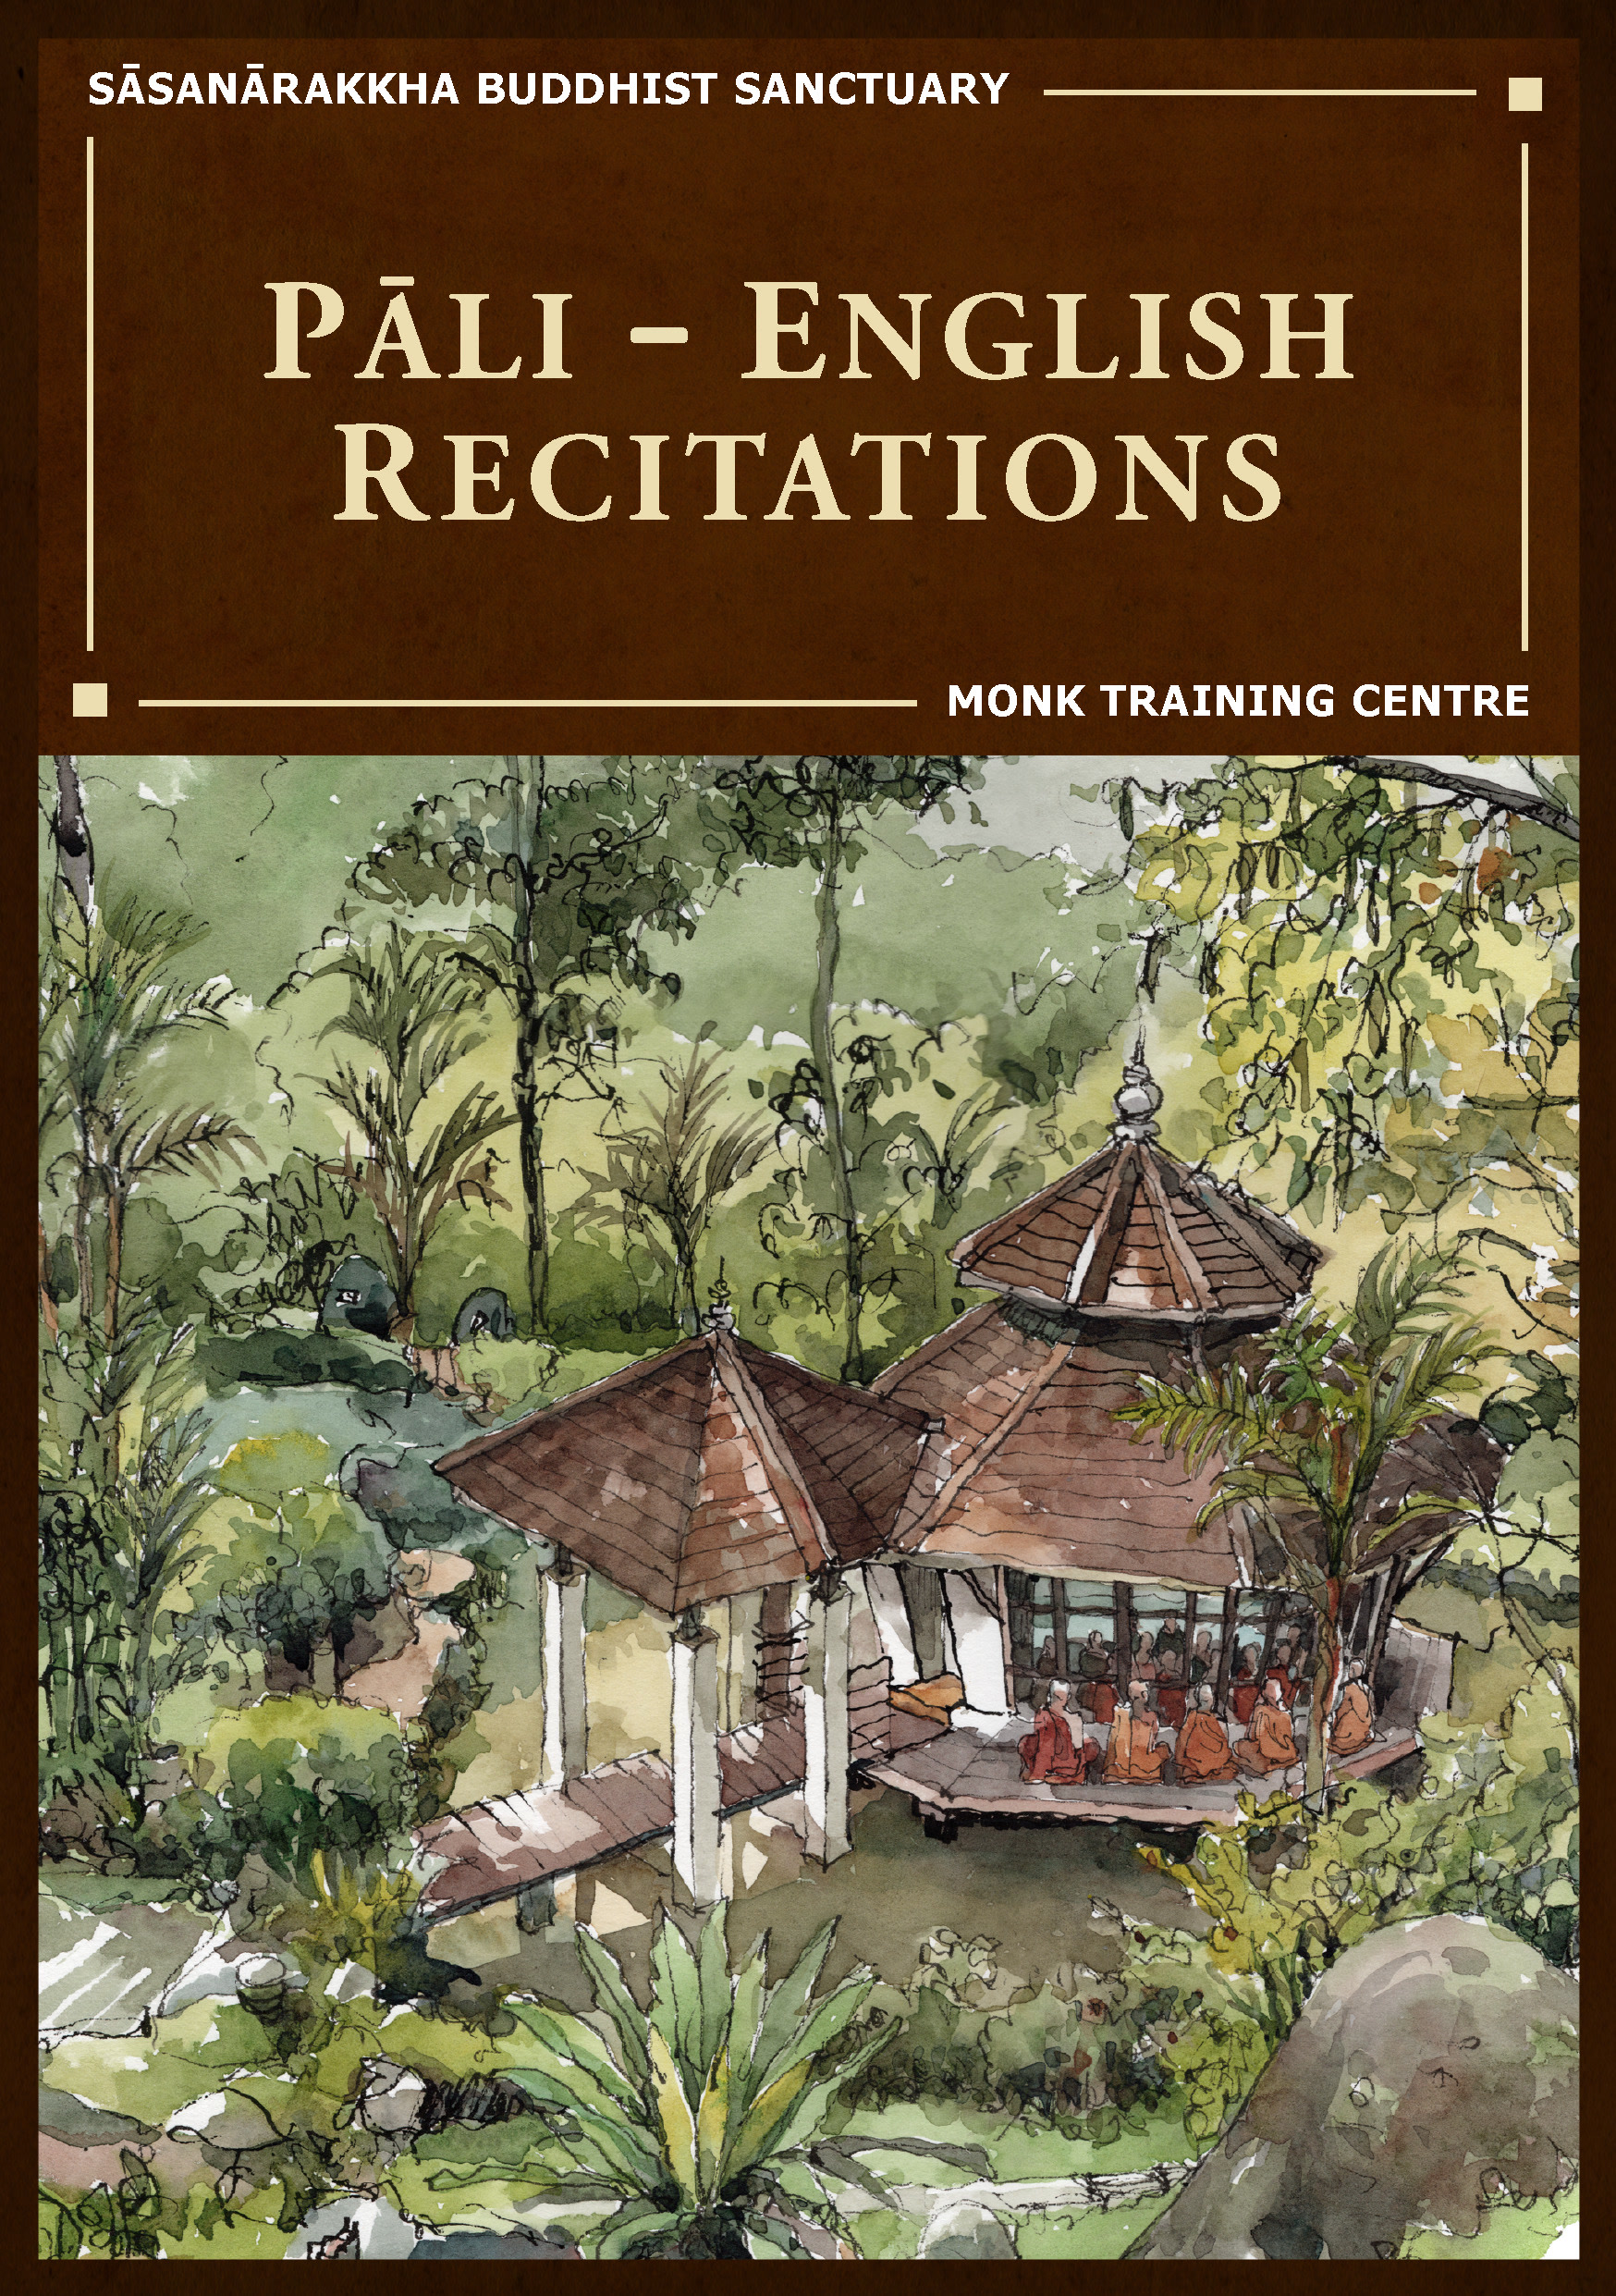
\includegraphics[height=\paperheight]{./assets/images/A5/front_cover_compressed_A5.jpg}}
\fi

\ifninebythirteenversion
  \photoFullBleed{./assets/images/9x13/front_cover_9x13.png}
  \photoFullBleed{robe_divider_left_9x13.png}
  \photoFullBleed{robe_divider_right_9x13.png}
\fi

\ifbfiveversion
  \photoFullBleed{./assets/images/B5/front_cover_B5.png}
  \photoFullBleed{robe_divider_left_B5.png}
  \photoFullBleed{robe_divider_right_B5.png}
\fi

% Title page, copyright, acknowledgments
\pagestyle{empty}
\input{./tex/titlepage.tex}
\input{./tex/copyright.tex}
\input{./tex/acknowledgments.tex}

% Table of contents, schedule, purpose and benefits, abbreviations
\cleartorecto
\pagestyle{toponerow-frontmatter}
\chapterstyle{adrasteia-toc}

\pdfbookmark[section]{\contentsname}{toc}
\tableofcontents*

\input{./tex/schedule.tex}
\input{./tex/purpose-and-benefits.tex}
\input{./tex/abbreviations.tex}

\chapterstyle{adrasteia-frontmatter}

% Main matter
\mainmatter
\pagestyle{toponerow}

\cleartorecto

% Chapters
{\raggedright
	\input{./tex/recitations/homage.tex}
	\input{./tex/recitations/verses.tex}
	\input{./tex/recitations/teachings.tex}
	\input{./tex/recitations/reflections.tex}
	\input{./tex/recitations/cardinal-discourses.tex}
	\input{./tex/recitations/thanksgiving-recitations.tex}
	\input{./tex/recitations/protective-recitations.tex}
	\input{./tex/recitations/funeral-recitations.tex}
	\input{./tex/recitations/sharing-of-merits.tex}
}

% Appendix
\appendix
\input{./tex/appendix.tex}
\input{./tex/refuge-trainings.tex}
\input{./tex/phonetics-pronunciation.tex}
\input{./tex/guidelines.tex}

% Back matter
\backmatter
\printpagenotes % Print endnotes
\input{./tex/copyright-details.tex}

\ifbfiveversion
  \includepdf[pages=-,pagecommand={\thispagestyle{empty}}]{assets/images/graphics/donor-list.pdf}
  \photoFullBleed{robe_divider_left_B5.png}
  \photoFullBleed{robe_divider_right_B5.png}
\fi

\ifninebythirteenversion
  \photoFullBleed{robe_divider_left_9x13.png}
  \photoFullBleed{robe_divider_right_9x13.png}
\fi

\emptyUntilEven % Add blank page if necessary

\ifdigitalversion
  \clearpage
  \digitalCover{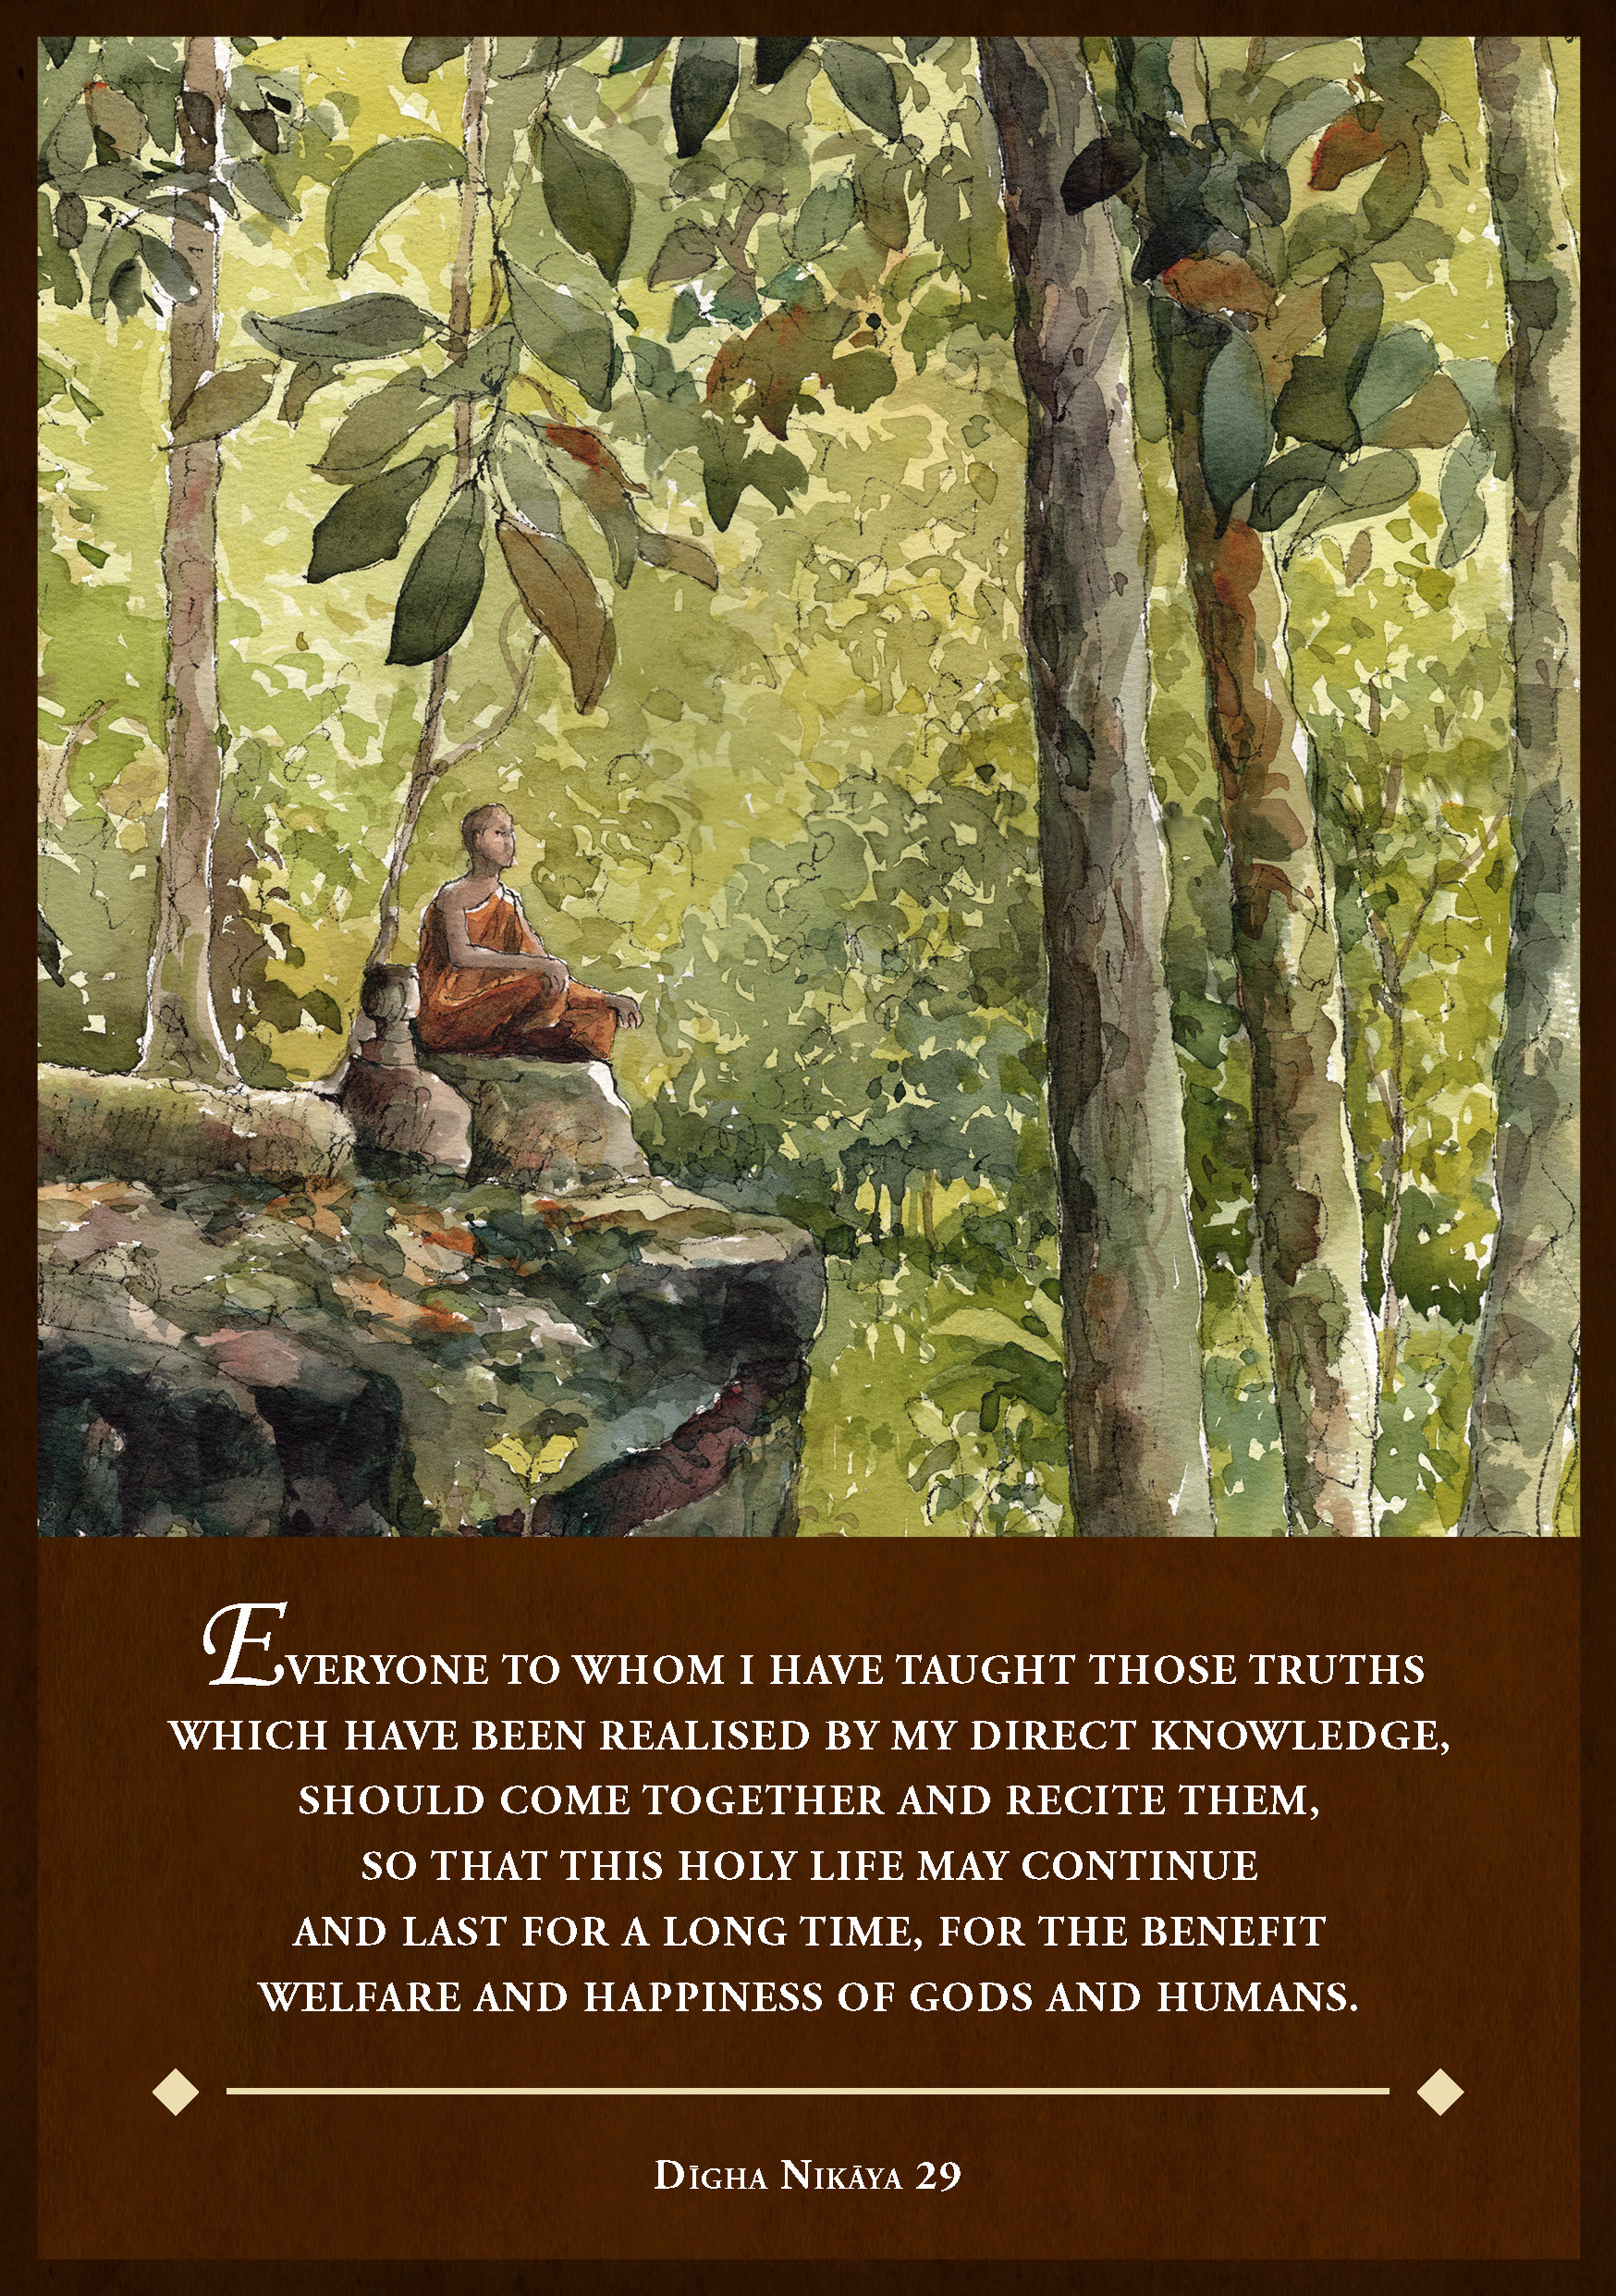
\includegraphics[height=\paperheight]{./assets/images/A5/back_cover_compressed_A5.jpg}}
\fi

\ifninebythirteenversion
  \photoFullBleed{./assets/images/9x13/back_cover_9x13.png}
\fi

\ifbfiveversion
  \photoFullBleed{./assets/images/B5/back_cover_B5.png}
\fi

\end{document}
'
% Possible VALUE:
%   - afiveVersion —  A5 formatted
%   - ninebythirteenVersion —  9x13cm custom formatted
%   - bfiveVersion —  B5 formatted
% \listfiles
\ifdefined\papersizeoption
\else
  \newcommand{\papersizeoption}{bfiveVersion}
\fi
\typeout{Set \protect\papersizeoption{} to \papersizeoption}

% Add hyperlinks and images, to be used with afiveVersion \papersizeoption
% Build command:
% '\newcommand{\papersizeoption}{afiveVersion}\newcommand{\isdigitalversion}{}% Set paper variant
% Build command '\newcommand{\papersizeoption}{VALUE}\input{main.tex}'
% Possible VALUE:
%   - afiveVersion —  A5 formatted
%   - ninebythirteenVersion —  9x13cm custom formatted
%   - bfiveVersion —  B5 formatted
% \listfiles
\ifdefined\papersizeoption
\else
  \newcommand{\papersizeoption}{bfiveVersion}
\fi
\typeout{Set \protect\papersizeoption{} to \papersizeoption}

% Add hyperlinks and images, to be used with afiveVersion \papersizeoption
% Build command:
% '\newcommand{\papersizeoption}{afiveVersion}\newcommand{\isdigitalversion}{}\input{main.tex}'
\ifdefined\isdigitalversion
  \newcommand{\digitaloption}{digitalVersion}
\else
  \newcommand{\digitaloption}{}
\fi
\typeout{Set \protect\digitaloption{} to \digitaloption}

% todo ask bergen to make showtims a togglable condition for b5 and 9x13 only

\documentclass[
  final,
  babelLanguage=british,
  showtrims,
  \papersizeoption,
  \digitaloption,
]{anecdote}

% Define graphics path for images
\graphicspath{
  {./assets/images/A5}
  {./assets/images/9x13}
  {./assets/images/B5}
  {./assets/images/graphics}
}

% Loads formatting for selected ddocument class
\ifninebythirteenversion \usepackage{9x13} \fi
\ifafiveversion \usepackage{A5} \fi
\ifbfiveversion \usepackage{B5} \fi

% Set metadata for the document
\title{SBS Pāli-English Recitations}
\subtitle{Monk Training Centre}
\author{SBS Monk Training Centre}
\publisher{Sāsanārakkha Buddhist Sanctuary}
\date{2021-10-30}
\editionInfo{\textit{First Edition}, 2025} % And last edition. Don't call Pāladhammika.
\newcommand{\MyISBN}{} % default empty

\ifbfiveversion
  \renewcommand{\MyISBN}{978-629-97831-1-4}
\fi
\ifninebythirteenversion
  \renewcommand{\MyISBN}{978-629-97831-2-1}
\fi

\ISBN{\MyISBN}

% Set metadata for PDF properties
\hypersetup{
  pdftitle={\thetitle},
  pdfauthor={\theauthor},
  pdfcopyright={Copyright (C) 2025, \thePublisher},
  pdfsubject={},
  pdfkeywords={},
  pdflicenseurl={https://creativecommons.org/licenses/by-nc-nd/4.0/},
  pdfcontacturl={},
  pdflang={en},
}

% Load further packages
\RequirePackage[yyyymmdd,hhmmss]{datetime} % Adds the time to version creation

\makepagenote
\continuousnotenums % Ensure continuous endnote numbering

% Define hyphenation exceptions and corrections
\hyphenation{London re-lin-quishes de-ter-mines}

\ifdigitalversion
  \openany
\fi

% Begin document
\begin{document}

% Front matter
\frontmatter

% Digital version cover
\ifdigitalversion
	\digitalCover{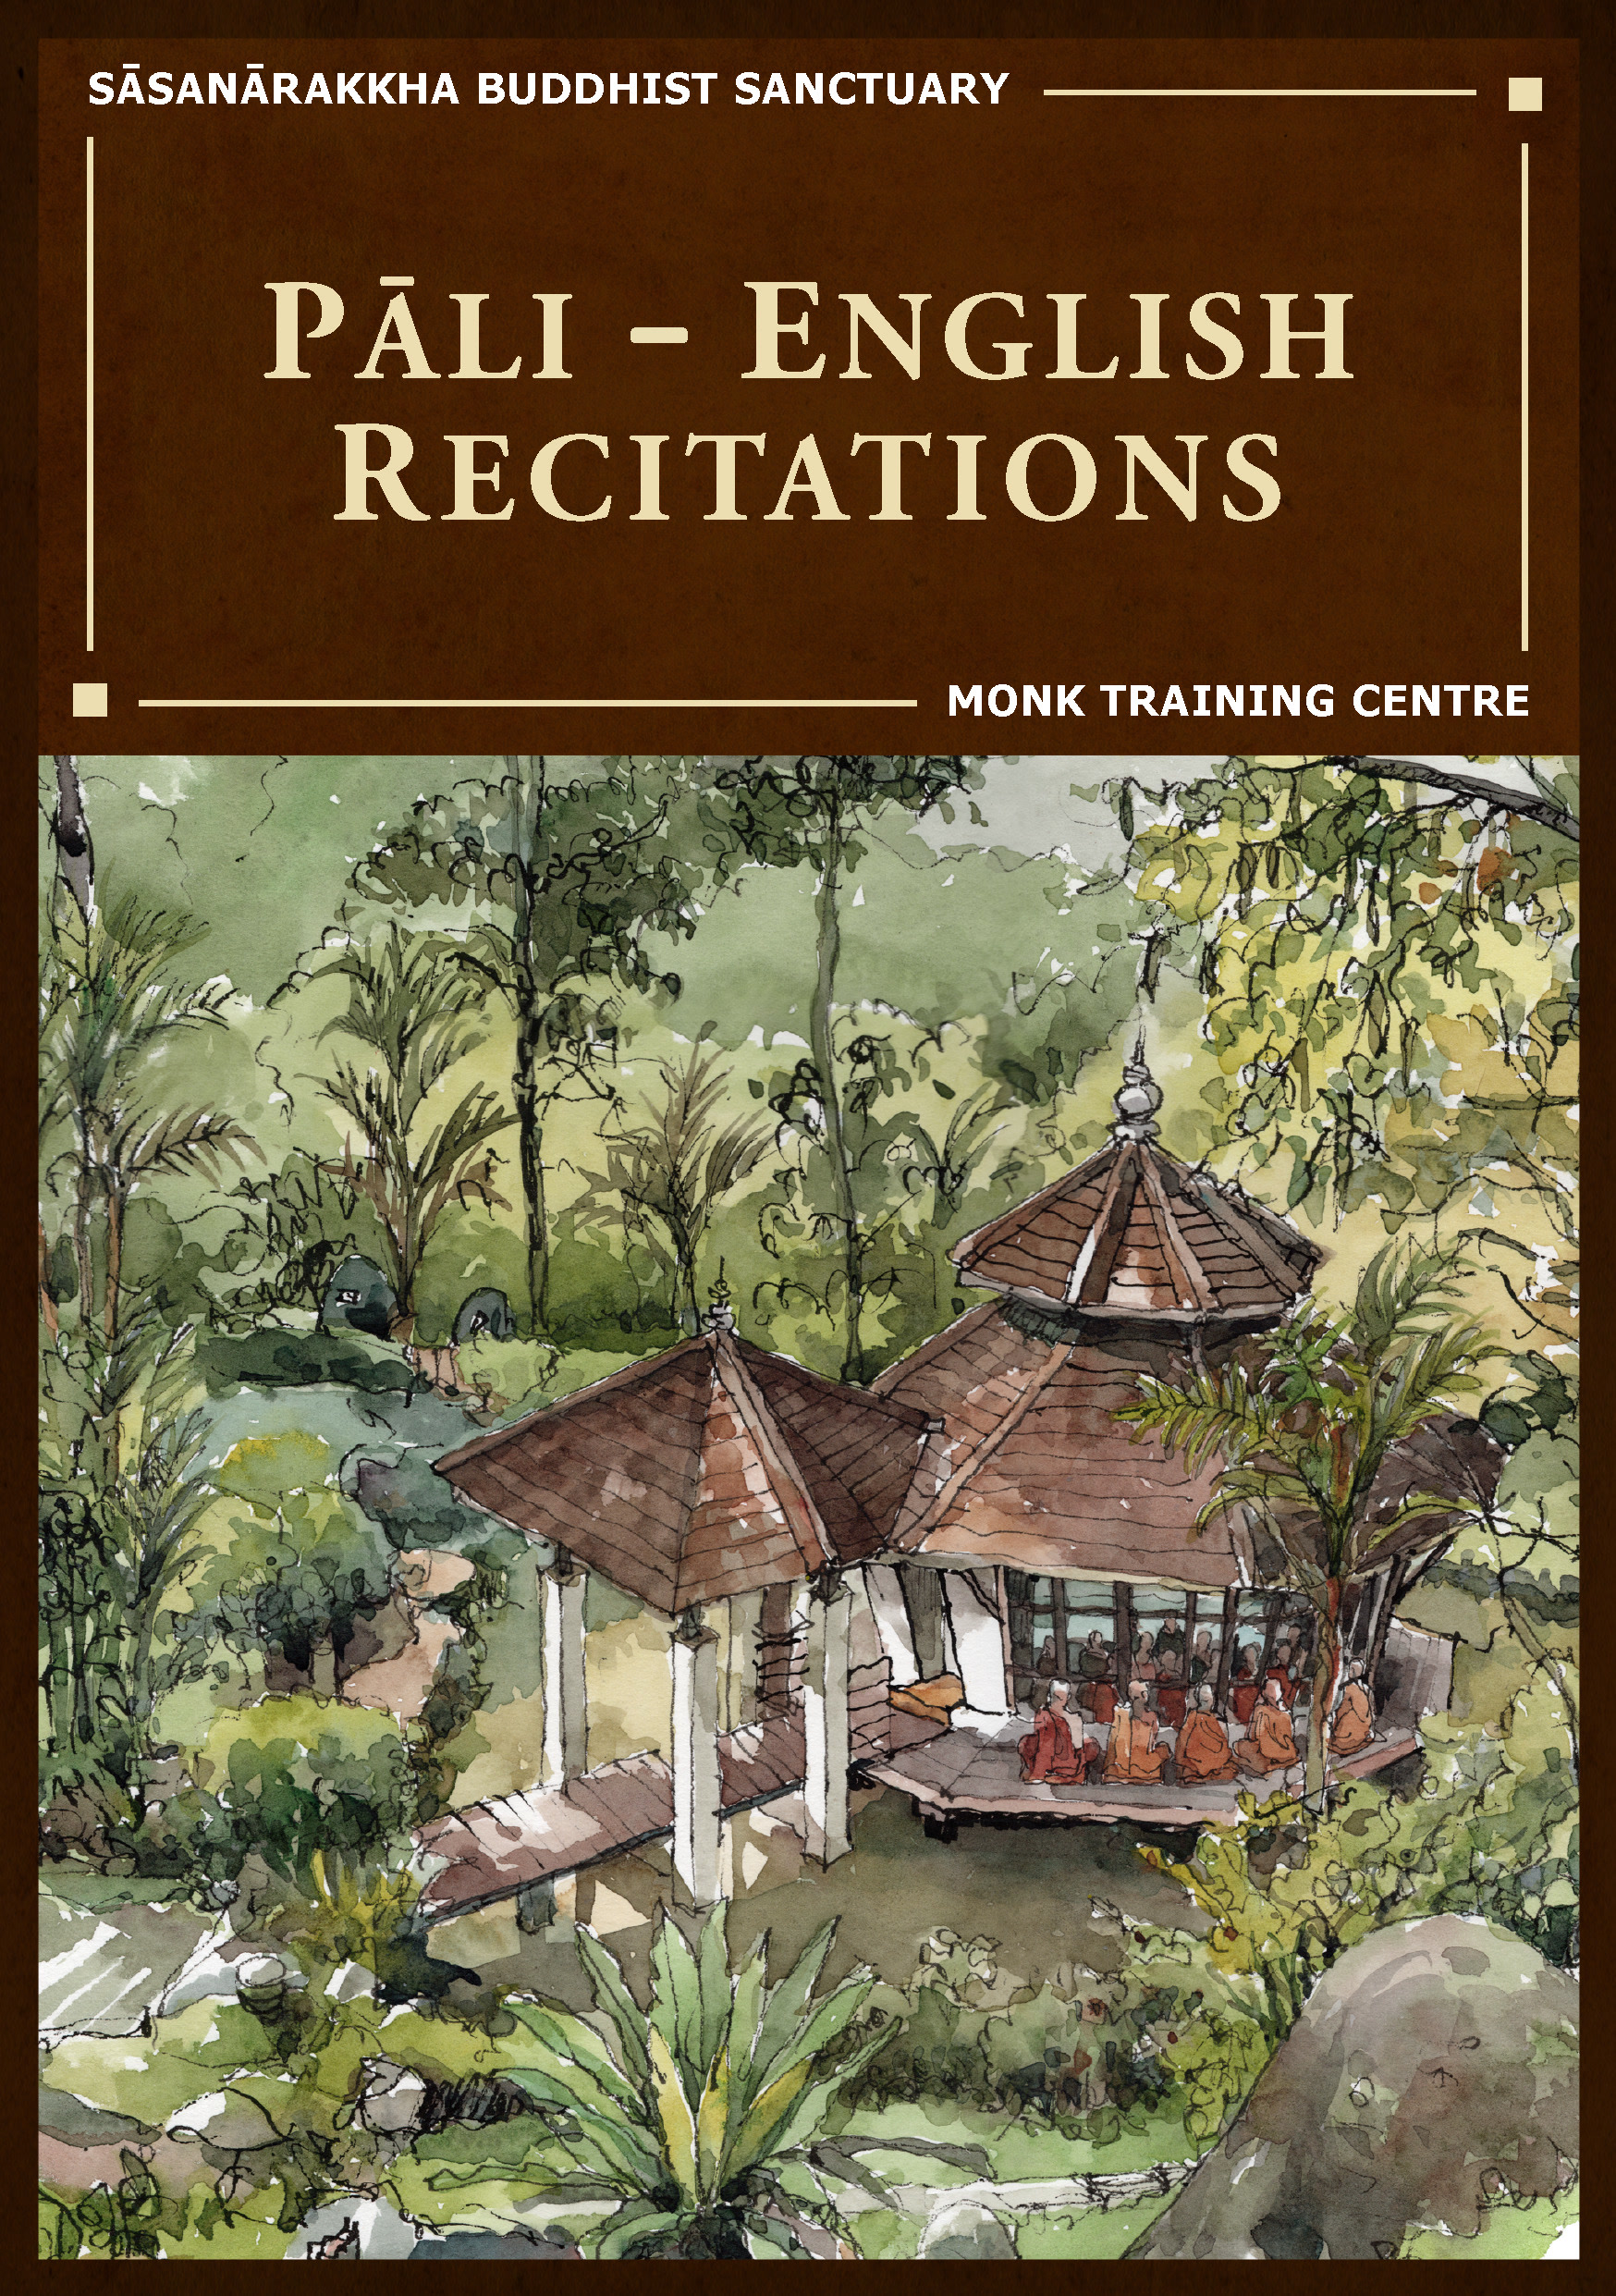
\includegraphics[height=\paperheight]{./assets/images/A5/front_cover_compressed_A5.jpg}}
\fi

\ifninebythirteenversion
  \photoFullBleed{./assets/images/9x13/front_cover_9x13.png}
  \photoFullBleed{robe_divider_left_9x13.png}
  \photoFullBleed{robe_divider_right_9x13.png}
\fi

\ifbfiveversion
  \photoFullBleed{./assets/images/B5/front_cover_B5.png}
  \photoFullBleed{robe_divider_left_B5.png}
  \photoFullBleed{robe_divider_right_B5.png}
\fi

% Title page, copyright, acknowledgments
\pagestyle{empty}
\input{./tex/titlepage.tex}
\input{./tex/copyright.tex}
\input{./tex/acknowledgments.tex}

% Table of contents, schedule, purpose and benefits, abbreviations
\cleartorecto
\pagestyle{toponerow-frontmatter}
\chapterstyle{adrasteia-toc}

\pdfbookmark[section]{\contentsname}{toc}
\tableofcontents*

\input{./tex/schedule.tex}
\input{./tex/purpose-and-benefits.tex}
\input{./tex/abbreviations.tex}

\chapterstyle{adrasteia-frontmatter}

% Main matter
\mainmatter
\pagestyle{toponerow}

\cleartorecto

% Chapters
{\raggedright
	\input{./tex/recitations/homage.tex}
	\input{./tex/recitations/verses.tex}
	\input{./tex/recitations/teachings.tex}
	\input{./tex/recitations/reflections.tex}
	\input{./tex/recitations/cardinal-discourses.tex}
	\input{./tex/recitations/thanksgiving-recitations.tex}
	\input{./tex/recitations/protective-recitations.tex}
	\input{./tex/recitations/funeral-recitations.tex}
	\input{./tex/recitations/sharing-of-merits.tex}
}

% Appendix
\appendix
\input{./tex/appendix.tex}
\input{./tex/refuge-trainings.tex}
\input{./tex/phonetics-pronunciation.tex}
\input{./tex/guidelines.tex}

% Back matter
\backmatter
\printpagenotes % Print endnotes
\input{./tex/copyright-details.tex}

\ifbfiveversion
  \includepdf[pages=-,pagecommand={\thispagestyle{empty}}]{assets/images/graphics/donor-list.pdf}
  \photoFullBleed{robe_divider_left_B5.png}
  \photoFullBleed{robe_divider_right_B5.png}
\fi

\ifninebythirteenversion
  \photoFullBleed{robe_divider_left_9x13.png}
  \photoFullBleed{robe_divider_right_9x13.png}
\fi

\emptyUntilEven % Add blank page if necessary

\ifdigitalversion
  \clearpage
  \digitalCover{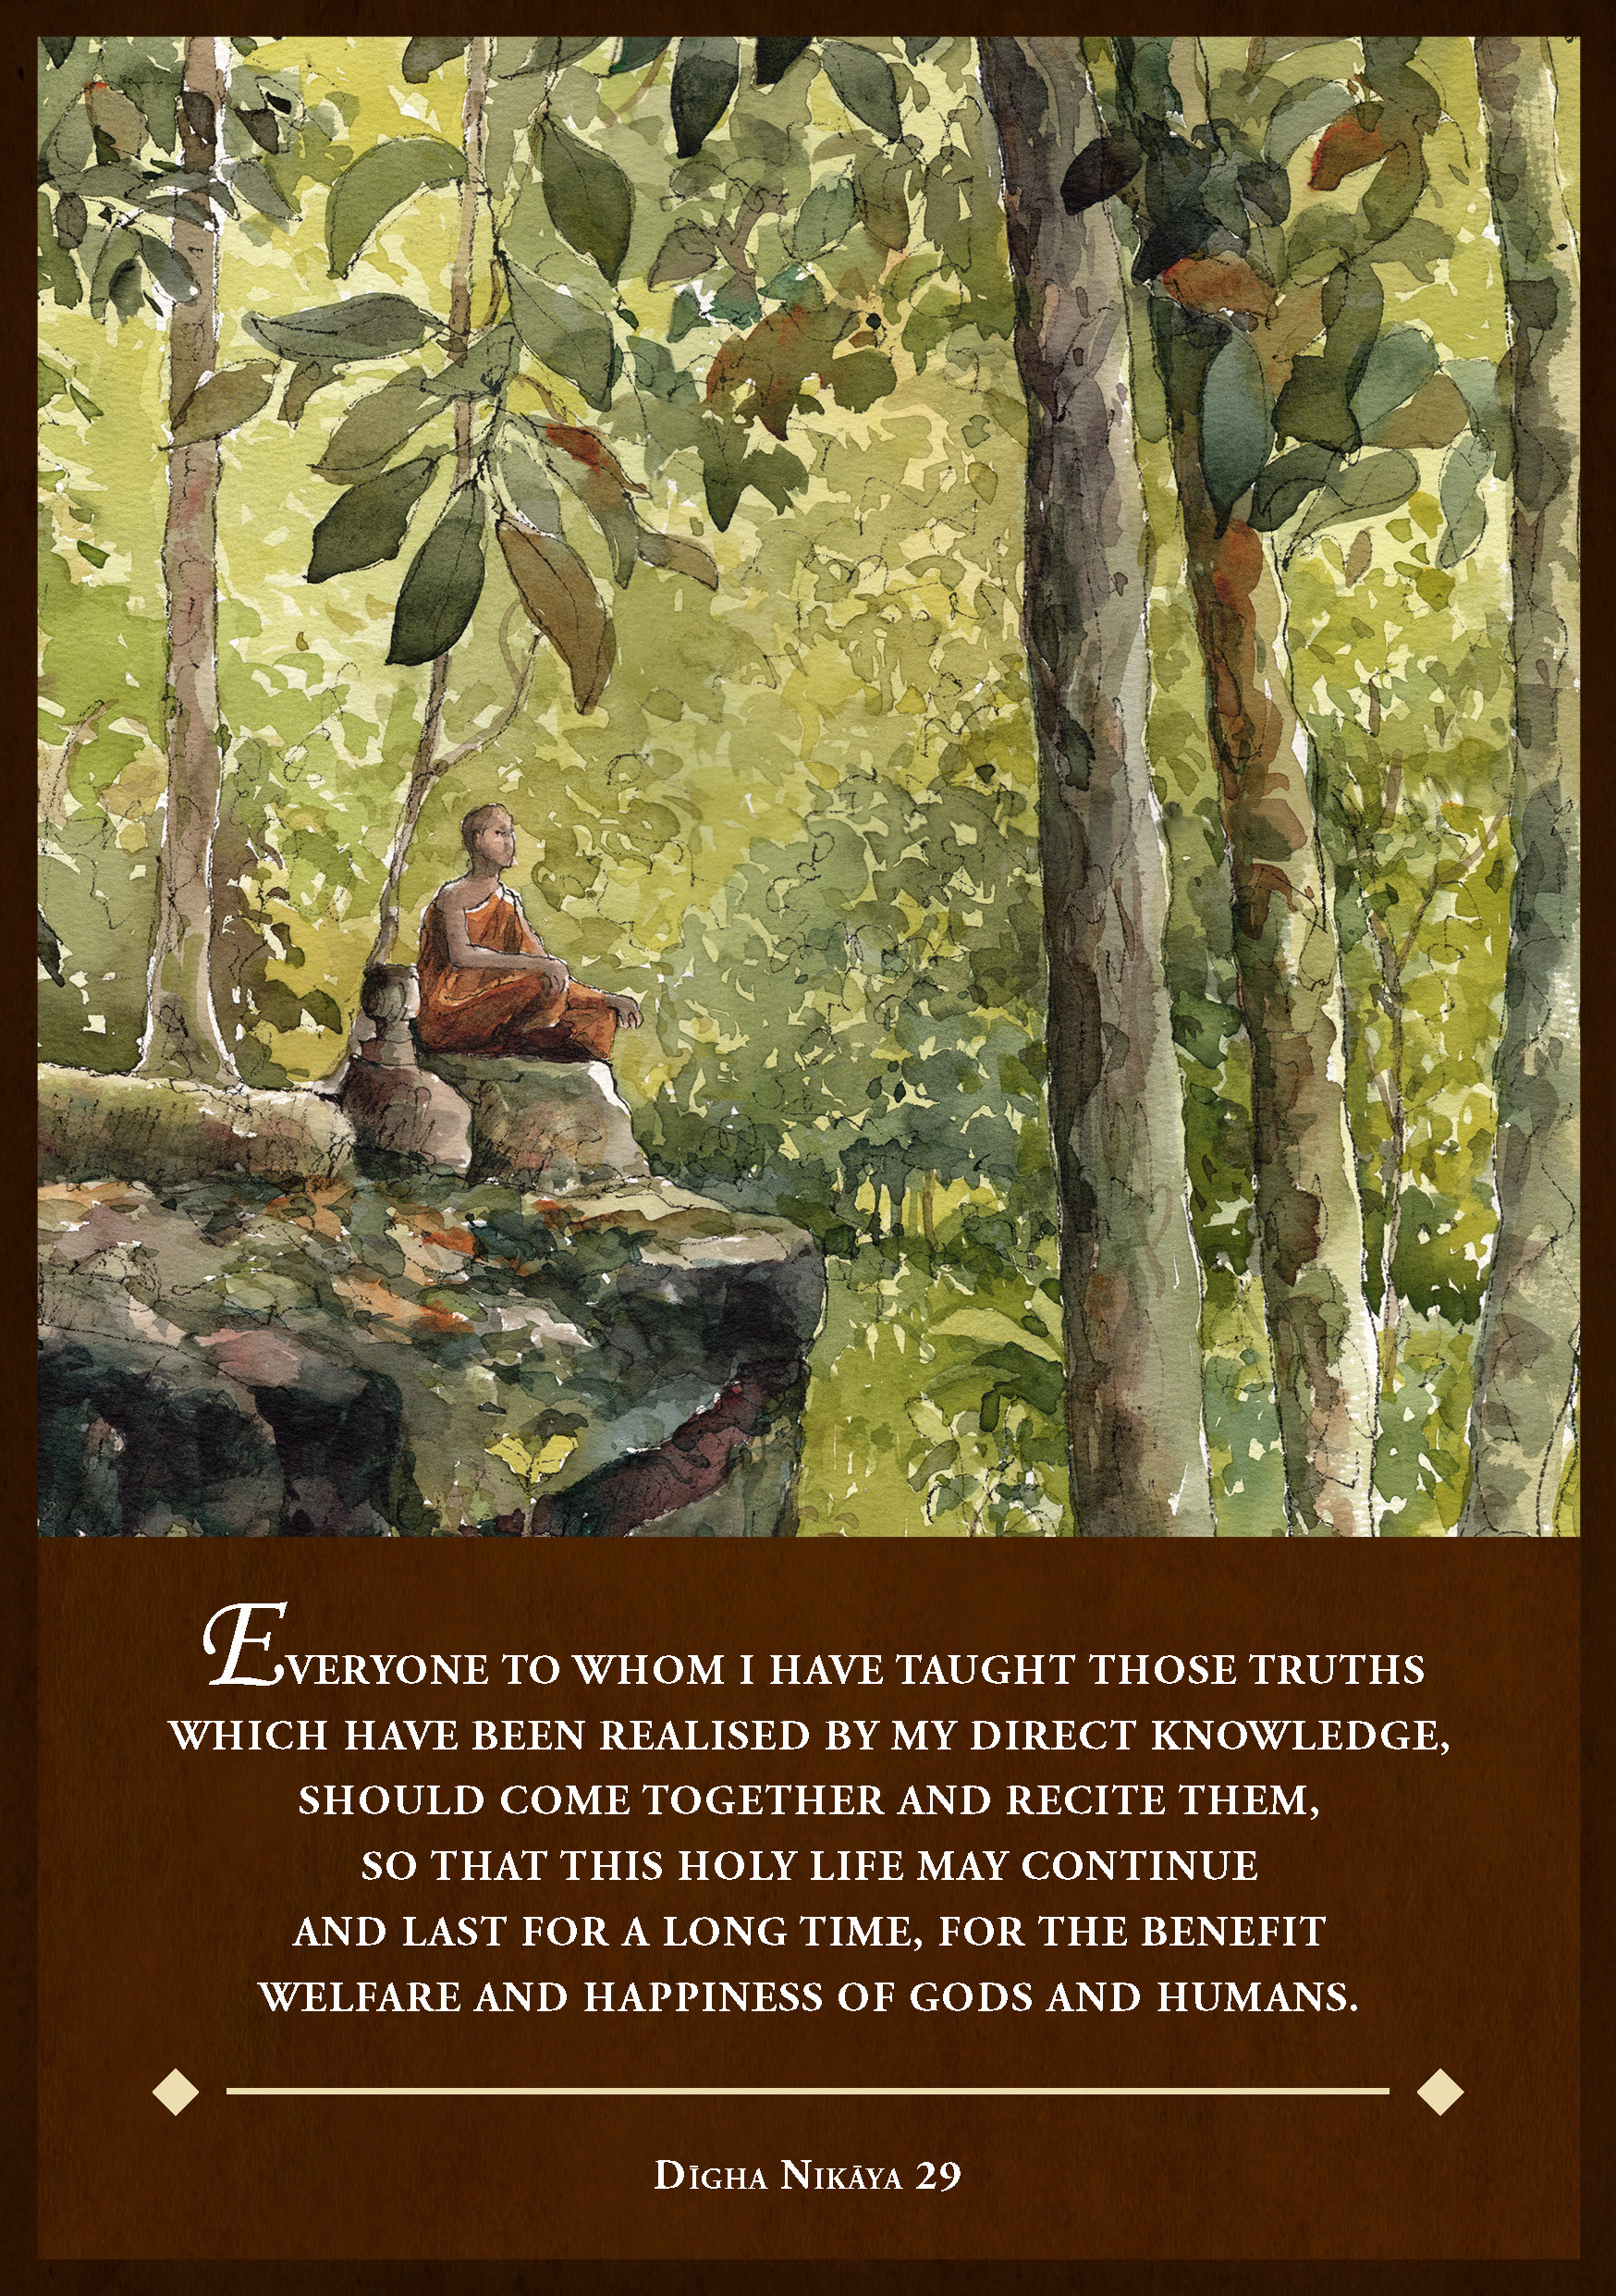
\includegraphics[height=\paperheight]{./assets/images/A5/back_cover_compressed_A5.jpg}}
\fi

\ifninebythirteenversion
  \photoFullBleed{./assets/images/9x13/back_cover_9x13.png}
\fi

\ifbfiveversion
  \photoFullBleed{./assets/images/B5/back_cover_B5.png}
\fi

\end{document}
'
\ifdefined\isdigitalversion
  \newcommand{\digitaloption}{digitalVersion}
\else
  \newcommand{\digitaloption}{}
\fi
\typeout{Set \protect\digitaloption{} to \digitaloption}

% todo ask bergen to make showtims a togglable condition for b5 and 9x13 only

\documentclass[
  final,
  babelLanguage=british,
  showtrims,
  \papersizeoption,
  \digitaloption,
]{anecdote}

% Define graphics path for images
\graphicspath{
  {./assets/images/A5}
  {./assets/images/9x13}
  {./assets/images/B5}
  {./assets/images/graphics}
}

% Loads formatting for selected ddocument class
\ifninebythirteenversion \usepackage{9x13} \fi
\ifafiveversion \usepackage{A5} \fi
\ifbfiveversion \usepackage{B5} \fi

% Set metadata for the document
\title{SBS Pāli-English Recitations}
\subtitle{Monk Training Centre}
\author{SBS Monk Training Centre}
\publisher{Sāsanārakkha Buddhist Sanctuary}
\date{2021-10-30}
\editionInfo{\textit{First Edition}, 2025} % And last edition. Don't call Pāladhammika.
\newcommand{\MyISBN}{} % default empty

\ifbfiveversion
  \renewcommand{\MyISBN}{978-629-97831-1-4}
\fi
\ifninebythirteenversion
  \renewcommand{\MyISBN}{978-629-97831-2-1}
\fi

\ISBN{\MyISBN}

% Set metadata for PDF properties
\hypersetup{
  pdftitle={\thetitle},
  pdfauthor={\theauthor},
  pdfcopyright={Copyright (C) 2025, \thePublisher},
  pdfsubject={},
  pdfkeywords={},
  pdflicenseurl={https://creativecommons.org/licenses/by-nc-nd/4.0/},
  pdfcontacturl={},
  pdflang={en},
}

% Load further packages
\RequirePackage[yyyymmdd,hhmmss]{datetime} % Adds the time to version creation

\makepagenote
\continuousnotenums % Ensure continuous endnote numbering

% Define hyphenation exceptions and corrections
\hyphenation{London re-lin-quishes de-ter-mines}

\ifdigitalversion
  \openany
\fi

% Begin document
\begin{document}

% Front matter
\frontmatter

% Digital version cover
\ifdigitalversion
	\digitalCover{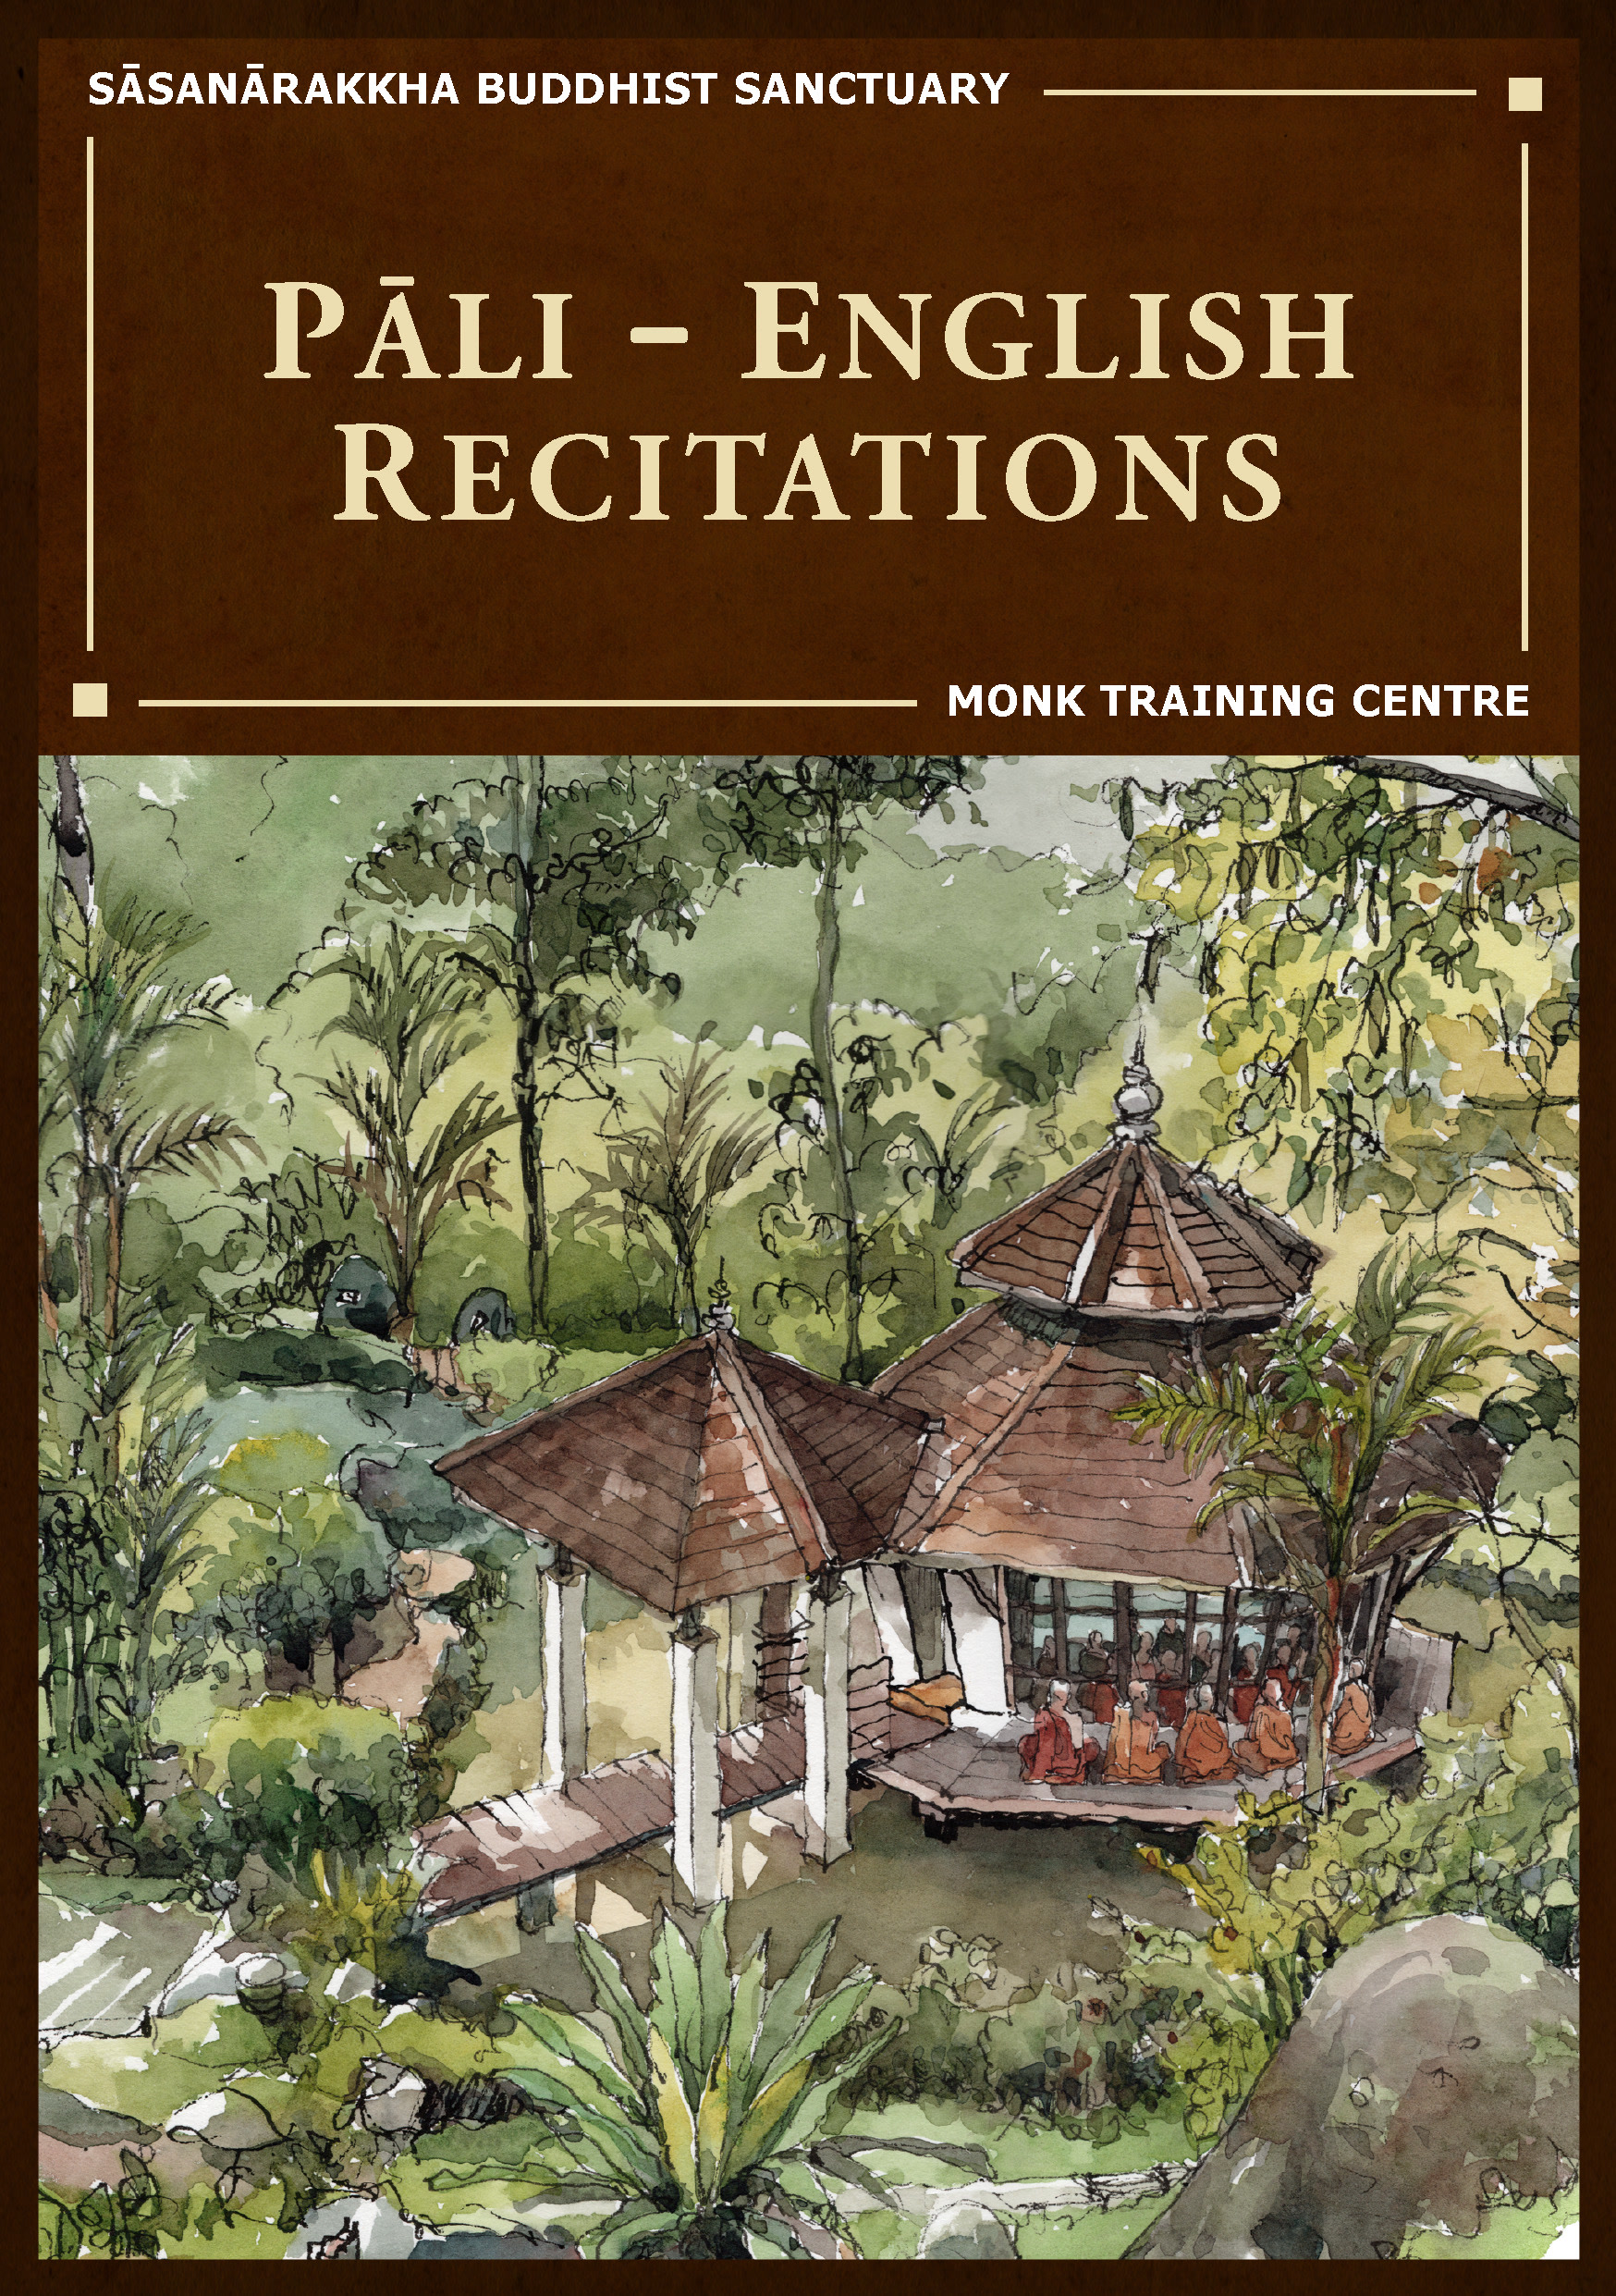
\includegraphics[height=\paperheight]{./assets/images/A5/front_cover_compressed_A5.jpg}}
\fi

\ifninebythirteenversion
  \photoFullBleed{./assets/images/9x13/front_cover_9x13.png}
  \photoFullBleed{robe_divider_left_9x13.png}
  \photoFullBleed{robe_divider_right_9x13.png}
\fi

\ifbfiveversion
  \photoFullBleed{./assets/images/B5/front_cover_B5.png}
  \photoFullBleed{robe_divider_left_B5.png}
  \photoFullBleed{robe_divider_right_B5.png}
\fi

% Title page, copyright, acknowledgments
\pagestyle{empty}

\cleartorecto
\thispagestyle{empty}

\vspace*{3em}

{\centering

  \settowidth{\titleLength}{%
    {\Large\chapterTitleFont\textsc{\MakeUppercase{{Pāli-English Recitations}}}}%
  }

  % 'SBS' on title page
  \ifafive {\Huge\fontsize{64}{16}\sbsFont SBS}\\[1.0\baselineskip] \fi
  \ifninebythirteen {\Huge\fontsize{42.5}{11}\sbsFont SBS}\\[1.0\baselineskip] \fi
  \ifbfive {\Huge\fontsize{80}{16}\sbsFont SBS}\\[1.0\baselineskip] \fi

  % 'Monk Training Centre'
  \ifafive \setlength{\xheight}{\heightof{X}}
    {\Huge\chapterTitleFont\textsc{{\thesubtitle\linebreak}}}\\[0.2\baselineskip] \fi
  \ifninebythirteen {\fontsize{16}{14}\chapterTitleFont\textsc{{\thesubtitle\linebreak}}}\\[0.2\baselineskip] \fi
  \ifbfive \setlength{\xheight}{\heightof{X}}
    {\fontsize{30}{14}\chapterTitleFont\textsc{{\thesubtitle\linebreak}}}\\[0.2\baselineskip] \fi

  % Ornament
  \ifafive \raisebox{0.5\xheight}{\pgfornament[color=sbs-brown,width=7cm,scale=1,ydelta=0pt,symmetry=c]{84}}\\[1.4\baselineskip] \fi
  \ifninebythirteen \raisebox{0.5\xheight}{\pgfornament[color=sbs-brown,width=4.5cm,scale=1,ydelta=0pt,symmetry=c]{84}}\\[1.4\baselineskip] \fi
  \ifbfive \raisebox{0.5\xheight}{\pgfornament[color=sbs-brown,width=8.5cm,scale=1,ydelta=0pt,symmetry=c]{84}}\\[1.4\baselineskip] \fi


  % 'Pali-English Recitations'
  \ifafive {\Large\scshape Pāli-English Recitations}\\[2.5\baselineskip] \fi
  \ifninebythirteen {\fontsize{10}{12}\scshape Pāli-English Recitations}\\[2.5\baselineskip] \fi
  \ifbfive {\fontsize{18.5}{12}\scshape Pāli-English Recitations}\\[2.5\baselineskip] \fi

  % Dhamma quote
  {\quote ``In whatever way a bhikkhu recites the Dhamma in detail as he has heard it and learned it, in just that way, in relation to that Dhamma, he experiences inspiration in the meaning and inspiration in the Dhamma. As he does so, joy arises in him. When he is joyful, rapture arises. For one with a rapturous mind, the body becomes tranquil. One tranquil in body feels pleasure. For one feeling pleasure, the mind becomes concentrated.''\\}
  \ifafive \smallskip AN 5.26\\[1.4\baselineskip]\fi
  \ifninebythirteen \smallskip \fontsize{8}{14}\selectfont AN 5.26\\[1.4\baselineskip]\fi
  %% \ifbfive \smallskip \fontsize{8.5}{14}\selectfont AN 5.26\\[1.4\baselineskip]\fi
  \ifbfive \smallskip AN 5.26\\[1.4\baselineskip]\fi
}



\cleartoverso
\thispagestyle{empty}

{%

  \ifafive \fontsize{10}{16}\selectfont \fi
  \ifninebythirteen \fontsize{7.5}{11}\selectfont \fi
  \ifbfive \fontsize{12}{20}\selectfont \fi
  \centering
  \setlength{\parindent}{0pt}%

  \ifafive \vspace{0.5cm} \fi
  \ifninebythirteen \vspace{0.4cm} \fi
  \ifbfive \vspace{0.5cm} \fi

  \copyright\ \thePublisher, 2025\\
  c/o 160, Lorong 3, Jalan Merdeka, 34000 Taiping, Perak, Malaysia\\
  \ifdigital
    \else
  ISBN \theISBN
  \fi

  \ifafive \vspace{0.5cm} \fi
  \ifninebythirteen \vspace{0.3cm} \fi
  \ifbfive \vspace{0.5cm} \fi

  This book is for free distribution only;\\
  it may not be sold.

  \ifafive \vspace{0.5cm} \fi
  \ifninebythirteen \vspace{0.3cm} \fi
  \ifbfive \vspace{0.5cm} \fi

  Download this book as a PDF, EPUB, MOBI, AZW3\\
  at the following address:\\
  \href{https://sasanarakkha.org/recitations}{https://sasanarakkha.org/recitations}

Accompanying audio recordings can be found at:
\href{https://www.youtube.com/SasanarakkhaBuddhistSanctuary}{https://www.youtube.com/SasanarakkhaBuddhistSanctuary}

  \ifafive \vspace{0.5cm} \fi
  \ifninebythirteen \vspace{0.3cm} \fi
  \ifbfive \vspace{0.5cm} \fi

  Project Manager: Ā. Ariyadhammika\\
  Editor: Ā. Pāladhammika\\
  Typesetting: Aj. Gambhiro, Ā. Pāladhammika\\
  Translators: Ā. Aggacitta, Ā. Bodhi, Aj. Kevalī, Ā. Sujāto, M. Walshe\\
  Endnotes: Ā. Ariyadhammika\\
  Watercolor Paintings: Lim Jee Yuan

  \ifafive \vspace{0.5cm} \fi
  \ifninebythirteen \vspace{0.3cm} \fi
  \ifbfive \vspace{0.5cm} \fi

  This work is licensed under a Creative Commons\\
  Attribution-NonCommercial-NoDerivatives 4.0 International~License.

  % Produced with the \LaTeX\ typesetting system,\\
  % set in Libertinus Serif.

  \ifafive  \vspace{0.5cm} \fi
  \ifninebythirteen \vspace{0.3cm} \fi
  \ifbfive \vspace{0.5cm} \fi

  \ifdigital
    This version was created on:\\
    \today \space at \currenttime\\
  \fi

  \ifafive \vspace{0.5cm} \fi
  \ifninebythirteen \vspace{0.15cm} \fi
  \ifbfive \vspace{0.5cm} \fi

  \theEditionInfo

}

\ifdigital

\else

\clearpage

\fi



\cleartorecto
\thispagestyle{empty}

{

  \setlength{\parskip}{10pt}

  \ifafive {\centering\fontsize{16}{25}\selectfont \textsc{We Wish To Gratefully Acknowledge} \par} \fi
  \ifninebythirteen {\centering\fontsize{10}{18}\selectfont \textsc{We Wish To Gratefully Acknowledge} \par} \fi
  \ifbfive {\centering\fontsize{18.5}{25}\selectfont \textsc{We Wish To Gratefully Acknowledge} \par} \fi


  The Saṅghas of Wat Pah Nanachat (WPN), Amaravati, and Abhayagiri for allowing the use of material from their respective chanting books, the late Ven. Dr. Saddhātissa and Mr. Maurice Walshe for their English translations, as well as Ven. Bhikkhu Bodhi for granting permission to use and slightly adapt his translations. Various Saṅgha members of SBS Monk Training Centre, who contributed in the compilation of an interesting selection of chants, as well as for providing countless suggestions to help improve the English translations.

  \linkdest{endnote1-body}
  Additional information on translations, as well as deviations\makeatletter\hyperlink{endnote1-appendix}\Hy@raisedlink{{\pagenote{%
        \hypertarget{endnote1-appendix}{\hyperlink{endnote1-body}{Due to the balanced and inspiring selection of chants, as well as for the sake of compatibility, WPN’s \textit{Buddhist Chanting} (2014) has served as the basis for this book. Over time, suggestions for the inclusion of additional chants, as well as occasional improvements of existing translations were incorporated. Such changes were meticulously marked down in the endnotes of the digital versions of this chanting book, so that someone familiar with the present book can straight away find the relevant differences, which can be useful when visiting a branch monastery of the Ajahn Chah lineage, in order to know in which places to revert to the original version.}}}}}\makeatother\thickspace
  from WPN's \textit{Buddhist Chanting} (2014), have been annotated by Ven. Ariyadhammika in the endnotes.


  \ifninebythirteen \smallskip \else \medskip \fi

  {\centering

    To Āyasmā Aggacitta, the founding father of\\
    Sāsanārakkha Buddhist Sanctuary.

    % \ifninebythirteen \smallskip \else \medskip \fi

    \begin{center}
      \ifafive 
\includegraphics[height=54mm]{sbs_logo_tuck_loon_brown.jpg} \fi
      \ifninebythirteen \clearpage \vspace*{\fill}
 
\includegraphics[height=80mm]{sbs_logo_tuck_loon_brown.jpg} \vspace*{\fill} \fi
      \ifbfive \vspace{1cm} 
\includegraphics[height=70mm]{sbs_logo_tuck_loon_brown.jpg}\fi
    \end{center}
  }
}



% Table of contents, schedule, purpose and benefits, abbreviations
\cleartorecto
\pagestyle{toponerow-frontmatter}
\chapterstyle{adrasteia-toc}

\pdfbookmark[section]{\contentsname}{toc}
\tableofcontents*


\chapter{Recitation Schedule}
\label{schedule}

{\centering

  {\pdfbookmark[2]{Set 1}{set1}\libertinusFont\selectfont\textbf{\textsc{\ifafive\fontsize{18}{12}\fi\ifninebythirteen\fontsize{13}{8.5}\fi\ifbfive\fontsize{22}{18}\fi\selectfont\textls*{Set 1}}}}\\
  \textsc{\ifafive\fontsize{14.4}{28}\fi\ifninebythirteen\fontsize{8.7}{17}\fi\ifbfive\fontsize{16}{33.5}\fi\selectfont
    \hyperref[buddhas-first-exclamation]{The Buddha's First Exclamation} \ifdigital\else\pageref{buddhas-first-exclamation}\fi\\
    \hyperref[wheel-of-dhamma-abridged]{Turning the Wheel of Dhamma} \ifdigital\else\pageref{wheel-of-dhamma-abridged}\fi\\
    \hyperref[true-false-refuges]{Going to True and False Refuges} \ifdigital\else\pageref{true-false-refuges}\fi\\
    \hyperref[four-great-references]{The Four Great References} \ifdigital\else\pageref{four-great-references}\fi\\
    \hyperref[patimokkha-exhortation]{The Pāṭimokkha Exhortation} \ifdigital\else\pageref{patimokkha-exhortation}\fi\\
    \hyperref[buddhas-final-instruction]{The Buddha's Final Instruction} \ifdigital\else\pageref{buddhas-final-instruction}\fi\\
    \hyperref[uddissanadhitthana]{Sharing and Aspirations (Pāli)} \ifdigital\else\pageref{uddissanadhitthana}\fi\\
    \hyperref[closing-homage]{Closing Homage (Pāli-English)} \ifdigital\else\pageref{closing-homage}\fi\\
  }

  \ifafive\vspace{1.0cm}\fi
  \ifninebythirteen\vspace{0.8cm}\fi
  \ifbfive\vspace{1.0cm}\fi

  {\pdfbookmark[2]{Set 2}{set2}\libertinusFont\selectfont\textbf{\textsc{\ifafive\fontsize{18}{12}\fi\ifninebythirteen\fontsize{13}{8.5}\fi\ifbfive\fontsize{22}{18}\fi\selectfont\textls*{Set 2}}}}\\
  \textsc{\ifafive\fontsize{14.4}{28}\fi\ifninebythirteen\fontsize{8.7}{17}\fi\ifbfive\fontsize{16}{33.5}\fi\selectfont
    \hyperref[characteristic-of-not-self]{The Discourse on the Characteristic of Not-Self} \ifdigital\else\pageref{characteristic-of-not-self}\fi\\
    \hyperref[exposition-on-burning]{The Discourse on the Exposition on Burning} \ifdigital\else\pageref{exposition-on-burning}\fi\\
    \hyperref[gradual-training]{The Gradual Training} \ifdigital\else\pageref{gradual-training}\fi\\
    \hyperref[sharing-aspirations]{Sharing and Aspirations (English)} \ifdigital\else\pageref{sharing-aspirations}\fi\\
    \hyperref[closing-homage]{Closing Homage (English)} \ifdigital\else\pageref{closing-homage}\fi\\
  }

  \clearpage

  {\pdfbookmark[2]{Set 3}{set3}\libertinusFont\selectfont\textbf{\textsc{\ifafive\fontsize{18}{12}\fi\ifninebythirteen\fontsize{13}{8.5}\fi\ifbfive\fontsize{22}{18}\fi\selectfont\textls*{Set 3}}}}\\

\textsc{\ifafive\fontsize{14.4}{28}\fi\ifninebythirteen\fontsize{8.7}{17}\fi\ifbfive\fontsize{16}{33.5}\fi\selectfont
    \hyperref[noble-eightfold-path]{The Noble Eightfold Path} \ifdigital\else\pageref{noble-eightfold-path}\fi\\
    \hyperref[repulsiveness-of-food]{The Repulsiveness of Food} \ifdigital\else\pageref{repulsiveness-of-food}\fi\\
    \hyperref[requisites-for-awakening]{Requisites for Awakening} \ifdigital\else\pageref{requisites-for-awakening}\fi\\
    \hyperref[principles-of-non-decline]{Principles of Non-Decline} \ifdigital\else\pageref{principles-of-non-decline}\fi\\
    \hyperref[protection]{On Protection} \ifdigital\else\pageref{protection}\fi\\
    \hyperref[sharing-all-merits]{Sharing of All Merits} \ifdigital\else\pageref{sharing-all-merits}\fi\\
    \hyperref[closing-homage]{Closing Homage (Pāli-English)} \ifdigital\else\pageref{closing-homage}\fi\\
  }

  \ifafive\vspace{1.0cm}\fi
  \ifninebythirteen\vspace{0.8cm}\fi
  \ifbfive\vspace{1.0cm}\fi

  {\pdfbookmark[2]{Set 4}{set4}\libertinusFont\selectfont\textbf{\textsc{\ifafive\fontsize{18}{12}\fi\ifninebythirteen\fontsize{13}{8.5}\fi\ifbfive\fontsize{22}{18}\fi\selectfont\textls*{Set 4}}}}\\

\textsc{\ifafive\fontsize{14.4}{28}\fi\ifninebythirteen\fontsize{8.7}{17}\fi\ifbfive\fontsize{16}{33.5}\fi\selectfont
    \hyperref[dedication-of-offerings]{Homage to the Triple Gem} \ifdigital\else\pageref{dedication-of-offerings}\fi\\
    \hyperref[universal-well-being]{Universal Well-Being} \ifdigital\else\pageref{universal-well-being}\fi\\
    \hyperref[seven-factors-of-awakening]{The Seven Factors of Awakening} \ifdigital\else\pageref{seven-factors-of-awakening}\fi\\
    \hyperref[words-on-loving-kindness]{The Buddha's Words on Loving-Kindness} \ifdigital\else\pageref{words-on-loving-kindness}\fi\\
    \hyperref[sharing-merits-departed]{Sharing of Merits with \ifninebythirteen\\[-0.6em]\fi the Departed (Pāli-English)} \ifdigital\else\pageref{sharing-merits-departed}\fi\\
    \hyperref[sharing-merits-devas]{Sharing of Merits with the Devas (Pāli-English)} \ifdigital\else\pageref{sharing-merits-devas}\fi\\
    \hyperref[closing-homage]{Closing Homage (Pāli-English)} \ifdigital\else\pageref{closing-homage}\fi\\
  }

  \clearpage

  {\pdfbookmark[2]{Set 5}{set5}\libertinusFont\selectfont\textbf{\textsc{\ifafive\fontsize{18}{12}\fi\ifninebythirteen\fontsize{13}{8.5}\fi\ifbfive\fontsize{22}{18}\fi\selectfont\textls*{Set 5}}}}\\
  \textsc{\ifafive\fontsize{14.4}{28}\fi\ifninebythirteen\fontsize{8.7}{17}\fi\ifbfive\fontsize{16}{33.5}\fi\selectfont
    \hyperref[mindfulness-of-breathing]{Mindfulness of Breathing} \ifdigital\else\pageref{mindfulness-of-breathing}\fi\\
    \hyperref[discourse-on-blessings]{The Discourse on Blessings} \ifdigital\else\pageref{discourse-on-blessings}\fi\\
    \hyperref[three-characteristics]{The Three Characteristics} \ifdigital\else\pageref{three-characteristics}\fi\\
    \hyperref[four-requisites]{The Four Requisites} \ifdigital\else\pageref{four-requisites}\fi\\
    \hyperref[five-reflections]{Five Subjects for Frequent Reflection} \ifdigital\else\pageref{five-reflections}\fi\\
    \hyperref[32-parts]{The Thirty-Two Body Parts} \ifdigital\else\pageref{32-parts}\fi\\
    \hyperref[principles-of-cordiality]{Principles of Cordiality} \ifdigital\else\pageref{principles-of-cordiality}\fi\\
    \hyperref[highest-honour-aspirations]{The Highest Honour and Aspirations} \ifdigital\else\pageref{highest-honour-aspirations}\fi\\
    \hyperref[closing-homage]{Closing Homage (Pāli-English)} \ifdigital\else\pageref{closing-homage}\fi\\
  }

  \ifafive\vspace{1.0cm}\fi
  \ifninebythirteen\vspace{0.8cm}\fi
  \ifbfive\vspace{1.0cm}\fi

  {\pdfbookmark[2]{Set 6}{set6}\libertinusFont\selectfont\textbf{\textsc{\ifafive\fontsize{18}{12}\fi\ifninebythirteen\fontsize{13}{8.5}\fi\ifbfive\fontsize{22}{18}\fi\selectfont\textls*{Set 6}}}}\\
  \textsc{\ifafive\fontsize{14.4}{28}\fi\ifninebythirteen\fontsize{8.7}{17}\fi\ifbfive\fontsize{16}{33.5}\fi\selectfont
    \hyperref[anatta-lakkhana]{Anatta-lakkhaṇa Sutta} \ifdigital\else\pageref{anatta-lakkhana}\fi\\
    \hyperref[striving-according-to-dhamma]{Striving According to the Dhamma} \ifdigital\else\pageref{striving-according-to-dhamma}\fi\\
    \hyperref[divine-abidings]{The Divine Abidings} \ifdigital\else\pageref{divine-abidings}\fi\\
    \hyperref[ten-reflections]{Ten Subjects for Frequent Reflection\\ \ifafive\vspace{-0.4cm}\fi \ifbfive\vspace{-0.4cm}\fi \ifninebythirteen\vspace{-0.2cm}\fi by One Gone Forth} \ifdigital\else\pageref{ten-reflections}\fi\\
    \hyperref[sharing-aspirations]{Sharing and Aspirations (English)} \ifdigital\else\pageref{sharing-aspirations}\fi\\
    \hyperref[closing-homage]{Closing Homage (Pāli-English)} \ifdigital\else\pageref{closing-homage}\fi\\
  }

  \clearpage

  {\pdfbookmark[2]{Set 7}{set7}\libertinusFont\selectfont\textbf{\textsc{\ifafive\fontsize{18}{12}\fi\ifninebythirteen\fontsize{13}{8.5}\fi\ifbfive\fontsize{22}{18}\fi\selectfont\textls*{Set 7}}}}\\
  \textsc{\ifafive\fontsize{14.4}{28}\fi\ifninebythirteen\fontsize{8.7}{17}\fi\ifbfive\fontsize{16}{33.5}\fi\selectfont
    \hyperref[dependent-origination]{Dependent Origination} \ifdigital\else\pageref{dependent-origination}\fi\\
    \hyperref[dhamma-in-brief]{The Dhamma in Brief} \ifdigital\else\pageref{dhamma-in-brief}\fi\\
    \hyperref[uddissanadhitthana]{Sharing and Aspirations (Pāli)} \ifdigital\else\pageref{uddissanadhitthana}\fi\\
    \hyperref[closing-homage]{Closing Homage (Pāli-English)} \ifdigital\else\pageref{closing-homage}\fi\\
  }

  \ifafive\vspace{1.0cm}\fi
  \ifninebythirteen\vspace{0.8cm}\fi
  \ifbfive\vspace{1.0cm}\fi

  {\pdfbookmark[2]{Set 8}{set8}\libertinusFont\selectfont\textbf{\textsc{\ifafive\fontsize{18}{12}\fi\ifninebythirteen\fontsize{13}{8.5}\fi\ifbfive\fontsize{22}{18}\fi\selectfont\textls*{Set 8}}}}\\
  \textsc{\ifafive\fontsize{14.4}{28}\fi\ifninebythirteen\fontsize{8.7}{17}\fi\ifbfive\fontsize{16}{33.5}\fi\selectfont
    \hyperref[aditta-pariyaya]{Āditta-Pariyāya Sutta} \ifdigital\else\pageref{aditta-pariyaya}\fi\\
    \hyperref[burdens]{The Burdens} \ifdigital\else\pageref{burdens}\fi\\
    \hyperref[respect-for-the-dhamma]{Respect for the Dhamma} \ifdigital\else\pageref{respect-for-the-dhamma}\fi\\
    \hyperref[single-excellent-night]{A Single Excellent Night} \ifdigital\else\pageref{single-excellent-night}\fi\\
    \hyperref[ratthapala]{From the Elder Raṭṭhapāla}  \ifdigital\else\pageref{ratthapala}\fi\\
    \hyperref[parapariya]{From the Elder Pārāpariya} \ifdigital\else\pageref{parapariya}\fi\\
    \hyperref[misc-verses]{Miscellaneous Verses} \ifdigital\else\pageref{misc-verses}\fi\\
    \hyperref[highest-honour-aspirations]{The Highest Honour and Aspirations} \ifdigital\else\pageref{highest-honour-aspirations}\fi\\
    \hyperref[closing-homage]{Closing Homage (Pāli-English)} \ifdigital\else\pageref{closing-homage}\fi\\
  }

  \clearpage

  {\pdfbookmark[2]{Set 9}{set9}\libertinusFont\selectfont\textbf{\textsc{\ifafive\fontsize{18}{12}\fi\ifninebythirteen\fontsize{13}{8.5}\fi\ifbfive\fontsize{22}{18}\fi\selectfont\textls*{Set 9}}}}\\
  \textsc{\ifafive\fontsize{14.4}{28}\fi\ifninebythirteen\fontsize{8.7}{17}\fi\ifbfive\fontsize{16}{33.5}\fi\selectfont
    \hyperref[invitation-to-the-devas]{Protective Recitations (Pāli)} \ifdigital\else\pageref{invitation-to-the-devas}\fi\\
    \hyperref[sharing-merits-departed]{Sharing of Merits with the Departed (Pāli)} \ifdigital\else\pageref{sharing-merits-departed}\fi\\
    \hyperref[sharing-merits-devas]{Sharing of Merits with the Devas (Pāli)} \ifdigital\else\pageref{sharing-merits-devas}\fi\\
    \hyperref[closing-homage]{Closing Homage (Pāli)} \ifdigital\else\pageref{closing-homage}\fi\\
  }

  \ifafive\vspace{1.0cm}\fi
  \ifninebythirteen\vspace{0.8cm}\fi
  \ifbfive\vspace{1.0cm}\fi

  {\pdfbookmark[2]{Set 10}{set10}\libertinusFont\selectfont\textbf{\textsc{\ifafive\fontsize{18}{12}\fi\ifninebythirteen\fontsize{13}{8.5}\fi\ifbfive\fontsize{22}{18}\fi\selectfont\textls*{Set 10}}}}\\
\textsc{\ifafive\fontsize{14.4}{28}\fi\ifninebythirteen\fontsize{8.7}{17}\fi\ifbfive\fontsize{16}{33.5}\fi\selectfont
    \hyperref[passage-on-preliminary-paying-of-homage-funeral]{Funeral Recitations (Pāli)} \ifdigital\else\pageref{passage-on-preliminary-paying-of-homage-funeral}\fi\\
    \hyperref[recollection-of-impermanence]{Recollection of Impermanence} \ifdigital\else\pageref{recollection-of-impermanence}\fi\\
    \hyperref[just-as-rivers]{Thanksgiving Recitations} \ifdigital\else\pageref{just-as-rivers}\fi\\
    \hyperref[sharing-all-merits]{Sharing of All Merits} \ifdigital\else\pageref{sharing-all-merits}\fi\\
    \hyperref[closing-homage]{Closing Homage (Pāli-English)} \ifdigital\else\pageref{closing-homage}\fi\\
  }}


\input{./tex/purpose-and-benefits.tex}

\chapter{Abbreviations}
\label{abbreviations}

\ifafive
\begin{tabular}{@{}ll@{}}
  \anglebracketleft\ \hspace{-0.5mm}... \hspace{-0.85mm}\anglebracketright\ & \hspace{1.30mm}Only recited by the leader \\
  \hspace{0.1cm} \abbrbreathmark\ & \hspace{1.45mm}Breathing pause \\
\end{tabular}
\fi

\ifninebythirteen
\begin{tabular}{@{}ll@{}}
  \anglebracketleft\ \hspace{-0.5mm}... \hspace{-0.70mm}\anglebracketright\ & \hspace{1.10mm}Only recited by the leader \\
  \hspace{0.1cm} \abbrbreathmark\ & \hspace{1.20mm}Breathing pause \\
\end{tabular}
\fi

\ifbfive
\begin{tabular}{@{}ll@{}}
  \anglebracketleft\ \hspace{-0.5mm}... \hspace{-0.85mm}\anglebracketright\ & \hspace{2.70mm}Only recited by the leader \\
  \hspace{0.2cm} \abbrbreathmark\ & \hspace{2.90mm}Breathing pause \\
\end{tabular}
\fi

\ifninebythirteen

\vspace{-0.6em}
\begin{tabular}{@{}llll@{}}
  DN    & Dīgha Nikāya                                        \\
  MN    & Majjhima Nikāya                                     \\
  SN    & Saṁyutta Nikāya                                     \\
  AN    & Aṅguttara Nikāya                                    \\
  Kp    & Khuddakapāṭha                                       \\
  Dhp   & Dhammapada                                          \\
  Ud    & Udāna                                               \\
  Snp   & Sutta Nipāta                                        \\
  Thag  & Theragāthā                                          \\
  Ja    & Jātaka                                              \\
  Pv    & Petavatthu                                          \\
  Vibh  & Abhidhamma Vibhaṅga                                 \\
  Dhs   & Dhammasaṅganī                                       \\
  A     & Aṭṭhakathā (Commentary)                             \\
  MJG   & Mahā-jaya-maṅgala-gāthā (Sri Lanka)                 \\
  Trad  & Traditional post-canonical verses                   \\
  WPN   & Wat Pah Nanachat                                    \\
\end{tabular}

\else

\begin{tabular}{@{}llll@{}}
  DN    & Dīgha Nikāya                                        \\
  MN    & Majjhima Nikāya                                     \\
  SN    & Saṁyutta Nikāya                                     \\
  AN    & Aṅguttara Nikāya                                    \\
  Kp    & Khuddakapāṭha                                       \\
  Dhp   & Dhammapada                                          \\
  Ud    & Udāna                                               \\
  Snp   & Sutta Nipāta                                        \\
  Thag  & Theragāthā                                          \\
  Ja    & Jātaka                                              \\
  Pv    & Petavatthu                                          \\
  Vibh  & Abhidhamma Vibhaṅga                                 \\
  Dhs   & Dhammasaṅganī                                       \\
\end{tabular}

\begin{tabular}{@{}llll@{}}
  A     & Aṭṭhakathā (Commentary)                             \\
  MJG   & Mahā-jaya-maṅgala-gāthā (Sri Lanka)                 \\
  Trad  & Traditional post-canonical verses                   \\
  WPN   & Wat Pah Nanachat
\end{tabular}

\medskip

\fi



\chapterstyle{adrasteia-frontmatter}

% Main matter
\mainmatter
\pagestyle{toponerow}

\cleartorecto

% Chapters
{\raggedright
	\input{./tex/recitations/homage.tex}
	\input{./tex/recitations/verses.tex}
	\input{./tex/recitations/teachings.tex}
	\input{./tex/recitations/reflections.tex}
	
\ifdigitalversion
  \chapterOpeningPage{cardinal_discourses_compressed_A5.jpg}
\else
  \chapterOpeningPage{cardinal_discourses_A5.jpg}
\fi

\ifninebythirteenversion
  \chapterOpeningPage{cardinal_discourses_9x13.png}
\fi

\ifbfiveversion
  \chapterOpeningPage{cardinal_discourses_B5.png}
\fi

\chapter{Cardinal Discourses}

\ifbfiveversion
  \photoFullBleed{assets/images/B5/brown_divider_B5.pdf}
\fi

\ifninebythirteenversion
  \photoFullBleed{assets/images/9x13/brown_divider_9x13.pdf}\fi

\input{./tex/recitations/cardinal-discourses/dhammacakkappavattana.tex}

\clearpage

\input{./tex/recitations/cardinal-discourses/dhammacakkappavattana-eng.tex}

\clearpage

\input{./tex/recitations/cardinal-discourses/anattalakkhana.tex}

\clearpage

\input{./tex/recitations/cardinal-discourses/anattalakkhana-eng.tex}

\clearpage

\input{./tex/recitations/cardinal-discourses/adittapariyaya.tex}

\clearpage

\input{./tex/recitations/cardinal-discourses/adittapariyaya-eng.tex}

\clearpage


	\input{./tex/recitations/thanksgiving-recitations.tex}
	\input{./tex/recitations/protective-recitations.tex}
	\input{./tex/recitations/funeral-recitations.tex}
	\input{./tex/recitations/sharing-of-merits.tex}
}

% Appendix
\appendix

\ifdigitalversion
  \chapterOpeningPage{appendix_compressed_A5.jpg}
\else
  \chapterOpeningPage{appendix_A5.jpg}
\fi

\ifninebythirteenversion
  \chapterOpeningPage{appendix_9x13.jpg}
\fi

\ifbfiveversion
  \chapterOpeningPage{appendix_B5.jpg}
\fi

\ifafiveversion\addtocontents{toc}{\protect\clearpage}\fi
\chapter{Appendix}

\ifbfiveversion
  \includepdf[pages=-]{assets/graphics/brown-texture_B5.pdf}
\fi

\ifninebythirteenversion
  \includepdf[pages=-]{assets/graphics/brown-texture_9x13.pdf}
\fi

\clearpage


\input{./tex/refuge-trainings.tex}
\input{./tex/phonetics-pronunciation.tex}
\input{./tex/guidelines.tex}

% Back matter
\backmatter
\printpagenotes % Print endnotes
\input{./tex/copyright-details.tex}

\ifbfiveversion
  \includepdf[pages=-,pagecommand={\thispagestyle{empty}}]{assets/images/graphics/donor-list.pdf}
  \photoFullBleed{robe_divider_left_B5.png}
  \photoFullBleed{robe_divider_right_B5.png}
\fi

\ifninebythirteenversion
  \photoFullBleed{robe_divider_left_9x13.png}
  \photoFullBleed{robe_divider_right_9x13.png}
\fi

\emptyUntilEven % Add blank page if necessary

\ifdigitalversion
  \clearpage
  \digitalCover{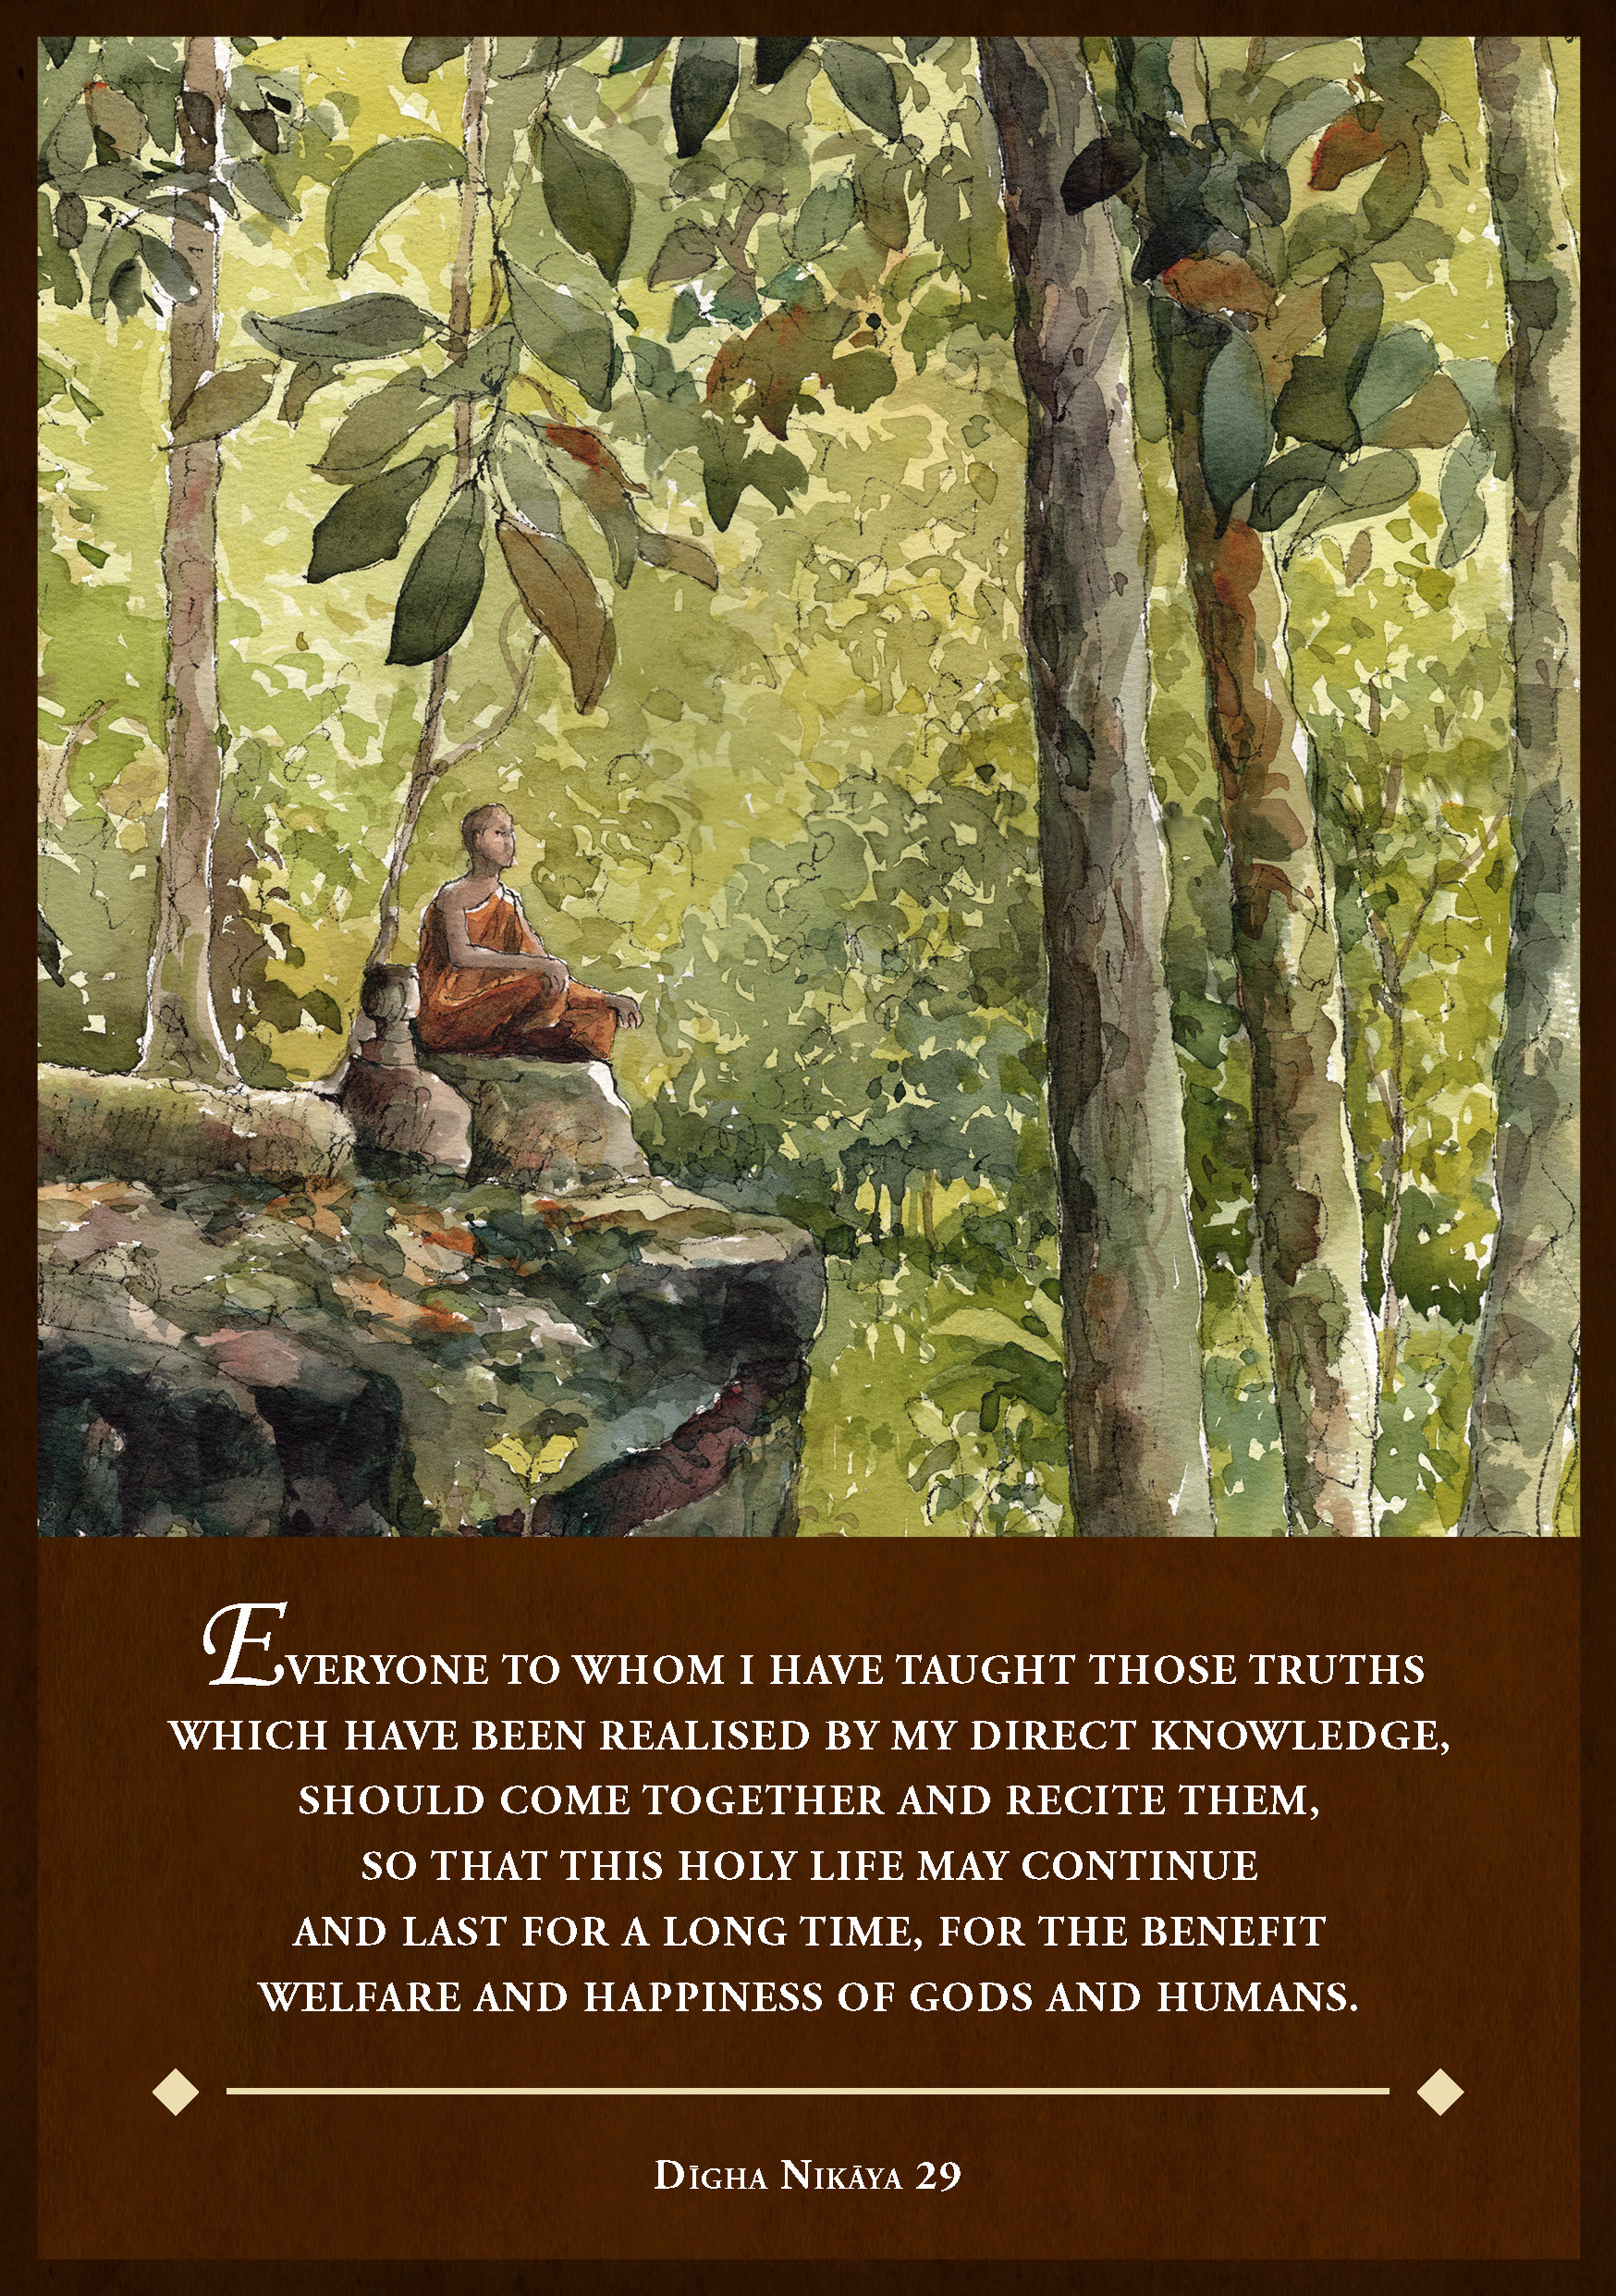
\includegraphics[height=\paperheight]{./assets/images/A5/back_cover_compressed_A5.jpg}}
\fi

\ifninebythirteenversion
  \photoFullBleed{./assets/images/9x13/back_cover_9x13.png}
\fi

\ifbfiveversion
  \photoFullBleed{./assets/images/B5/back_cover_B5.png}
\fi

\end{document}
'
% Possible VALUE:
%   - afiveVersion —  A5 formatted
%   - ninebythirteenVersion —  9x13cm custom formatted
%   - bfiveVersion —  B5 formatted
% \listfiles
\ifdefined\papersizeoption
\else
  \newcommand{\papersizeoption}{bfiveVersion}
\fi
\typeout{Set \protect\papersizeoption{} to \papersizeoption}

% Add hyperlinks and images, to be used with afiveVersion \papersizeoption
% Build command:
% '\newcommand{\papersizeoption}{afiveVersion}\newcommand{\isdigitalversion}{}% Set paper variant
% Build command '\newcommand{\papersizeoption}{VALUE}% Set paper variant
% Build command '\newcommand{\papersizeoption}{VALUE}\input{main.tex}'
% Possible VALUE:
%   - afiveVersion —  A5 formatted
%   - ninebythirteenVersion —  9x13cm custom formatted
%   - bfiveVersion —  B5 formatted
% \listfiles
\ifdefined\papersizeoption
\else
  \newcommand{\papersizeoption}{bfiveVersion}
\fi
\typeout{Set \protect\papersizeoption{} to \papersizeoption}

% Add hyperlinks and images, to be used with afiveVersion \papersizeoption
% Build command:
% '\newcommand{\papersizeoption}{afiveVersion}\newcommand{\isdigitalversion}{}\input{main.tex}'
\ifdefined\isdigitalversion
  \newcommand{\digitaloption}{digitalVersion}
\else
  \newcommand{\digitaloption}{}
\fi
\typeout{Set \protect\digitaloption{} to \digitaloption}

% todo ask bergen to make showtims a togglable condition for b5 and 9x13 only

\documentclass[
  final,
  babelLanguage=british,
  showtrims,
  \papersizeoption,
  \digitaloption,
]{anecdote}

% Define graphics path for images
\graphicspath{
  {./assets/images/A5}
  {./assets/images/9x13}
  {./assets/images/B5}
  {./assets/images/graphics}
}

% Loads formatting for selected ddocument class
\ifninebythirteenversion \usepackage{9x13} \fi
\ifafiveversion \usepackage{A5} \fi
\ifbfiveversion \usepackage{B5} \fi

% Set metadata for the document
\title{SBS Pāli-English Recitations}
\subtitle{Monk Training Centre}
\author{SBS Monk Training Centre}
\publisher{Sāsanārakkha Buddhist Sanctuary}
\date{2021-10-30}
\editionInfo{\textit{First Edition}, 2025} % And last edition. Don't call Pāladhammika.
\newcommand{\MyISBN}{} % default empty

\ifbfiveversion
  \renewcommand{\MyISBN}{978-629-97831-1-4}
\fi
\ifninebythirteenversion
  \renewcommand{\MyISBN}{978-629-97831-2-1}
\fi

\ISBN{\MyISBN}

% Set metadata for PDF properties
\hypersetup{
  pdftitle={\thetitle},
  pdfauthor={\theauthor},
  pdfcopyright={Copyright (C) 2025, \thePublisher},
  pdfsubject={},
  pdfkeywords={},
  pdflicenseurl={https://creativecommons.org/licenses/by-nc-nd/4.0/},
  pdfcontacturl={},
  pdflang={en},
}

% Load further packages
\RequirePackage[yyyymmdd,hhmmss]{datetime} % Adds the time to version creation

\makepagenote
\continuousnotenums % Ensure continuous endnote numbering

% Define hyphenation exceptions and corrections
\hyphenation{London re-lin-quishes de-ter-mines}

\ifdigitalversion
  \openany
\fi

% Begin document
\begin{document}

% Front matter
\frontmatter

% Digital version cover
\ifdigitalversion
	\digitalCover{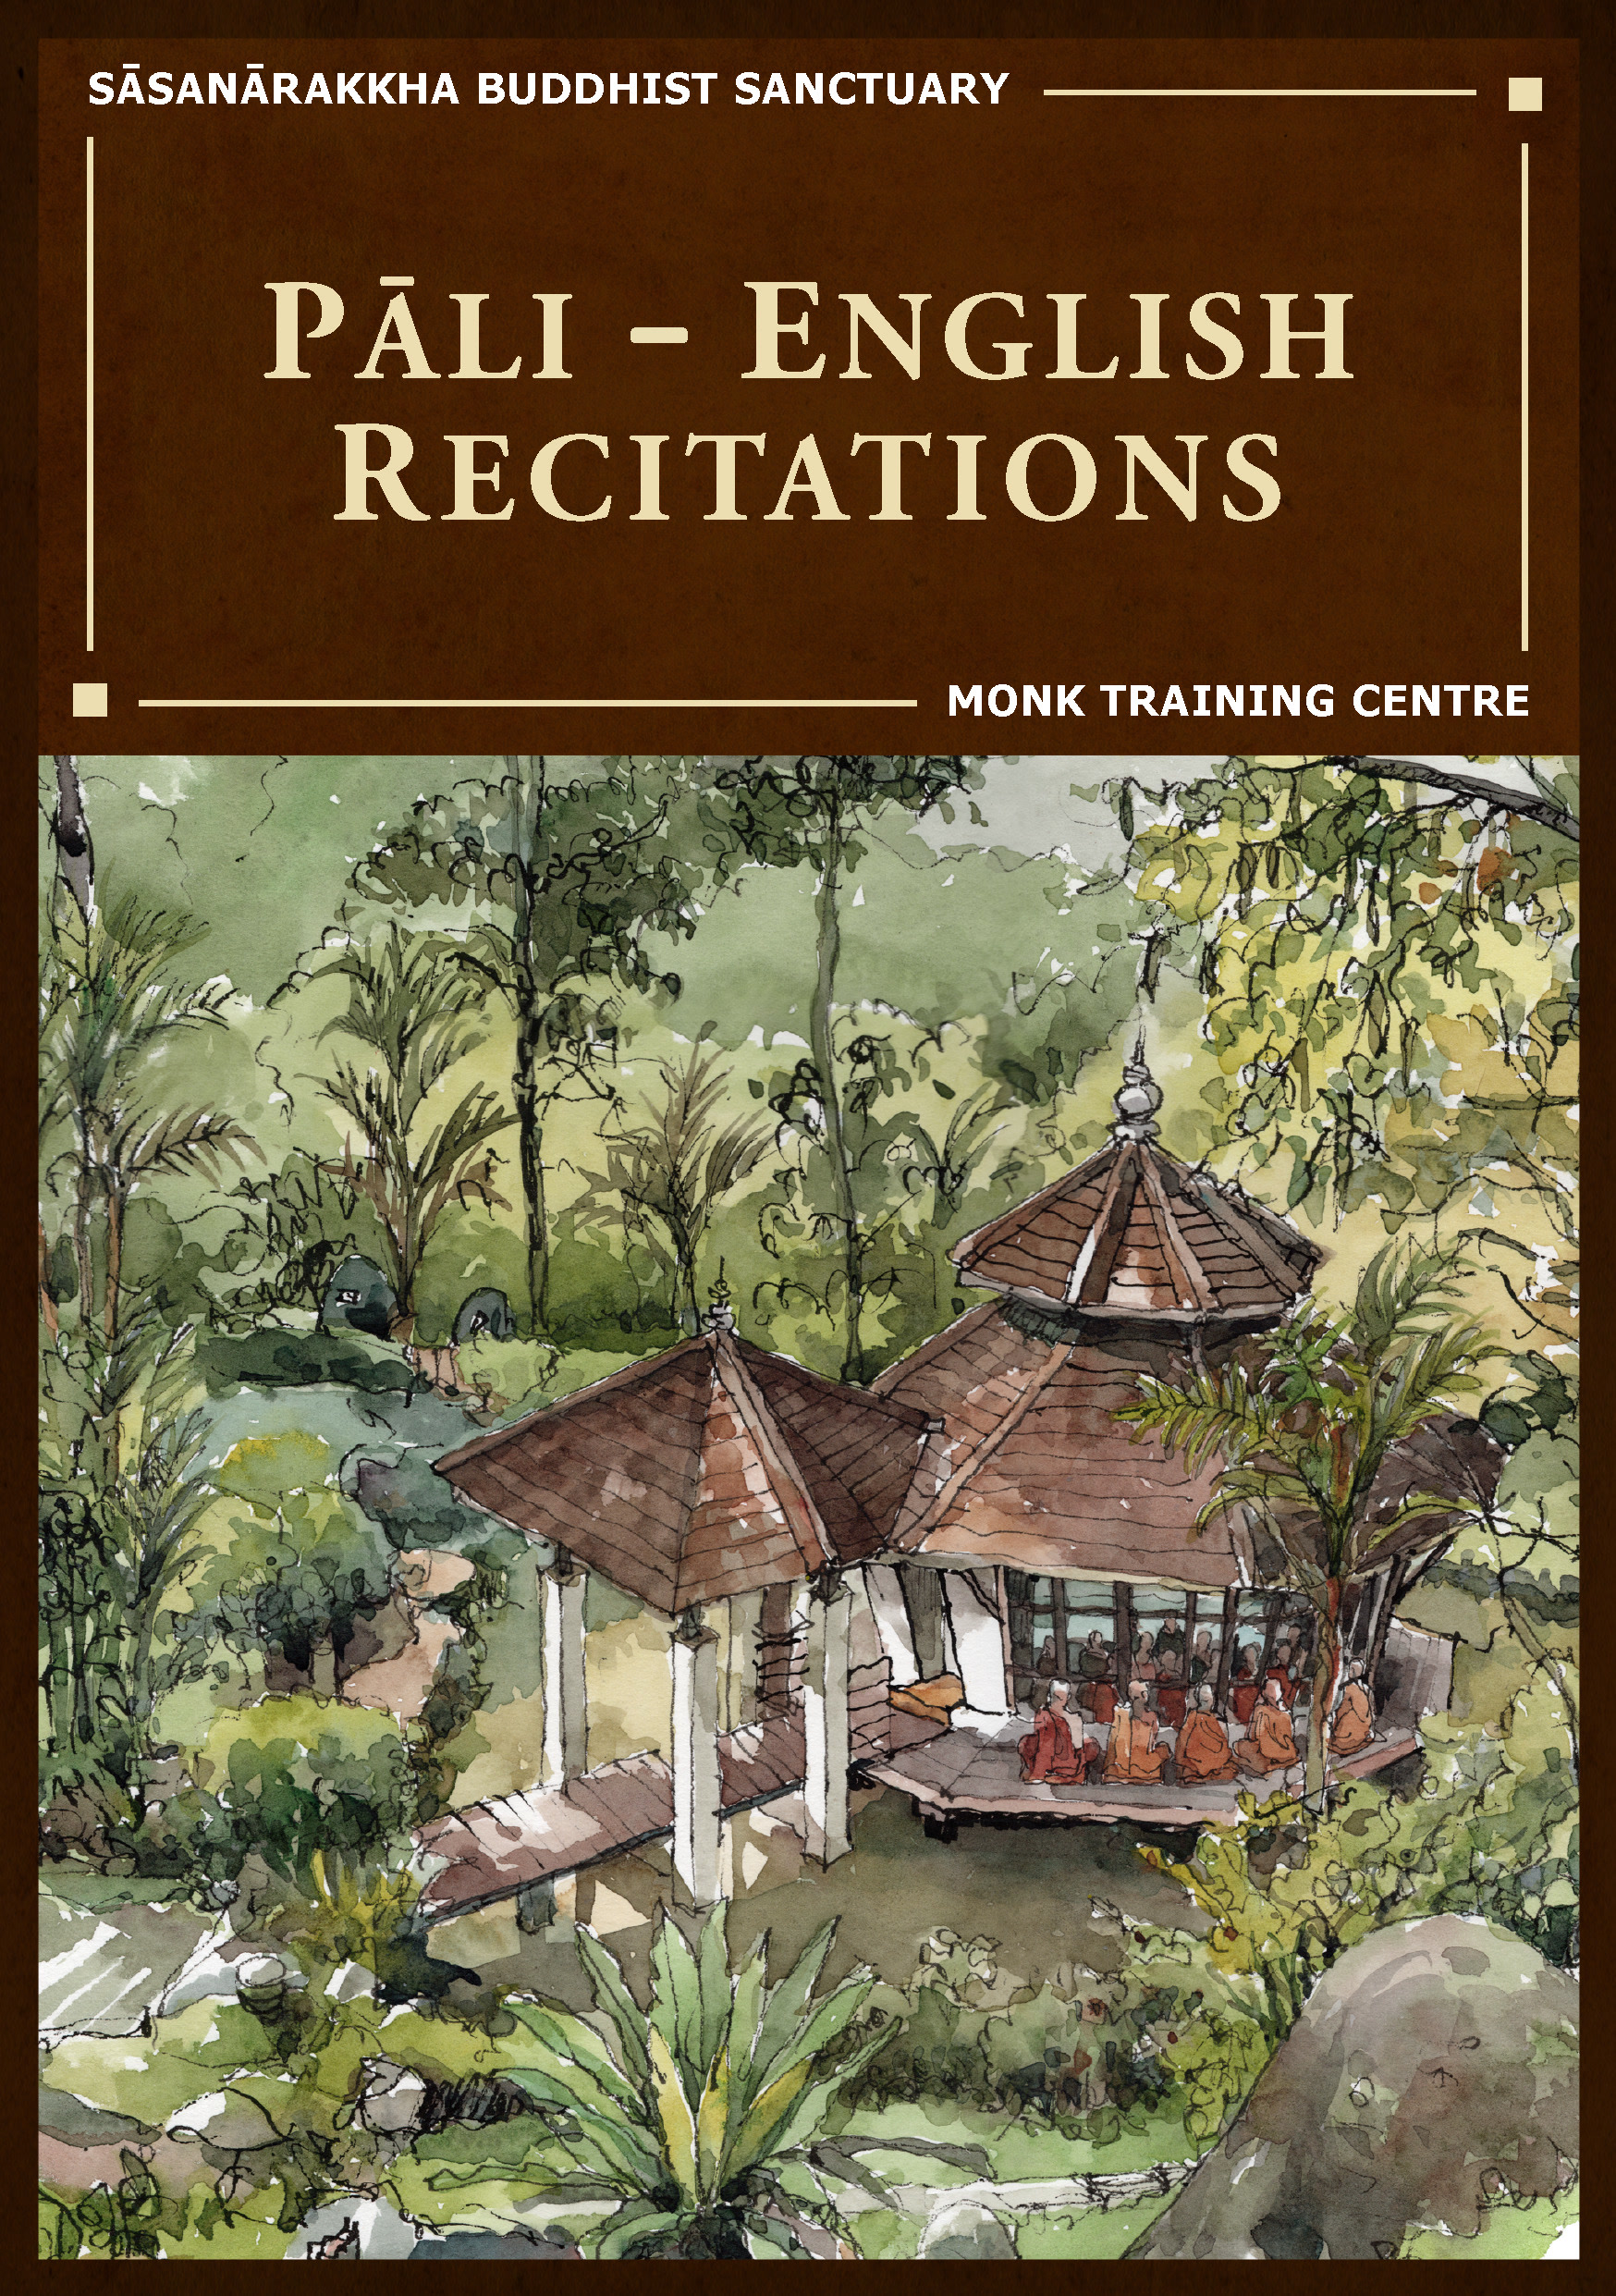
\includegraphics[height=\paperheight]{./assets/images/A5/front_cover_compressed_A5.jpg}}
\fi

\ifninebythirteenversion
  \photoFullBleed{./assets/images/9x13/front_cover_9x13.png}
  \photoFullBleed{robe_divider_left_9x13.png}
  \photoFullBleed{robe_divider_right_9x13.png}
\fi

\ifbfiveversion
  \photoFullBleed{./assets/images/B5/front_cover_B5.png}
  \photoFullBleed{robe_divider_left_B5.png}
  \photoFullBleed{robe_divider_right_B5.png}
\fi

% Title page, copyright, acknowledgments
\pagestyle{empty}
\input{./tex/titlepage.tex}
\input{./tex/copyright.tex}
\input{./tex/acknowledgments.tex}

% Table of contents, schedule, purpose and benefits, abbreviations
\cleartorecto
\pagestyle{toponerow-frontmatter}
\chapterstyle{adrasteia-toc}

\pdfbookmark[section]{\contentsname}{toc}
\tableofcontents*

\input{./tex/schedule.tex}
\input{./tex/purpose-and-benefits.tex}
\input{./tex/abbreviations.tex}

\chapterstyle{adrasteia-frontmatter}

% Main matter
\mainmatter
\pagestyle{toponerow}

\cleartorecto

% Chapters
{\raggedright
	\input{./tex/recitations/homage.tex}
	\input{./tex/recitations/verses.tex}
	\input{./tex/recitations/teachings.tex}
	\input{./tex/recitations/reflections.tex}
	\input{./tex/recitations/cardinal-discourses.tex}
	\input{./tex/recitations/thanksgiving-recitations.tex}
	\input{./tex/recitations/protective-recitations.tex}
	\input{./tex/recitations/funeral-recitations.tex}
	\input{./tex/recitations/sharing-of-merits.tex}
}

% Appendix
\appendix
\input{./tex/appendix.tex}
\input{./tex/refuge-trainings.tex}
\input{./tex/phonetics-pronunciation.tex}
\input{./tex/guidelines.tex}

% Back matter
\backmatter
\printpagenotes % Print endnotes
\input{./tex/copyright-details.tex}

\ifbfiveversion
  \includepdf[pages=-,pagecommand={\thispagestyle{empty}}]{assets/images/graphics/donor-list.pdf}
  \photoFullBleed{robe_divider_left_B5.png}
  \photoFullBleed{robe_divider_right_B5.png}
\fi

\ifninebythirteenversion
  \photoFullBleed{robe_divider_left_9x13.png}
  \photoFullBleed{robe_divider_right_9x13.png}
\fi

\emptyUntilEven % Add blank page if necessary

\ifdigitalversion
  \clearpage
  \digitalCover{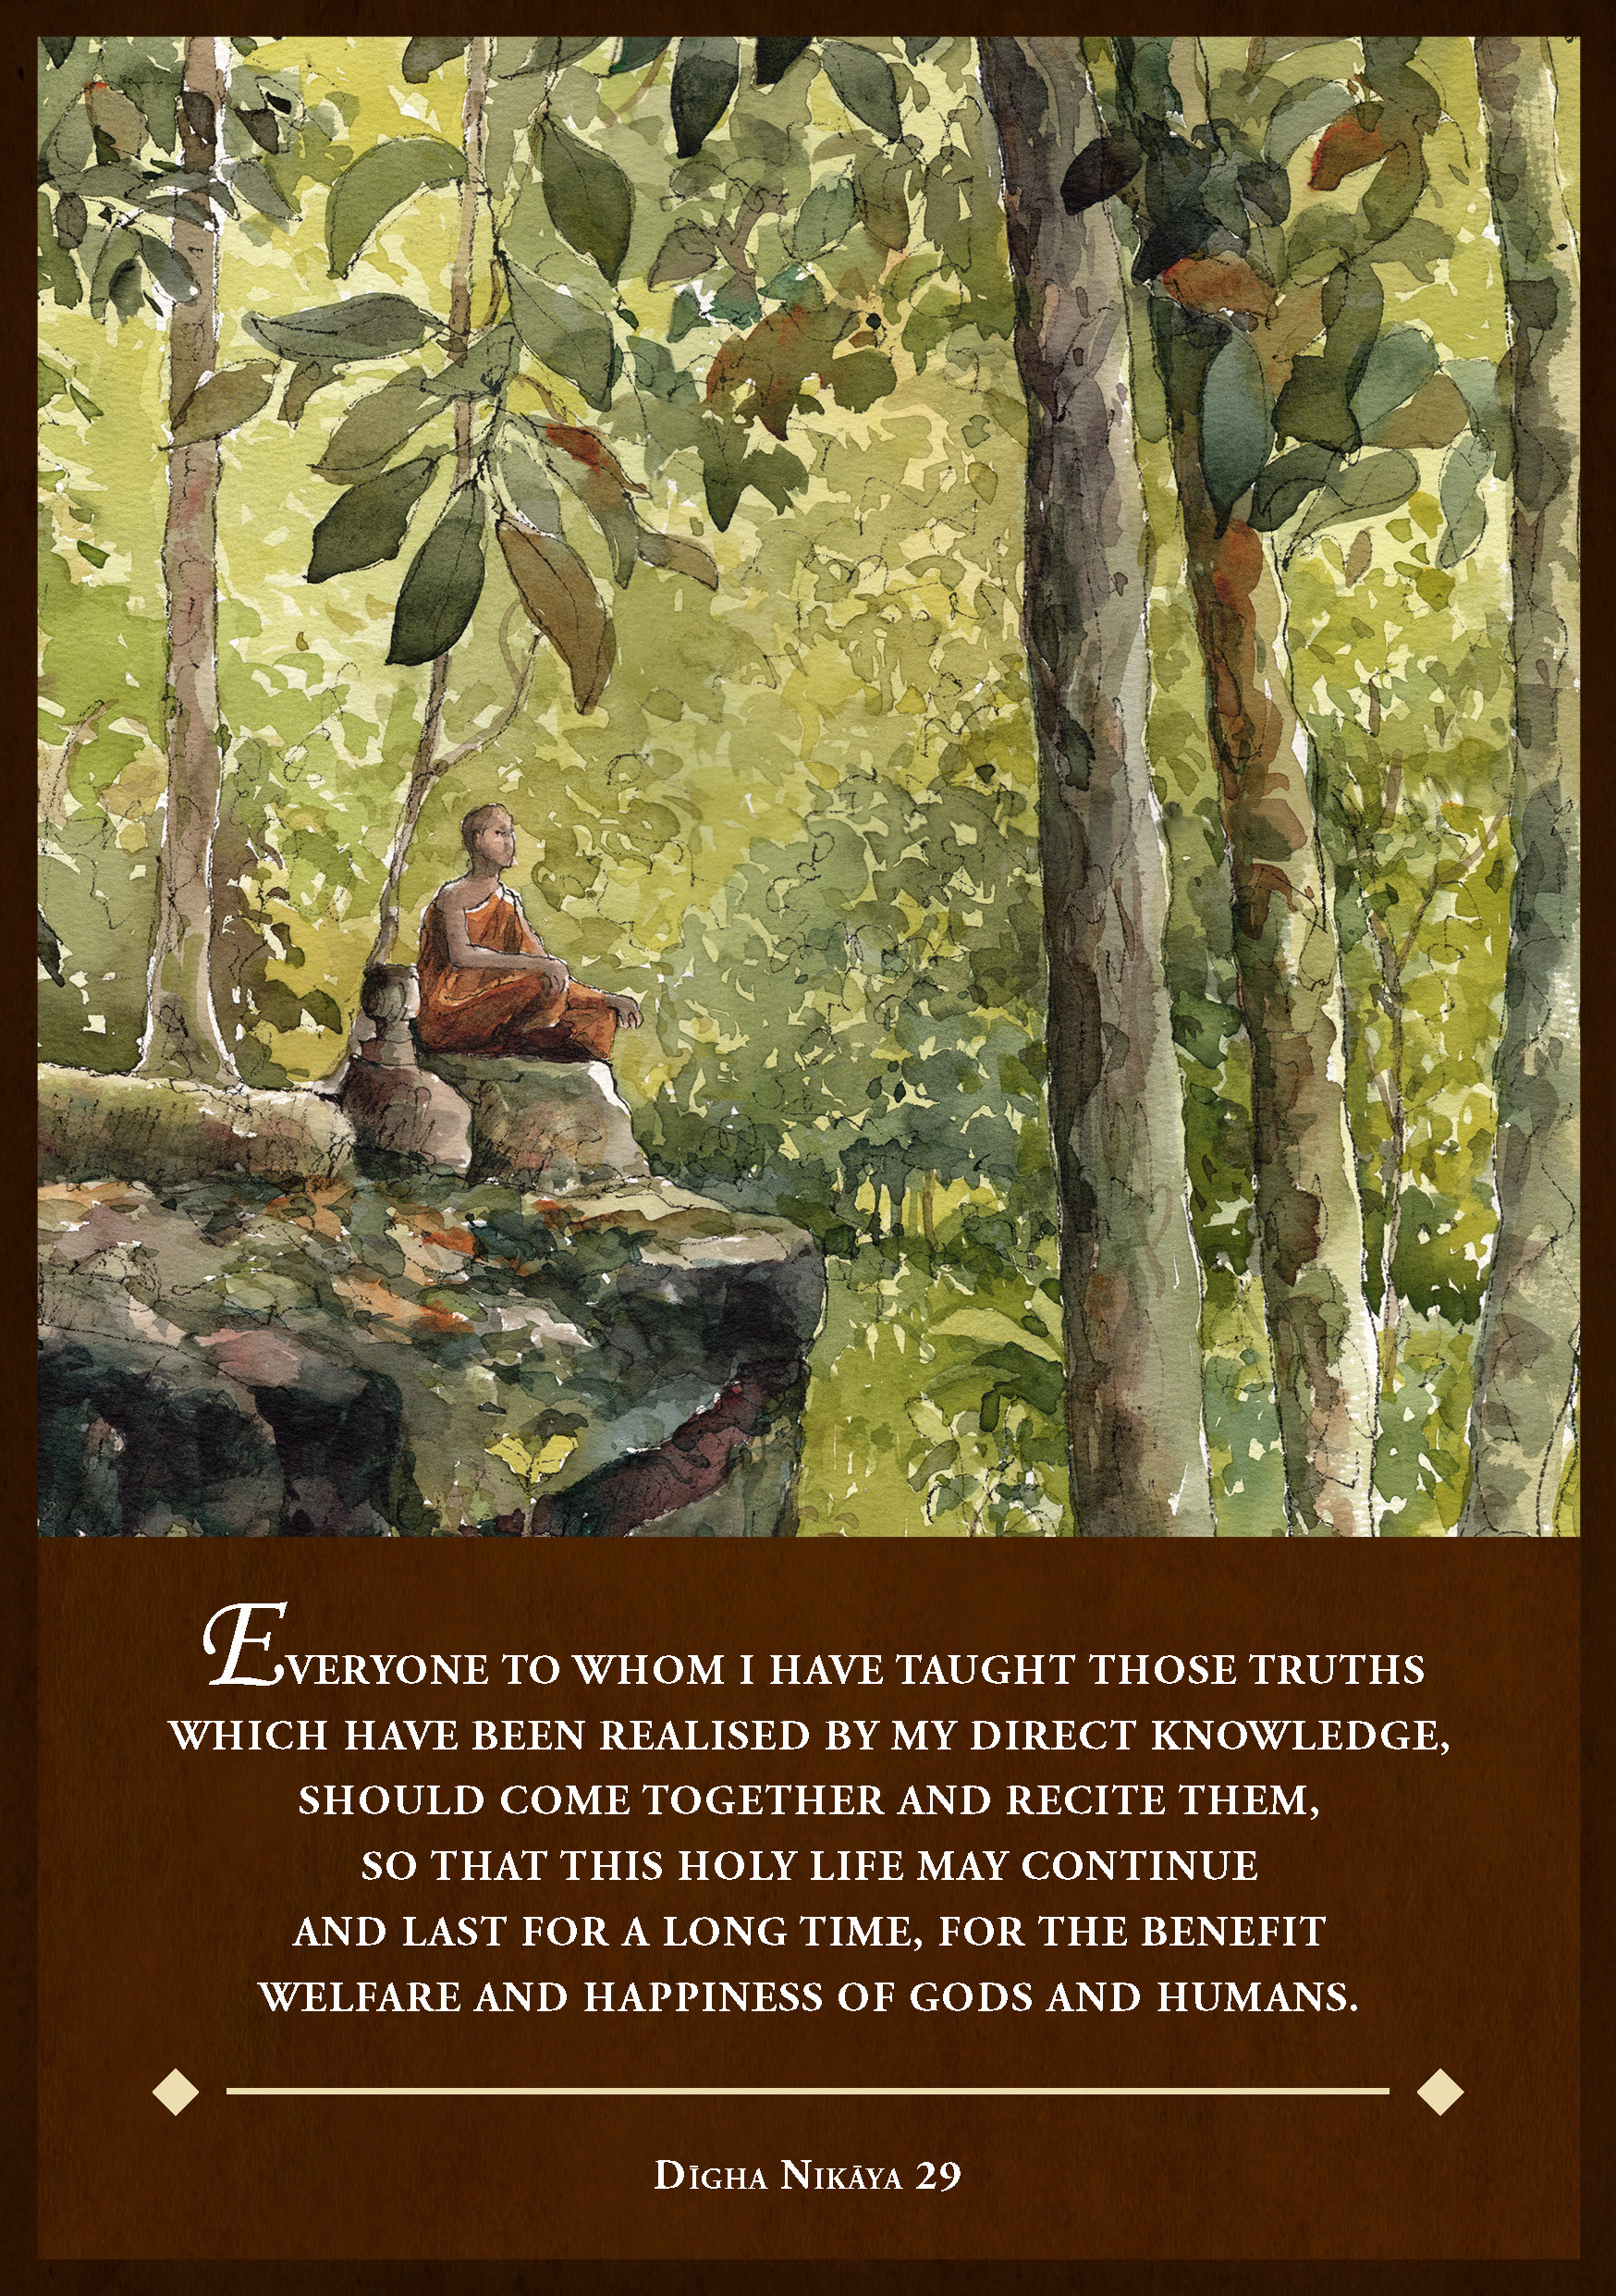
\includegraphics[height=\paperheight]{./assets/images/A5/back_cover_compressed_A5.jpg}}
\fi

\ifninebythirteenversion
  \photoFullBleed{./assets/images/9x13/back_cover_9x13.png}
\fi

\ifbfiveversion
  \photoFullBleed{./assets/images/B5/back_cover_B5.png}
\fi

\end{document}
'
% Possible VALUE:
%   - afiveVersion —  A5 formatted
%   - ninebythirteenVersion —  9x13cm custom formatted
%   - bfiveVersion —  B5 formatted
% \listfiles
\ifdefined\papersizeoption
\else
  \newcommand{\papersizeoption}{bfiveVersion}
\fi
\typeout{Set \protect\papersizeoption{} to \papersizeoption}

% Add hyperlinks and images, to be used with afiveVersion \papersizeoption
% Build command:
% '\newcommand{\papersizeoption}{afiveVersion}\newcommand{\isdigitalversion}{}% Set paper variant
% Build command '\newcommand{\papersizeoption}{VALUE}\input{main.tex}'
% Possible VALUE:
%   - afiveVersion —  A5 formatted
%   - ninebythirteenVersion —  9x13cm custom formatted
%   - bfiveVersion —  B5 formatted
% \listfiles
\ifdefined\papersizeoption
\else
  \newcommand{\papersizeoption}{bfiveVersion}
\fi
\typeout{Set \protect\papersizeoption{} to \papersizeoption}

% Add hyperlinks and images, to be used with afiveVersion \papersizeoption
% Build command:
% '\newcommand{\papersizeoption}{afiveVersion}\newcommand{\isdigitalversion}{}\input{main.tex}'
\ifdefined\isdigitalversion
  \newcommand{\digitaloption}{digitalVersion}
\else
  \newcommand{\digitaloption}{}
\fi
\typeout{Set \protect\digitaloption{} to \digitaloption}

% todo ask bergen to make showtims a togglable condition for b5 and 9x13 only

\documentclass[
  final,
  babelLanguage=british,
  showtrims,
  \papersizeoption,
  \digitaloption,
]{anecdote}

% Define graphics path for images
\graphicspath{
  {./assets/images/A5}
  {./assets/images/9x13}
  {./assets/images/B5}
  {./assets/images/graphics}
}

% Loads formatting for selected ddocument class
\ifninebythirteenversion \usepackage{9x13} \fi
\ifafiveversion \usepackage{A5} \fi
\ifbfiveversion \usepackage{B5} \fi

% Set metadata for the document
\title{SBS Pāli-English Recitations}
\subtitle{Monk Training Centre}
\author{SBS Monk Training Centre}
\publisher{Sāsanārakkha Buddhist Sanctuary}
\date{2021-10-30}
\editionInfo{\textit{First Edition}, 2025} % And last edition. Don't call Pāladhammika.
\newcommand{\MyISBN}{} % default empty

\ifbfiveversion
  \renewcommand{\MyISBN}{978-629-97831-1-4}
\fi
\ifninebythirteenversion
  \renewcommand{\MyISBN}{978-629-97831-2-1}
\fi

\ISBN{\MyISBN}

% Set metadata for PDF properties
\hypersetup{
  pdftitle={\thetitle},
  pdfauthor={\theauthor},
  pdfcopyright={Copyright (C) 2025, \thePublisher},
  pdfsubject={},
  pdfkeywords={},
  pdflicenseurl={https://creativecommons.org/licenses/by-nc-nd/4.0/},
  pdfcontacturl={},
  pdflang={en},
}

% Load further packages
\RequirePackage[yyyymmdd,hhmmss]{datetime} % Adds the time to version creation

\makepagenote
\continuousnotenums % Ensure continuous endnote numbering

% Define hyphenation exceptions and corrections
\hyphenation{London re-lin-quishes de-ter-mines}

\ifdigitalversion
  \openany
\fi

% Begin document
\begin{document}

% Front matter
\frontmatter

% Digital version cover
\ifdigitalversion
	\digitalCover{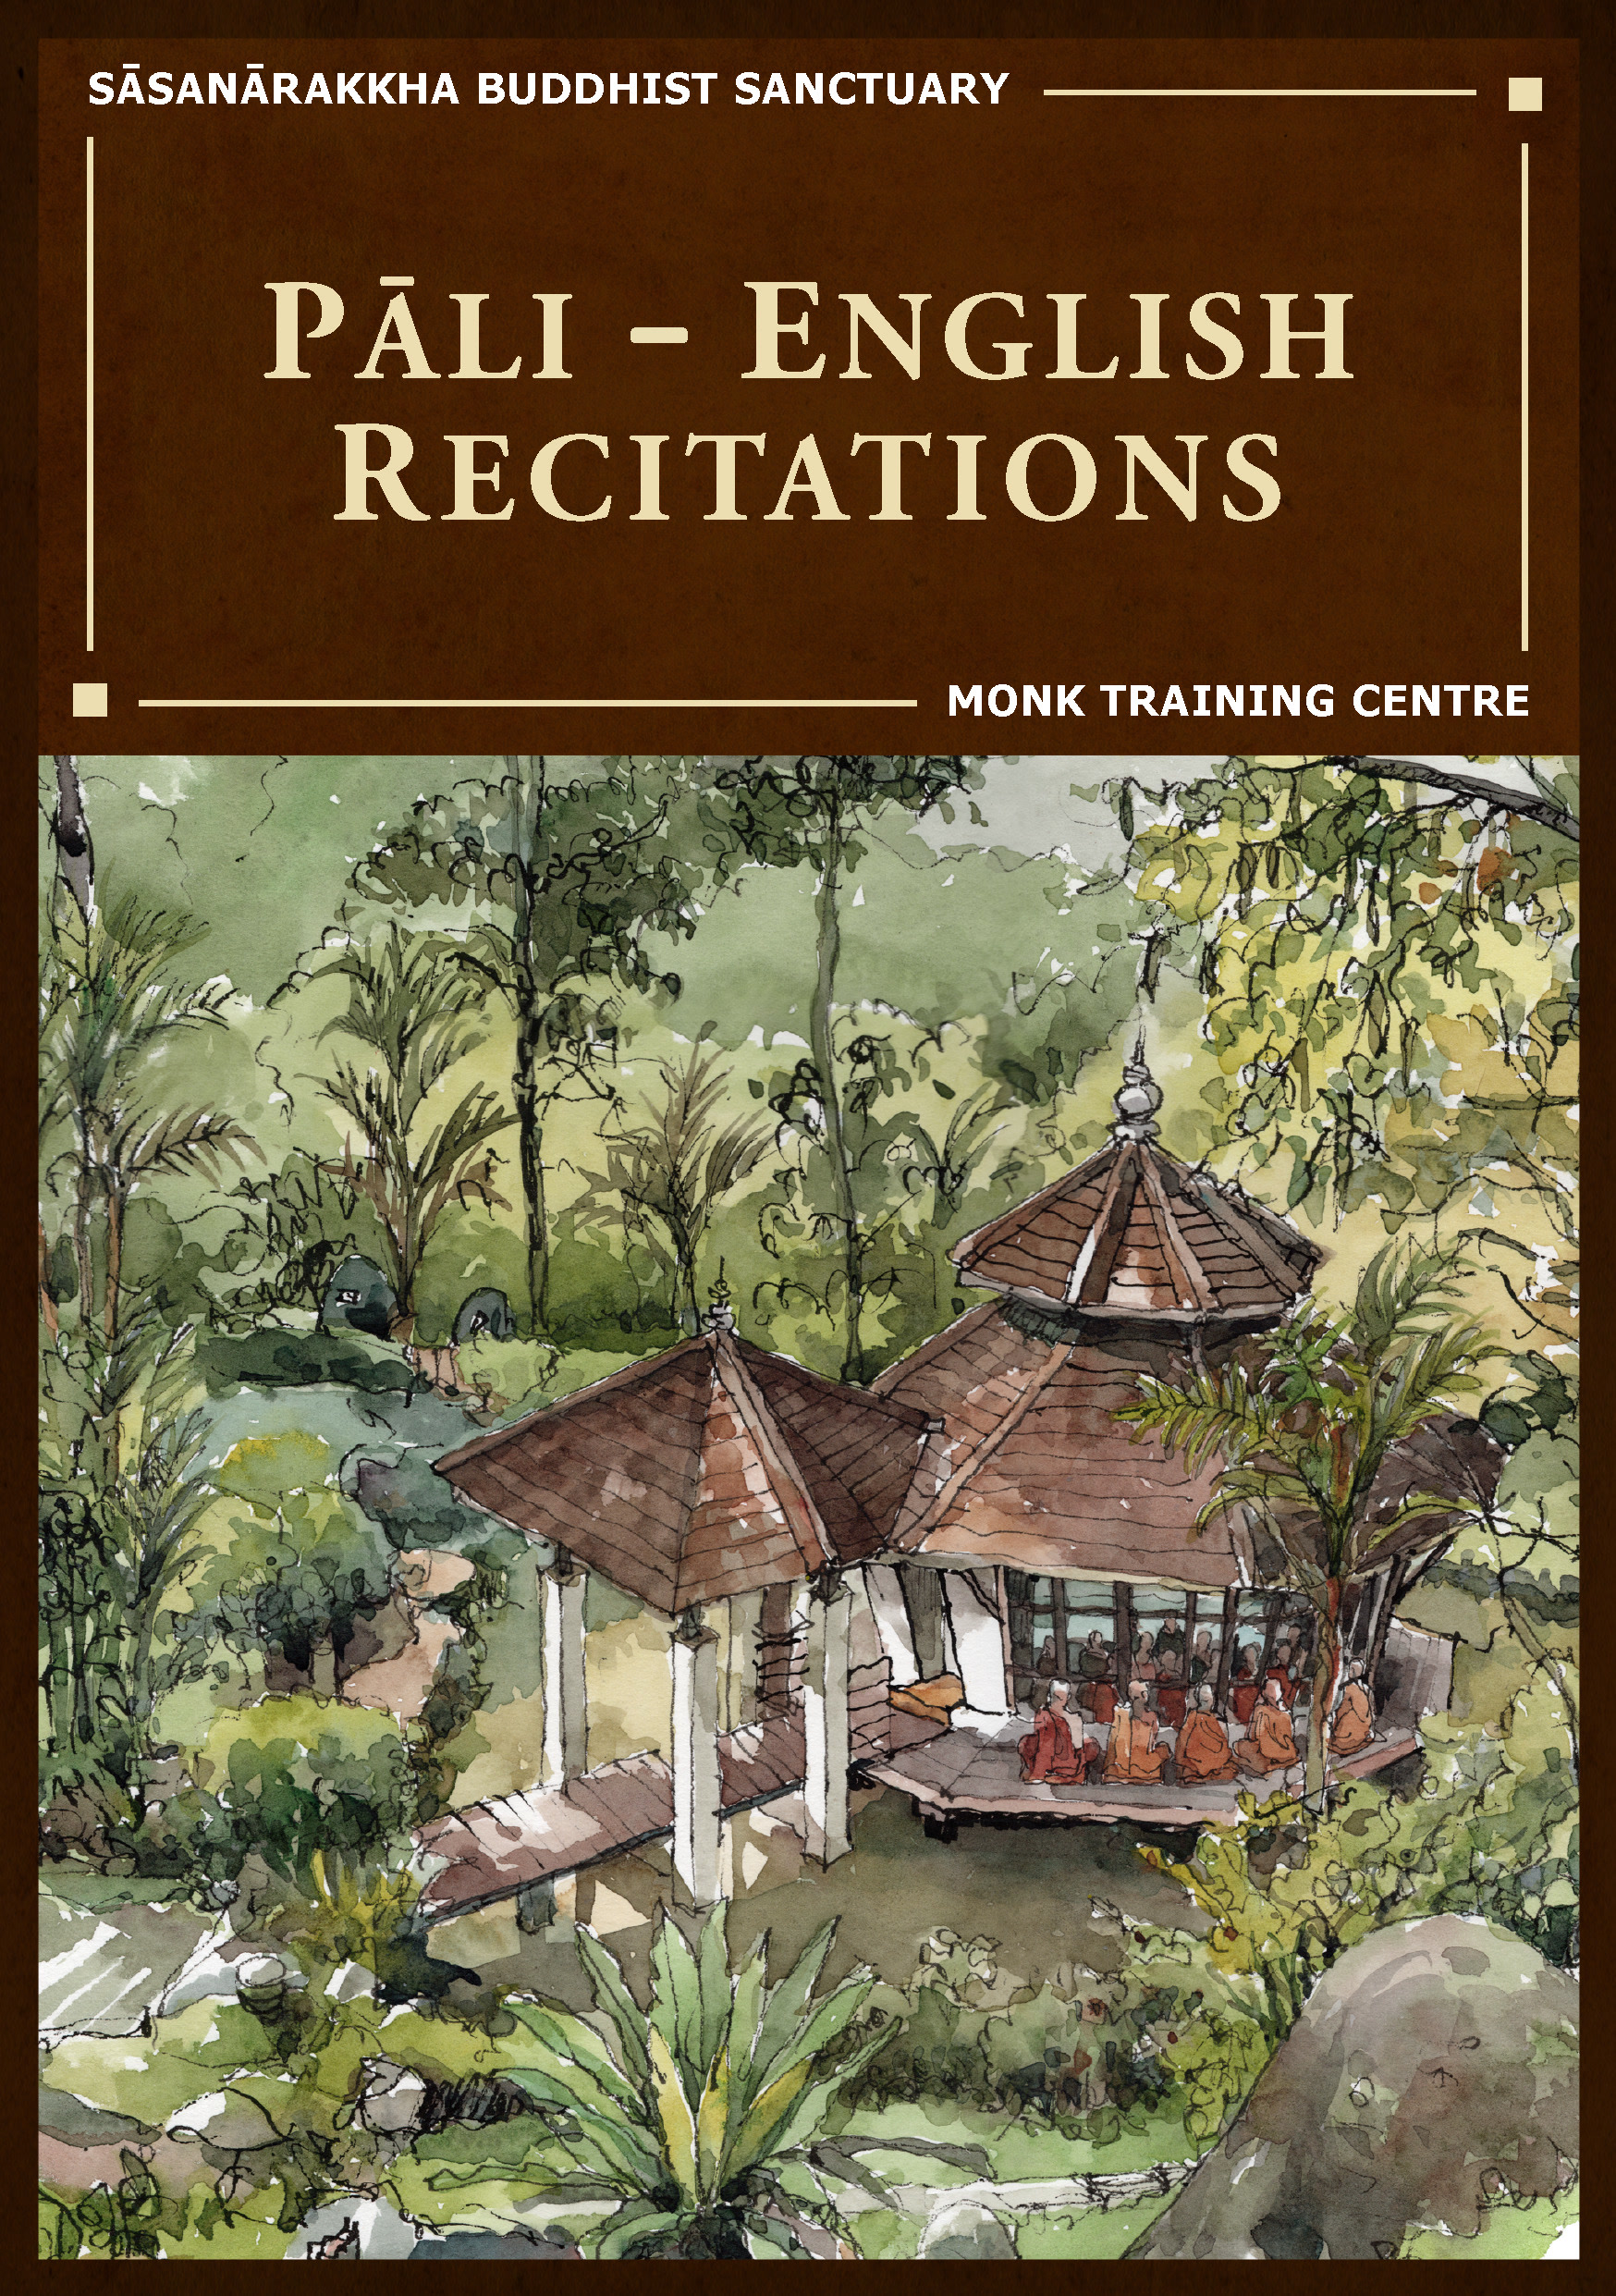
\includegraphics[height=\paperheight]{./assets/images/A5/front_cover_compressed_A5.jpg}}
\fi

\ifninebythirteenversion
  \photoFullBleed{./assets/images/9x13/front_cover_9x13.png}
  \photoFullBleed{robe_divider_left_9x13.png}
  \photoFullBleed{robe_divider_right_9x13.png}
\fi

\ifbfiveversion
  \photoFullBleed{./assets/images/B5/front_cover_B5.png}
  \photoFullBleed{robe_divider_left_B5.png}
  \photoFullBleed{robe_divider_right_B5.png}
\fi

% Title page, copyright, acknowledgments
\pagestyle{empty}
\input{./tex/titlepage.tex}
\input{./tex/copyright.tex}
\input{./tex/acknowledgments.tex}

% Table of contents, schedule, purpose and benefits, abbreviations
\cleartorecto
\pagestyle{toponerow-frontmatter}
\chapterstyle{adrasteia-toc}

\pdfbookmark[section]{\contentsname}{toc}
\tableofcontents*

\input{./tex/schedule.tex}
\input{./tex/purpose-and-benefits.tex}
\input{./tex/abbreviations.tex}

\chapterstyle{adrasteia-frontmatter}

% Main matter
\mainmatter
\pagestyle{toponerow}

\cleartorecto

% Chapters
{\raggedright
	\input{./tex/recitations/homage.tex}
	\input{./tex/recitations/verses.tex}
	\input{./tex/recitations/teachings.tex}
	\input{./tex/recitations/reflections.tex}
	\input{./tex/recitations/cardinal-discourses.tex}
	\input{./tex/recitations/thanksgiving-recitations.tex}
	\input{./tex/recitations/protective-recitations.tex}
	\input{./tex/recitations/funeral-recitations.tex}
	\input{./tex/recitations/sharing-of-merits.tex}
}

% Appendix
\appendix
\input{./tex/appendix.tex}
\input{./tex/refuge-trainings.tex}
\input{./tex/phonetics-pronunciation.tex}
\input{./tex/guidelines.tex}

% Back matter
\backmatter
\printpagenotes % Print endnotes
\input{./tex/copyright-details.tex}

\ifbfiveversion
  \includepdf[pages=-,pagecommand={\thispagestyle{empty}}]{assets/images/graphics/donor-list.pdf}
  \photoFullBleed{robe_divider_left_B5.png}
  \photoFullBleed{robe_divider_right_B5.png}
\fi

\ifninebythirteenversion
  \photoFullBleed{robe_divider_left_9x13.png}
  \photoFullBleed{robe_divider_right_9x13.png}
\fi

\emptyUntilEven % Add blank page if necessary

\ifdigitalversion
  \clearpage
  \digitalCover{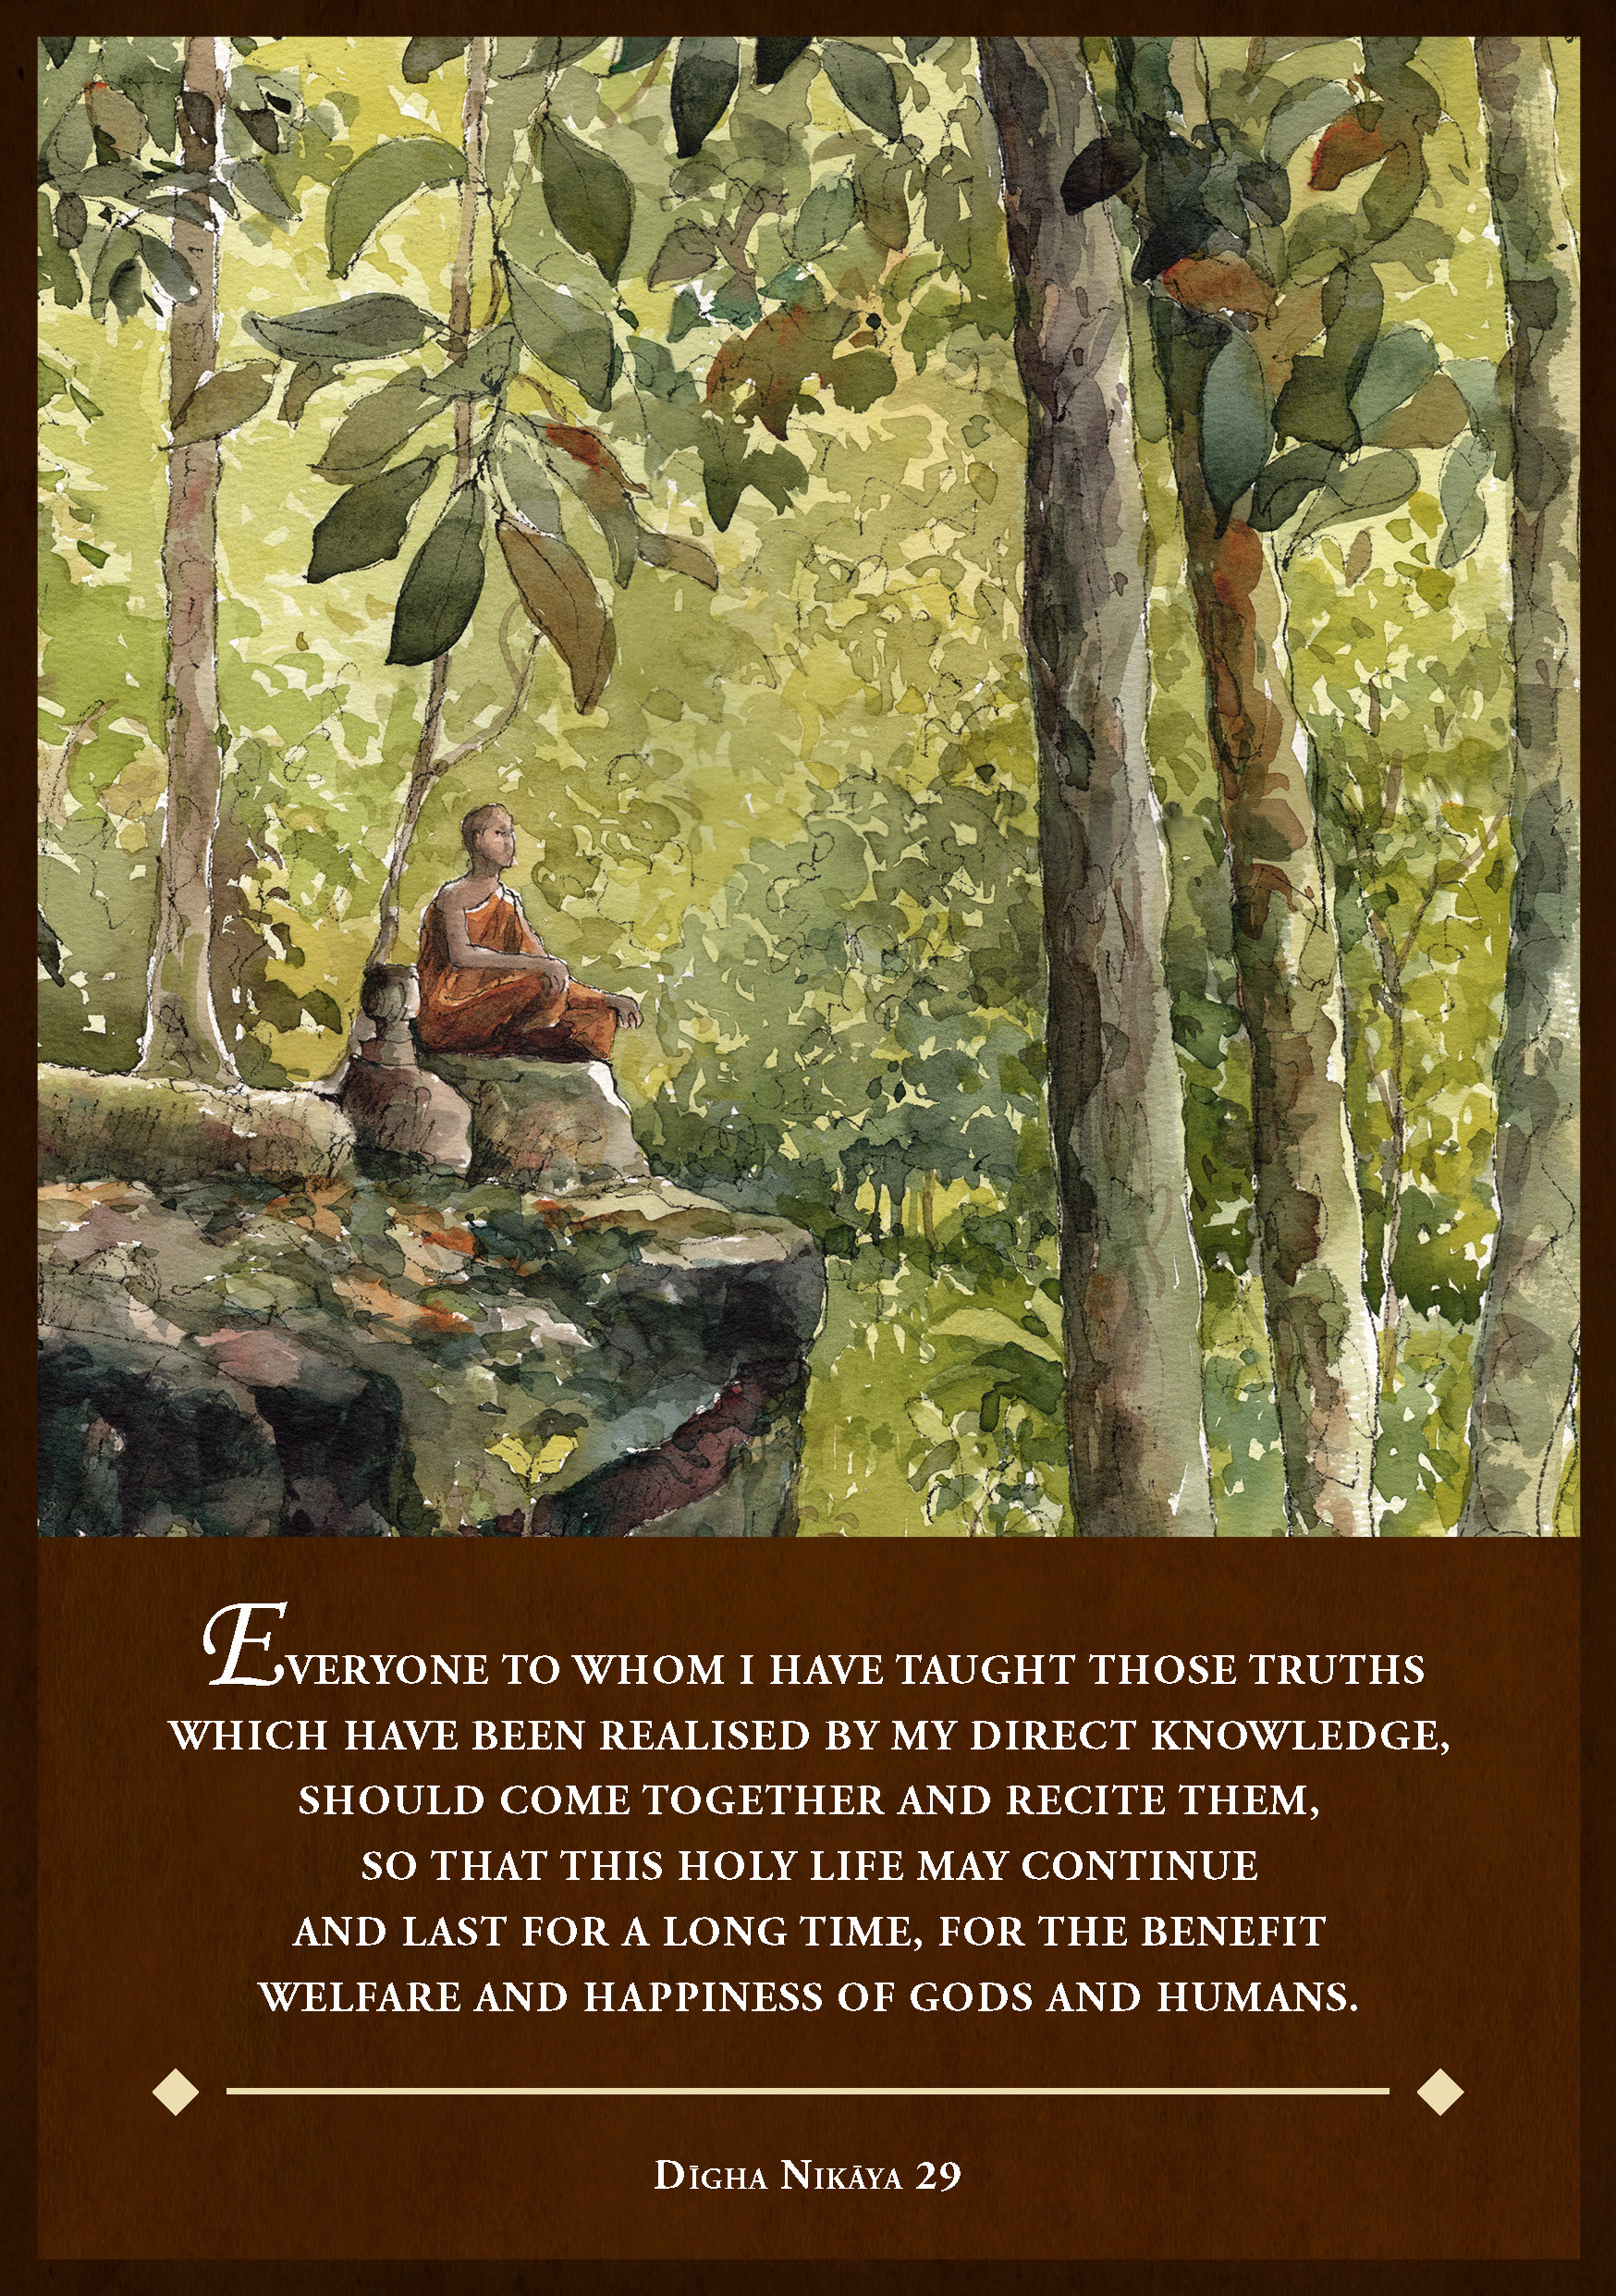
\includegraphics[height=\paperheight]{./assets/images/A5/back_cover_compressed_A5.jpg}}
\fi

\ifninebythirteenversion
  \photoFullBleed{./assets/images/9x13/back_cover_9x13.png}
\fi

\ifbfiveversion
  \photoFullBleed{./assets/images/B5/back_cover_B5.png}
\fi

\end{document}
'
\ifdefined\isdigitalversion
  \newcommand{\digitaloption}{digitalVersion}
\else
  \newcommand{\digitaloption}{}
\fi
\typeout{Set \protect\digitaloption{} to \digitaloption}

% todo ask bergen to make showtims a togglable condition for b5 and 9x13 only

\documentclass[
  final,
  babelLanguage=british,
  showtrims,
  \papersizeoption,
  \digitaloption,
]{anecdote}

% Define graphics path for images
\graphicspath{
  {./assets/images/A5}
  {./assets/images/9x13}
  {./assets/images/B5}
  {./assets/images/graphics}
}

% Loads formatting for selected ddocument class
\ifninebythirteenversion \usepackage{9x13} \fi
\ifafiveversion \usepackage{A5} \fi
\ifbfiveversion \usepackage{B5} \fi

% Set metadata for the document
\title{SBS Pāli-English Recitations}
\subtitle{Monk Training Centre}
\author{SBS Monk Training Centre}
\publisher{Sāsanārakkha Buddhist Sanctuary}
\date{2021-10-30}
\editionInfo{\textit{First Edition}, 2025} % And last edition. Don't call Pāladhammika.
\newcommand{\MyISBN}{} % default empty

\ifbfiveversion
  \renewcommand{\MyISBN}{978-629-97831-1-4}
\fi
\ifninebythirteenversion
  \renewcommand{\MyISBN}{978-629-97831-2-1}
\fi

\ISBN{\MyISBN}

% Set metadata for PDF properties
\hypersetup{
  pdftitle={\thetitle},
  pdfauthor={\theauthor},
  pdfcopyright={Copyright (C) 2025, \thePublisher},
  pdfsubject={},
  pdfkeywords={},
  pdflicenseurl={https://creativecommons.org/licenses/by-nc-nd/4.0/},
  pdfcontacturl={},
  pdflang={en},
}

% Load further packages
\RequirePackage[yyyymmdd,hhmmss]{datetime} % Adds the time to version creation

\makepagenote
\continuousnotenums % Ensure continuous endnote numbering

% Define hyphenation exceptions and corrections
\hyphenation{London re-lin-quishes de-ter-mines}

\ifdigitalversion
  \openany
\fi

% Begin document
\begin{document}

% Front matter
\frontmatter

% Digital version cover
\ifdigitalversion
	\digitalCover{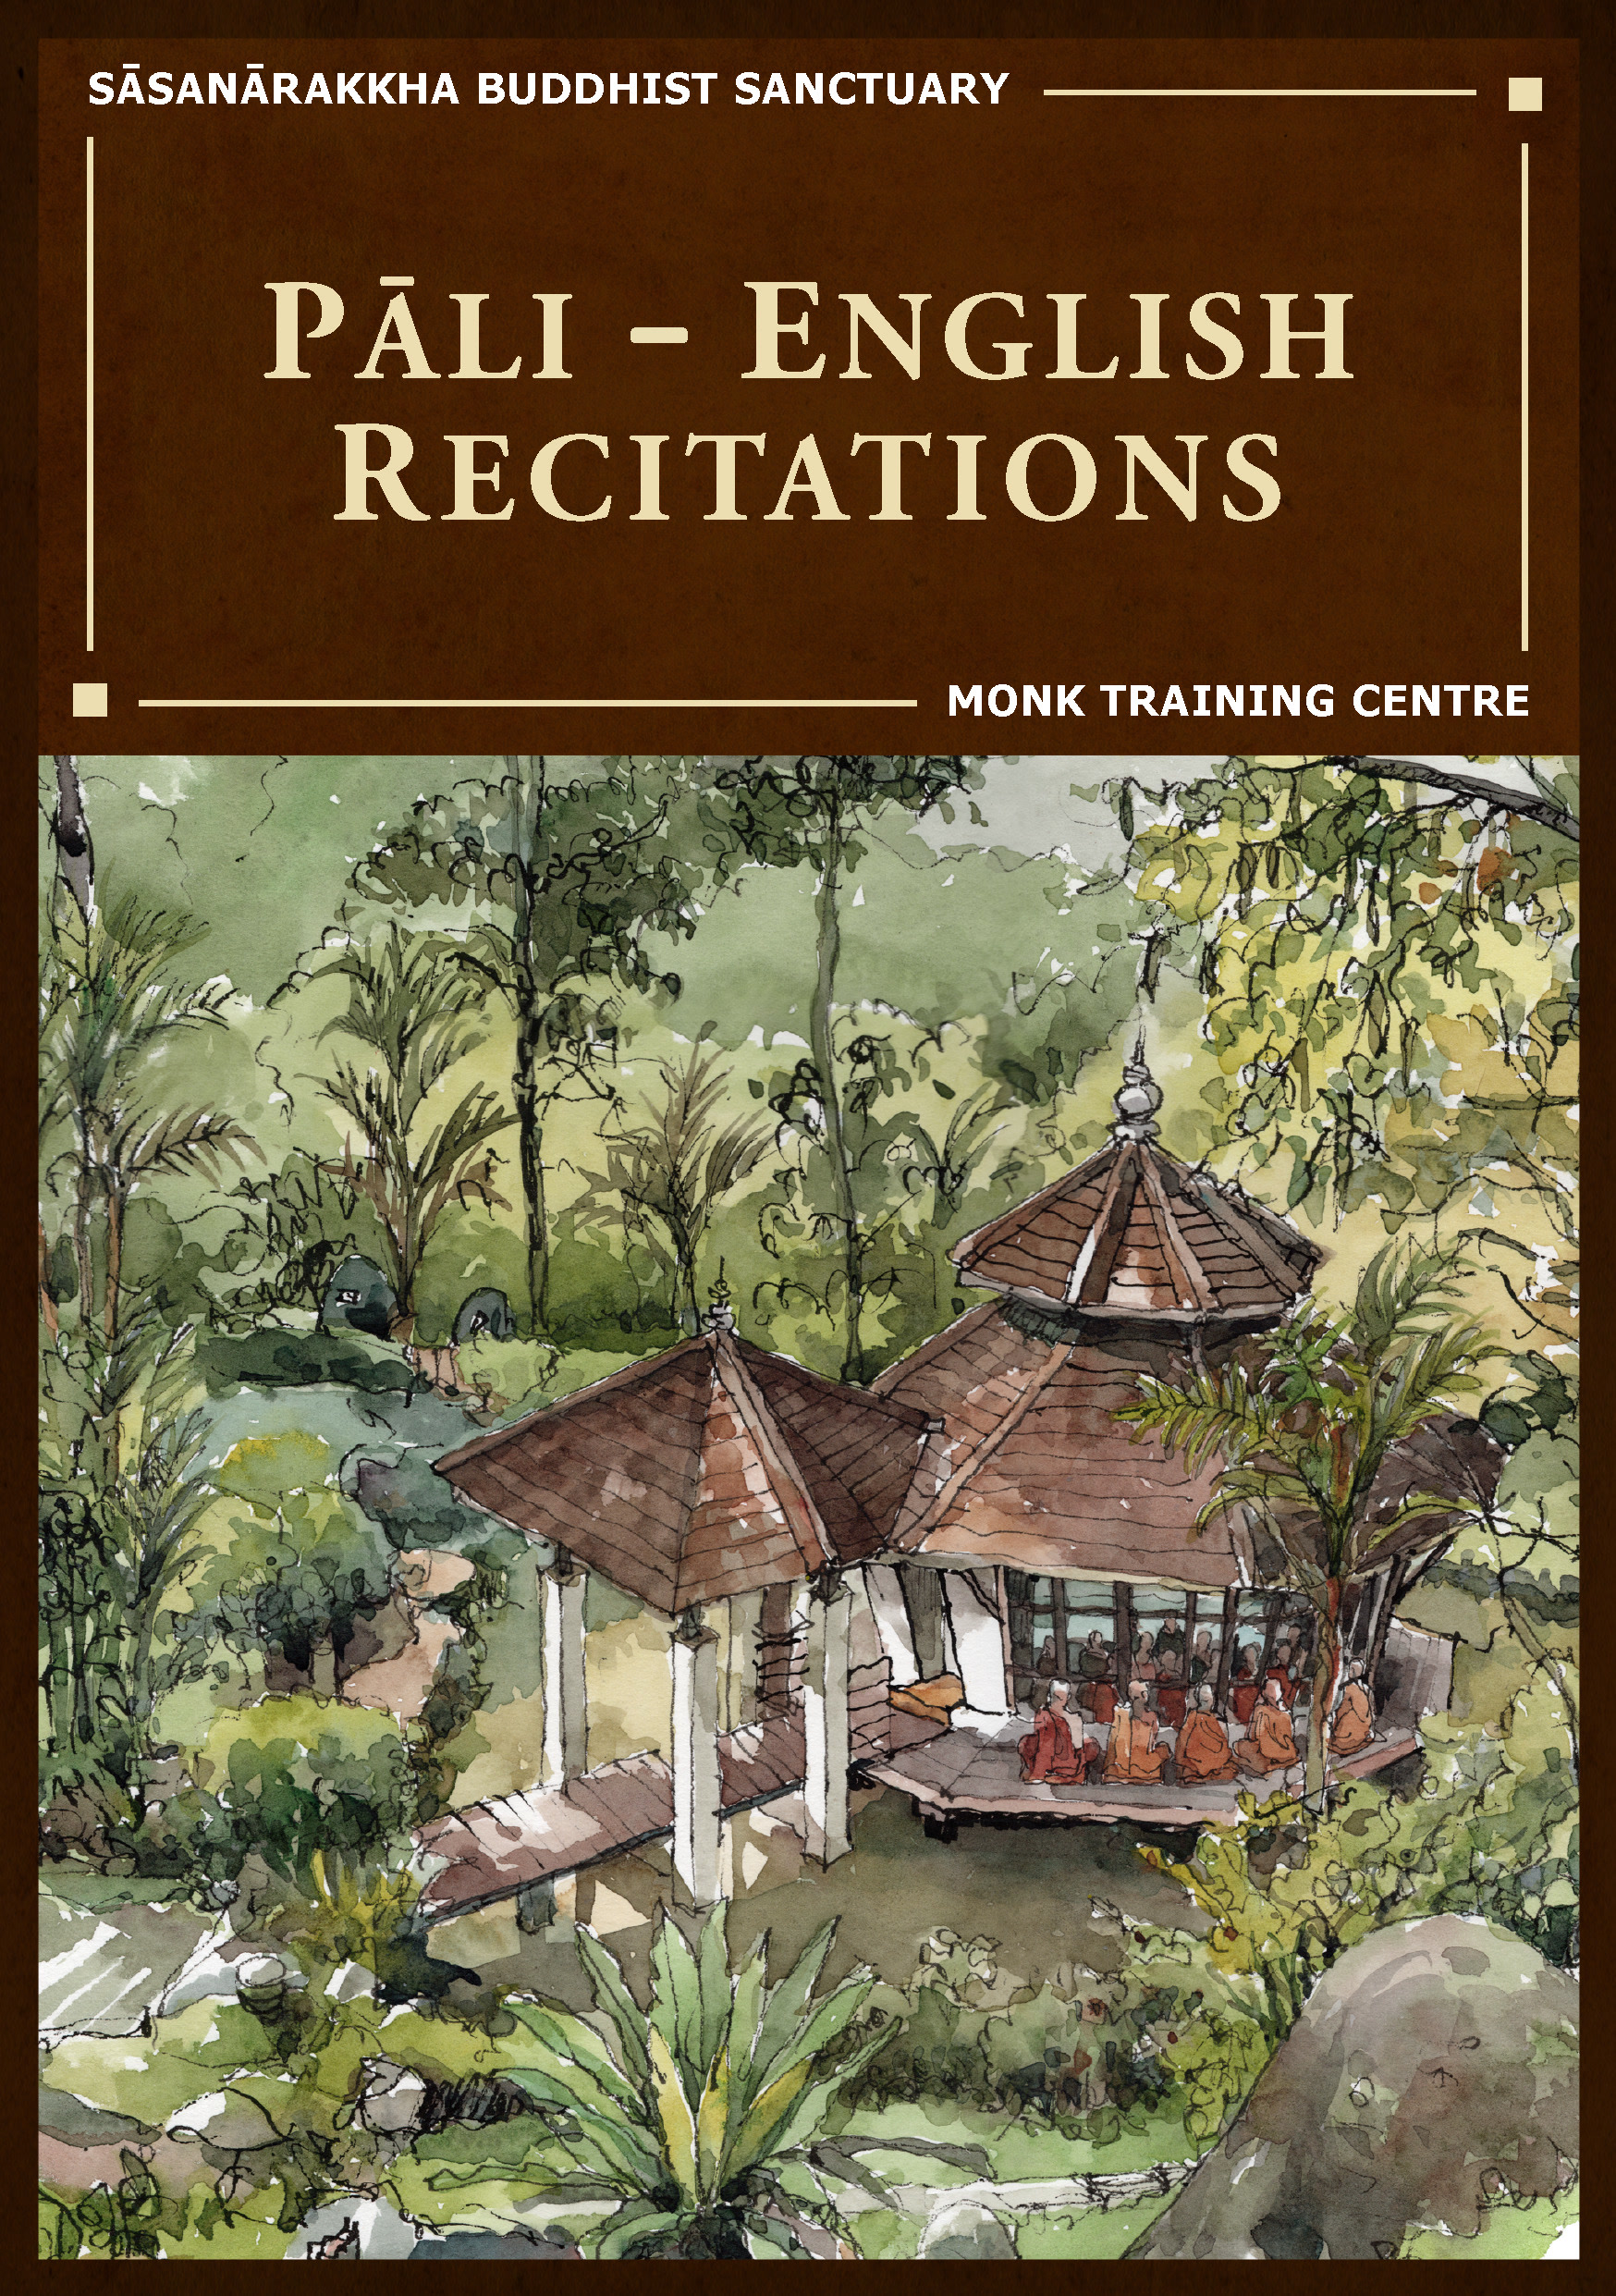
\includegraphics[height=\paperheight]{./assets/images/A5/front_cover_compressed_A5.jpg}}
\fi

\ifninebythirteenversion
  \photoFullBleed{./assets/images/9x13/front_cover_9x13.png}
  \photoFullBleed{robe_divider_left_9x13.png}
  \photoFullBleed{robe_divider_right_9x13.png}
\fi

\ifbfiveversion
  \photoFullBleed{./assets/images/B5/front_cover_B5.png}
  \photoFullBleed{robe_divider_left_B5.png}
  \photoFullBleed{robe_divider_right_B5.png}
\fi

% Title page, copyright, acknowledgments
\pagestyle{empty}

\cleartorecto
\thispagestyle{empty}

\vspace*{3em}

{\centering

  \settowidth{\titleLength}{%
    {\Large\chapterTitleFont\textsc{\MakeUppercase{{Pāli-English Recitations}}}}%
  }

  % 'SBS' on title page
  \ifafive {\Huge\fontsize{64}{16}\sbsFont SBS}\\[1.0\baselineskip] \fi
  \ifninebythirteen {\Huge\fontsize{42.5}{11}\sbsFont SBS}\\[1.0\baselineskip] \fi
  \ifbfive {\Huge\fontsize{80}{16}\sbsFont SBS}\\[1.0\baselineskip] \fi

  % 'Monk Training Centre'
  \ifafive \setlength{\xheight}{\heightof{X}}
    {\Huge\chapterTitleFont\textsc{{\thesubtitle\linebreak}}}\\[0.2\baselineskip] \fi
  \ifninebythirteen {\fontsize{16}{14}\chapterTitleFont\textsc{{\thesubtitle\linebreak}}}\\[0.2\baselineskip] \fi
  \ifbfive \setlength{\xheight}{\heightof{X}}
    {\fontsize{30}{14}\chapterTitleFont\textsc{{\thesubtitle\linebreak}}}\\[0.2\baselineskip] \fi

  % Ornament
  \ifafive \raisebox{0.5\xheight}{\pgfornament[color=sbs-brown,width=7cm,scale=1,ydelta=0pt,symmetry=c]{84}}\\[1.4\baselineskip] \fi
  \ifninebythirteen \raisebox{0.5\xheight}{\pgfornament[color=sbs-brown,width=4.5cm,scale=1,ydelta=0pt,symmetry=c]{84}}\\[1.4\baselineskip] \fi
  \ifbfive \raisebox{0.5\xheight}{\pgfornament[color=sbs-brown,width=8.5cm,scale=1,ydelta=0pt,symmetry=c]{84}}\\[1.4\baselineskip] \fi


  % 'Pali-English Recitations'
  \ifafive {\Large\scshape Pāli-English Recitations}\\[2.5\baselineskip] \fi
  \ifninebythirteen {\fontsize{10}{12}\scshape Pāli-English Recitations}\\[2.5\baselineskip] \fi
  \ifbfive {\fontsize{18.5}{12}\scshape Pāli-English Recitations}\\[2.5\baselineskip] \fi

  % Dhamma quote
  {\quote ``In whatever way a bhikkhu recites the Dhamma in detail as he has heard it and learned it, in just that way, in relation to that Dhamma, he experiences inspiration in the meaning and inspiration in the Dhamma. As he does so, joy arises in him. When he is joyful, rapture arises. For one with a rapturous mind, the body becomes tranquil. One tranquil in body feels pleasure. For one feeling pleasure, the mind becomes concentrated.''\\}
  \ifafive \smallskip AN 5.26\\[1.4\baselineskip]\fi
  \ifninebythirteen \smallskip \fontsize{8}{14}\selectfont AN 5.26\\[1.4\baselineskip]\fi
  %% \ifbfive \smallskip \fontsize{8.5}{14}\selectfont AN 5.26\\[1.4\baselineskip]\fi
  \ifbfive \smallskip AN 5.26\\[1.4\baselineskip]\fi
}



\cleartoverso
\thispagestyle{empty}

{%

  \ifafive \fontsize{10}{16}\selectfont \fi
  \ifninebythirteen \fontsize{7.5}{11}\selectfont \fi
  \ifbfive \fontsize{12}{20}\selectfont \fi
  \centering
  \setlength{\parindent}{0pt}%

  \ifafive \vspace{0.5cm} \fi
  \ifninebythirteen \vspace{0.4cm} \fi
  \ifbfive \vspace{0.5cm} \fi

  \copyright\ \thePublisher, 2025\\
  c/o 160, Lorong 3, Jalan Merdeka, 34000 Taiping, Perak, Malaysia\\
  \ifdigital
    \else
  ISBN \theISBN
  \fi

  \ifafive \vspace{0.5cm} \fi
  \ifninebythirteen \vspace{0.3cm} \fi
  \ifbfive \vspace{0.5cm} \fi

  This book is for free distribution only;\\
  it may not be sold.

  \ifafive \vspace{0.5cm} \fi
  \ifninebythirteen \vspace{0.3cm} \fi
  \ifbfive \vspace{0.5cm} \fi

  Download this book as a PDF, EPUB, MOBI, AZW3\\
  at the following address:\\
  \href{https://sasanarakkha.org/recitations}{https://sasanarakkha.org/recitations}

Accompanying audio recordings can be found at:
\href{https://www.youtube.com/SasanarakkhaBuddhistSanctuary}{https://www.youtube.com/SasanarakkhaBuddhistSanctuary}

  \ifafive \vspace{0.5cm} \fi
  \ifninebythirteen \vspace{0.3cm} \fi
  \ifbfive \vspace{0.5cm} \fi

  Project Manager: Ā. Ariyadhammika\\
  Editor: Ā. Pāladhammika\\
  Typesetting: Aj. Gambhiro, Ā. Pāladhammika\\
  Translators: Ā. Aggacitta, Ā. Bodhi, Aj. Kevalī, Ā. Sujāto, M. Walshe\\
  Endnotes: Ā. Ariyadhammika\\
  Watercolor Paintings: Lim Jee Yuan

  \ifafive \vspace{0.5cm} \fi
  \ifninebythirteen \vspace{0.3cm} \fi
  \ifbfive \vspace{0.5cm} \fi

  This work is licensed under a Creative Commons\\
  Attribution-NonCommercial-NoDerivatives 4.0 International~License.

  % Produced with the \LaTeX\ typesetting system,\\
  % set in Libertinus Serif.

  \ifafive  \vspace{0.5cm} \fi
  \ifninebythirteen \vspace{0.3cm} \fi
  \ifbfive \vspace{0.5cm} \fi

  \ifdigital
    This version was created on:\\
    \today \space at \currenttime\\
  \fi

  \ifafive \vspace{0.5cm} \fi
  \ifninebythirteen \vspace{0.15cm} \fi
  \ifbfive \vspace{0.5cm} \fi

  \theEditionInfo

}

\ifdigital

\else

\clearpage

\fi



\cleartorecto
\thispagestyle{empty}

{

  \setlength{\parskip}{10pt}

  \ifafive {\centering\fontsize{16}{25}\selectfont \textsc{We Wish To Gratefully Acknowledge} \par} \fi
  \ifninebythirteen {\centering\fontsize{10}{18}\selectfont \textsc{We Wish To Gratefully Acknowledge} \par} \fi
  \ifbfive {\centering\fontsize{18.5}{25}\selectfont \textsc{We Wish To Gratefully Acknowledge} \par} \fi


  The Saṅghas of Wat Pah Nanachat (WPN), Amaravati, and Abhayagiri for allowing the use of material from their respective chanting books, the late Ven. Dr. Saddhātissa and Mr. Maurice Walshe for their English translations, as well as Ven. Bhikkhu Bodhi for granting permission to use and slightly adapt his translations. Various Saṅgha members of SBS Monk Training Centre, who contributed in the compilation of an interesting selection of chants, as well as for providing countless suggestions to help improve the English translations.

  \linkdest{endnote1-body}
  Additional information on translations, as well as deviations\makeatletter\hyperlink{endnote1-appendix}\Hy@raisedlink{{\pagenote{%
        \hypertarget{endnote1-appendix}{\hyperlink{endnote1-body}{Due to the balanced and inspiring selection of chants, as well as for the sake of compatibility, WPN’s \textit{Buddhist Chanting} (2014) has served as the basis for this book. Over time, suggestions for the inclusion of additional chants, as well as occasional improvements of existing translations were incorporated. Such changes were meticulously marked down in the endnotes of the digital versions of this chanting book, so that someone familiar with the present book can straight away find the relevant differences, which can be useful when visiting a branch monastery of the Ajahn Chah lineage, in order to know in which places to revert to the original version.}}}}}\makeatother\thickspace
  from WPN's \textit{Buddhist Chanting} (2014), have been annotated by Ven. Ariyadhammika in the endnotes.


  \ifninebythirteen \smallskip \else \medskip \fi

  {\centering

    To Āyasmā Aggacitta, the founding father of\\
    Sāsanārakkha Buddhist Sanctuary.

    % \ifninebythirteen \smallskip \else \medskip \fi

    \begin{center}
      \ifafive 
\includegraphics[height=54mm]{sbs_logo_tuck_loon_brown.jpg} \fi
      \ifninebythirteen \clearpage \vspace*{\fill}
 
\includegraphics[height=80mm]{sbs_logo_tuck_loon_brown.jpg} \vspace*{\fill} \fi
      \ifbfive \vspace{1cm} 
\includegraphics[height=70mm]{sbs_logo_tuck_loon_brown.jpg}\fi
    \end{center}
  }
}



% Table of contents, schedule, purpose and benefits, abbreviations
\cleartorecto
\pagestyle{toponerow-frontmatter}
\chapterstyle{adrasteia-toc}

\pdfbookmark[section]{\contentsname}{toc}
\tableofcontents*


\chapter{Recitation Schedule}
\label{schedule}

{\centering

  {\pdfbookmark[2]{Set 1}{set1}\libertinusFont\selectfont\textbf{\textsc{\ifafive\fontsize{18}{12}\fi\ifninebythirteen\fontsize{13}{8.5}\fi\ifbfive\fontsize{22}{18}\fi\selectfont\textls*{Set 1}}}}\\
  \textsc{\ifafive\fontsize{14.4}{28}\fi\ifninebythirteen\fontsize{8.7}{17}\fi\ifbfive\fontsize{16}{33.5}\fi\selectfont
    \hyperref[buddhas-first-exclamation]{The Buddha's First Exclamation} \ifdigital\else\pageref{buddhas-first-exclamation}\fi\\
    \hyperref[wheel-of-dhamma-abridged]{Turning the Wheel of Dhamma} \ifdigital\else\pageref{wheel-of-dhamma-abridged}\fi\\
    \hyperref[true-false-refuges]{Going to True and False Refuges} \ifdigital\else\pageref{true-false-refuges}\fi\\
    \hyperref[four-great-references]{The Four Great References} \ifdigital\else\pageref{four-great-references}\fi\\
    \hyperref[patimokkha-exhortation]{The Pāṭimokkha Exhortation} \ifdigital\else\pageref{patimokkha-exhortation}\fi\\
    \hyperref[buddhas-final-instruction]{The Buddha's Final Instruction} \ifdigital\else\pageref{buddhas-final-instruction}\fi\\
    \hyperref[uddissanadhitthana]{Sharing and Aspirations (Pāli)} \ifdigital\else\pageref{uddissanadhitthana}\fi\\
    \hyperref[closing-homage]{Closing Homage (Pāli-English)} \ifdigital\else\pageref{closing-homage}\fi\\
  }

  \ifafive\vspace{1.0cm}\fi
  \ifninebythirteen\vspace{0.8cm}\fi
  \ifbfive\vspace{1.0cm}\fi

  {\pdfbookmark[2]{Set 2}{set2}\libertinusFont\selectfont\textbf{\textsc{\ifafive\fontsize{18}{12}\fi\ifninebythirteen\fontsize{13}{8.5}\fi\ifbfive\fontsize{22}{18}\fi\selectfont\textls*{Set 2}}}}\\
  \textsc{\ifafive\fontsize{14.4}{28}\fi\ifninebythirteen\fontsize{8.7}{17}\fi\ifbfive\fontsize{16}{33.5}\fi\selectfont
    \hyperref[characteristic-of-not-self]{The Discourse on the Characteristic of Not-Self} \ifdigital\else\pageref{characteristic-of-not-self}\fi\\
    \hyperref[exposition-on-burning]{The Discourse on the Exposition on Burning} \ifdigital\else\pageref{exposition-on-burning}\fi\\
    \hyperref[gradual-training]{The Gradual Training} \ifdigital\else\pageref{gradual-training}\fi\\
    \hyperref[sharing-aspirations]{Sharing and Aspirations (English)} \ifdigital\else\pageref{sharing-aspirations}\fi\\
    \hyperref[closing-homage]{Closing Homage (English)} \ifdigital\else\pageref{closing-homage}\fi\\
  }

  \clearpage

  {\pdfbookmark[2]{Set 3}{set3}\libertinusFont\selectfont\textbf{\textsc{\ifafive\fontsize{18}{12}\fi\ifninebythirteen\fontsize{13}{8.5}\fi\ifbfive\fontsize{22}{18}\fi\selectfont\textls*{Set 3}}}}\\

\textsc{\ifafive\fontsize{14.4}{28}\fi\ifninebythirteen\fontsize{8.7}{17}\fi\ifbfive\fontsize{16}{33.5}\fi\selectfont
    \hyperref[noble-eightfold-path]{The Noble Eightfold Path} \ifdigital\else\pageref{noble-eightfold-path}\fi\\
    \hyperref[repulsiveness-of-food]{The Repulsiveness of Food} \ifdigital\else\pageref{repulsiveness-of-food}\fi\\
    \hyperref[requisites-for-awakening]{Requisites for Awakening} \ifdigital\else\pageref{requisites-for-awakening}\fi\\
    \hyperref[principles-of-non-decline]{Principles of Non-Decline} \ifdigital\else\pageref{principles-of-non-decline}\fi\\
    \hyperref[protection]{On Protection} \ifdigital\else\pageref{protection}\fi\\
    \hyperref[sharing-all-merits]{Sharing of All Merits} \ifdigital\else\pageref{sharing-all-merits}\fi\\
    \hyperref[closing-homage]{Closing Homage (Pāli-English)} \ifdigital\else\pageref{closing-homage}\fi\\
  }

  \ifafive\vspace{1.0cm}\fi
  \ifninebythirteen\vspace{0.8cm}\fi
  \ifbfive\vspace{1.0cm}\fi

  {\pdfbookmark[2]{Set 4}{set4}\libertinusFont\selectfont\textbf{\textsc{\ifafive\fontsize{18}{12}\fi\ifninebythirteen\fontsize{13}{8.5}\fi\ifbfive\fontsize{22}{18}\fi\selectfont\textls*{Set 4}}}}\\

\textsc{\ifafive\fontsize{14.4}{28}\fi\ifninebythirteen\fontsize{8.7}{17}\fi\ifbfive\fontsize{16}{33.5}\fi\selectfont
    \hyperref[dedication-of-offerings]{Homage to the Triple Gem} \ifdigital\else\pageref{dedication-of-offerings}\fi\\
    \hyperref[universal-well-being]{Universal Well-Being} \ifdigital\else\pageref{universal-well-being}\fi\\
    \hyperref[seven-factors-of-awakening]{The Seven Factors of Awakening} \ifdigital\else\pageref{seven-factors-of-awakening}\fi\\
    \hyperref[words-on-loving-kindness]{The Buddha's Words on Loving-Kindness} \ifdigital\else\pageref{words-on-loving-kindness}\fi\\
    \hyperref[sharing-merits-departed]{Sharing of Merits with \ifninebythirteen\\[-0.6em]\fi the Departed (Pāli-English)} \ifdigital\else\pageref{sharing-merits-departed}\fi\\
    \hyperref[sharing-merits-devas]{Sharing of Merits with the Devas (Pāli-English)} \ifdigital\else\pageref{sharing-merits-devas}\fi\\
    \hyperref[closing-homage]{Closing Homage (Pāli-English)} \ifdigital\else\pageref{closing-homage}\fi\\
  }

  \clearpage

  {\pdfbookmark[2]{Set 5}{set5}\libertinusFont\selectfont\textbf{\textsc{\ifafive\fontsize{18}{12}\fi\ifninebythirteen\fontsize{13}{8.5}\fi\ifbfive\fontsize{22}{18}\fi\selectfont\textls*{Set 5}}}}\\
  \textsc{\ifafive\fontsize{14.4}{28}\fi\ifninebythirteen\fontsize{8.7}{17}\fi\ifbfive\fontsize{16}{33.5}\fi\selectfont
    \hyperref[mindfulness-of-breathing]{Mindfulness of Breathing} \ifdigital\else\pageref{mindfulness-of-breathing}\fi\\
    \hyperref[discourse-on-blessings]{The Discourse on Blessings} \ifdigital\else\pageref{discourse-on-blessings}\fi\\
    \hyperref[three-characteristics]{The Three Characteristics} \ifdigital\else\pageref{three-characteristics}\fi\\
    \hyperref[four-requisites]{The Four Requisites} \ifdigital\else\pageref{four-requisites}\fi\\
    \hyperref[five-reflections]{Five Subjects for Frequent Reflection} \ifdigital\else\pageref{five-reflections}\fi\\
    \hyperref[32-parts]{The Thirty-Two Body Parts} \ifdigital\else\pageref{32-parts}\fi\\
    \hyperref[principles-of-cordiality]{Principles of Cordiality} \ifdigital\else\pageref{principles-of-cordiality}\fi\\
    \hyperref[highest-honour-aspirations]{The Highest Honour and Aspirations} \ifdigital\else\pageref{highest-honour-aspirations}\fi\\
    \hyperref[closing-homage]{Closing Homage (Pāli-English)} \ifdigital\else\pageref{closing-homage}\fi\\
  }

  \ifafive\vspace{1.0cm}\fi
  \ifninebythirteen\vspace{0.8cm}\fi
  \ifbfive\vspace{1.0cm}\fi

  {\pdfbookmark[2]{Set 6}{set6}\libertinusFont\selectfont\textbf{\textsc{\ifafive\fontsize{18}{12}\fi\ifninebythirteen\fontsize{13}{8.5}\fi\ifbfive\fontsize{22}{18}\fi\selectfont\textls*{Set 6}}}}\\
  \textsc{\ifafive\fontsize{14.4}{28}\fi\ifninebythirteen\fontsize{8.7}{17}\fi\ifbfive\fontsize{16}{33.5}\fi\selectfont
    \hyperref[anatta-lakkhana]{Anatta-lakkhaṇa Sutta} \ifdigital\else\pageref{anatta-lakkhana}\fi\\
    \hyperref[striving-according-to-dhamma]{Striving According to the Dhamma} \ifdigital\else\pageref{striving-according-to-dhamma}\fi\\
    \hyperref[divine-abidings]{The Divine Abidings} \ifdigital\else\pageref{divine-abidings}\fi\\
    \hyperref[ten-reflections]{Ten Subjects for Frequent Reflection\\ \ifafive\vspace{-0.4cm}\fi \ifbfive\vspace{-0.4cm}\fi \ifninebythirteen\vspace{-0.2cm}\fi by One Gone Forth} \ifdigital\else\pageref{ten-reflections}\fi\\
    \hyperref[sharing-aspirations]{Sharing and Aspirations (English)} \ifdigital\else\pageref{sharing-aspirations}\fi\\
    \hyperref[closing-homage]{Closing Homage (Pāli-English)} \ifdigital\else\pageref{closing-homage}\fi\\
  }

  \clearpage

  {\pdfbookmark[2]{Set 7}{set7}\libertinusFont\selectfont\textbf{\textsc{\ifafive\fontsize{18}{12}\fi\ifninebythirteen\fontsize{13}{8.5}\fi\ifbfive\fontsize{22}{18}\fi\selectfont\textls*{Set 7}}}}\\
  \textsc{\ifafive\fontsize{14.4}{28}\fi\ifninebythirteen\fontsize{8.7}{17}\fi\ifbfive\fontsize{16}{33.5}\fi\selectfont
    \hyperref[dependent-origination]{Dependent Origination} \ifdigital\else\pageref{dependent-origination}\fi\\
    \hyperref[dhamma-in-brief]{The Dhamma in Brief} \ifdigital\else\pageref{dhamma-in-brief}\fi\\
    \hyperref[uddissanadhitthana]{Sharing and Aspirations (Pāli)} \ifdigital\else\pageref{uddissanadhitthana}\fi\\
    \hyperref[closing-homage]{Closing Homage (Pāli-English)} \ifdigital\else\pageref{closing-homage}\fi\\
  }

  \ifafive\vspace{1.0cm}\fi
  \ifninebythirteen\vspace{0.8cm}\fi
  \ifbfive\vspace{1.0cm}\fi

  {\pdfbookmark[2]{Set 8}{set8}\libertinusFont\selectfont\textbf{\textsc{\ifafive\fontsize{18}{12}\fi\ifninebythirteen\fontsize{13}{8.5}\fi\ifbfive\fontsize{22}{18}\fi\selectfont\textls*{Set 8}}}}\\
  \textsc{\ifafive\fontsize{14.4}{28}\fi\ifninebythirteen\fontsize{8.7}{17}\fi\ifbfive\fontsize{16}{33.5}\fi\selectfont
    \hyperref[aditta-pariyaya]{Āditta-Pariyāya Sutta} \ifdigital\else\pageref{aditta-pariyaya}\fi\\
    \hyperref[burdens]{The Burdens} \ifdigital\else\pageref{burdens}\fi\\
    \hyperref[respect-for-the-dhamma]{Respect for the Dhamma} \ifdigital\else\pageref{respect-for-the-dhamma}\fi\\
    \hyperref[single-excellent-night]{A Single Excellent Night} \ifdigital\else\pageref{single-excellent-night}\fi\\
    \hyperref[ratthapala]{From the Elder Raṭṭhapāla}  \ifdigital\else\pageref{ratthapala}\fi\\
    \hyperref[parapariya]{From the Elder Pārāpariya} \ifdigital\else\pageref{parapariya}\fi\\
    \hyperref[misc-verses]{Miscellaneous Verses} \ifdigital\else\pageref{misc-verses}\fi\\
    \hyperref[highest-honour-aspirations]{The Highest Honour and Aspirations} \ifdigital\else\pageref{highest-honour-aspirations}\fi\\
    \hyperref[closing-homage]{Closing Homage (Pāli-English)} \ifdigital\else\pageref{closing-homage}\fi\\
  }

  \clearpage

  {\pdfbookmark[2]{Set 9}{set9}\libertinusFont\selectfont\textbf{\textsc{\ifafive\fontsize{18}{12}\fi\ifninebythirteen\fontsize{13}{8.5}\fi\ifbfive\fontsize{22}{18}\fi\selectfont\textls*{Set 9}}}}\\
  \textsc{\ifafive\fontsize{14.4}{28}\fi\ifninebythirteen\fontsize{8.7}{17}\fi\ifbfive\fontsize{16}{33.5}\fi\selectfont
    \hyperref[invitation-to-the-devas]{Protective Recitations (Pāli)} \ifdigital\else\pageref{invitation-to-the-devas}\fi\\
    \hyperref[sharing-merits-departed]{Sharing of Merits with the Departed (Pāli)} \ifdigital\else\pageref{sharing-merits-departed}\fi\\
    \hyperref[sharing-merits-devas]{Sharing of Merits with the Devas (Pāli)} \ifdigital\else\pageref{sharing-merits-devas}\fi\\
    \hyperref[closing-homage]{Closing Homage (Pāli)} \ifdigital\else\pageref{closing-homage}\fi\\
  }

  \ifafive\vspace{1.0cm}\fi
  \ifninebythirteen\vspace{0.8cm}\fi
  \ifbfive\vspace{1.0cm}\fi

  {\pdfbookmark[2]{Set 10}{set10}\libertinusFont\selectfont\textbf{\textsc{\ifafive\fontsize{18}{12}\fi\ifninebythirteen\fontsize{13}{8.5}\fi\ifbfive\fontsize{22}{18}\fi\selectfont\textls*{Set 10}}}}\\
\textsc{\ifafive\fontsize{14.4}{28}\fi\ifninebythirteen\fontsize{8.7}{17}\fi\ifbfive\fontsize{16}{33.5}\fi\selectfont
    \hyperref[passage-on-preliminary-paying-of-homage-funeral]{Funeral Recitations (Pāli)} \ifdigital\else\pageref{passage-on-preliminary-paying-of-homage-funeral}\fi\\
    \hyperref[recollection-of-impermanence]{Recollection of Impermanence} \ifdigital\else\pageref{recollection-of-impermanence}\fi\\
    \hyperref[just-as-rivers]{Thanksgiving Recitations} \ifdigital\else\pageref{just-as-rivers}\fi\\
    \hyperref[sharing-all-merits]{Sharing of All Merits} \ifdigital\else\pageref{sharing-all-merits}\fi\\
    \hyperref[closing-homage]{Closing Homage (Pāli-English)} \ifdigital\else\pageref{closing-homage}\fi\\
  }}


\input{./tex/purpose-and-benefits.tex}

\chapter{Abbreviations}
\label{abbreviations}

\ifafive
\begin{tabular}{@{}ll@{}}
  \anglebracketleft\ \hspace{-0.5mm}... \hspace{-0.85mm}\anglebracketright\ & \hspace{1.30mm}Only recited by the leader \\
  \hspace{0.1cm} \abbrbreathmark\ & \hspace{1.45mm}Breathing pause \\
\end{tabular}
\fi

\ifninebythirteen
\begin{tabular}{@{}ll@{}}
  \anglebracketleft\ \hspace{-0.5mm}... \hspace{-0.70mm}\anglebracketright\ & \hspace{1.10mm}Only recited by the leader \\
  \hspace{0.1cm} \abbrbreathmark\ & \hspace{1.20mm}Breathing pause \\
\end{tabular}
\fi

\ifbfive
\begin{tabular}{@{}ll@{}}
  \anglebracketleft\ \hspace{-0.5mm}... \hspace{-0.85mm}\anglebracketright\ & \hspace{2.70mm}Only recited by the leader \\
  \hspace{0.2cm} \abbrbreathmark\ & \hspace{2.90mm}Breathing pause \\
\end{tabular}
\fi

\ifninebythirteen

\vspace{-0.6em}
\begin{tabular}{@{}llll@{}}
  DN    & Dīgha Nikāya                                        \\
  MN    & Majjhima Nikāya                                     \\
  SN    & Saṁyutta Nikāya                                     \\
  AN    & Aṅguttara Nikāya                                    \\
  Kp    & Khuddakapāṭha                                       \\
  Dhp   & Dhammapada                                          \\
  Ud    & Udāna                                               \\
  Snp   & Sutta Nipāta                                        \\
  Thag  & Theragāthā                                          \\
  Ja    & Jātaka                                              \\
  Pv    & Petavatthu                                          \\
  Vibh  & Abhidhamma Vibhaṅga                                 \\
  Dhs   & Dhammasaṅganī                                       \\
  A     & Aṭṭhakathā (Commentary)                             \\
  MJG   & Mahā-jaya-maṅgala-gāthā (Sri Lanka)                 \\
  Trad  & Traditional post-canonical verses                   \\
  WPN   & Wat Pah Nanachat                                    \\
\end{tabular}

\else

\begin{tabular}{@{}llll@{}}
  DN    & Dīgha Nikāya                                        \\
  MN    & Majjhima Nikāya                                     \\
  SN    & Saṁyutta Nikāya                                     \\
  AN    & Aṅguttara Nikāya                                    \\
  Kp    & Khuddakapāṭha                                       \\
  Dhp   & Dhammapada                                          \\
  Ud    & Udāna                                               \\
  Snp   & Sutta Nipāta                                        \\
  Thag  & Theragāthā                                          \\
  Ja    & Jātaka                                              \\
  Pv    & Petavatthu                                          \\
  Vibh  & Abhidhamma Vibhaṅga                                 \\
  Dhs   & Dhammasaṅganī                                       \\
\end{tabular}

\begin{tabular}{@{}llll@{}}
  A     & Aṭṭhakathā (Commentary)                             \\
  MJG   & Mahā-jaya-maṅgala-gāthā (Sri Lanka)                 \\
  Trad  & Traditional post-canonical verses                   \\
  WPN   & Wat Pah Nanachat
\end{tabular}

\medskip

\fi



\chapterstyle{adrasteia-frontmatter}

% Main matter
\mainmatter
\pagestyle{toponerow}

\cleartorecto

% Chapters
{\raggedright
	\input{./tex/recitations/homage.tex}
	\input{./tex/recitations/verses.tex}
	\input{./tex/recitations/teachings.tex}
	\input{./tex/recitations/reflections.tex}
	
\ifdigitalversion
  \chapterOpeningPage{cardinal_discourses_compressed_A5.jpg}
\else
  \chapterOpeningPage{cardinal_discourses_A5.jpg}
\fi

\ifninebythirteenversion
  \chapterOpeningPage{cardinal_discourses_9x13.png}
\fi

\ifbfiveversion
  \chapterOpeningPage{cardinal_discourses_B5.png}
\fi

\chapter{Cardinal Discourses}

\ifbfiveversion
  \photoFullBleed{assets/images/B5/brown_divider_B5.pdf}
\fi

\ifninebythirteenversion
  \photoFullBleed{assets/images/9x13/brown_divider_9x13.pdf}\fi

\input{./tex/recitations/cardinal-discourses/dhammacakkappavattana.tex}

\clearpage

\input{./tex/recitations/cardinal-discourses/dhammacakkappavattana-eng.tex}

\clearpage

\input{./tex/recitations/cardinal-discourses/anattalakkhana.tex}

\clearpage

\input{./tex/recitations/cardinal-discourses/anattalakkhana-eng.tex}

\clearpage

\input{./tex/recitations/cardinal-discourses/adittapariyaya.tex}

\clearpage

\input{./tex/recitations/cardinal-discourses/adittapariyaya-eng.tex}

\clearpage


	\input{./tex/recitations/thanksgiving-recitations.tex}
	\input{./tex/recitations/protective-recitations.tex}
	\input{./tex/recitations/funeral-recitations.tex}
	\input{./tex/recitations/sharing-of-merits.tex}
}

% Appendix
\appendix

\ifdigitalversion
  \chapterOpeningPage{appendix_compressed_A5.jpg}
\else
  \chapterOpeningPage{appendix_A5.jpg}
\fi

\ifninebythirteenversion
  \chapterOpeningPage{appendix_9x13.jpg}
\fi

\ifbfiveversion
  \chapterOpeningPage{appendix_B5.jpg}
\fi

\ifafiveversion\addtocontents{toc}{\protect\clearpage}\fi
\chapter{Appendix}

\ifbfiveversion
  \includepdf[pages=-]{assets/graphics/brown-texture_B5.pdf}
\fi

\ifninebythirteenversion
  \includepdf[pages=-]{assets/graphics/brown-texture_9x13.pdf}
\fi

\clearpage


\input{./tex/refuge-trainings.tex}
\input{./tex/phonetics-pronunciation.tex}
\input{./tex/guidelines.tex}

% Back matter
\backmatter
\printpagenotes % Print endnotes
\input{./tex/copyright-details.tex}

\ifbfiveversion
  \includepdf[pages=-,pagecommand={\thispagestyle{empty}}]{assets/images/graphics/donor-list.pdf}
  \photoFullBleed{robe_divider_left_B5.png}
  \photoFullBleed{robe_divider_right_B5.png}
\fi

\ifninebythirteenversion
  \photoFullBleed{robe_divider_left_9x13.png}
  \photoFullBleed{robe_divider_right_9x13.png}
\fi

\emptyUntilEven % Add blank page if necessary

\ifdigitalversion
  \clearpage
  \digitalCover{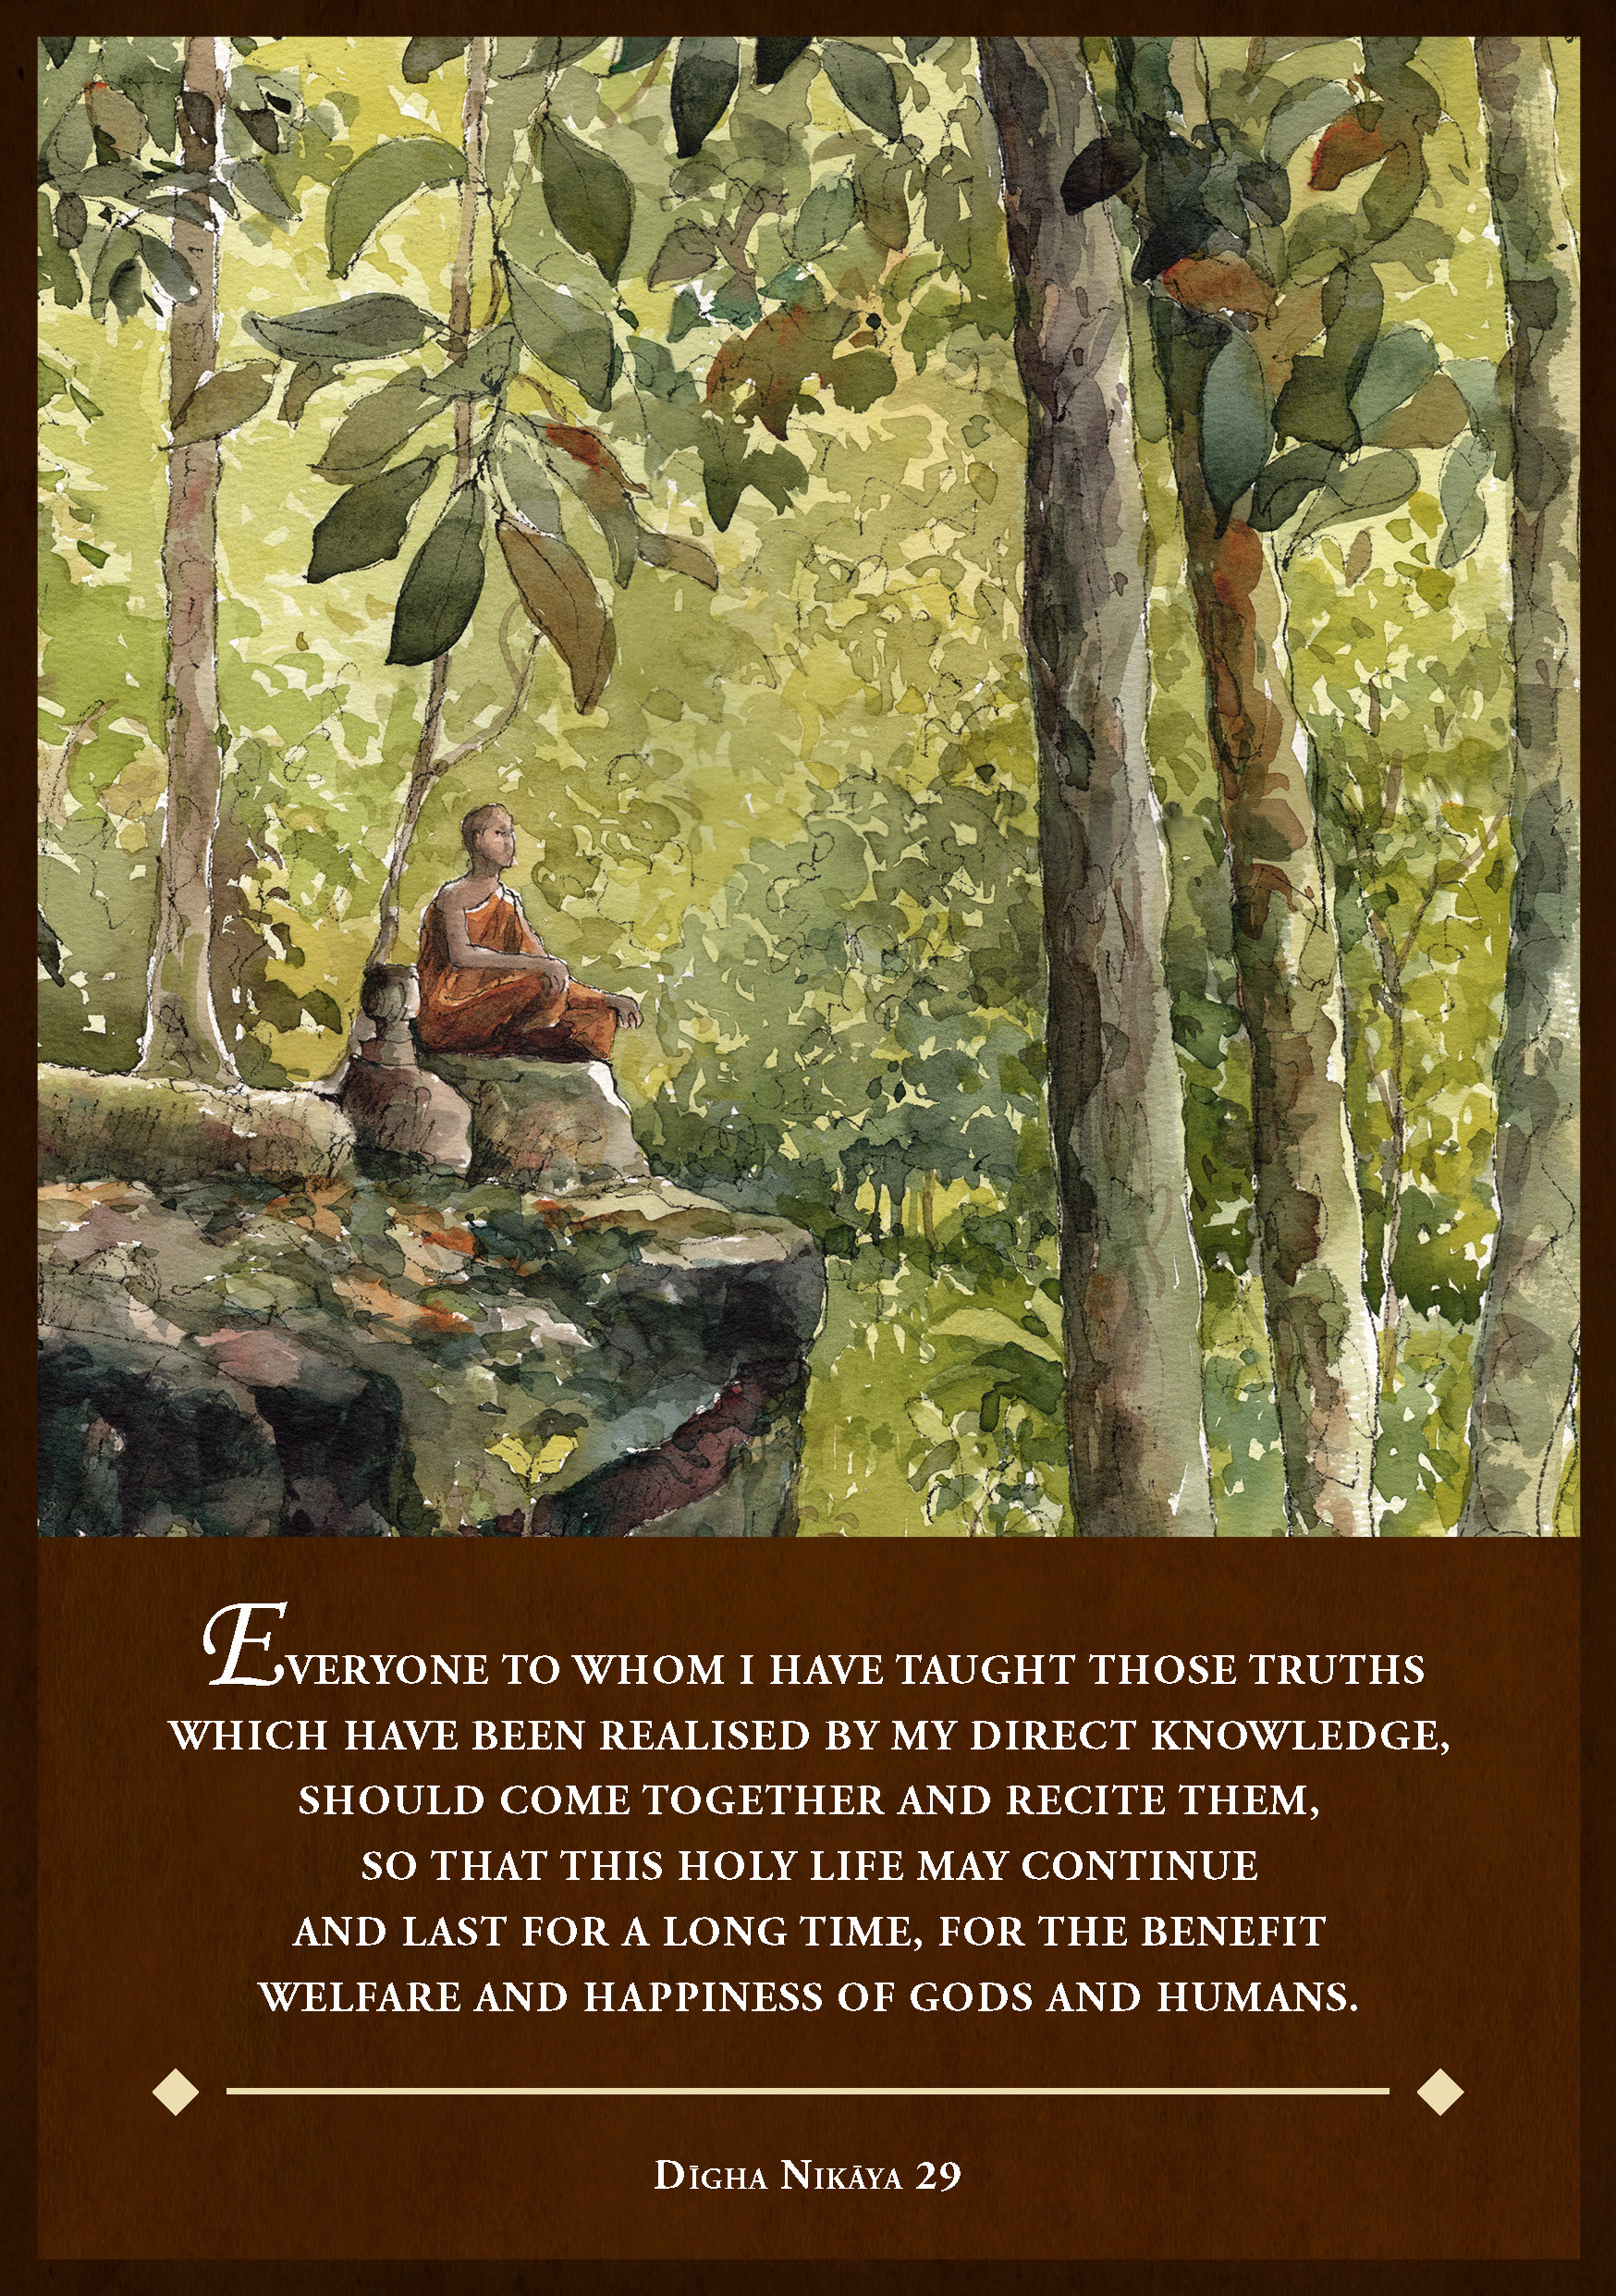
\includegraphics[height=\paperheight]{./assets/images/A5/back_cover_compressed_A5.jpg}}
\fi

\ifninebythirteenversion
  \photoFullBleed{./assets/images/9x13/back_cover_9x13.png}
\fi

\ifbfiveversion
  \photoFullBleed{./assets/images/B5/back_cover_B5.png}
\fi

\end{document}
'
\ifdefined\isdigitalversion
  \newcommand{\digitaloption}{digitalVersion}
\else
  \newcommand{\digitaloption}{}
\fi
\typeout{Set \protect\digitaloption{} to \digitaloption}

% todo ask bergen to make showtims a togglable condition for b5 and 9x13 only

\documentclass[
  final,
  babelLanguage=british,
  showtrims,
  \papersizeoption,
  \digitaloption,
]{anecdote}

% Define graphics path for images
\graphicspath{
  {./assets/images/A5}
  {./assets/images/9x13}
  {./assets/images/B5}
  {./assets/images/graphics}
}

% Loads formatting for selected ddocument class
\ifninebythirteenversion \usepackage{9x13} \fi
\ifafiveversion \usepackage{A5} \fi
\ifbfiveversion \usepackage{B5} \fi

% Set metadata for the document
\title{SBS Pāli-English Recitations}
\subtitle{Monk Training Centre}
\author{SBS Monk Training Centre}
\publisher{Sāsanārakkha Buddhist Sanctuary}
\date{2021-10-30}
\editionInfo{\textit{First Edition}, 2025} % And last edition. Don't call Pāladhammika.
\newcommand{\MyISBN}{} % default empty

\ifbfiveversion
  \renewcommand{\MyISBN}{978-629-97831-1-4}
\fi
\ifninebythirteenversion
  \renewcommand{\MyISBN}{978-629-97831-2-1}
\fi

\ISBN{\MyISBN}

% Set metadata for PDF properties
\hypersetup{
  pdftitle={\thetitle},
  pdfauthor={\theauthor},
  pdfcopyright={Copyright (C) 2025, \thePublisher},
  pdfsubject={},
  pdfkeywords={},
  pdflicenseurl={https://creativecommons.org/licenses/by-nc-nd/4.0/},
  pdfcontacturl={},
  pdflang={en},
}

% Load further packages
\RequirePackage[yyyymmdd,hhmmss]{datetime} % Adds the time to version creation

\makepagenote
\continuousnotenums % Ensure continuous endnote numbering

% Define hyphenation exceptions and corrections
\hyphenation{London re-lin-quishes de-ter-mines}

\ifdigitalversion
  \openany
\fi

% Begin document
\begin{document}

% Front matter
\frontmatter

% Digital version cover
\ifdigitalversion
	\digitalCover{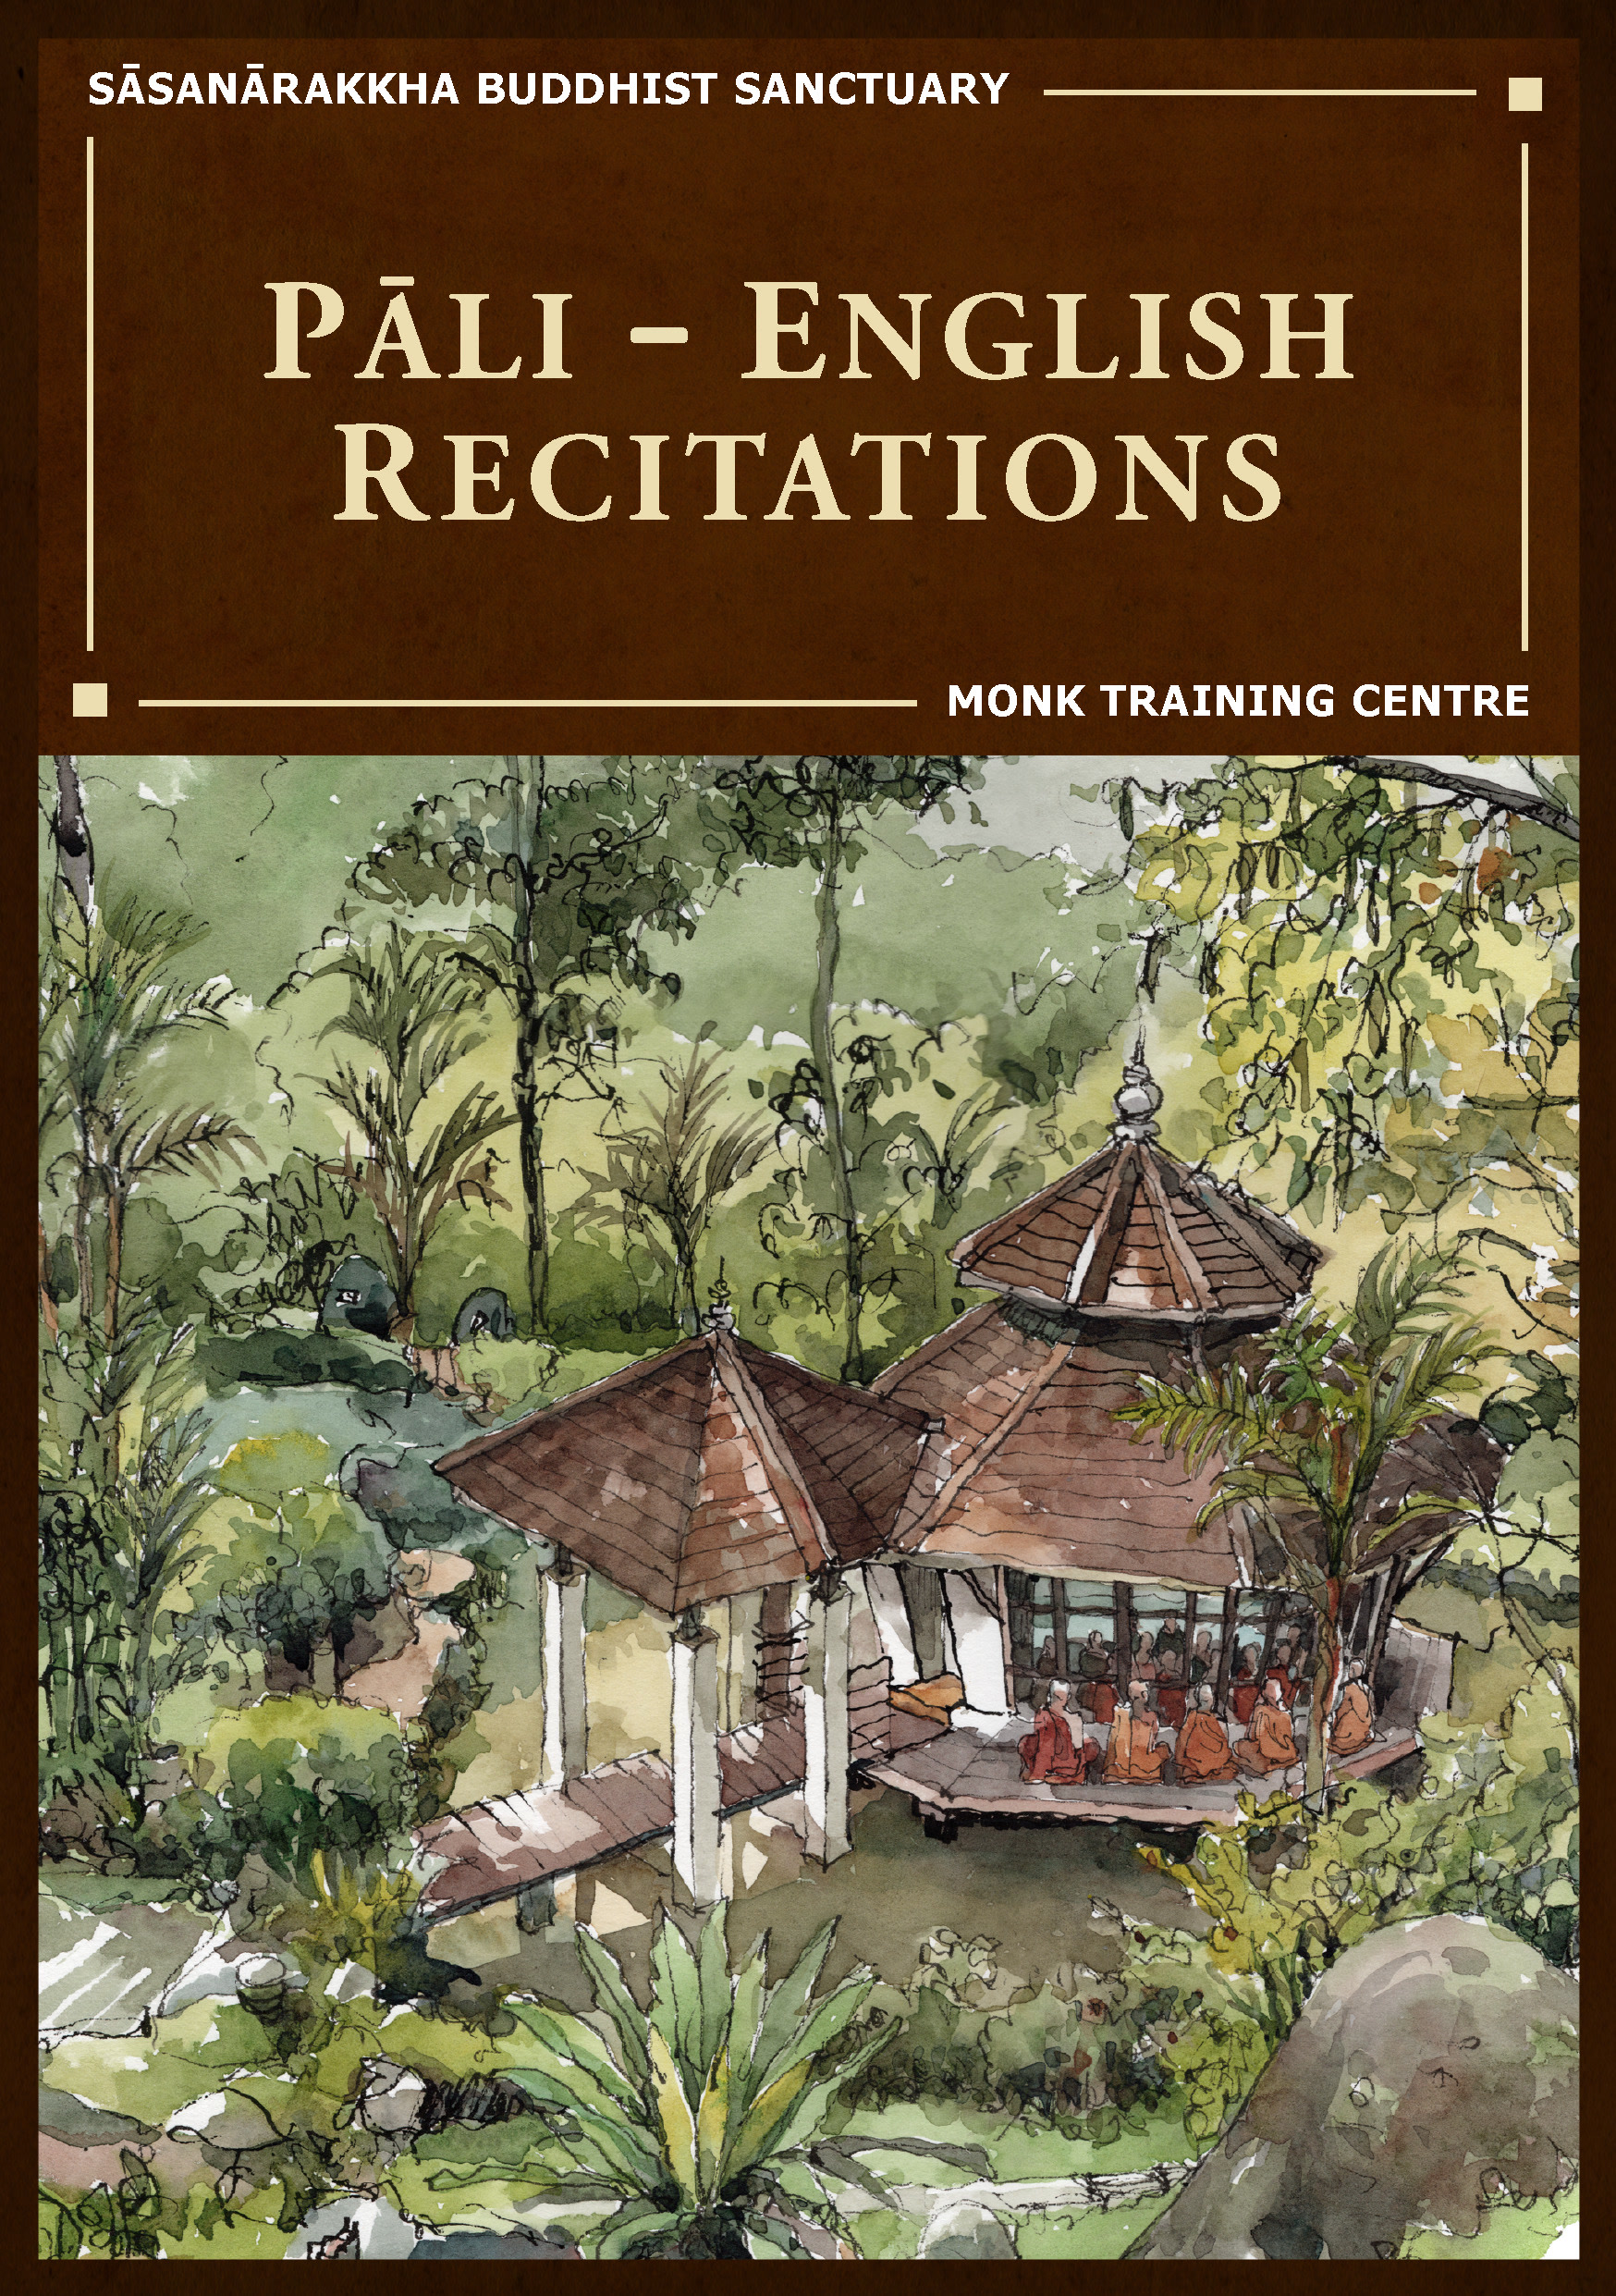
\includegraphics[height=\paperheight]{./assets/images/A5/front_cover_compressed_A5.jpg}}
\fi

\ifninebythirteenversion
  \photoFullBleed{./assets/images/9x13/front_cover_9x13.png}
  \photoFullBleed{robe_divider_left_9x13.png}
  \photoFullBleed{robe_divider_right_9x13.png}
\fi

\ifbfiveversion
  \photoFullBleed{./assets/images/B5/front_cover_B5.png}
  \photoFullBleed{robe_divider_left_B5.png}
  \photoFullBleed{robe_divider_right_B5.png}
\fi

% Title page, copyright, acknowledgments
\pagestyle{empty}

\cleartorecto
\thispagestyle{empty}

\vspace*{3em}

{\centering

  \settowidth{\titleLength}{%
    {\Large\chapterTitleFont\textsc{\MakeUppercase{{Pāli-English Recitations}}}}%
  }

  % 'SBS' on title page
  \ifafive {\Huge\fontsize{64}{16}\sbsFont SBS}\\[1.0\baselineskip] \fi
  \ifninebythirteen {\Huge\fontsize{42.5}{11}\sbsFont SBS}\\[1.0\baselineskip] \fi
  \ifbfive {\Huge\fontsize{80}{16}\sbsFont SBS}\\[1.0\baselineskip] \fi

  % 'Monk Training Centre'
  \ifafive \setlength{\xheight}{\heightof{X}}
    {\Huge\chapterTitleFont\textsc{{\thesubtitle\linebreak}}}\\[0.2\baselineskip] \fi
  \ifninebythirteen {\fontsize{16}{14}\chapterTitleFont\textsc{{\thesubtitle\linebreak}}}\\[0.2\baselineskip] \fi
  \ifbfive \setlength{\xheight}{\heightof{X}}
    {\fontsize{30}{14}\chapterTitleFont\textsc{{\thesubtitle\linebreak}}}\\[0.2\baselineskip] \fi

  % Ornament
  \ifafive \raisebox{0.5\xheight}{\pgfornament[color=sbs-brown,width=7cm,scale=1,ydelta=0pt,symmetry=c]{84}}\\[1.4\baselineskip] \fi
  \ifninebythirteen \raisebox{0.5\xheight}{\pgfornament[color=sbs-brown,width=4.5cm,scale=1,ydelta=0pt,symmetry=c]{84}}\\[1.4\baselineskip] \fi
  \ifbfive \raisebox{0.5\xheight}{\pgfornament[color=sbs-brown,width=8.5cm,scale=1,ydelta=0pt,symmetry=c]{84}}\\[1.4\baselineskip] \fi


  % 'Pali-English Recitations'
  \ifafive {\Large\scshape Pāli-English Recitations}\\[2.5\baselineskip] \fi
  \ifninebythirteen {\fontsize{10}{12}\scshape Pāli-English Recitations}\\[2.5\baselineskip] \fi
  \ifbfive {\fontsize{18.5}{12}\scshape Pāli-English Recitations}\\[2.5\baselineskip] \fi

  % Dhamma quote
  {\quote ``In whatever way a bhikkhu recites the Dhamma in detail as he has heard it and learned it, in just that way, in relation to that Dhamma, he experiences inspiration in the meaning and inspiration in the Dhamma. As he does so, joy arises in him. When he is joyful, rapture arises. For one with a rapturous mind, the body becomes tranquil. One tranquil in body feels pleasure. For one feeling pleasure, the mind becomes concentrated.''\\}
  \ifafive \smallskip AN 5.26\\[1.4\baselineskip]\fi
  \ifninebythirteen \smallskip \fontsize{8}{14}\selectfont AN 5.26\\[1.4\baselineskip]\fi
  %% \ifbfive \smallskip \fontsize{8.5}{14}\selectfont AN 5.26\\[1.4\baselineskip]\fi
  \ifbfive \smallskip AN 5.26\\[1.4\baselineskip]\fi
}



\cleartoverso
\thispagestyle{empty}

{%

  \ifafive \fontsize{10}{16}\selectfont \fi
  \ifninebythirteen \fontsize{7.5}{11}\selectfont \fi
  \ifbfive \fontsize{12}{20}\selectfont \fi
  \centering
  \setlength{\parindent}{0pt}%

  \ifafive \vspace{0.5cm} \fi
  \ifninebythirteen \vspace{0.4cm} \fi
  \ifbfive \vspace{0.5cm} \fi

  \copyright\ \thePublisher, 2025\\
  c/o 160, Lorong 3, Jalan Merdeka, 34000 Taiping, Perak, Malaysia\\
  \ifdigital
    \else
  ISBN \theISBN
  \fi

  \ifafive \vspace{0.5cm} \fi
  \ifninebythirteen \vspace{0.3cm} \fi
  \ifbfive \vspace{0.5cm} \fi

  This book is for free distribution only;\\
  it may not be sold.

  \ifafive \vspace{0.5cm} \fi
  \ifninebythirteen \vspace{0.3cm} \fi
  \ifbfive \vspace{0.5cm} \fi

  Download this book as a PDF, EPUB, MOBI, AZW3\\
  at the following address:\\
  \href{https://sasanarakkha.org/recitations}{https://sasanarakkha.org/recitations}

Accompanying audio recordings can be found at:
\href{https://www.youtube.com/SasanarakkhaBuddhistSanctuary}{https://www.youtube.com/SasanarakkhaBuddhistSanctuary}

  \ifafive \vspace{0.5cm} \fi
  \ifninebythirteen \vspace{0.3cm} \fi
  \ifbfive \vspace{0.5cm} \fi

  Project Manager: Ā. Ariyadhammika\\
  Editor: Ā. Pāladhammika\\
  Typesetting: Aj. Gambhiro, Ā. Pāladhammika\\
  Translators: Ā. Aggacitta, Ā. Bodhi, Aj. Kevalī, Ā. Sujāto, M. Walshe\\
  Endnotes: Ā. Ariyadhammika\\
  Watercolor Paintings: Lim Jee Yuan

  \ifafive \vspace{0.5cm} \fi
  \ifninebythirteen \vspace{0.3cm} \fi
  \ifbfive \vspace{0.5cm} \fi

  This work is licensed under a Creative Commons\\
  Attribution-NonCommercial-NoDerivatives 4.0 International~License.

  % Produced with the \LaTeX\ typesetting system,\\
  % set in Libertinus Serif.

  \ifafive  \vspace{0.5cm} \fi
  \ifninebythirteen \vspace{0.3cm} \fi
  \ifbfive \vspace{0.5cm} \fi

  \ifdigital
    This version was created on:\\
    \today \space at \currenttime\\
  \fi

  \ifafive \vspace{0.5cm} \fi
  \ifninebythirteen \vspace{0.15cm} \fi
  \ifbfive \vspace{0.5cm} \fi

  \theEditionInfo

}

\ifdigital

\else

\clearpage

\fi



\cleartorecto
\thispagestyle{empty}

{

  \setlength{\parskip}{10pt}

  \ifafive {\centering\fontsize{16}{25}\selectfont \textsc{We Wish To Gratefully Acknowledge} \par} \fi
  \ifninebythirteen {\centering\fontsize{10}{18}\selectfont \textsc{We Wish To Gratefully Acknowledge} \par} \fi
  \ifbfive {\centering\fontsize{18.5}{25}\selectfont \textsc{We Wish To Gratefully Acknowledge} \par} \fi


  The Saṅghas of Wat Pah Nanachat (WPN), Amaravati, and Abhayagiri for allowing the use of material from their respective chanting books, the late Ven. Dr. Saddhātissa and Mr. Maurice Walshe for their English translations, as well as Ven. Bhikkhu Bodhi for granting permission to use and slightly adapt his translations. Various Saṅgha members of SBS Monk Training Centre, who contributed in the compilation of an interesting selection of chants, as well as for providing countless suggestions to help improve the English translations.

  \linkdest{endnote1-body}
  Additional information on translations, as well as deviations\makeatletter\hyperlink{endnote1-appendix}\Hy@raisedlink{{\pagenote{%
        \hypertarget{endnote1-appendix}{\hyperlink{endnote1-body}{Due to the balanced and inspiring selection of chants, as well as for the sake of compatibility, WPN’s \textit{Buddhist Chanting} (2014) has served as the basis for this book. Over time, suggestions for the inclusion of additional chants, as well as occasional improvements of existing translations were incorporated. Such changes were meticulously marked down in the endnotes of the digital versions of this chanting book, so that someone familiar with the present book can straight away find the relevant differences, which can be useful when visiting a branch monastery of the Ajahn Chah lineage, in order to know in which places to revert to the original version.}}}}}\makeatother\thickspace
  from WPN's \textit{Buddhist Chanting} (2014), have been annotated by Ven. Ariyadhammika in the endnotes.


  \ifninebythirteen \smallskip \else \medskip \fi

  {\centering

    To Āyasmā Aggacitta, the founding father of\\
    Sāsanārakkha Buddhist Sanctuary.

    % \ifninebythirteen \smallskip \else \medskip \fi

    \begin{center}
      \ifafive 
\includegraphics[height=54mm]{sbs_logo_tuck_loon_brown.jpg} \fi
      \ifninebythirteen \clearpage \vspace*{\fill}
 
\includegraphics[height=80mm]{sbs_logo_tuck_loon_brown.jpg} \vspace*{\fill} \fi
      \ifbfive \vspace{1cm} 
\includegraphics[height=70mm]{sbs_logo_tuck_loon_brown.jpg}\fi
    \end{center}
  }
}



% Table of contents, schedule, purpose and benefits, abbreviations
\cleartorecto
\pagestyle{toponerow-frontmatter}
\chapterstyle{adrasteia-toc}

\pdfbookmark[section]{\contentsname}{toc}
\tableofcontents*


\chapter{Recitation Schedule}
\label{schedule}

{\centering

  {\pdfbookmark[2]{Set 1}{set1}\libertinusFont\selectfont\textbf{\textsc{\ifafive\fontsize{18}{12}\fi\ifninebythirteen\fontsize{13}{8.5}\fi\ifbfive\fontsize{22}{18}\fi\selectfont\textls*{Set 1}}}}\\
  \textsc{\ifafive\fontsize{14.4}{28}\fi\ifninebythirteen\fontsize{8.7}{17}\fi\ifbfive\fontsize{16}{33.5}\fi\selectfont
    \hyperref[buddhas-first-exclamation]{The Buddha's First Exclamation} \ifdigital\else\pageref{buddhas-first-exclamation}\fi\\
    \hyperref[wheel-of-dhamma-abridged]{Turning the Wheel of Dhamma} \ifdigital\else\pageref{wheel-of-dhamma-abridged}\fi\\
    \hyperref[true-false-refuges]{Going to True and False Refuges} \ifdigital\else\pageref{true-false-refuges}\fi\\
    \hyperref[four-great-references]{The Four Great References} \ifdigital\else\pageref{four-great-references}\fi\\
    \hyperref[patimokkha-exhortation]{The Pāṭimokkha Exhortation} \ifdigital\else\pageref{patimokkha-exhortation}\fi\\
    \hyperref[buddhas-final-instruction]{The Buddha's Final Instruction} \ifdigital\else\pageref{buddhas-final-instruction}\fi\\
    \hyperref[uddissanadhitthana]{Sharing and Aspirations (Pāli)} \ifdigital\else\pageref{uddissanadhitthana}\fi\\
    \hyperref[closing-homage]{Closing Homage (Pāli-English)} \ifdigital\else\pageref{closing-homage}\fi\\
  }

  \ifafive\vspace{1.0cm}\fi
  \ifninebythirteen\vspace{0.8cm}\fi
  \ifbfive\vspace{1.0cm}\fi

  {\pdfbookmark[2]{Set 2}{set2}\libertinusFont\selectfont\textbf{\textsc{\ifafive\fontsize{18}{12}\fi\ifninebythirteen\fontsize{13}{8.5}\fi\ifbfive\fontsize{22}{18}\fi\selectfont\textls*{Set 2}}}}\\
  \textsc{\ifafive\fontsize{14.4}{28}\fi\ifninebythirteen\fontsize{8.7}{17}\fi\ifbfive\fontsize{16}{33.5}\fi\selectfont
    \hyperref[characteristic-of-not-self]{The Discourse on the Characteristic of Not-Self} \ifdigital\else\pageref{characteristic-of-not-self}\fi\\
    \hyperref[exposition-on-burning]{The Discourse on the Exposition on Burning} \ifdigital\else\pageref{exposition-on-burning}\fi\\
    \hyperref[gradual-training]{The Gradual Training} \ifdigital\else\pageref{gradual-training}\fi\\
    \hyperref[sharing-aspirations]{Sharing and Aspirations (English)} \ifdigital\else\pageref{sharing-aspirations}\fi\\
    \hyperref[closing-homage]{Closing Homage (English)} \ifdigital\else\pageref{closing-homage}\fi\\
  }

  \clearpage

  {\pdfbookmark[2]{Set 3}{set3}\libertinusFont\selectfont\textbf{\textsc{\ifafive\fontsize{18}{12}\fi\ifninebythirteen\fontsize{13}{8.5}\fi\ifbfive\fontsize{22}{18}\fi\selectfont\textls*{Set 3}}}}\\

\textsc{\ifafive\fontsize{14.4}{28}\fi\ifninebythirteen\fontsize{8.7}{17}\fi\ifbfive\fontsize{16}{33.5}\fi\selectfont
    \hyperref[noble-eightfold-path]{The Noble Eightfold Path} \ifdigital\else\pageref{noble-eightfold-path}\fi\\
    \hyperref[repulsiveness-of-food]{The Repulsiveness of Food} \ifdigital\else\pageref{repulsiveness-of-food}\fi\\
    \hyperref[requisites-for-awakening]{Requisites for Awakening} \ifdigital\else\pageref{requisites-for-awakening}\fi\\
    \hyperref[principles-of-non-decline]{Principles of Non-Decline} \ifdigital\else\pageref{principles-of-non-decline}\fi\\
    \hyperref[protection]{On Protection} \ifdigital\else\pageref{protection}\fi\\
    \hyperref[sharing-all-merits]{Sharing of All Merits} \ifdigital\else\pageref{sharing-all-merits}\fi\\
    \hyperref[closing-homage]{Closing Homage (Pāli-English)} \ifdigital\else\pageref{closing-homage}\fi\\
  }

  \ifafive\vspace{1.0cm}\fi
  \ifninebythirteen\vspace{0.8cm}\fi
  \ifbfive\vspace{1.0cm}\fi

  {\pdfbookmark[2]{Set 4}{set4}\libertinusFont\selectfont\textbf{\textsc{\ifafive\fontsize{18}{12}\fi\ifninebythirteen\fontsize{13}{8.5}\fi\ifbfive\fontsize{22}{18}\fi\selectfont\textls*{Set 4}}}}\\

\textsc{\ifafive\fontsize{14.4}{28}\fi\ifninebythirteen\fontsize{8.7}{17}\fi\ifbfive\fontsize{16}{33.5}\fi\selectfont
    \hyperref[dedication-of-offerings]{Homage to the Triple Gem} \ifdigital\else\pageref{dedication-of-offerings}\fi\\
    \hyperref[universal-well-being]{Universal Well-Being} \ifdigital\else\pageref{universal-well-being}\fi\\
    \hyperref[seven-factors-of-awakening]{The Seven Factors of Awakening} \ifdigital\else\pageref{seven-factors-of-awakening}\fi\\
    \hyperref[words-on-loving-kindness]{The Buddha's Words on Loving-Kindness} \ifdigital\else\pageref{words-on-loving-kindness}\fi\\
    \hyperref[sharing-merits-departed]{Sharing of Merits with \ifninebythirteen\\[-0.6em]\fi the Departed (Pāli-English)} \ifdigital\else\pageref{sharing-merits-departed}\fi\\
    \hyperref[sharing-merits-devas]{Sharing of Merits with the Devas (Pāli-English)} \ifdigital\else\pageref{sharing-merits-devas}\fi\\
    \hyperref[closing-homage]{Closing Homage (Pāli-English)} \ifdigital\else\pageref{closing-homage}\fi\\
  }

  \clearpage

  {\pdfbookmark[2]{Set 5}{set5}\libertinusFont\selectfont\textbf{\textsc{\ifafive\fontsize{18}{12}\fi\ifninebythirteen\fontsize{13}{8.5}\fi\ifbfive\fontsize{22}{18}\fi\selectfont\textls*{Set 5}}}}\\
  \textsc{\ifafive\fontsize{14.4}{28}\fi\ifninebythirteen\fontsize{8.7}{17}\fi\ifbfive\fontsize{16}{33.5}\fi\selectfont
    \hyperref[mindfulness-of-breathing]{Mindfulness of Breathing} \ifdigital\else\pageref{mindfulness-of-breathing}\fi\\
    \hyperref[discourse-on-blessings]{The Discourse on Blessings} \ifdigital\else\pageref{discourse-on-blessings}\fi\\
    \hyperref[three-characteristics]{The Three Characteristics} \ifdigital\else\pageref{three-characteristics}\fi\\
    \hyperref[four-requisites]{The Four Requisites} \ifdigital\else\pageref{four-requisites}\fi\\
    \hyperref[five-reflections]{Five Subjects for Frequent Reflection} \ifdigital\else\pageref{five-reflections}\fi\\
    \hyperref[32-parts]{The Thirty-Two Body Parts} \ifdigital\else\pageref{32-parts}\fi\\
    \hyperref[principles-of-cordiality]{Principles of Cordiality} \ifdigital\else\pageref{principles-of-cordiality}\fi\\
    \hyperref[highest-honour-aspirations]{The Highest Honour and Aspirations} \ifdigital\else\pageref{highest-honour-aspirations}\fi\\
    \hyperref[closing-homage]{Closing Homage (Pāli-English)} \ifdigital\else\pageref{closing-homage}\fi\\
  }

  \ifafive\vspace{1.0cm}\fi
  \ifninebythirteen\vspace{0.8cm}\fi
  \ifbfive\vspace{1.0cm}\fi

  {\pdfbookmark[2]{Set 6}{set6}\libertinusFont\selectfont\textbf{\textsc{\ifafive\fontsize{18}{12}\fi\ifninebythirteen\fontsize{13}{8.5}\fi\ifbfive\fontsize{22}{18}\fi\selectfont\textls*{Set 6}}}}\\
  \textsc{\ifafive\fontsize{14.4}{28}\fi\ifninebythirteen\fontsize{8.7}{17}\fi\ifbfive\fontsize{16}{33.5}\fi\selectfont
    \hyperref[anatta-lakkhana]{Anatta-lakkhaṇa Sutta} \ifdigital\else\pageref{anatta-lakkhana}\fi\\
    \hyperref[striving-according-to-dhamma]{Striving According to the Dhamma} \ifdigital\else\pageref{striving-according-to-dhamma}\fi\\
    \hyperref[divine-abidings]{The Divine Abidings} \ifdigital\else\pageref{divine-abidings}\fi\\
    \hyperref[ten-reflections]{Ten Subjects for Frequent Reflection\\ \ifafive\vspace{-0.4cm}\fi \ifbfive\vspace{-0.4cm}\fi \ifninebythirteen\vspace{-0.2cm}\fi by One Gone Forth} \ifdigital\else\pageref{ten-reflections}\fi\\
    \hyperref[sharing-aspirations]{Sharing and Aspirations (English)} \ifdigital\else\pageref{sharing-aspirations}\fi\\
    \hyperref[closing-homage]{Closing Homage (Pāli-English)} \ifdigital\else\pageref{closing-homage}\fi\\
  }

  \clearpage

  {\pdfbookmark[2]{Set 7}{set7}\libertinusFont\selectfont\textbf{\textsc{\ifafive\fontsize{18}{12}\fi\ifninebythirteen\fontsize{13}{8.5}\fi\ifbfive\fontsize{22}{18}\fi\selectfont\textls*{Set 7}}}}\\
  \textsc{\ifafive\fontsize{14.4}{28}\fi\ifninebythirteen\fontsize{8.7}{17}\fi\ifbfive\fontsize{16}{33.5}\fi\selectfont
    \hyperref[dependent-origination]{Dependent Origination} \ifdigital\else\pageref{dependent-origination}\fi\\
    \hyperref[dhamma-in-brief]{The Dhamma in Brief} \ifdigital\else\pageref{dhamma-in-brief}\fi\\
    \hyperref[uddissanadhitthana]{Sharing and Aspirations (Pāli)} \ifdigital\else\pageref{uddissanadhitthana}\fi\\
    \hyperref[closing-homage]{Closing Homage (Pāli-English)} \ifdigital\else\pageref{closing-homage}\fi\\
  }

  \ifafive\vspace{1.0cm}\fi
  \ifninebythirteen\vspace{0.8cm}\fi
  \ifbfive\vspace{1.0cm}\fi

  {\pdfbookmark[2]{Set 8}{set8}\libertinusFont\selectfont\textbf{\textsc{\ifafive\fontsize{18}{12}\fi\ifninebythirteen\fontsize{13}{8.5}\fi\ifbfive\fontsize{22}{18}\fi\selectfont\textls*{Set 8}}}}\\
  \textsc{\ifafive\fontsize{14.4}{28}\fi\ifninebythirteen\fontsize{8.7}{17}\fi\ifbfive\fontsize{16}{33.5}\fi\selectfont
    \hyperref[aditta-pariyaya]{Āditta-Pariyāya Sutta} \ifdigital\else\pageref{aditta-pariyaya}\fi\\
    \hyperref[burdens]{The Burdens} \ifdigital\else\pageref{burdens}\fi\\
    \hyperref[respect-for-the-dhamma]{Respect for the Dhamma} \ifdigital\else\pageref{respect-for-the-dhamma}\fi\\
    \hyperref[single-excellent-night]{A Single Excellent Night} \ifdigital\else\pageref{single-excellent-night}\fi\\
    \hyperref[ratthapala]{From the Elder Raṭṭhapāla}  \ifdigital\else\pageref{ratthapala}\fi\\
    \hyperref[parapariya]{From the Elder Pārāpariya} \ifdigital\else\pageref{parapariya}\fi\\
    \hyperref[misc-verses]{Miscellaneous Verses} \ifdigital\else\pageref{misc-verses}\fi\\
    \hyperref[highest-honour-aspirations]{The Highest Honour and Aspirations} \ifdigital\else\pageref{highest-honour-aspirations}\fi\\
    \hyperref[closing-homage]{Closing Homage (Pāli-English)} \ifdigital\else\pageref{closing-homage}\fi\\
  }

  \clearpage

  {\pdfbookmark[2]{Set 9}{set9}\libertinusFont\selectfont\textbf{\textsc{\ifafive\fontsize{18}{12}\fi\ifninebythirteen\fontsize{13}{8.5}\fi\ifbfive\fontsize{22}{18}\fi\selectfont\textls*{Set 9}}}}\\
  \textsc{\ifafive\fontsize{14.4}{28}\fi\ifninebythirteen\fontsize{8.7}{17}\fi\ifbfive\fontsize{16}{33.5}\fi\selectfont
    \hyperref[invitation-to-the-devas]{Protective Recitations (Pāli)} \ifdigital\else\pageref{invitation-to-the-devas}\fi\\
    \hyperref[sharing-merits-departed]{Sharing of Merits with the Departed (Pāli)} \ifdigital\else\pageref{sharing-merits-departed}\fi\\
    \hyperref[sharing-merits-devas]{Sharing of Merits with the Devas (Pāli)} \ifdigital\else\pageref{sharing-merits-devas}\fi\\
    \hyperref[closing-homage]{Closing Homage (Pāli)} \ifdigital\else\pageref{closing-homage}\fi\\
  }

  \ifafive\vspace{1.0cm}\fi
  \ifninebythirteen\vspace{0.8cm}\fi
  \ifbfive\vspace{1.0cm}\fi

  {\pdfbookmark[2]{Set 10}{set10}\libertinusFont\selectfont\textbf{\textsc{\ifafive\fontsize{18}{12}\fi\ifninebythirteen\fontsize{13}{8.5}\fi\ifbfive\fontsize{22}{18}\fi\selectfont\textls*{Set 10}}}}\\
\textsc{\ifafive\fontsize{14.4}{28}\fi\ifninebythirteen\fontsize{8.7}{17}\fi\ifbfive\fontsize{16}{33.5}\fi\selectfont
    \hyperref[passage-on-preliminary-paying-of-homage-funeral]{Funeral Recitations (Pāli)} \ifdigital\else\pageref{passage-on-preliminary-paying-of-homage-funeral}\fi\\
    \hyperref[recollection-of-impermanence]{Recollection of Impermanence} \ifdigital\else\pageref{recollection-of-impermanence}\fi\\
    \hyperref[just-as-rivers]{Thanksgiving Recitations} \ifdigital\else\pageref{just-as-rivers}\fi\\
    \hyperref[sharing-all-merits]{Sharing of All Merits} \ifdigital\else\pageref{sharing-all-merits}\fi\\
    \hyperref[closing-homage]{Closing Homage (Pāli-English)} \ifdigital\else\pageref{closing-homage}\fi\\
  }}


\input{./tex/purpose-and-benefits.tex}

\chapter{Abbreviations}
\label{abbreviations}

\ifafive
\begin{tabular}{@{}ll@{}}
  \anglebracketleft\ \hspace{-0.5mm}... \hspace{-0.85mm}\anglebracketright\ & \hspace{1.30mm}Only recited by the leader \\
  \hspace{0.1cm} \abbrbreathmark\ & \hspace{1.45mm}Breathing pause \\
\end{tabular}
\fi

\ifninebythirteen
\begin{tabular}{@{}ll@{}}
  \anglebracketleft\ \hspace{-0.5mm}... \hspace{-0.70mm}\anglebracketright\ & \hspace{1.10mm}Only recited by the leader \\
  \hspace{0.1cm} \abbrbreathmark\ & \hspace{1.20mm}Breathing pause \\
\end{tabular}
\fi

\ifbfive
\begin{tabular}{@{}ll@{}}
  \anglebracketleft\ \hspace{-0.5mm}... \hspace{-0.85mm}\anglebracketright\ & \hspace{2.70mm}Only recited by the leader \\
  \hspace{0.2cm} \abbrbreathmark\ & \hspace{2.90mm}Breathing pause \\
\end{tabular}
\fi

\ifninebythirteen

\vspace{-0.6em}
\begin{tabular}{@{}llll@{}}
  DN    & Dīgha Nikāya                                        \\
  MN    & Majjhima Nikāya                                     \\
  SN    & Saṁyutta Nikāya                                     \\
  AN    & Aṅguttara Nikāya                                    \\
  Kp    & Khuddakapāṭha                                       \\
  Dhp   & Dhammapada                                          \\
  Ud    & Udāna                                               \\
  Snp   & Sutta Nipāta                                        \\
  Thag  & Theragāthā                                          \\
  Ja    & Jātaka                                              \\
  Pv    & Petavatthu                                          \\
  Vibh  & Abhidhamma Vibhaṅga                                 \\
  Dhs   & Dhammasaṅganī                                       \\
  A     & Aṭṭhakathā (Commentary)                             \\
  MJG   & Mahā-jaya-maṅgala-gāthā (Sri Lanka)                 \\
  Trad  & Traditional post-canonical verses                   \\
  WPN   & Wat Pah Nanachat                                    \\
\end{tabular}

\else

\begin{tabular}{@{}llll@{}}
  DN    & Dīgha Nikāya                                        \\
  MN    & Majjhima Nikāya                                     \\
  SN    & Saṁyutta Nikāya                                     \\
  AN    & Aṅguttara Nikāya                                    \\
  Kp    & Khuddakapāṭha                                       \\
  Dhp   & Dhammapada                                          \\
  Ud    & Udāna                                               \\
  Snp   & Sutta Nipāta                                        \\
  Thag  & Theragāthā                                          \\
  Ja    & Jātaka                                              \\
  Pv    & Petavatthu                                          \\
  Vibh  & Abhidhamma Vibhaṅga                                 \\
  Dhs   & Dhammasaṅganī                                       \\
\end{tabular}

\begin{tabular}{@{}llll@{}}
  A     & Aṭṭhakathā (Commentary)                             \\
  MJG   & Mahā-jaya-maṅgala-gāthā (Sri Lanka)                 \\
  Trad  & Traditional post-canonical verses                   \\
  WPN   & Wat Pah Nanachat
\end{tabular}

\medskip

\fi



\chapterstyle{adrasteia-frontmatter}

% Main matter
\mainmatter
\pagestyle{toponerow}

\cleartorecto

% Chapters
{\raggedright
	\input{./tex/recitations/homage.tex}
	\input{./tex/recitations/verses.tex}
	\input{./tex/recitations/teachings.tex}
	\input{./tex/recitations/reflections.tex}
	
\ifdigitalversion
  \chapterOpeningPage{cardinal_discourses_compressed_A5.jpg}
\else
  \chapterOpeningPage{cardinal_discourses_A5.jpg}
\fi

\ifninebythirteenversion
  \chapterOpeningPage{cardinal_discourses_9x13.png}
\fi

\ifbfiveversion
  \chapterOpeningPage{cardinal_discourses_B5.png}
\fi

\chapter{Cardinal Discourses}

\ifbfiveversion
  \photoFullBleed{assets/images/B5/brown_divider_B5.pdf}
\fi

\ifninebythirteenversion
  \photoFullBleed{assets/images/9x13/brown_divider_9x13.pdf}\fi

\input{./tex/recitations/cardinal-discourses/dhammacakkappavattana.tex}

\clearpage

\input{./tex/recitations/cardinal-discourses/dhammacakkappavattana-eng.tex}

\clearpage

\input{./tex/recitations/cardinal-discourses/anattalakkhana.tex}

\clearpage

\input{./tex/recitations/cardinal-discourses/anattalakkhana-eng.tex}

\clearpage

\input{./tex/recitations/cardinal-discourses/adittapariyaya.tex}

\clearpage

\input{./tex/recitations/cardinal-discourses/adittapariyaya-eng.tex}

\clearpage


	\input{./tex/recitations/thanksgiving-recitations.tex}
	\input{./tex/recitations/protective-recitations.tex}
	\input{./tex/recitations/funeral-recitations.tex}
	\input{./tex/recitations/sharing-of-merits.tex}
}

% Appendix
\appendix

\ifdigitalversion
  \chapterOpeningPage{appendix_compressed_A5.jpg}
\else
  \chapterOpeningPage{appendix_A5.jpg}
\fi

\ifninebythirteenversion
  \chapterOpeningPage{appendix_9x13.jpg}
\fi

\ifbfiveversion
  \chapterOpeningPage{appendix_B5.jpg}
\fi

\ifafiveversion\addtocontents{toc}{\protect\clearpage}\fi
\chapter{Appendix}

\ifbfiveversion
  \includepdf[pages=-]{assets/graphics/brown-texture_B5.pdf}
\fi

\ifninebythirteenversion
  \includepdf[pages=-]{assets/graphics/brown-texture_9x13.pdf}
\fi

\clearpage


\input{./tex/refuge-trainings.tex}
\input{./tex/phonetics-pronunciation.tex}
\input{./tex/guidelines.tex}

% Back matter
\backmatter
\printpagenotes % Print endnotes
\input{./tex/copyright-details.tex}

\ifbfiveversion
  \includepdf[pages=-,pagecommand={\thispagestyle{empty}}]{assets/images/graphics/donor-list.pdf}
  \photoFullBleed{robe_divider_left_B5.png}
  \photoFullBleed{robe_divider_right_B5.png}
\fi

\ifninebythirteenversion
  \photoFullBleed{robe_divider_left_9x13.png}
  \photoFullBleed{robe_divider_right_9x13.png}
\fi

\emptyUntilEven % Add blank page if necessary

\ifdigitalversion
  \clearpage
  \digitalCover{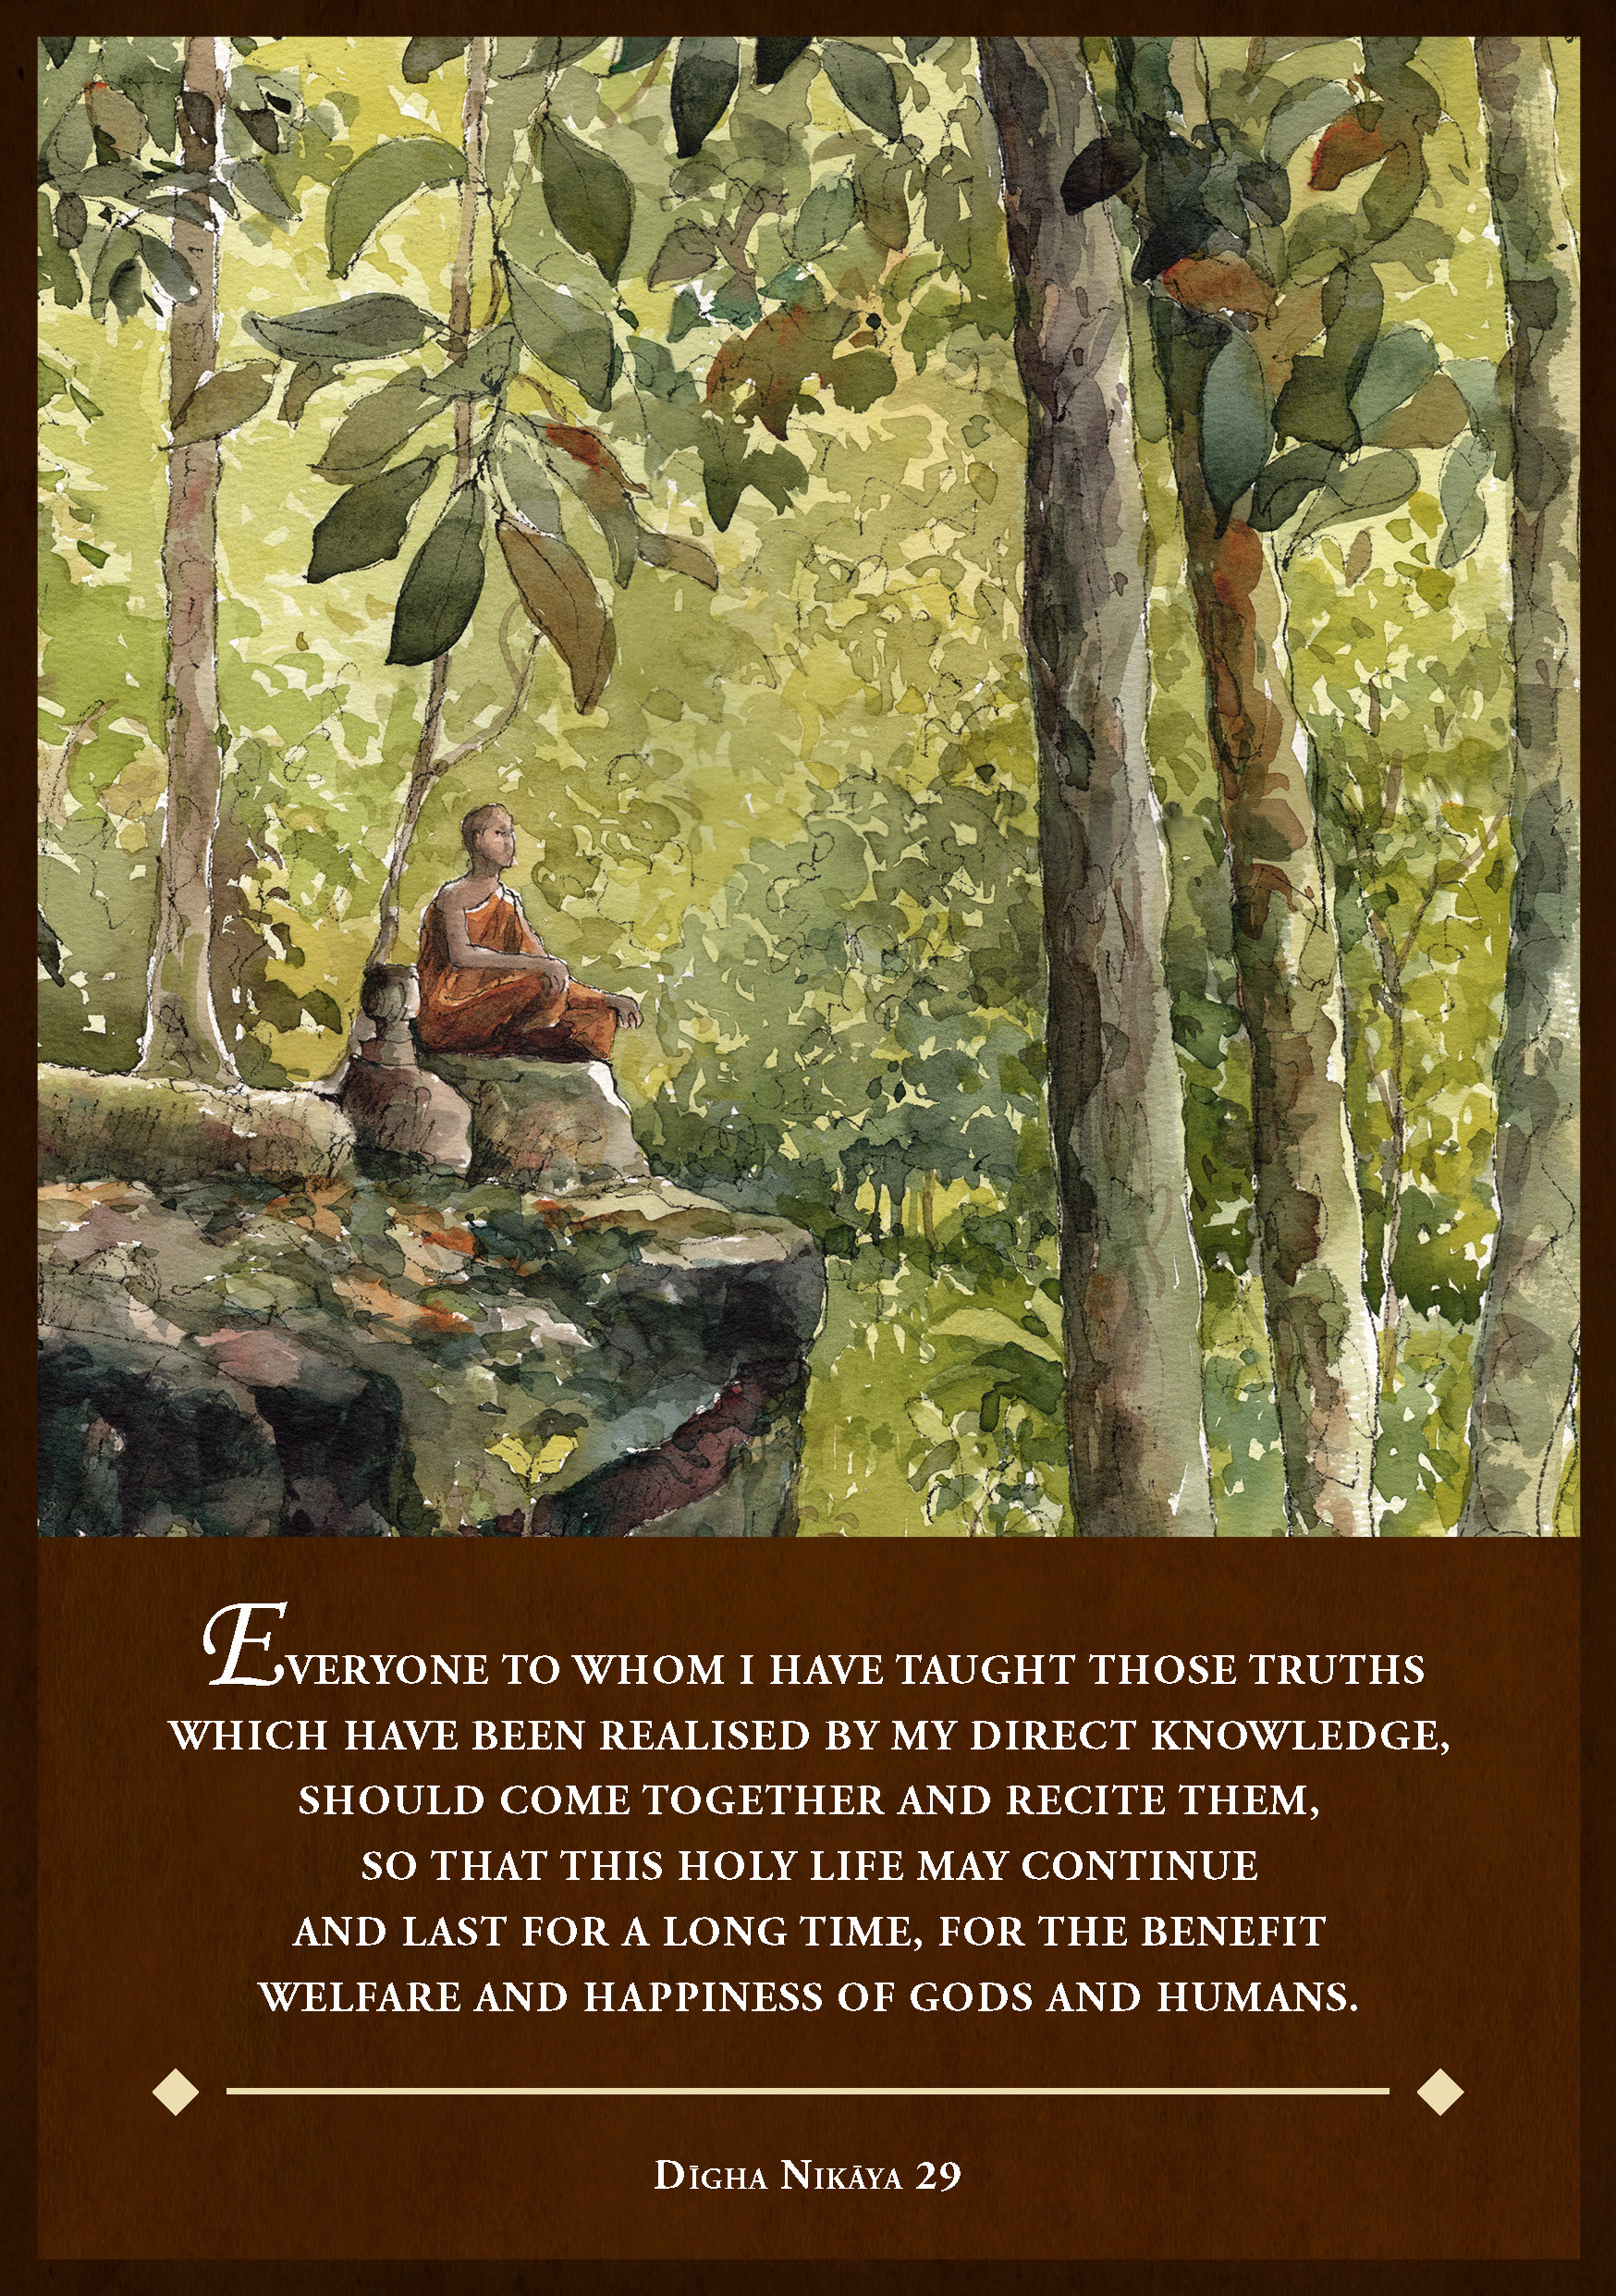
\includegraphics[height=\paperheight]{./assets/images/A5/back_cover_compressed_A5.jpg}}
\fi

\ifninebythirteenversion
  \photoFullBleed{./assets/images/9x13/back_cover_9x13.png}
\fi

\ifbfiveversion
  \photoFullBleed{./assets/images/B5/back_cover_B5.png}
\fi

\end{document}
'
% Possible VALUE:
%   - afiveVersion —  A5 formatted
%   - ninebythirteenVersion —  9x13cm custom formatted
%   - bfiveVersion —  B5 formatted
% \listfiles
\ifdefined\papersizeoption
\else
  \newcommand{\papersizeoption}{bfiveVersion}
\fi
\typeout{Set \protect\papersizeoption{} to \papersizeoption}

% Add hyperlinks and images, to be used with afiveVersion \papersizeoption
% Build command:
% '\newcommand{\papersizeoption}{afiveVersion}\newcommand{\isdigitalversion}{}% Set paper variant
% Build command '\newcommand{\papersizeoption}{VALUE}% Set paper variant
% Build command '\newcommand{\papersizeoption}{VALUE}% Set paper variant
% Build command '\newcommand{\papersizeoption}{VALUE}\input{main.tex}'
% Possible VALUE:
%   - afiveVersion —  A5 formatted
%   - ninebythirteenVersion —  9x13cm custom formatted
%   - bfiveVersion —  B5 formatted
% \listfiles
\ifdefined\papersizeoption
\else
  \newcommand{\papersizeoption}{bfiveVersion}
\fi
\typeout{Set \protect\papersizeoption{} to \papersizeoption}

% Add hyperlinks and images, to be used with afiveVersion \papersizeoption
% Build command:
% '\newcommand{\papersizeoption}{afiveVersion}\newcommand{\isdigitalversion}{}\input{main.tex}'
\ifdefined\isdigitalversion
  \newcommand{\digitaloption}{digitalVersion}
\else
  \newcommand{\digitaloption}{}
\fi
\typeout{Set \protect\digitaloption{} to \digitaloption}

% todo ask bergen to make showtims a togglable condition for b5 and 9x13 only

\documentclass[
  final,
  babelLanguage=british,
  showtrims,
  \papersizeoption,
  \digitaloption,
]{anecdote}

% Define graphics path for images
\graphicspath{
  {./assets/images/A5}
  {./assets/images/9x13}
  {./assets/images/B5}
  {./assets/images/graphics}
}

% Loads formatting for selected ddocument class
\ifninebythirteenversion \usepackage{9x13} \fi
\ifafiveversion \usepackage{A5} \fi
\ifbfiveversion \usepackage{B5} \fi

% Set metadata for the document
\title{SBS Pāli-English Recitations}
\subtitle{Monk Training Centre}
\author{SBS Monk Training Centre}
\publisher{Sāsanārakkha Buddhist Sanctuary}
\date{2021-10-30}
\editionInfo{\textit{First Edition}, 2025} % And last edition. Don't call Pāladhammika.
\newcommand{\MyISBN}{} % default empty

\ifbfiveversion
  \renewcommand{\MyISBN}{978-629-97831-1-4}
\fi
\ifninebythirteenversion
  \renewcommand{\MyISBN}{978-629-97831-2-1}
\fi

\ISBN{\MyISBN}

% Set metadata for PDF properties
\hypersetup{
  pdftitle={\thetitle},
  pdfauthor={\theauthor},
  pdfcopyright={Copyright (C) 2025, \thePublisher},
  pdfsubject={},
  pdfkeywords={},
  pdflicenseurl={https://creativecommons.org/licenses/by-nc-nd/4.0/},
  pdfcontacturl={},
  pdflang={en},
}

% Load further packages
\RequirePackage[yyyymmdd,hhmmss]{datetime} % Adds the time to version creation

\makepagenote
\continuousnotenums % Ensure continuous endnote numbering

% Define hyphenation exceptions and corrections
\hyphenation{London re-lin-quishes de-ter-mines}

\ifdigitalversion
  \openany
\fi

% Begin document
\begin{document}

% Front matter
\frontmatter

% Digital version cover
\ifdigitalversion
	\digitalCover{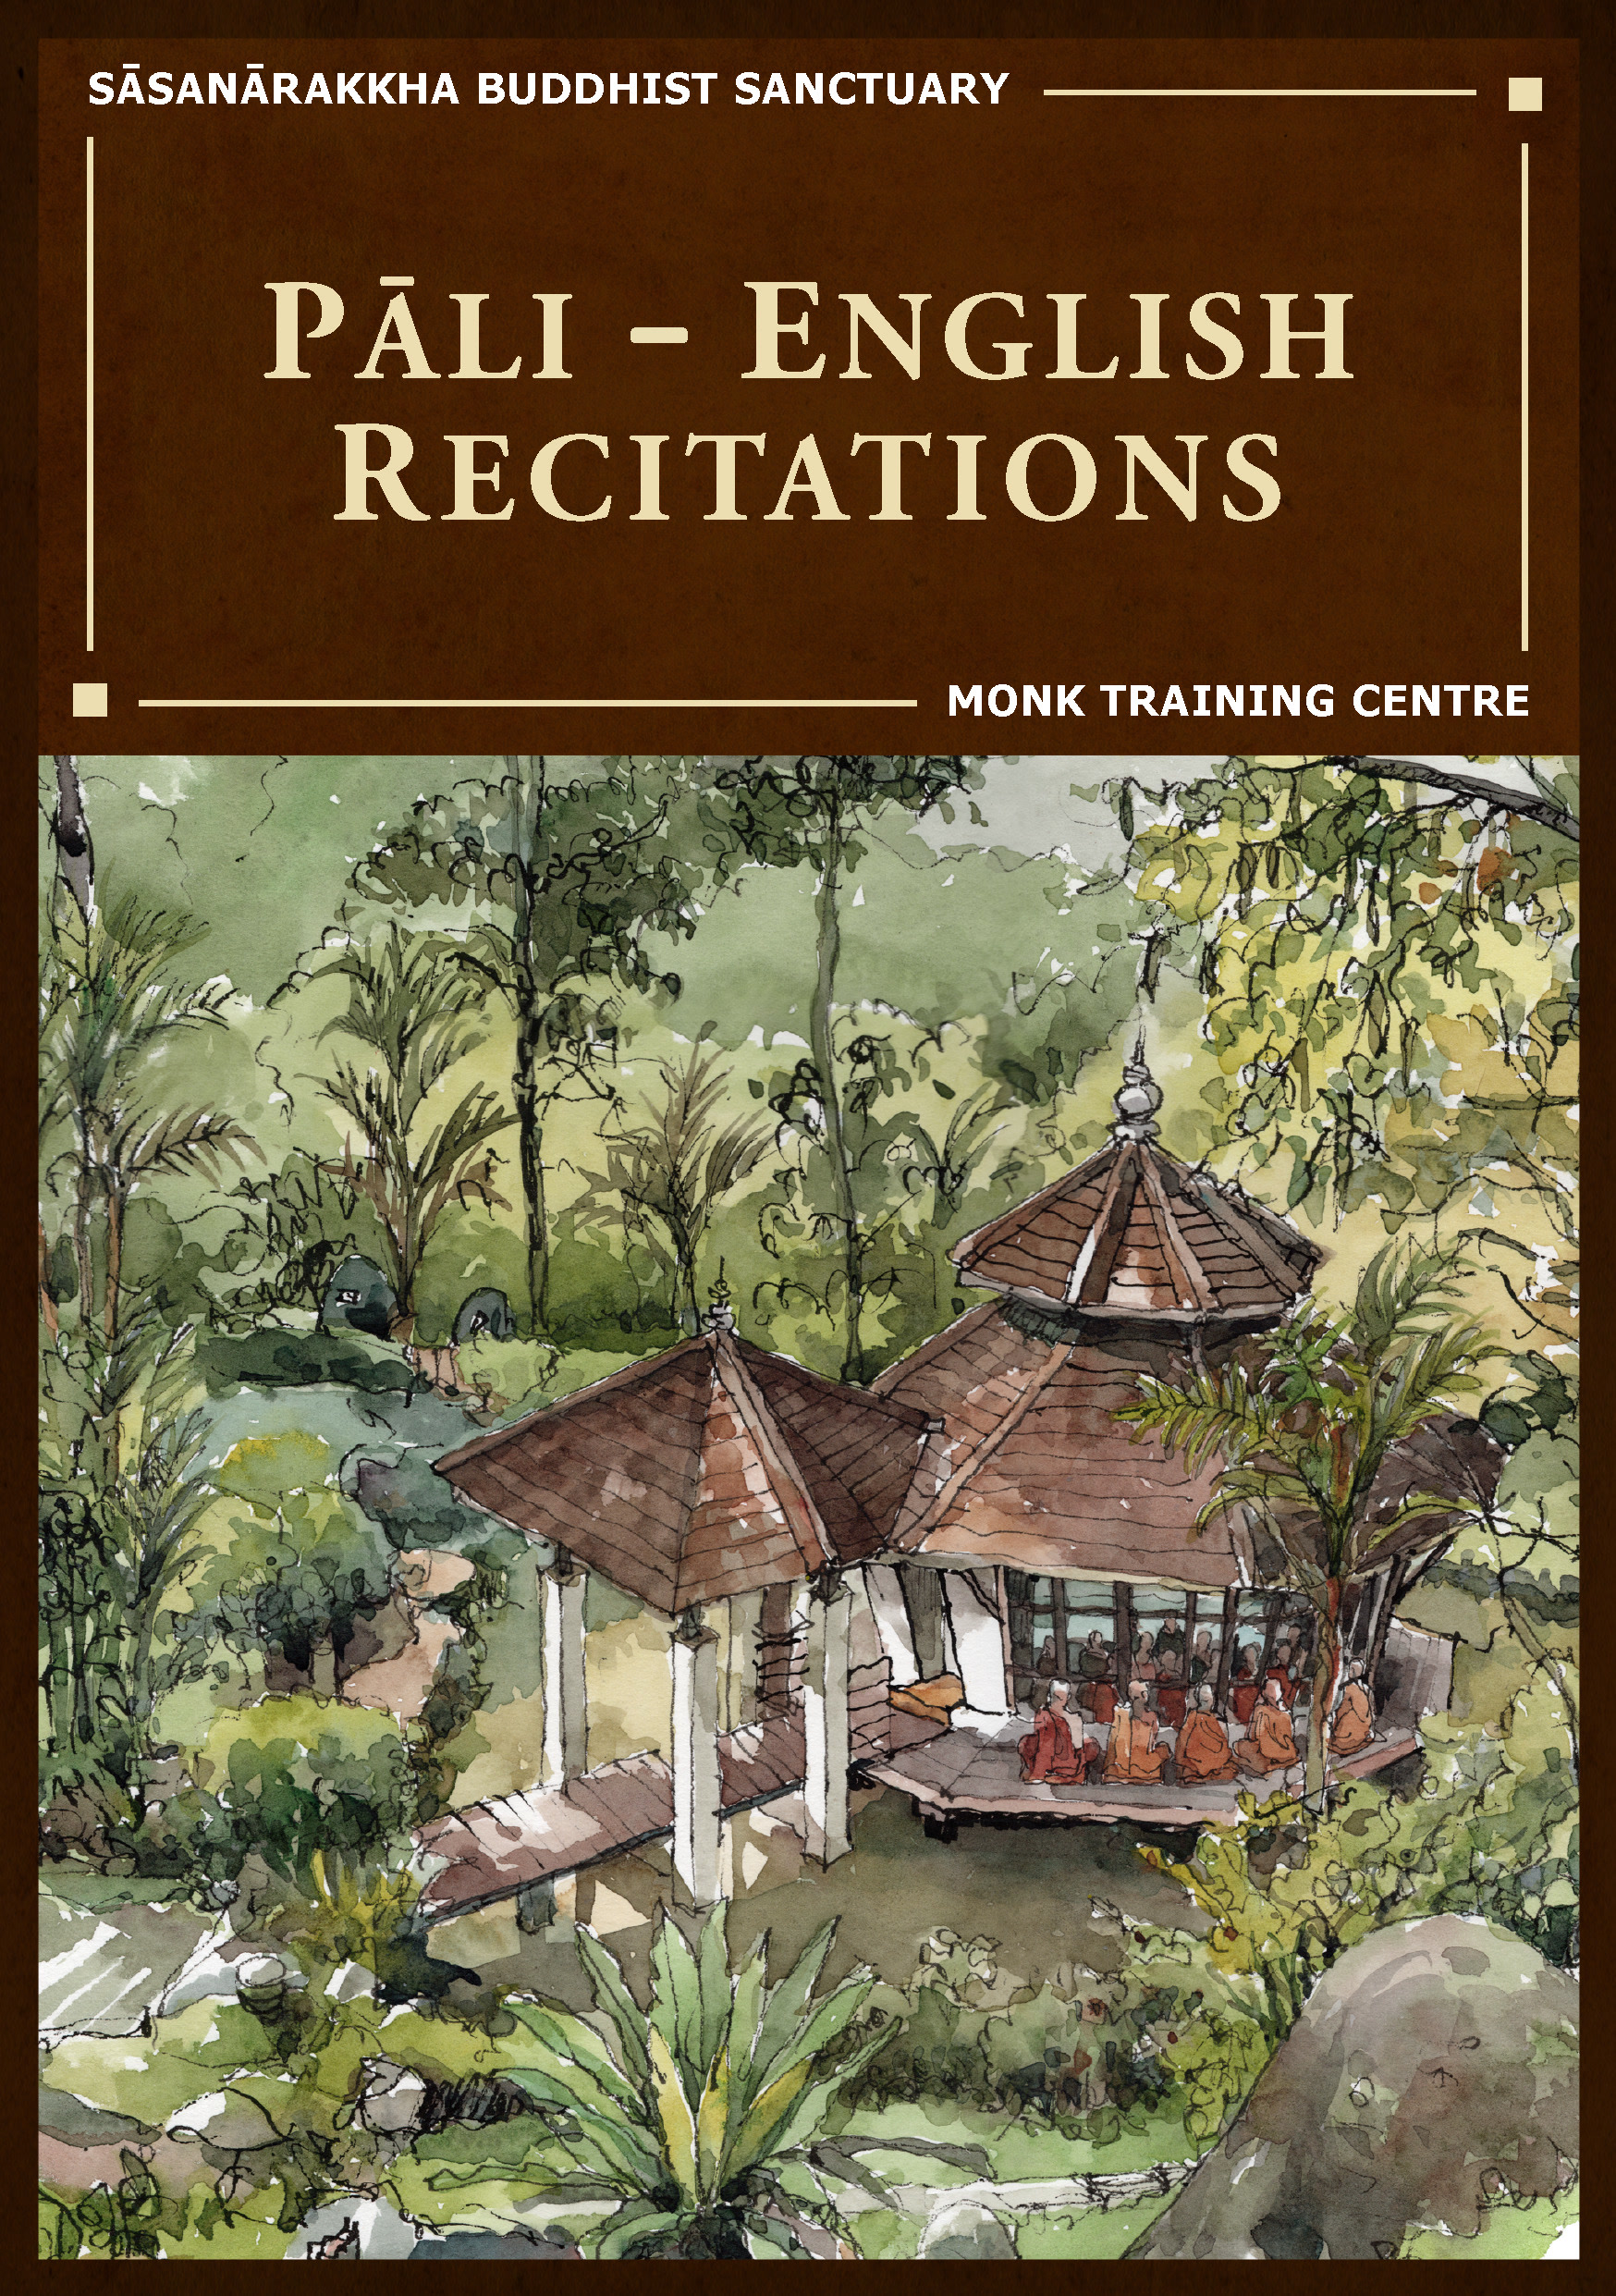
\includegraphics[height=\paperheight]{./assets/images/A5/front_cover_compressed_A5.jpg}}
\fi

\ifninebythirteenversion
  \photoFullBleed{./assets/images/9x13/front_cover_9x13.png}
  \photoFullBleed{robe_divider_left_9x13.png}
  \photoFullBleed{robe_divider_right_9x13.png}
\fi

\ifbfiveversion
  \photoFullBleed{./assets/images/B5/front_cover_B5.png}
  \photoFullBleed{robe_divider_left_B5.png}
  \photoFullBleed{robe_divider_right_B5.png}
\fi

% Title page, copyright, acknowledgments
\pagestyle{empty}
\input{./tex/titlepage.tex}
\input{./tex/copyright.tex}
\input{./tex/acknowledgments.tex}

% Table of contents, schedule, purpose and benefits, abbreviations
\cleartorecto
\pagestyle{toponerow-frontmatter}
\chapterstyle{adrasteia-toc}

\pdfbookmark[section]{\contentsname}{toc}
\tableofcontents*

\input{./tex/schedule.tex}
\input{./tex/purpose-and-benefits.tex}
\input{./tex/abbreviations.tex}

\chapterstyle{adrasteia-frontmatter}

% Main matter
\mainmatter
\pagestyle{toponerow}

\cleartorecto

% Chapters
{\raggedright
	\input{./tex/recitations/homage.tex}
	\input{./tex/recitations/verses.tex}
	\input{./tex/recitations/teachings.tex}
	\input{./tex/recitations/reflections.tex}
	\input{./tex/recitations/cardinal-discourses.tex}
	\input{./tex/recitations/thanksgiving-recitations.tex}
	\input{./tex/recitations/protective-recitations.tex}
	\input{./tex/recitations/funeral-recitations.tex}
	\input{./tex/recitations/sharing-of-merits.tex}
}

% Appendix
\appendix
\input{./tex/appendix.tex}
\input{./tex/refuge-trainings.tex}
\input{./tex/phonetics-pronunciation.tex}
\input{./tex/guidelines.tex}

% Back matter
\backmatter
\printpagenotes % Print endnotes
\input{./tex/copyright-details.tex}

\ifbfiveversion
  \includepdf[pages=-,pagecommand={\thispagestyle{empty}}]{assets/images/graphics/donor-list.pdf}
  \photoFullBleed{robe_divider_left_B5.png}
  \photoFullBleed{robe_divider_right_B5.png}
\fi

\ifninebythirteenversion
  \photoFullBleed{robe_divider_left_9x13.png}
  \photoFullBleed{robe_divider_right_9x13.png}
\fi

\emptyUntilEven % Add blank page if necessary

\ifdigitalversion
  \clearpage
  \digitalCover{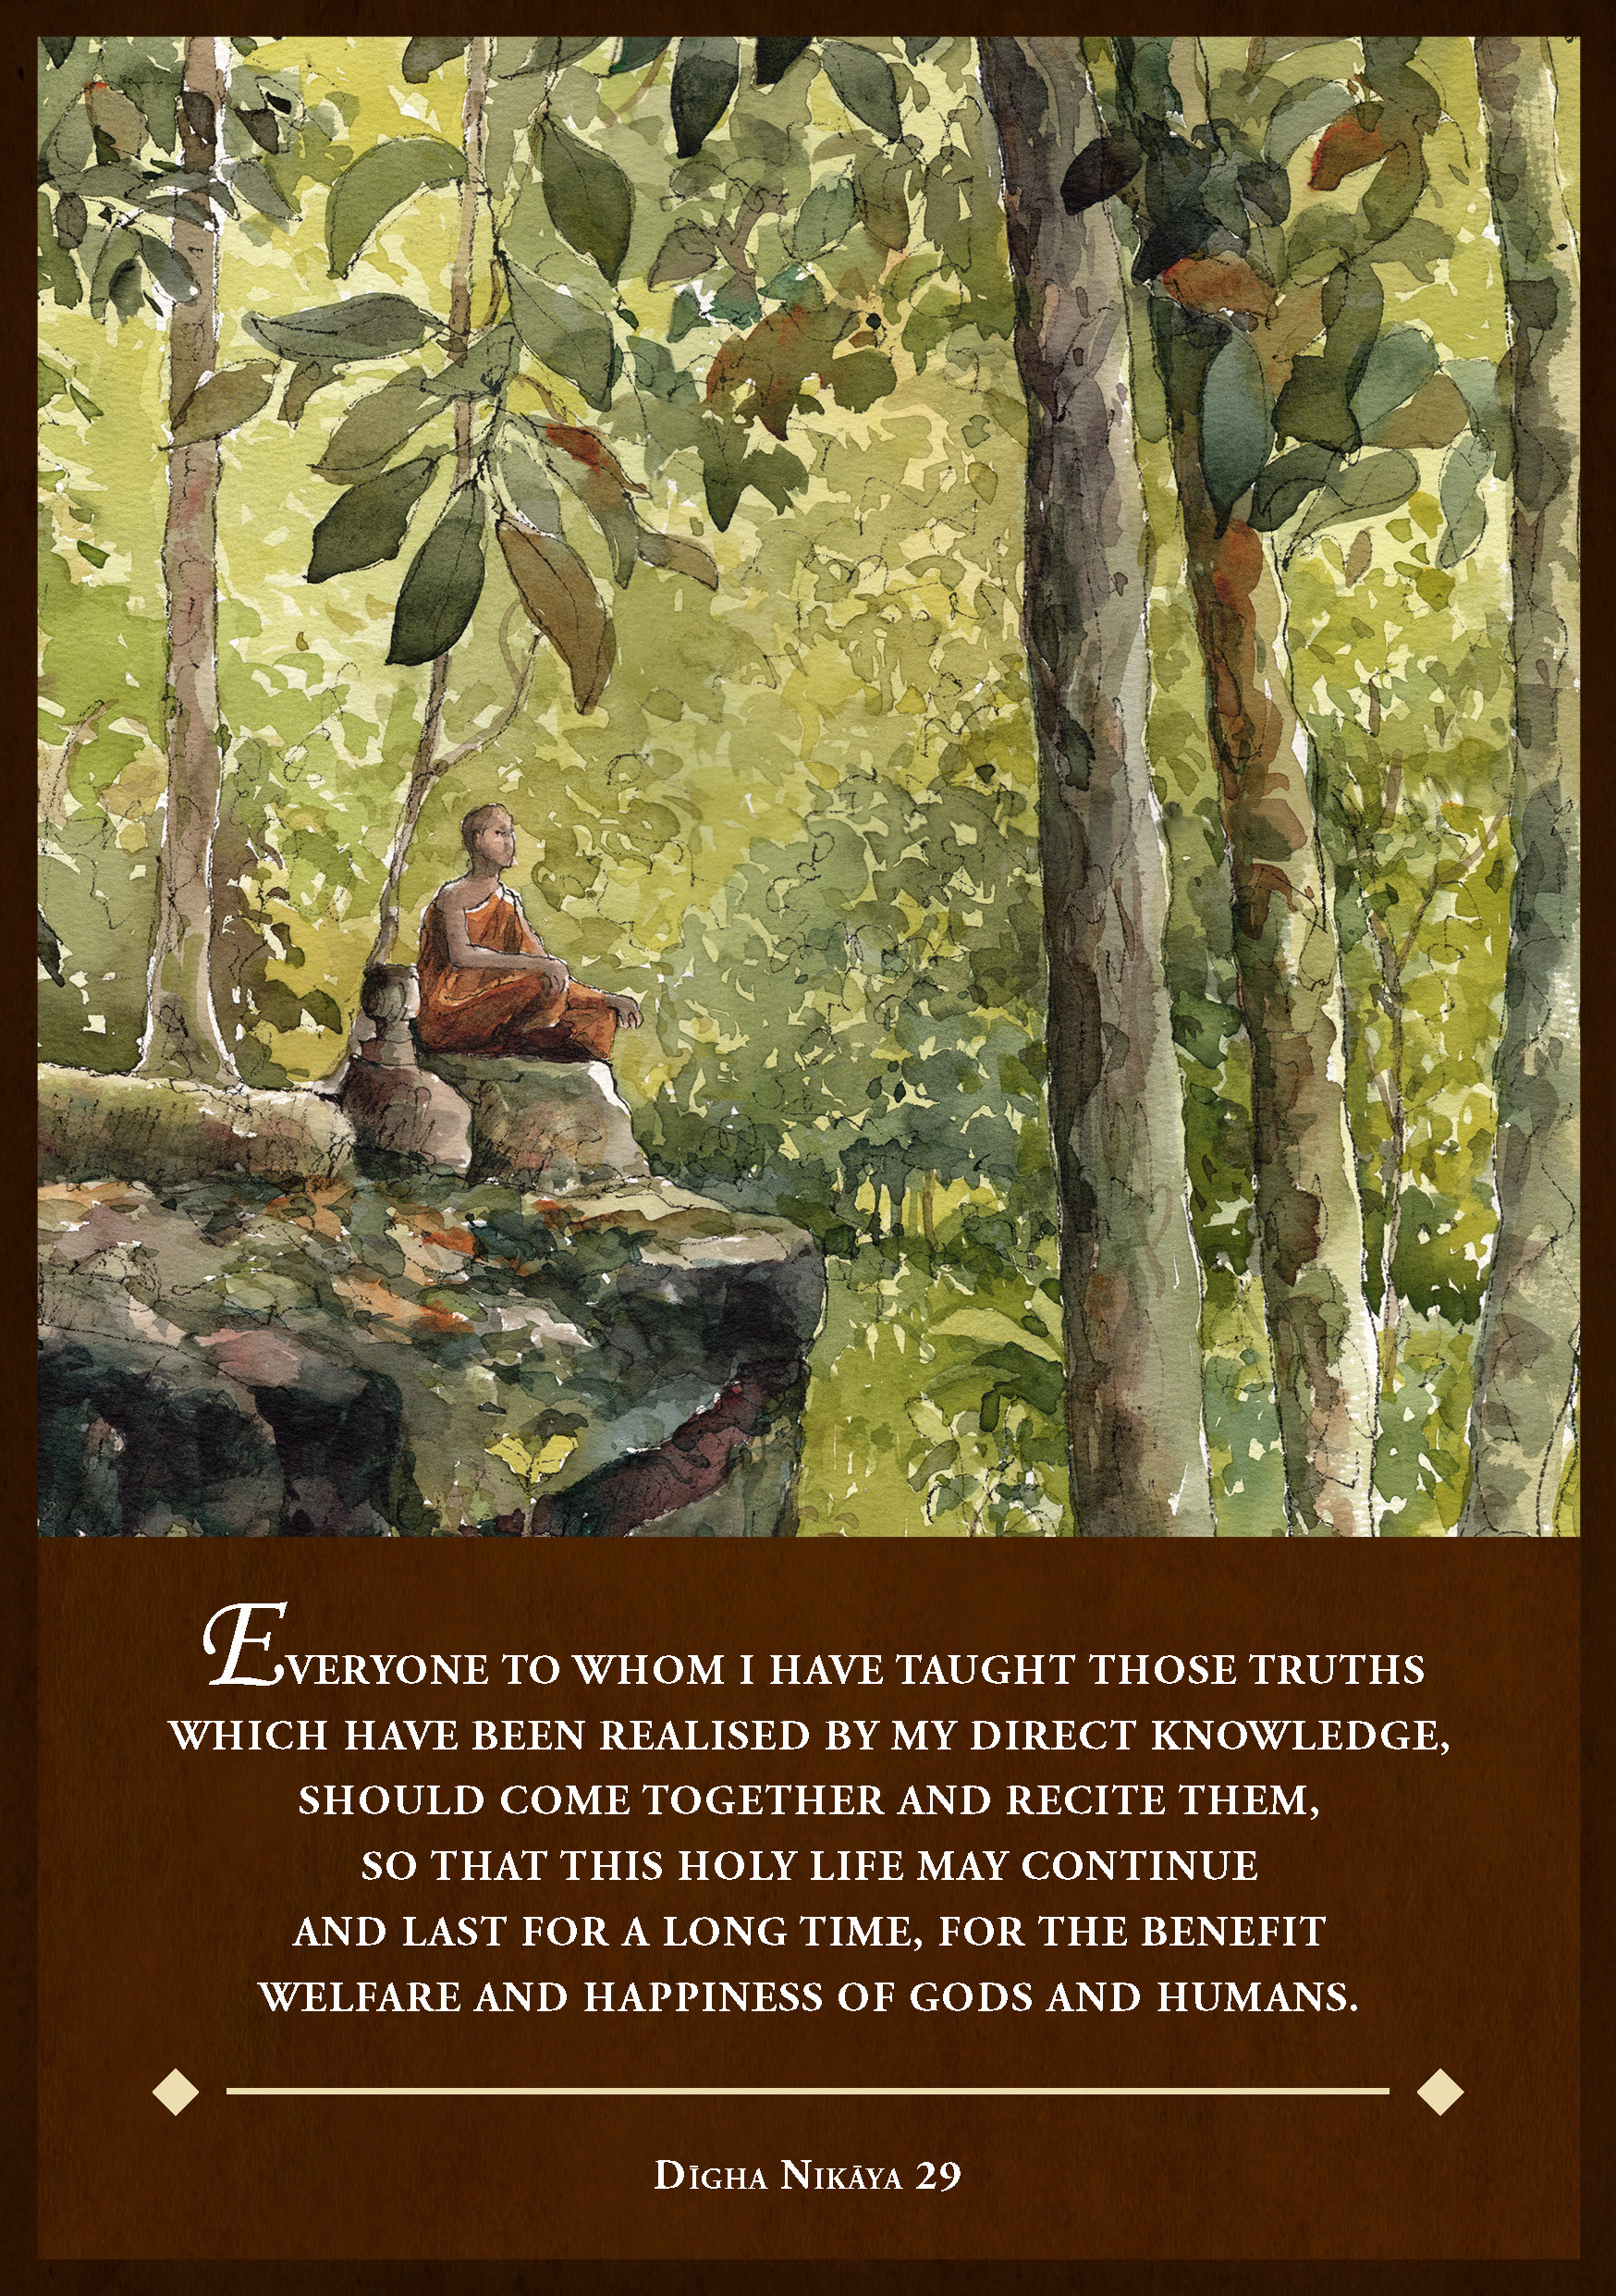
\includegraphics[height=\paperheight]{./assets/images/A5/back_cover_compressed_A5.jpg}}
\fi

\ifninebythirteenversion
  \photoFullBleed{./assets/images/9x13/back_cover_9x13.png}
\fi

\ifbfiveversion
  \photoFullBleed{./assets/images/B5/back_cover_B5.png}
\fi

\end{document}
'
% Possible VALUE:
%   - afiveVersion —  A5 formatted
%   - ninebythirteenVersion —  9x13cm custom formatted
%   - bfiveVersion —  B5 formatted
% \listfiles
\ifdefined\papersizeoption
\else
  \newcommand{\papersizeoption}{bfiveVersion}
\fi
\typeout{Set \protect\papersizeoption{} to \papersizeoption}

% Add hyperlinks and images, to be used with afiveVersion \papersizeoption
% Build command:
% '\newcommand{\papersizeoption}{afiveVersion}\newcommand{\isdigitalversion}{}% Set paper variant
% Build command '\newcommand{\papersizeoption}{VALUE}\input{main.tex}'
% Possible VALUE:
%   - afiveVersion —  A5 formatted
%   - ninebythirteenVersion —  9x13cm custom formatted
%   - bfiveVersion —  B5 formatted
% \listfiles
\ifdefined\papersizeoption
\else
  \newcommand{\papersizeoption}{bfiveVersion}
\fi
\typeout{Set \protect\papersizeoption{} to \papersizeoption}

% Add hyperlinks and images, to be used with afiveVersion \papersizeoption
% Build command:
% '\newcommand{\papersizeoption}{afiveVersion}\newcommand{\isdigitalversion}{}\input{main.tex}'
\ifdefined\isdigitalversion
  \newcommand{\digitaloption}{digitalVersion}
\else
  \newcommand{\digitaloption}{}
\fi
\typeout{Set \protect\digitaloption{} to \digitaloption}

% todo ask bergen to make showtims a togglable condition for b5 and 9x13 only

\documentclass[
  final,
  babelLanguage=british,
  showtrims,
  \papersizeoption,
  \digitaloption,
]{anecdote}

% Define graphics path for images
\graphicspath{
  {./assets/images/A5}
  {./assets/images/9x13}
  {./assets/images/B5}
  {./assets/images/graphics}
}

% Loads formatting for selected ddocument class
\ifninebythirteenversion \usepackage{9x13} \fi
\ifafiveversion \usepackage{A5} \fi
\ifbfiveversion \usepackage{B5} \fi

% Set metadata for the document
\title{SBS Pāli-English Recitations}
\subtitle{Monk Training Centre}
\author{SBS Monk Training Centre}
\publisher{Sāsanārakkha Buddhist Sanctuary}
\date{2021-10-30}
\editionInfo{\textit{First Edition}, 2025} % And last edition. Don't call Pāladhammika.
\newcommand{\MyISBN}{} % default empty

\ifbfiveversion
  \renewcommand{\MyISBN}{978-629-97831-1-4}
\fi
\ifninebythirteenversion
  \renewcommand{\MyISBN}{978-629-97831-2-1}
\fi

\ISBN{\MyISBN}

% Set metadata for PDF properties
\hypersetup{
  pdftitle={\thetitle},
  pdfauthor={\theauthor},
  pdfcopyright={Copyright (C) 2025, \thePublisher},
  pdfsubject={},
  pdfkeywords={},
  pdflicenseurl={https://creativecommons.org/licenses/by-nc-nd/4.0/},
  pdfcontacturl={},
  pdflang={en},
}

% Load further packages
\RequirePackage[yyyymmdd,hhmmss]{datetime} % Adds the time to version creation

\makepagenote
\continuousnotenums % Ensure continuous endnote numbering

% Define hyphenation exceptions and corrections
\hyphenation{London re-lin-quishes de-ter-mines}

\ifdigitalversion
  \openany
\fi

% Begin document
\begin{document}

% Front matter
\frontmatter

% Digital version cover
\ifdigitalversion
	\digitalCover{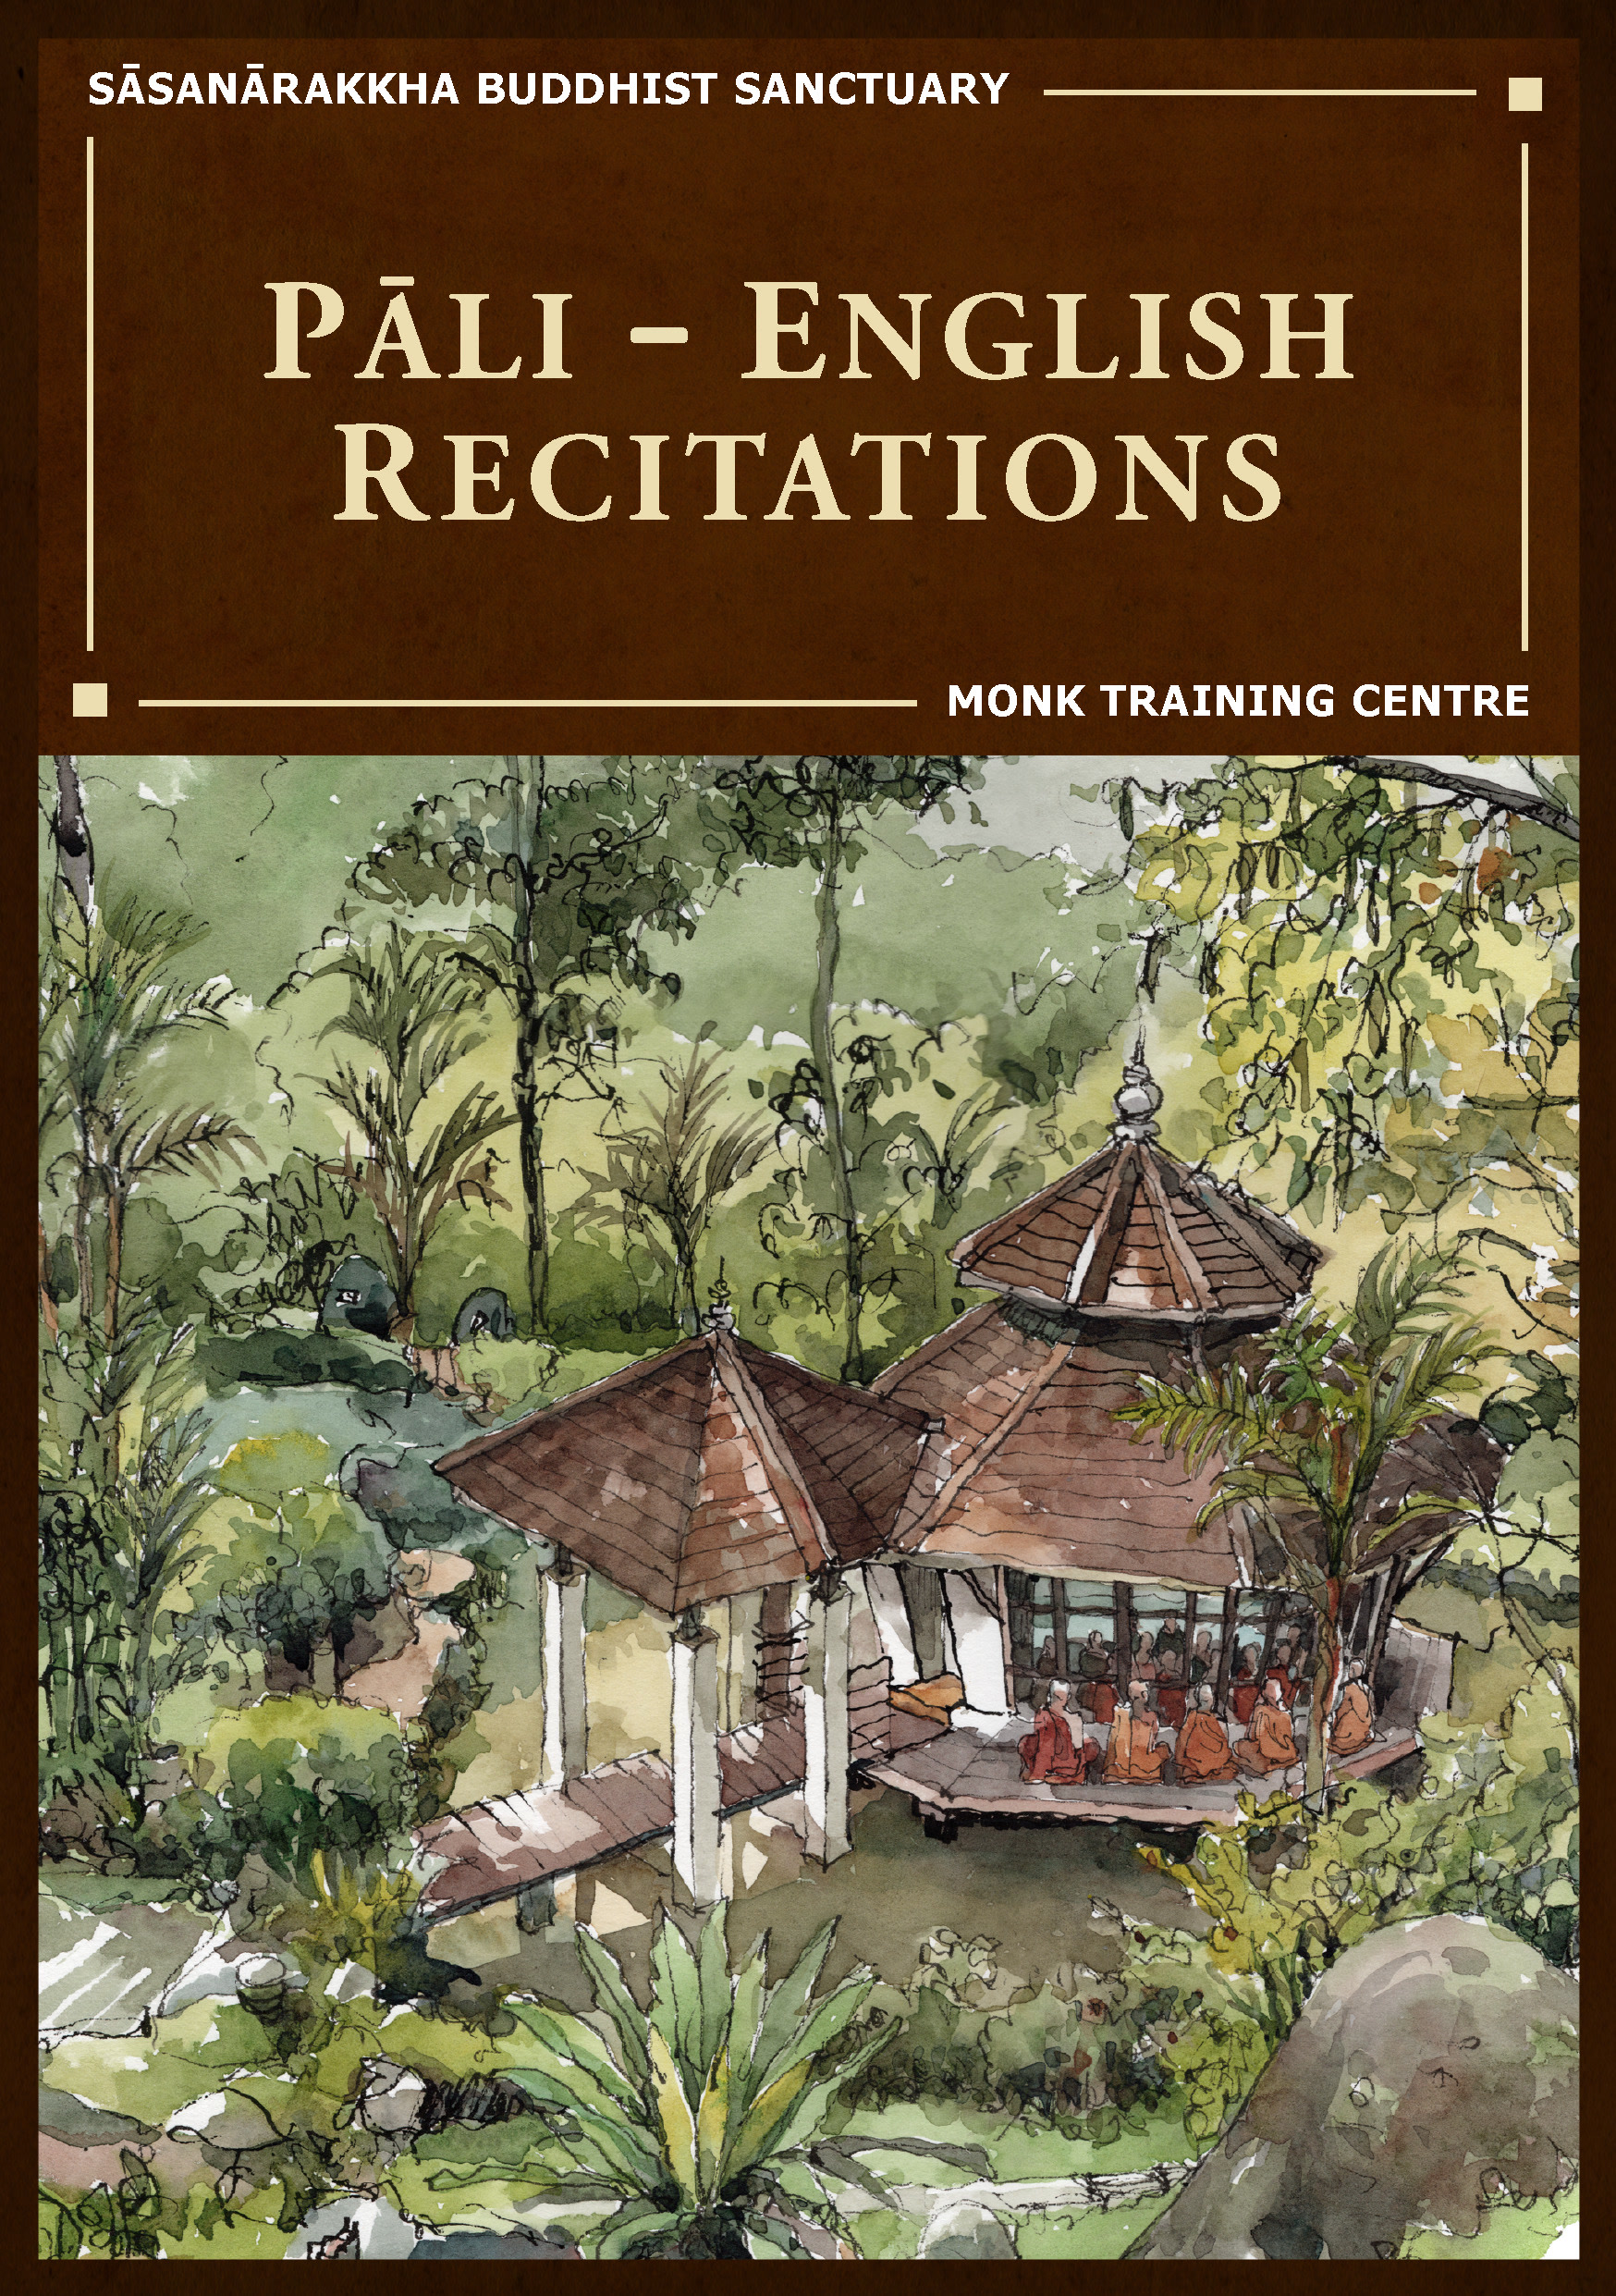
\includegraphics[height=\paperheight]{./assets/images/A5/front_cover_compressed_A5.jpg}}
\fi

\ifninebythirteenversion
  \photoFullBleed{./assets/images/9x13/front_cover_9x13.png}
  \photoFullBleed{robe_divider_left_9x13.png}
  \photoFullBleed{robe_divider_right_9x13.png}
\fi

\ifbfiveversion
  \photoFullBleed{./assets/images/B5/front_cover_B5.png}
  \photoFullBleed{robe_divider_left_B5.png}
  \photoFullBleed{robe_divider_right_B5.png}
\fi

% Title page, copyright, acknowledgments
\pagestyle{empty}
\input{./tex/titlepage.tex}
\input{./tex/copyright.tex}
\input{./tex/acknowledgments.tex}

% Table of contents, schedule, purpose and benefits, abbreviations
\cleartorecto
\pagestyle{toponerow-frontmatter}
\chapterstyle{adrasteia-toc}

\pdfbookmark[section]{\contentsname}{toc}
\tableofcontents*

\input{./tex/schedule.tex}
\input{./tex/purpose-and-benefits.tex}
\input{./tex/abbreviations.tex}

\chapterstyle{adrasteia-frontmatter}

% Main matter
\mainmatter
\pagestyle{toponerow}

\cleartorecto

% Chapters
{\raggedright
	\input{./tex/recitations/homage.tex}
	\input{./tex/recitations/verses.tex}
	\input{./tex/recitations/teachings.tex}
	\input{./tex/recitations/reflections.tex}
	\input{./tex/recitations/cardinal-discourses.tex}
	\input{./tex/recitations/thanksgiving-recitations.tex}
	\input{./tex/recitations/protective-recitations.tex}
	\input{./tex/recitations/funeral-recitations.tex}
	\input{./tex/recitations/sharing-of-merits.tex}
}

% Appendix
\appendix
\input{./tex/appendix.tex}
\input{./tex/refuge-trainings.tex}
\input{./tex/phonetics-pronunciation.tex}
\input{./tex/guidelines.tex}

% Back matter
\backmatter
\printpagenotes % Print endnotes
\input{./tex/copyright-details.tex}

\ifbfiveversion
  \includepdf[pages=-,pagecommand={\thispagestyle{empty}}]{assets/images/graphics/donor-list.pdf}
  \photoFullBleed{robe_divider_left_B5.png}
  \photoFullBleed{robe_divider_right_B5.png}
\fi

\ifninebythirteenversion
  \photoFullBleed{robe_divider_left_9x13.png}
  \photoFullBleed{robe_divider_right_9x13.png}
\fi

\emptyUntilEven % Add blank page if necessary

\ifdigitalversion
  \clearpage
  \digitalCover{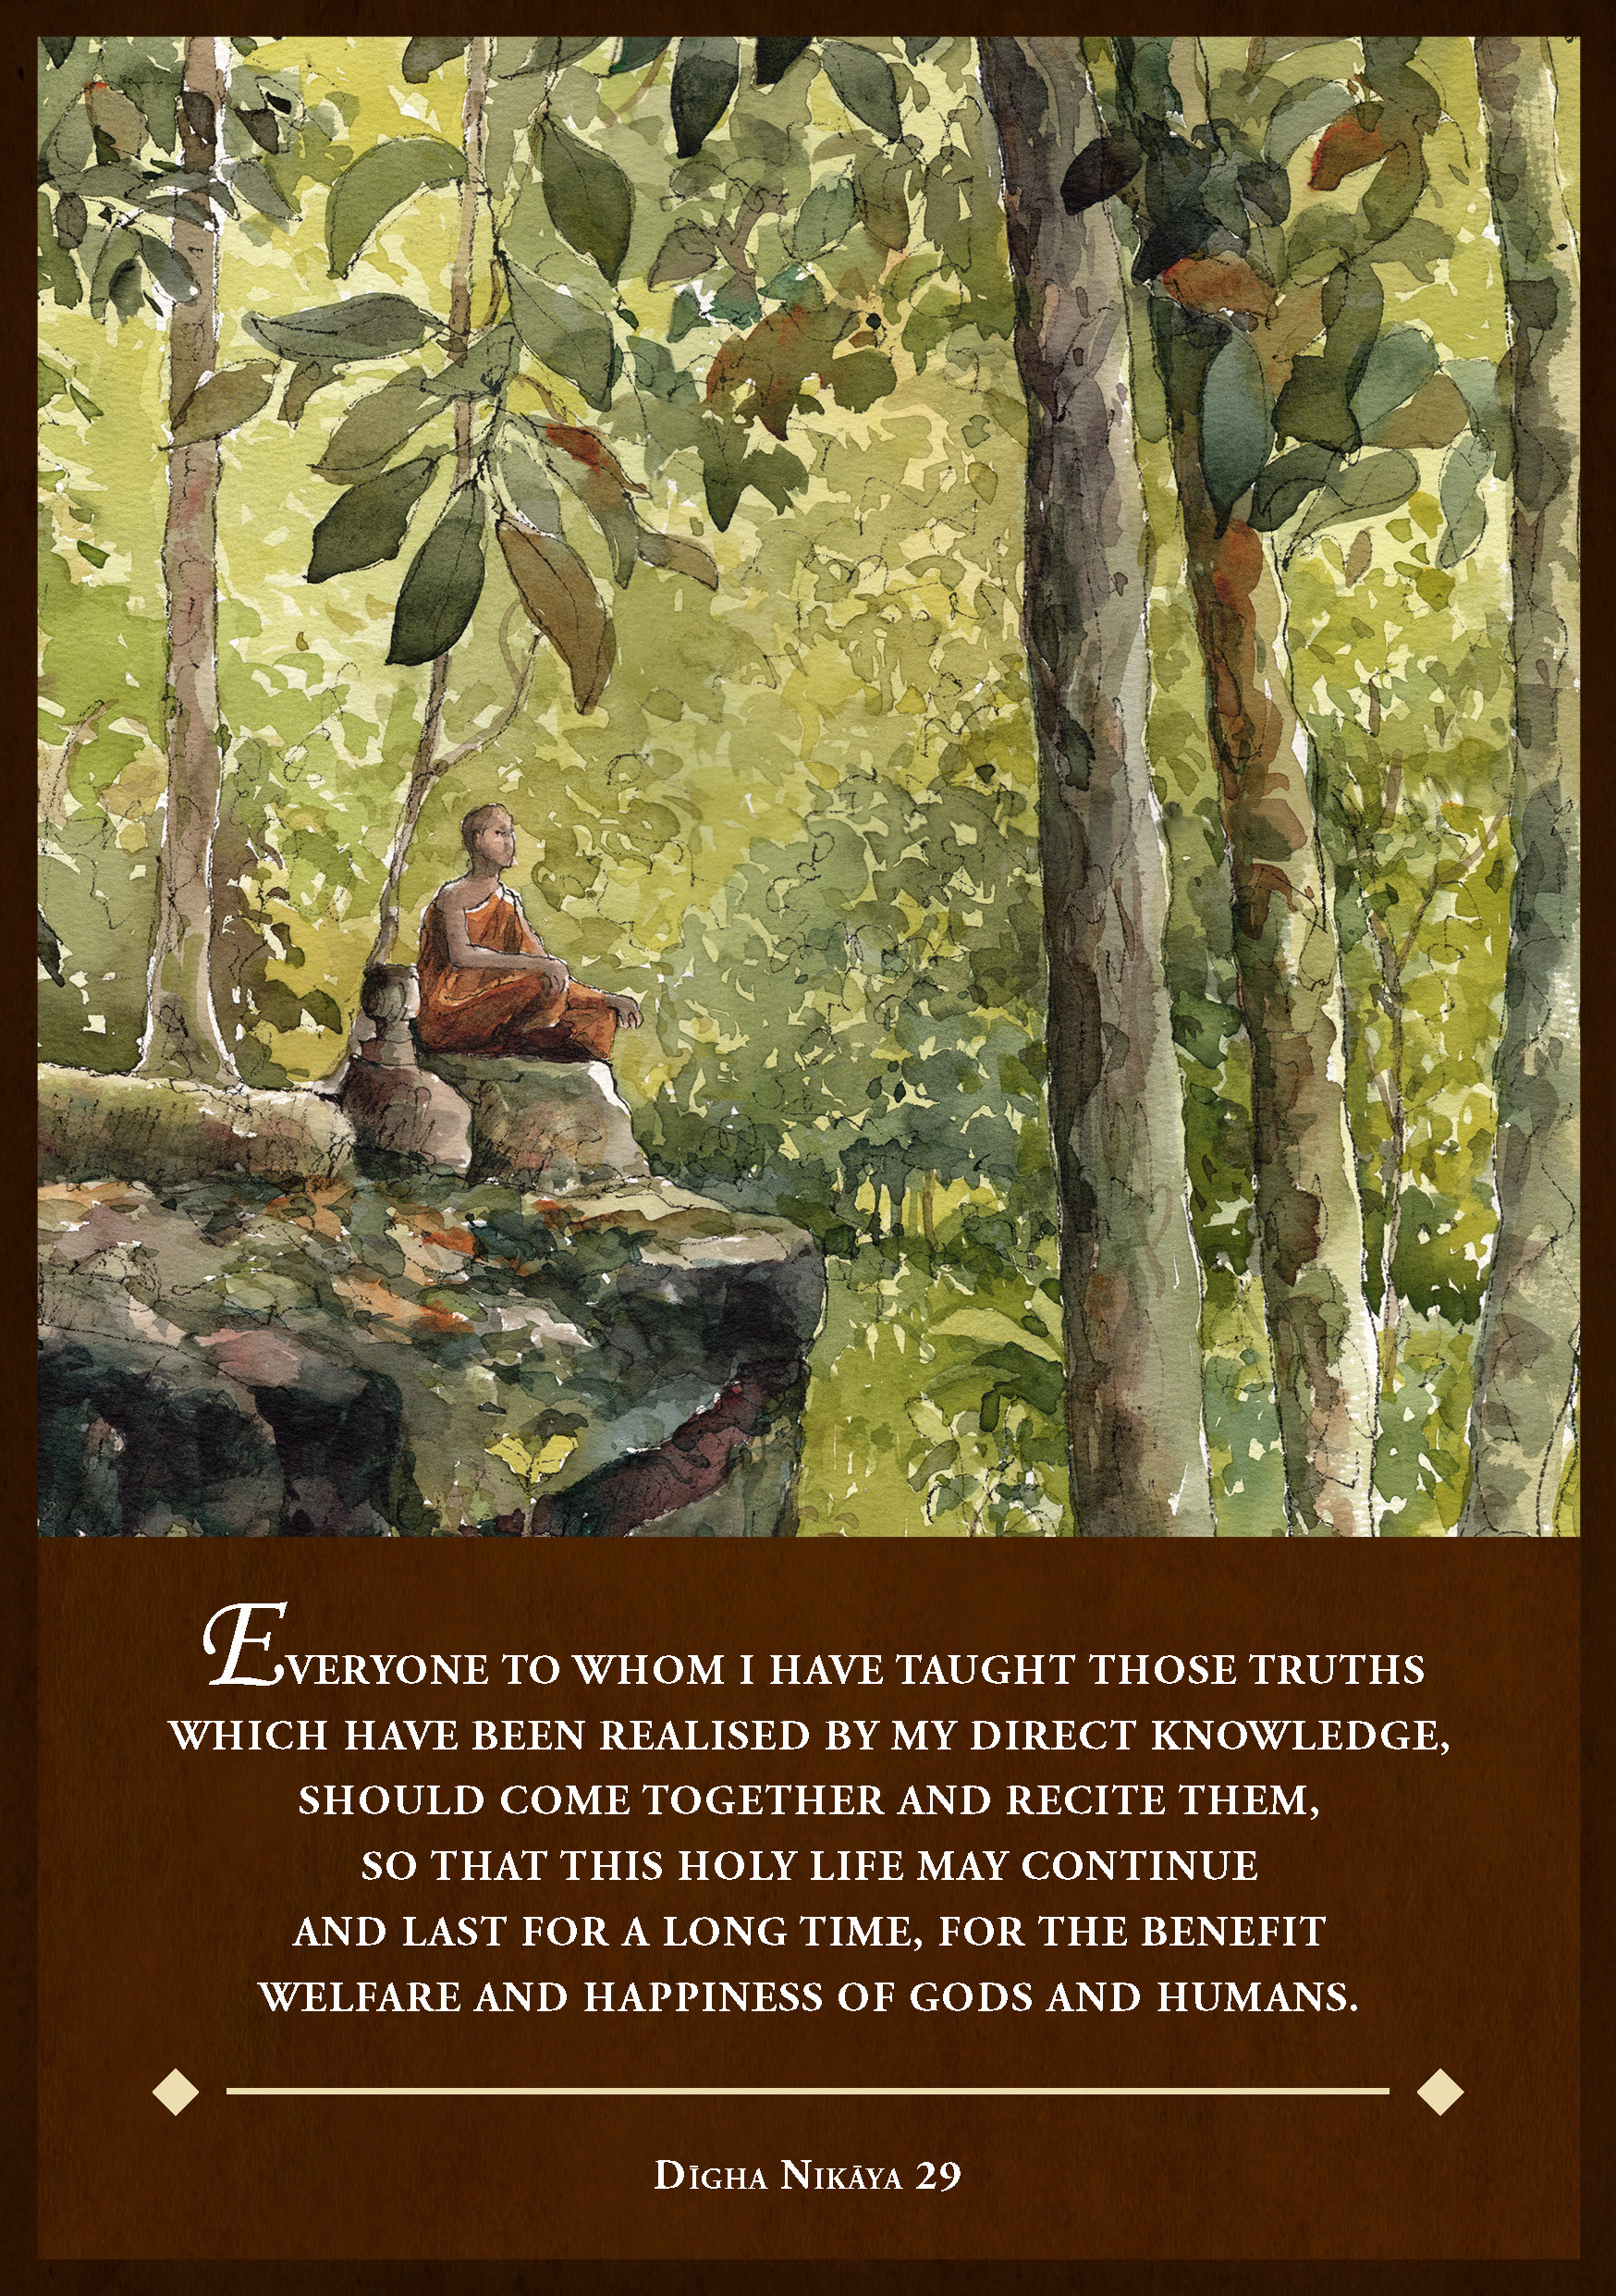
\includegraphics[height=\paperheight]{./assets/images/A5/back_cover_compressed_A5.jpg}}
\fi

\ifninebythirteenversion
  \photoFullBleed{./assets/images/9x13/back_cover_9x13.png}
\fi

\ifbfiveversion
  \photoFullBleed{./assets/images/B5/back_cover_B5.png}
\fi

\end{document}
'
\ifdefined\isdigitalversion
  \newcommand{\digitaloption}{digitalVersion}
\else
  \newcommand{\digitaloption}{}
\fi
\typeout{Set \protect\digitaloption{} to \digitaloption}

% todo ask bergen to make showtims a togglable condition for b5 and 9x13 only

\documentclass[
  final,
  babelLanguage=british,
  showtrims,
  \papersizeoption,
  \digitaloption,
]{anecdote}

% Define graphics path for images
\graphicspath{
  {./assets/images/A5}
  {./assets/images/9x13}
  {./assets/images/B5}
  {./assets/images/graphics}
}

% Loads formatting for selected ddocument class
\ifninebythirteenversion \usepackage{9x13} \fi
\ifafiveversion \usepackage{A5} \fi
\ifbfiveversion \usepackage{B5} \fi

% Set metadata for the document
\title{SBS Pāli-English Recitations}
\subtitle{Monk Training Centre}
\author{SBS Monk Training Centre}
\publisher{Sāsanārakkha Buddhist Sanctuary}
\date{2021-10-30}
\editionInfo{\textit{First Edition}, 2025} % And last edition. Don't call Pāladhammika.
\newcommand{\MyISBN}{} % default empty

\ifbfiveversion
  \renewcommand{\MyISBN}{978-629-97831-1-4}
\fi
\ifninebythirteenversion
  \renewcommand{\MyISBN}{978-629-97831-2-1}
\fi

\ISBN{\MyISBN}

% Set metadata for PDF properties
\hypersetup{
  pdftitle={\thetitle},
  pdfauthor={\theauthor},
  pdfcopyright={Copyright (C) 2025, \thePublisher},
  pdfsubject={},
  pdfkeywords={},
  pdflicenseurl={https://creativecommons.org/licenses/by-nc-nd/4.0/},
  pdfcontacturl={},
  pdflang={en},
}

% Load further packages
\RequirePackage[yyyymmdd,hhmmss]{datetime} % Adds the time to version creation

\makepagenote
\continuousnotenums % Ensure continuous endnote numbering

% Define hyphenation exceptions and corrections
\hyphenation{London re-lin-quishes de-ter-mines}

\ifdigitalversion
  \openany
\fi

% Begin document
\begin{document}

% Front matter
\frontmatter

% Digital version cover
\ifdigitalversion
	\digitalCover{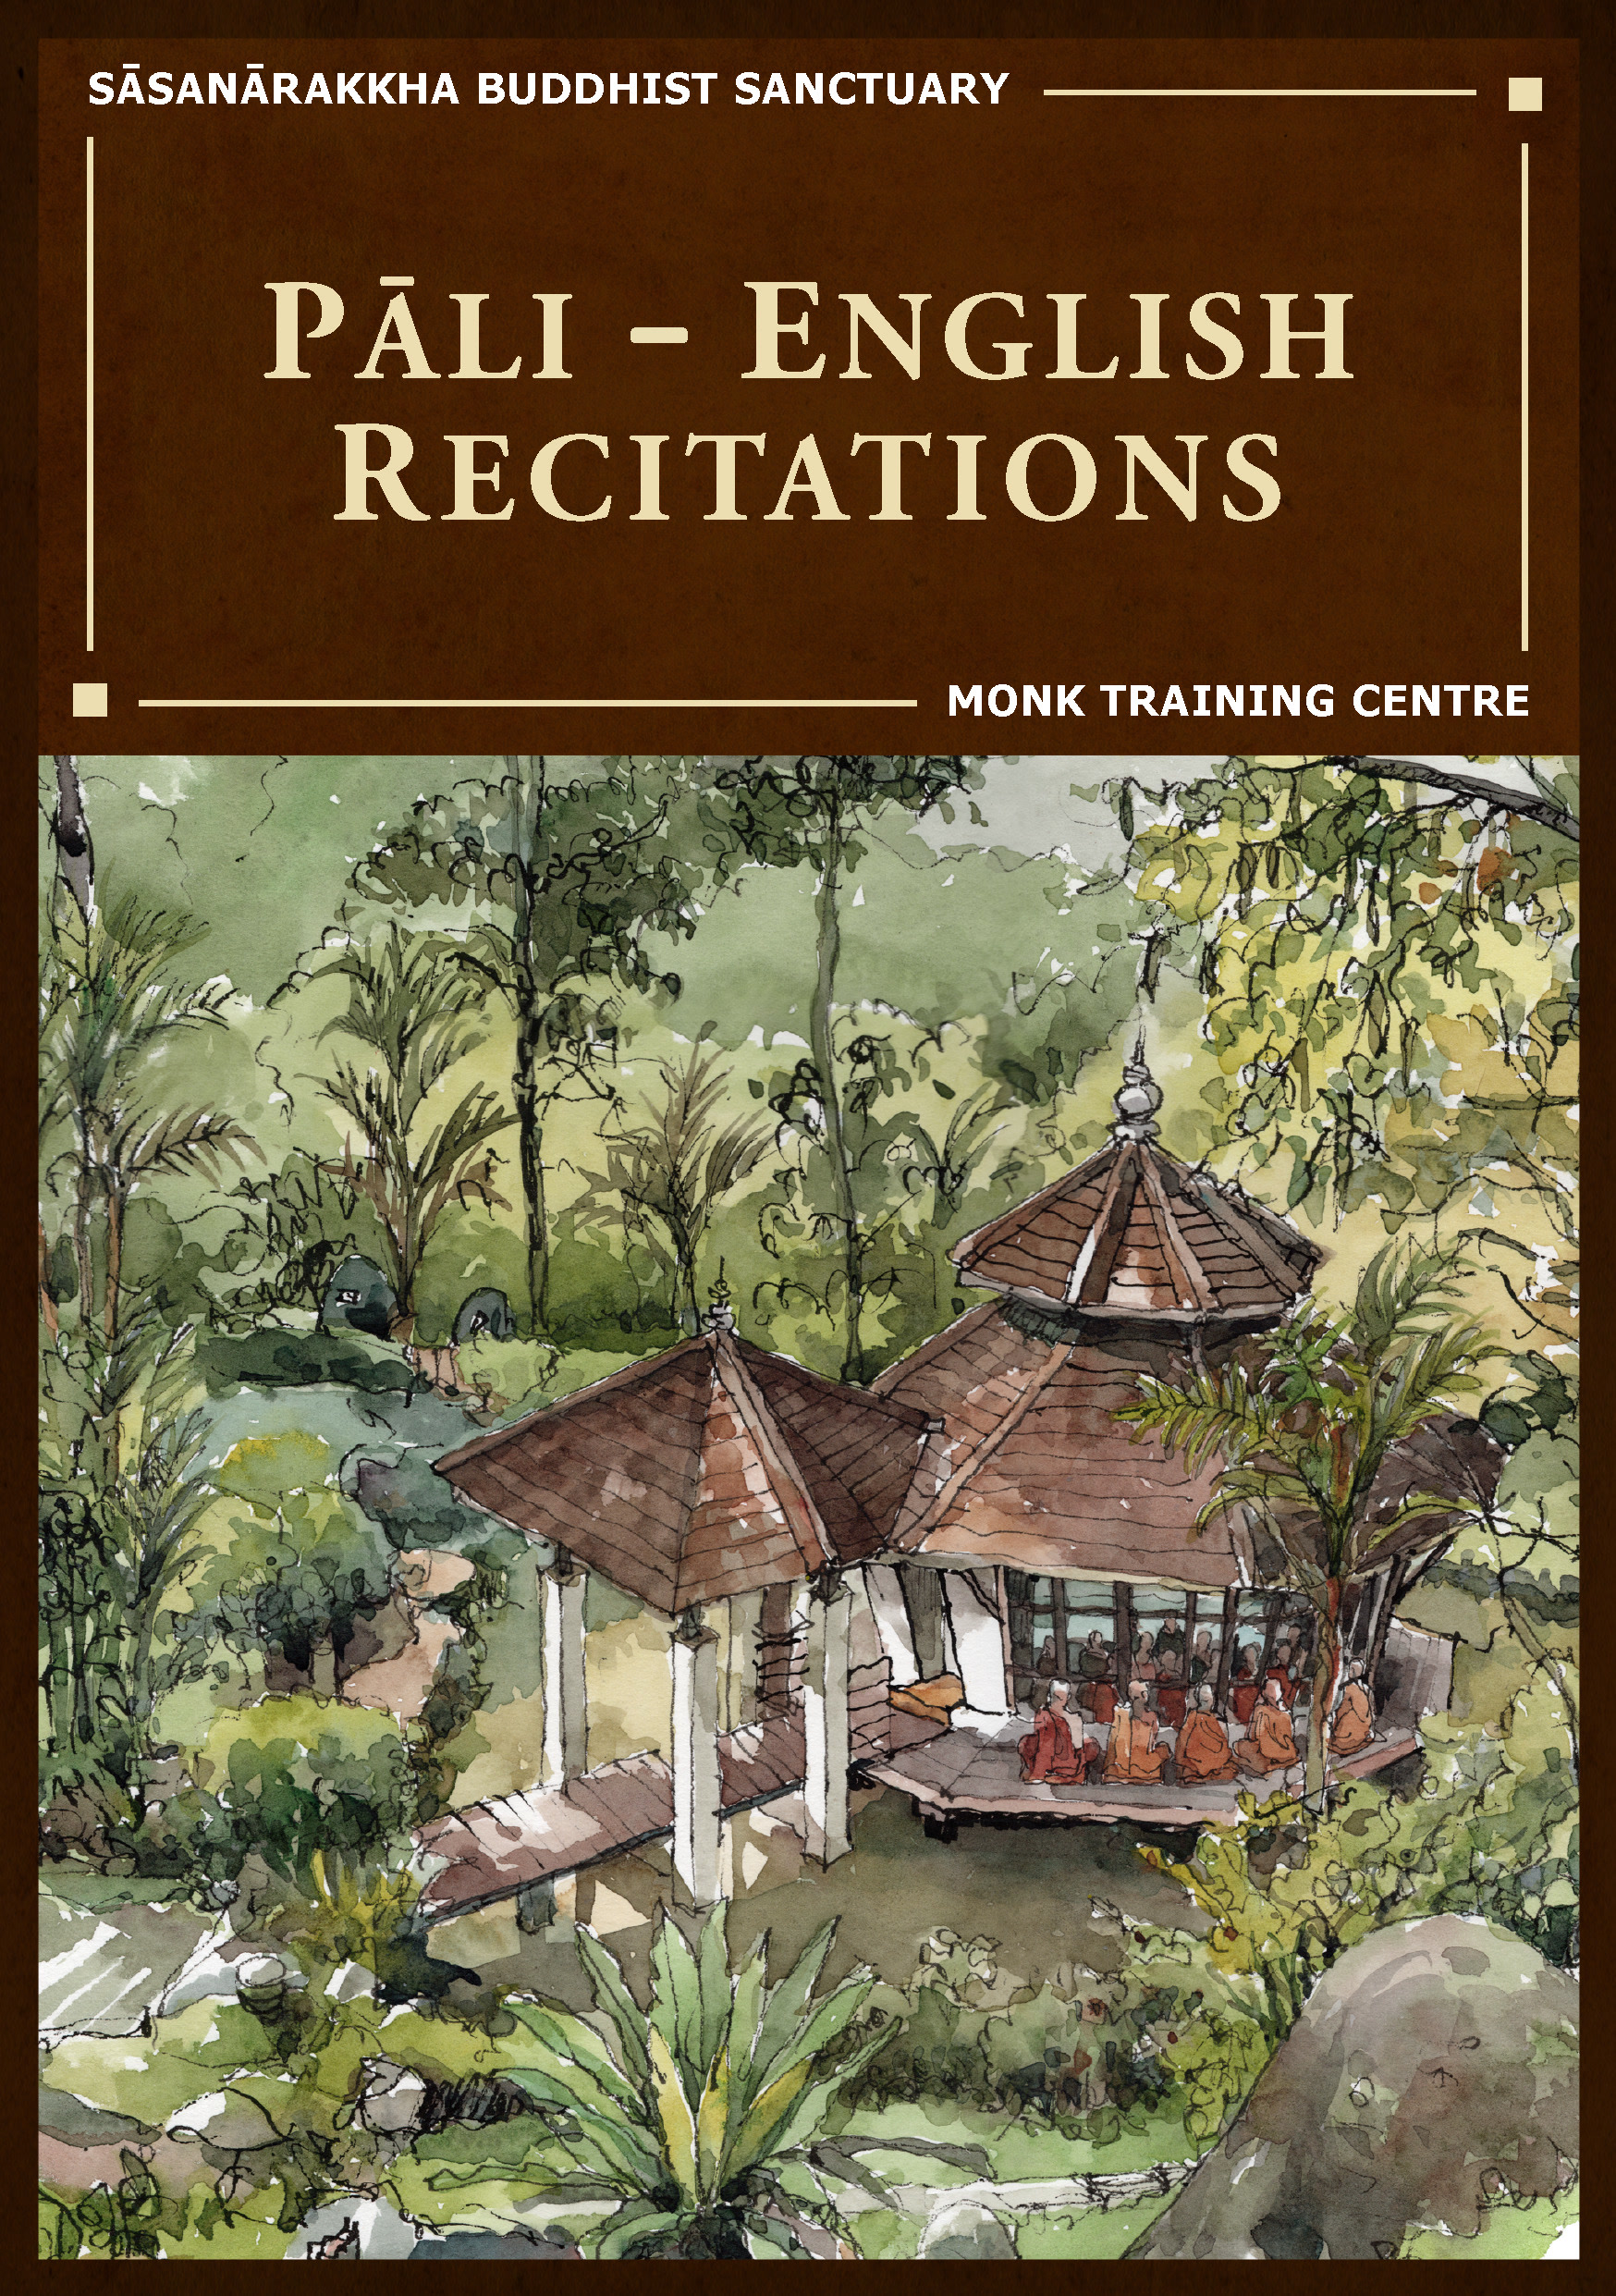
\includegraphics[height=\paperheight]{./assets/images/A5/front_cover_compressed_A5.jpg}}
\fi

\ifninebythirteenversion
  \photoFullBleed{./assets/images/9x13/front_cover_9x13.png}
  \photoFullBleed{robe_divider_left_9x13.png}
  \photoFullBleed{robe_divider_right_9x13.png}
\fi

\ifbfiveversion
  \photoFullBleed{./assets/images/B5/front_cover_B5.png}
  \photoFullBleed{robe_divider_left_B5.png}
  \photoFullBleed{robe_divider_right_B5.png}
\fi

% Title page, copyright, acknowledgments
\pagestyle{empty}

\cleartorecto
\thispagestyle{empty}

\vspace*{3em}

{\centering

  \settowidth{\titleLength}{%
    {\Large\chapterTitleFont\textsc{\MakeUppercase{{Pāli-English Recitations}}}}%
  }

  % 'SBS' on title page
  \ifafive {\Huge\fontsize{64}{16}\sbsFont SBS}\\[1.0\baselineskip] \fi
  \ifninebythirteen {\Huge\fontsize{42.5}{11}\sbsFont SBS}\\[1.0\baselineskip] \fi
  \ifbfive {\Huge\fontsize{80}{16}\sbsFont SBS}\\[1.0\baselineskip] \fi

  % 'Monk Training Centre'
  \ifafive \setlength{\xheight}{\heightof{X}}
    {\Huge\chapterTitleFont\textsc{{\thesubtitle\linebreak}}}\\[0.2\baselineskip] \fi
  \ifninebythirteen {\fontsize{16}{14}\chapterTitleFont\textsc{{\thesubtitle\linebreak}}}\\[0.2\baselineskip] \fi
  \ifbfive \setlength{\xheight}{\heightof{X}}
    {\fontsize{30}{14}\chapterTitleFont\textsc{{\thesubtitle\linebreak}}}\\[0.2\baselineskip] \fi

  % Ornament
  \ifafive \raisebox{0.5\xheight}{\pgfornament[color=sbs-brown,width=7cm,scale=1,ydelta=0pt,symmetry=c]{84}}\\[1.4\baselineskip] \fi
  \ifninebythirteen \raisebox{0.5\xheight}{\pgfornament[color=sbs-brown,width=4.5cm,scale=1,ydelta=0pt,symmetry=c]{84}}\\[1.4\baselineskip] \fi
  \ifbfive \raisebox{0.5\xheight}{\pgfornament[color=sbs-brown,width=8.5cm,scale=1,ydelta=0pt,symmetry=c]{84}}\\[1.4\baselineskip] \fi


  % 'Pali-English Recitations'
  \ifafive {\Large\scshape Pāli-English Recitations}\\[2.5\baselineskip] \fi
  \ifninebythirteen {\fontsize{10}{12}\scshape Pāli-English Recitations}\\[2.5\baselineskip] \fi
  \ifbfive {\fontsize{18.5}{12}\scshape Pāli-English Recitations}\\[2.5\baselineskip] \fi

  % Dhamma quote
  {\quote ``In whatever way a bhikkhu recites the Dhamma in detail as he has heard it and learned it, in just that way, in relation to that Dhamma, he experiences inspiration in the meaning and inspiration in the Dhamma. As he does so, joy arises in him. When he is joyful, rapture arises. For one with a rapturous mind, the body becomes tranquil. One tranquil in body feels pleasure. For one feeling pleasure, the mind becomes concentrated.''\\}
  \ifafive \smallskip AN 5.26\\[1.4\baselineskip]\fi
  \ifninebythirteen \smallskip \fontsize{8}{14}\selectfont AN 5.26\\[1.4\baselineskip]\fi
  %% \ifbfive \smallskip \fontsize{8.5}{14}\selectfont AN 5.26\\[1.4\baselineskip]\fi
  \ifbfive \smallskip AN 5.26\\[1.4\baselineskip]\fi
}



\cleartoverso
\thispagestyle{empty}

{%

  \ifafive \fontsize{10}{16}\selectfont \fi
  \ifninebythirteen \fontsize{7.5}{11}\selectfont \fi
  \ifbfive \fontsize{12}{20}\selectfont \fi
  \centering
  \setlength{\parindent}{0pt}%

  \ifafive \vspace{0.5cm} \fi
  \ifninebythirteen \vspace{0.4cm} \fi
  \ifbfive \vspace{0.5cm} \fi

  \copyright\ \thePublisher, 2025\\
  c/o 160, Lorong 3, Jalan Merdeka, 34000 Taiping, Perak, Malaysia\\
  \ifdigital
    \else
  ISBN \theISBN
  \fi

  \ifafive \vspace{0.5cm} \fi
  \ifninebythirteen \vspace{0.3cm} \fi
  \ifbfive \vspace{0.5cm} \fi

  This book is for free distribution only;\\
  it may not be sold.

  \ifafive \vspace{0.5cm} \fi
  \ifninebythirteen \vspace{0.3cm} \fi
  \ifbfive \vspace{0.5cm} \fi

  Download this book as a PDF, EPUB, MOBI, AZW3\\
  at the following address:\\
  \href{https://sasanarakkha.org/recitations}{https://sasanarakkha.org/recitations}

Accompanying audio recordings can be found at:
\href{https://www.youtube.com/SasanarakkhaBuddhistSanctuary}{https://www.youtube.com/SasanarakkhaBuddhistSanctuary}

  \ifafive \vspace{0.5cm} \fi
  \ifninebythirteen \vspace{0.3cm} \fi
  \ifbfive \vspace{0.5cm} \fi

  Project Manager: Ā. Ariyadhammika\\
  Editor: Ā. Pāladhammika\\
  Typesetting: Aj. Gambhiro, Ā. Pāladhammika\\
  Translators: Ā. Aggacitta, Ā. Bodhi, Aj. Kevalī, Ā. Sujāto, M. Walshe\\
  Endnotes: Ā. Ariyadhammika\\
  Watercolor Paintings: Lim Jee Yuan

  \ifafive \vspace{0.5cm} \fi
  \ifninebythirteen \vspace{0.3cm} \fi
  \ifbfive \vspace{0.5cm} \fi

  This work is licensed under a Creative Commons\\
  Attribution-NonCommercial-NoDerivatives 4.0 International~License.

  % Produced with the \LaTeX\ typesetting system,\\
  % set in Libertinus Serif.

  \ifafive  \vspace{0.5cm} \fi
  \ifninebythirteen \vspace{0.3cm} \fi
  \ifbfive \vspace{0.5cm} \fi

  \ifdigital
    This version was created on:\\
    \today \space at \currenttime\\
  \fi

  \ifafive \vspace{0.5cm} \fi
  \ifninebythirteen \vspace{0.15cm} \fi
  \ifbfive \vspace{0.5cm} \fi

  \theEditionInfo

}

\ifdigital

\else

\clearpage

\fi



\cleartorecto
\thispagestyle{empty}

{

  \setlength{\parskip}{10pt}

  \ifafive {\centering\fontsize{16}{25}\selectfont \textsc{We Wish To Gratefully Acknowledge} \par} \fi
  \ifninebythirteen {\centering\fontsize{10}{18}\selectfont \textsc{We Wish To Gratefully Acknowledge} \par} \fi
  \ifbfive {\centering\fontsize{18.5}{25}\selectfont \textsc{We Wish To Gratefully Acknowledge} \par} \fi


  The Saṅghas of Wat Pah Nanachat (WPN), Amaravati, and Abhayagiri for allowing the use of material from their respective chanting books, the late Ven. Dr. Saddhātissa and Mr. Maurice Walshe for their English translations, as well as Ven. Bhikkhu Bodhi for granting permission to use and slightly adapt his translations. Various Saṅgha members of SBS Monk Training Centre, who contributed in the compilation of an interesting selection of chants, as well as for providing countless suggestions to help improve the English translations.

  \linkdest{endnote1-body}
  Additional information on translations, as well as deviations\makeatletter\hyperlink{endnote1-appendix}\Hy@raisedlink{{\pagenote{%
        \hypertarget{endnote1-appendix}{\hyperlink{endnote1-body}{Due to the balanced and inspiring selection of chants, as well as for the sake of compatibility, WPN’s \textit{Buddhist Chanting} (2014) has served as the basis for this book. Over time, suggestions for the inclusion of additional chants, as well as occasional improvements of existing translations were incorporated. Such changes were meticulously marked down in the endnotes of the digital versions of this chanting book, so that someone familiar with the present book can straight away find the relevant differences, which can be useful when visiting a branch monastery of the Ajahn Chah lineage, in order to know in which places to revert to the original version.}}}}}\makeatother\thickspace
  from WPN's \textit{Buddhist Chanting} (2014), have been annotated by Ven. Ariyadhammika in the endnotes.


  \ifninebythirteen \smallskip \else \medskip \fi

  {\centering

    To Āyasmā Aggacitta, the founding father of\\
    Sāsanārakkha Buddhist Sanctuary.

    % \ifninebythirteen \smallskip \else \medskip \fi

    \begin{center}
      \ifafive 
\includegraphics[height=54mm]{sbs_logo_tuck_loon_brown.jpg} \fi
      \ifninebythirteen \clearpage \vspace*{\fill}
 
\includegraphics[height=80mm]{sbs_logo_tuck_loon_brown.jpg} \vspace*{\fill} \fi
      \ifbfive \vspace{1cm} 
\includegraphics[height=70mm]{sbs_logo_tuck_loon_brown.jpg}\fi
    \end{center}
  }
}



% Table of contents, schedule, purpose and benefits, abbreviations
\cleartorecto
\pagestyle{toponerow-frontmatter}
\chapterstyle{adrasteia-toc}

\pdfbookmark[section]{\contentsname}{toc}
\tableofcontents*


\chapter{Recitation Schedule}
\label{schedule}

{\centering

  {\pdfbookmark[2]{Set 1}{set1}\libertinusFont\selectfont\textbf{\textsc{\ifafive\fontsize{18}{12}\fi\ifninebythirteen\fontsize{13}{8.5}\fi\ifbfive\fontsize{22}{18}\fi\selectfont\textls*{Set 1}}}}\\
  \textsc{\ifafive\fontsize{14.4}{28}\fi\ifninebythirteen\fontsize{8.7}{17}\fi\ifbfive\fontsize{16}{33.5}\fi\selectfont
    \hyperref[buddhas-first-exclamation]{The Buddha's First Exclamation} \ifdigital\else\pageref{buddhas-first-exclamation}\fi\\
    \hyperref[wheel-of-dhamma-abridged]{Turning the Wheel of Dhamma} \ifdigital\else\pageref{wheel-of-dhamma-abridged}\fi\\
    \hyperref[true-false-refuges]{Going to True and False Refuges} \ifdigital\else\pageref{true-false-refuges}\fi\\
    \hyperref[four-great-references]{The Four Great References} \ifdigital\else\pageref{four-great-references}\fi\\
    \hyperref[patimokkha-exhortation]{The Pāṭimokkha Exhortation} \ifdigital\else\pageref{patimokkha-exhortation}\fi\\
    \hyperref[buddhas-final-instruction]{The Buddha's Final Instruction} \ifdigital\else\pageref{buddhas-final-instruction}\fi\\
    \hyperref[uddissanadhitthana]{Sharing and Aspirations (Pāli)} \ifdigital\else\pageref{uddissanadhitthana}\fi\\
    \hyperref[closing-homage]{Closing Homage (Pāli-English)} \ifdigital\else\pageref{closing-homage}\fi\\
  }

  \ifafive\vspace{1.0cm}\fi
  \ifninebythirteen\vspace{0.8cm}\fi
  \ifbfive\vspace{1.0cm}\fi

  {\pdfbookmark[2]{Set 2}{set2}\libertinusFont\selectfont\textbf{\textsc{\ifafive\fontsize{18}{12}\fi\ifninebythirteen\fontsize{13}{8.5}\fi\ifbfive\fontsize{22}{18}\fi\selectfont\textls*{Set 2}}}}\\
  \textsc{\ifafive\fontsize{14.4}{28}\fi\ifninebythirteen\fontsize{8.7}{17}\fi\ifbfive\fontsize{16}{33.5}\fi\selectfont
    \hyperref[characteristic-of-not-self]{The Discourse on the Characteristic of Not-Self} \ifdigital\else\pageref{characteristic-of-not-self}\fi\\
    \hyperref[exposition-on-burning]{The Discourse on the Exposition on Burning} \ifdigital\else\pageref{exposition-on-burning}\fi\\
    \hyperref[gradual-training]{The Gradual Training} \ifdigital\else\pageref{gradual-training}\fi\\
    \hyperref[sharing-aspirations]{Sharing and Aspirations (English)} \ifdigital\else\pageref{sharing-aspirations}\fi\\
    \hyperref[closing-homage]{Closing Homage (English)} \ifdigital\else\pageref{closing-homage}\fi\\
  }

  \clearpage

  {\pdfbookmark[2]{Set 3}{set3}\libertinusFont\selectfont\textbf{\textsc{\ifafive\fontsize{18}{12}\fi\ifninebythirteen\fontsize{13}{8.5}\fi\ifbfive\fontsize{22}{18}\fi\selectfont\textls*{Set 3}}}}\\

\textsc{\ifafive\fontsize{14.4}{28}\fi\ifninebythirteen\fontsize{8.7}{17}\fi\ifbfive\fontsize{16}{33.5}\fi\selectfont
    \hyperref[noble-eightfold-path]{The Noble Eightfold Path} \ifdigital\else\pageref{noble-eightfold-path}\fi\\
    \hyperref[repulsiveness-of-food]{The Repulsiveness of Food} \ifdigital\else\pageref{repulsiveness-of-food}\fi\\
    \hyperref[requisites-for-awakening]{Requisites for Awakening} \ifdigital\else\pageref{requisites-for-awakening}\fi\\
    \hyperref[principles-of-non-decline]{Principles of Non-Decline} \ifdigital\else\pageref{principles-of-non-decline}\fi\\
    \hyperref[protection]{On Protection} \ifdigital\else\pageref{protection}\fi\\
    \hyperref[sharing-all-merits]{Sharing of All Merits} \ifdigital\else\pageref{sharing-all-merits}\fi\\
    \hyperref[closing-homage]{Closing Homage (Pāli-English)} \ifdigital\else\pageref{closing-homage}\fi\\
  }

  \ifafive\vspace{1.0cm}\fi
  \ifninebythirteen\vspace{0.8cm}\fi
  \ifbfive\vspace{1.0cm}\fi

  {\pdfbookmark[2]{Set 4}{set4}\libertinusFont\selectfont\textbf{\textsc{\ifafive\fontsize{18}{12}\fi\ifninebythirteen\fontsize{13}{8.5}\fi\ifbfive\fontsize{22}{18}\fi\selectfont\textls*{Set 4}}}}\\

\textsc{\ifafive\fontsize{14.4}{28}\fi\ifninebythirteen\fontsize{8.7}{17}\fi\ifbfive\fontsize{16}{33.5}\fi\selectfont
    \hyperref[dedication-of-offerings]{Homage to the Triple Gem} \ifdigital\else\pageref{dedication-of-offerings}\fi\\
    \hyperref[universal-well-being]{Universal Well-Being} \ifdigital\else\pageref{universal-well-being}\fi\\
    \hyperref[seven-factors-of-awakening]{The Seven Factors of Awakening} \ifdigital\else\pageref{seven-factors-of-awakening}\fi\\
    \hyperref[words-on-loving-kindness]{The Buddha's Words on Loving-Kindness} \ifdigital\else\pageref{words-on-loving-kindness}\fi\\
    \hyperref[sharing-merits-departed]{Sharing of Merits with \ifninebythirteen\\[-0.6em]\fi the Departed (Pāli-English)} \ifdigital\else\pageref{sharing-merits-departed}\fi\\
    \hyperref[sharing-merits-devas]{Sharing of Merits with the Devas (Pāli-English)} \ifdigital\else\pageref{sharing-merits-devas}\fi\\
    \hyperref[closing-homage]{Closing Homage (Pāli-English)} \ifdigital\else\pageref{closing-homage}\fi\\
  }

  \clearpage

  {\pdfbookmark[2]{Set 5}{set5}\libertinusFont\selectfont\textbf{\textsc{\ifafive\fontsize{18}{12}\fi\ifninebythirteen\fontsize{13}{8.5}\fi\ifbfive\fontsize{22}{18}\fi\selectfont\textls*{Set 5}}}}\\
  \textsc{\ifafive\fontsize{14.4}{28}\fi\ifninebythirteen\fontsize{8.7}{17}\fi\ifbfive\fontsize{16}{33.5}\fi\selectfont
    \hyperref[mindfulness-of-breathing]{Mindfulness of Breathing} \ifdigital\else\pageref{mindfulness-of-breathing}\fi\\
    \hyperref[discourse-on-blessings]{The Discourse on Blessings} \ifdigital\else\pageref{discourse-on-blessings}\fi\\
    \hyperref[three-characteristics]{The Three Characteristics} \ifdigital\else\pageref{three-characteristics}\fi\\
    \hyperref[four-requisites]{The Four Requisites} \ifdigital\else\pageref{four-requisites}\fi\\
    \hyperref[five-reflections]{Five Subjects for Frequent Reflection} \ifdigital\else\pageref{five-reflections}\fi\\
    \hyperref[32-parts]{The Thirty-Two Body Parts} \ifdigital\else\pageref{32-parts}\fi\\
    \hyperref[principles-of-cordiality]{Principles of Cordiality} \ifdigital\else\pageref{principles-of-cordiality}\fi\\
    \hyperref[highest-honour-aspirations]{The Highest Honour and Aspirations} \ifdigital\else\pageref{highest-honour-aspirations}\fi\\
    \hyperref[closing-homage]{Closing Homage (Pāli-English)} \ifdigital\else\pageref{closing-homage}\fi\\
  }

  \ifafive\vspace{1.0cm}\fi
  \ifninebythirteen\vspace{0.8cm}\fi
  \ifbfive\vspace{1.0cm}\fi

  {\pdfbookmark[2]{Set 6}{set6}\libertinusFont\selectfont\textbf{\textsc{\ifafive\fontsize{18}{12}\fi\ifninebythirteen\fontsize{13}{8.5}\fi\ifbfive\fontsize{22}{18}\fi\selectfont\textls*{Set 6}}}}\\
  \textsc{\ifafive\fontsize{14.4}{28}\fi\ifninebythirteen\fontsize{8.7}{17}\fi\ifbfive\fontsize{16}{33.5}\fi\selectfont
    \hyperref[anatta-lakkhana]{Anatta-lakkhaṇa Sutta} \ifdigital\else\pageref{anatta-lakkhana}\fi\\
    \hyperref[striving-according-to-dhamma]{Striving According to the Dhamma} \ifdigital\else\pageref{striving-according-to-dhamma}\fi\\
    \hyperref[divine-abidings]{The Divine Abidings} \ifdigital\else\pageref{divine-abidings}\fi\\
    \hyperref[ten-reflections]{Ten Subjects for Frequent Reflection\\ \ifafive\vspace{-0.4cm}\fi \ifbfive\vspace{-0.4cm}\fi \ifninebythirteen\vspace{-0.2cm}\fi by One Gone Forth} \ifdigital\else\pageref{ten-reflections}\fi\\
    \hyperref[sharing-aspirations]{Sharing and Aspirations (English)} \ifdigital\else\pageref{sharing-aspirations}\fi\\
    \hyperref[closing-homage]{Closing Homage (Pāli-English)} \ifdigital\else\pageref{closing-homage}\fi\\
  }

  \clearpage

  {\pdfbookmark[2]{Set 7}{set7}\libertinusFont\selectfont\textbf{\textsc{\ifafive\fontsize{18}{12}\fi\ifninebythirteen\fontsize{13}{8.5}\fi\ifbfive\fontsize{22}{18}\fi\selectfont\textls*{Set 7}}}}\\
  \textsc{\ifafive\fontsize{14.4}{28}\fi\ifninebythirteen\fontsize{8.7}{17}\fi\ifbfive\fontsize{16}{33.5}\fi\selectfont
    \hyperref[dependent-origination]{Dependent Origination} \ifdigital\else\pageref{dependent-origination}\fi\\
    \hyperref[dhamma-in-brief]{The Dhamma in Brief} \ifdigital\else\pageref{dhamma-in-brief}\fi\\
    \hyperref[uddissanadhitthana]{Sharing and Aspirations (Pāli)} \ifdigital\else\pageref{uddissanadhitthana}\fi\\
    \hyperref[closing-homage]{Closing Homage (Pāli-English)} \ifdigital\else\pageref{closing-homage}\fi\\
  }

  \ifafive\vspace{1.0cm}\fi
  \ifninebythirteen\vspace{0.8cm}\fi
  \ifbfive\vspace{1.0cm}\fi

  {\pdfbookmark[2]{Set 8}{set8}\libertinusFont\selectfont\textbf{\textsc{\ifafive\fontsize{18}{12}\fi\ifninebythirteen\fontsize{13}{8.5}\fi\ifbfive\fontsize{22}{18}\fi\selectfont\textls*{Set 8}}}}\\
  \textsc{\ifafive\fontsize{14.4}{28}\fi\ifninebythirteen\fontsize{8.7}{17}\fi\ifbfive\fontsize{16}{33.5}\fi\selectfont
    \hyperref[aditta-pariyaya]{Āditta-Pariyāya Sutta} \ifdigital\else\pageref{aditta-pariyaya}\fi\\
    \hyperref[burdens]{The Burdens} \ifdigital\else\pageref{burdens}\fi\\
    \hyperref[respect-for-the-dhamma]{Respect for the Dhamma} \ifdigital\else\pageref{respect-for-the-dhamma}\fi\\
    \hyperref[single-excellent-night]{A Single Excellent Night} \ifdigital\else\pageref{single-excellent-night}\fi\\
    \hyperref[ratthapala]{From the Elder Raṭṭhapāla}  \ifdigital\else\pageref{ratthapala}\fi\\
    \hyperref[parapariya]{From the Elder Pārāpariya} \ifdigital\else\pageref{parapariya}\fi\\
    \hyperref[misc-verses]{Miscellaneous Verses} \ifdigital\else\pageref{misc-verses}\fi\\
    \hyperref[highest-honour-aspirations]{The Highest Honour and Aspirations} \ifdigital\else\pageref{highest-honour-aspirations}\fi\\
    \hyperref[closing-homage]{Closing Homage (Pāli-English)} \ifdigital\else\pageref{closing-homage}\fi\\
  }

  \clearpage

  {\pdfbookmark[2]{Set 9}{set9}\libertinusFont\selectfont\textbf{\textsc{\ifafive\fontsize{18}{12}\fi\ifninebythirteen\fontsize{13}{8.5}\fi\ifbfive\fontsize{22}{18}\fi\selectfont\textls*{Set 9}}}}\\
  \textsc{\ifafive\fontsize{14.4}{28}\fi\ifninebythirteen\fontsize{8.7}{17}\fi\ifbfive\fontsize{16}{33.5}\fi\selectfont
    \hyperref[invitation-to-the-devas]{Protective Recitations (Pāli)} \ifdigital\else\pageref{invitation-to-the-devas}\fi\\
    \hyperref[sharing-merits-departed]{Sharing of Merits with the Departed (Pāli)} \ifdigital\else\pageref{sharing-merits-departed}\fi\\
    \hyperref[sharing-merits-devas]{Sharing of Merits with the Devas (Pāli)} \ifdigital\else\pageref{sharing-merits-devas}\fi\\
    \hyperref[closing-homage]{Closing Homage (Pāli)} \ifdigital\else\pageref{closing-homage}\fi\\
  }

  \ifafive\vspace{1.0cm}\fi
  \ifninebythirteen\vspace{0.8cm}\fi
  \ifbfive\vspace{1.0cm}\fi

  {\pdfbookmark[2]{Set 10}{set10}\libertinusFont\selectfont\textbf{\textsc{\ifafive\fontsize{18}{12}\fi\ifninebythirteen\fontsize{13}{8.5}\fi\ifbfive\fontsize{22}{18}\fi\selectfont\textls*{Set 10}}}}\\
\textsc{\ifafive\fontsize{14.4}{28}\fi\ifninebythirteen\fontsize{8.7}{17}\fi\ifbfive\fontsize{16}{33.5}\fi\selectfont
    \hyperref[passage-on-preliminary-paying-of-homage-funeral]{Funeral Recitations (Pāli)} \ifdigital\else\pageref{passage-on-preliminary-paying-of-homage-funeral}\fi\\
    \hyperref[recollection-of-impermanence]{Recollection of Impermanence} \ifdigital\else\pageref{recollection-of-impermanence}\fi\\
    \hyperref[just-as-rivers]{Thanksgiving Recitations} \ifdigital\else\pageref{just-as-rivers}\fi\\
    \hyperref[sharing-all-merits]{Sharing of All Merits} \ifdigital\else\pageref{sharing-all-merits}\fi\\
    \hyperref[closing-homage]{Closing Homage (Pāli-English)} \ifdigital\else\pageref{closing-homage}\fi\\
  }}


\input{./tex/purpose-and-benefits.tex}

\chapter{Abbreviations}
\label{abbreviations}

\ifafive
\begin{tabular}{@{}ll@{}}
  \anglebracketleft\ \hspace{-0.5mm}... \hspace{-0.85mm}\anglebracketright\ & \hspace{1.30mm}Only recited by the leader \\
  \hspace{0.1cm} \abbrbreathmark\ & \hspace{1.45mm}Breathing pause \\
\end{tabular}
\fi

\ifninebythirteen
\begin{tabular}{@{}ll@{}}
  \anglebracketleft\ \hspace{-0.5mm}... \hspace{-0.70mm}\anglebracketright\ & \hspace{1.10mm}Only recited by the leader \\
  \hspace{0.1cm} \abbrbreathmark\ & \hspace{1.20mm}Breathing pause \\
\end{tabular}
\fi

\ifbfive
\begin{tabular}{@{}ll@{}}
  \anglebracketleft\ \hspace{-0.5mm}... \hspace{-0.85mm}\anglebracketright\ & \hspace{2.70mm}Only recited by the leader \\
  \hspace{0.2cm} \abbrbreathmark\ & \hspace{2.90mm}Breathing pause \\
\end{tabular}
\fi

\ifninebythirteen

\vspace{-0.6em}
\begin{tabular}{@{}llll@{}}
  DN    & Dīgha Nikāya                                        \\
  MN    & Majjhima Nikāya                                     \\
  SN    & Saṁyutta Nikāya                                     \\
  AN    & Aṅguttara Nikāya                                    \\
  Kp    & Khuddakapāṭha                                       \\
  Dhp   & Dhammapada                                          \\
  Ud    & Udāna                                               \\
  Snp   & Sutta Nipāta                                        \\
  Thag  & Theragāthā                                          \\
  Ja    & Jātaka                                              \\
  Pv    & Petavatthu                                          \\
  Vibh  & Abhidhamma Vibhaṅga                                 \\
  Dhs   & Dhammasaṅganī                                       \\
  A     & Aṭṭhakathā (Commentary)                             \\
  MJG   & Mahā-jaya-maṅgala-gāthā (Sri Lanka)                 \\
  Trad  & Traditional post-canonical verses                   \\
  WPN   & Wat Pah Nanachat                                    \\
\end{tabular}

\else

\begin{tabular}{@{}llll@{}}
  DN    & Dīgha Nikāya                                        \\
  MN    & Majjhima Nikāya                                     \\
  SN    & Saṁyutta Nikāya                                     \\
  AN    & Aṅguttara Nikāya                                    \\
  Kp    & Khuddakapāṭha                                       \\
  Dhp   & Dhammapada                                          \\
  Ud    & Udāna                                               \\
  Snp   & Sutta Nipāta                                        \\
  Thag  & Theragāthā                                          \\
  Ja    & Jātaka                                              \\
  Pv    & Petavatthu                                          \\
  Vibh  & Abhidhamma Vibhaṅga                                 \\
  Dhs   & Dhammasaṅganī                                       \\
\end{tabular}

\begin{tabular}{@{}llll@{}}
  A     & Aṭṭhakathā (Commentary)                             \\
  MJG   & Mahā-jaya-maṅgala-gāthā (Sri Lanka)                 \\
  Trad  & Traditional post-canonical verses                   \\
  WPN   & Wat Pah Nanachat
\end{tabular}

\medskip

\fi



\chapterstyle{adrasteia-frontmatter}

% Main matter
\mainmatter
\pagestyle{toponerow}

\cleartorecto

% Chapters
{\raggedright
	\input{./tex/recitations/homage.tex}
	\input{./tex/recitations/verses.tex}
	\input{./tex/recitations/teachings.tex}
	\input{./tex/recitations/reflections.tex}
	
\ifdigitalversion
  \chapterOpeningPage{cardinal_discourses_compressed_A5.jpg}
\else
  \chapterOpeningPage{cardinal_discourses_A5.jpg}
\fi

\ifninebythirteenversion
  \chapterOpeningPage{cardinal_discourses_9x13.png}
\fi

\ifbfiveversion
  \chapterOpeningPage{cardinal_discourses_B5.png}
\fi

\chapter{Cardinal Discourses}

\ifbfiveversion
  \photoFullBleed{assets/images/B5/brown_divider_B5.pdf}
\fi

\ifninebythirteenversion
  \photoFullBleed{assets/images/9x13/brown_divider_9x13.pdf}\fi

\input{./tex/recitations/cardinal-discourses/dhammacakkappavattana.tex}

\clearpage

\input{./tex/recitations/cardinal-discourses/dhammacakkappavattana-eng.tex}

\clearpage

\input{./tex/recitations/cardinal-discourses/anattalakkhana.tex}

\clearpage

\input{./tex/recitations/cardinal-discourses/anattalakkhana-eng.tex}

\clearpage

\input{./tex/recitations/cardinal-discourses/adittapariyaya.tex}

\clearpage

\input{./tex/recitations/cardinal-discourses/adittapariyaya-eng.tex}

\clearpage


	\input{./tex/recitations/thanksgiving-recitations.tex}
	\input{./tex/recitations/protective-recitations.tex}
	\input{./tex/recitations/funeral-recitations.tex}
	\input{./tex/recitations/sharing-of-merits.tex}
}

% Appendix
\appendix

\ifdigitalversion
  \chapterOpeningPage{appendix_compressed_A5.jpg}
\else
  \chapterOpeningPage{appendix_A5.jpg}
\fi

\ifninebythirteenversion
  \chapterOpeningPage{appendix_9x13.jpg}
\fi

\ifbfiveversion
  \chapterOpeningPage{appendix_B5.jpg}
\fi

\ifafiveversion\addtocontents{toc}{\protect\clearpage}\fi
\chapter{Appendix}

\ifbfiveversion
  \includepdf[pages=-]{assets/graphics/brown-texture_B5.pdf}
\fi

\ifninebythirteenversion
  \includepdf[pages=-]{assets/graphics/brown-texture_9x13.pdf}
\fi

\clearpage


\input{./tex/refuge-trainings.tex}
\input{./tex/phonetics-pronunciation.tex}
\input{./tex/guidelines.tex}

% Back matter
\backmatter
\printpagenotes % Print endnotes
\input{./tex/copyright-details.tex}

\ifbfiveversion
  \includepdf[pages=-,pagecommand={\thispagestyle{empty}}]{assets/images/graphics/donor-list.pdf}
  \photoFullBleed{robe_divider_left_B5.png}
  \photoFullBleed{robe_divider_right_B5.png}
\fi

\ifninebythirteenversion
  \photoFullBleed{robe_divider_left_9x13.png}
  \photoFullBleed{robe_divider_right_9x13.png}
\fi

\emptyUntilEven % Add blank page if necessary

\ifdigitalversion
  \clearpage
  \digitalCover{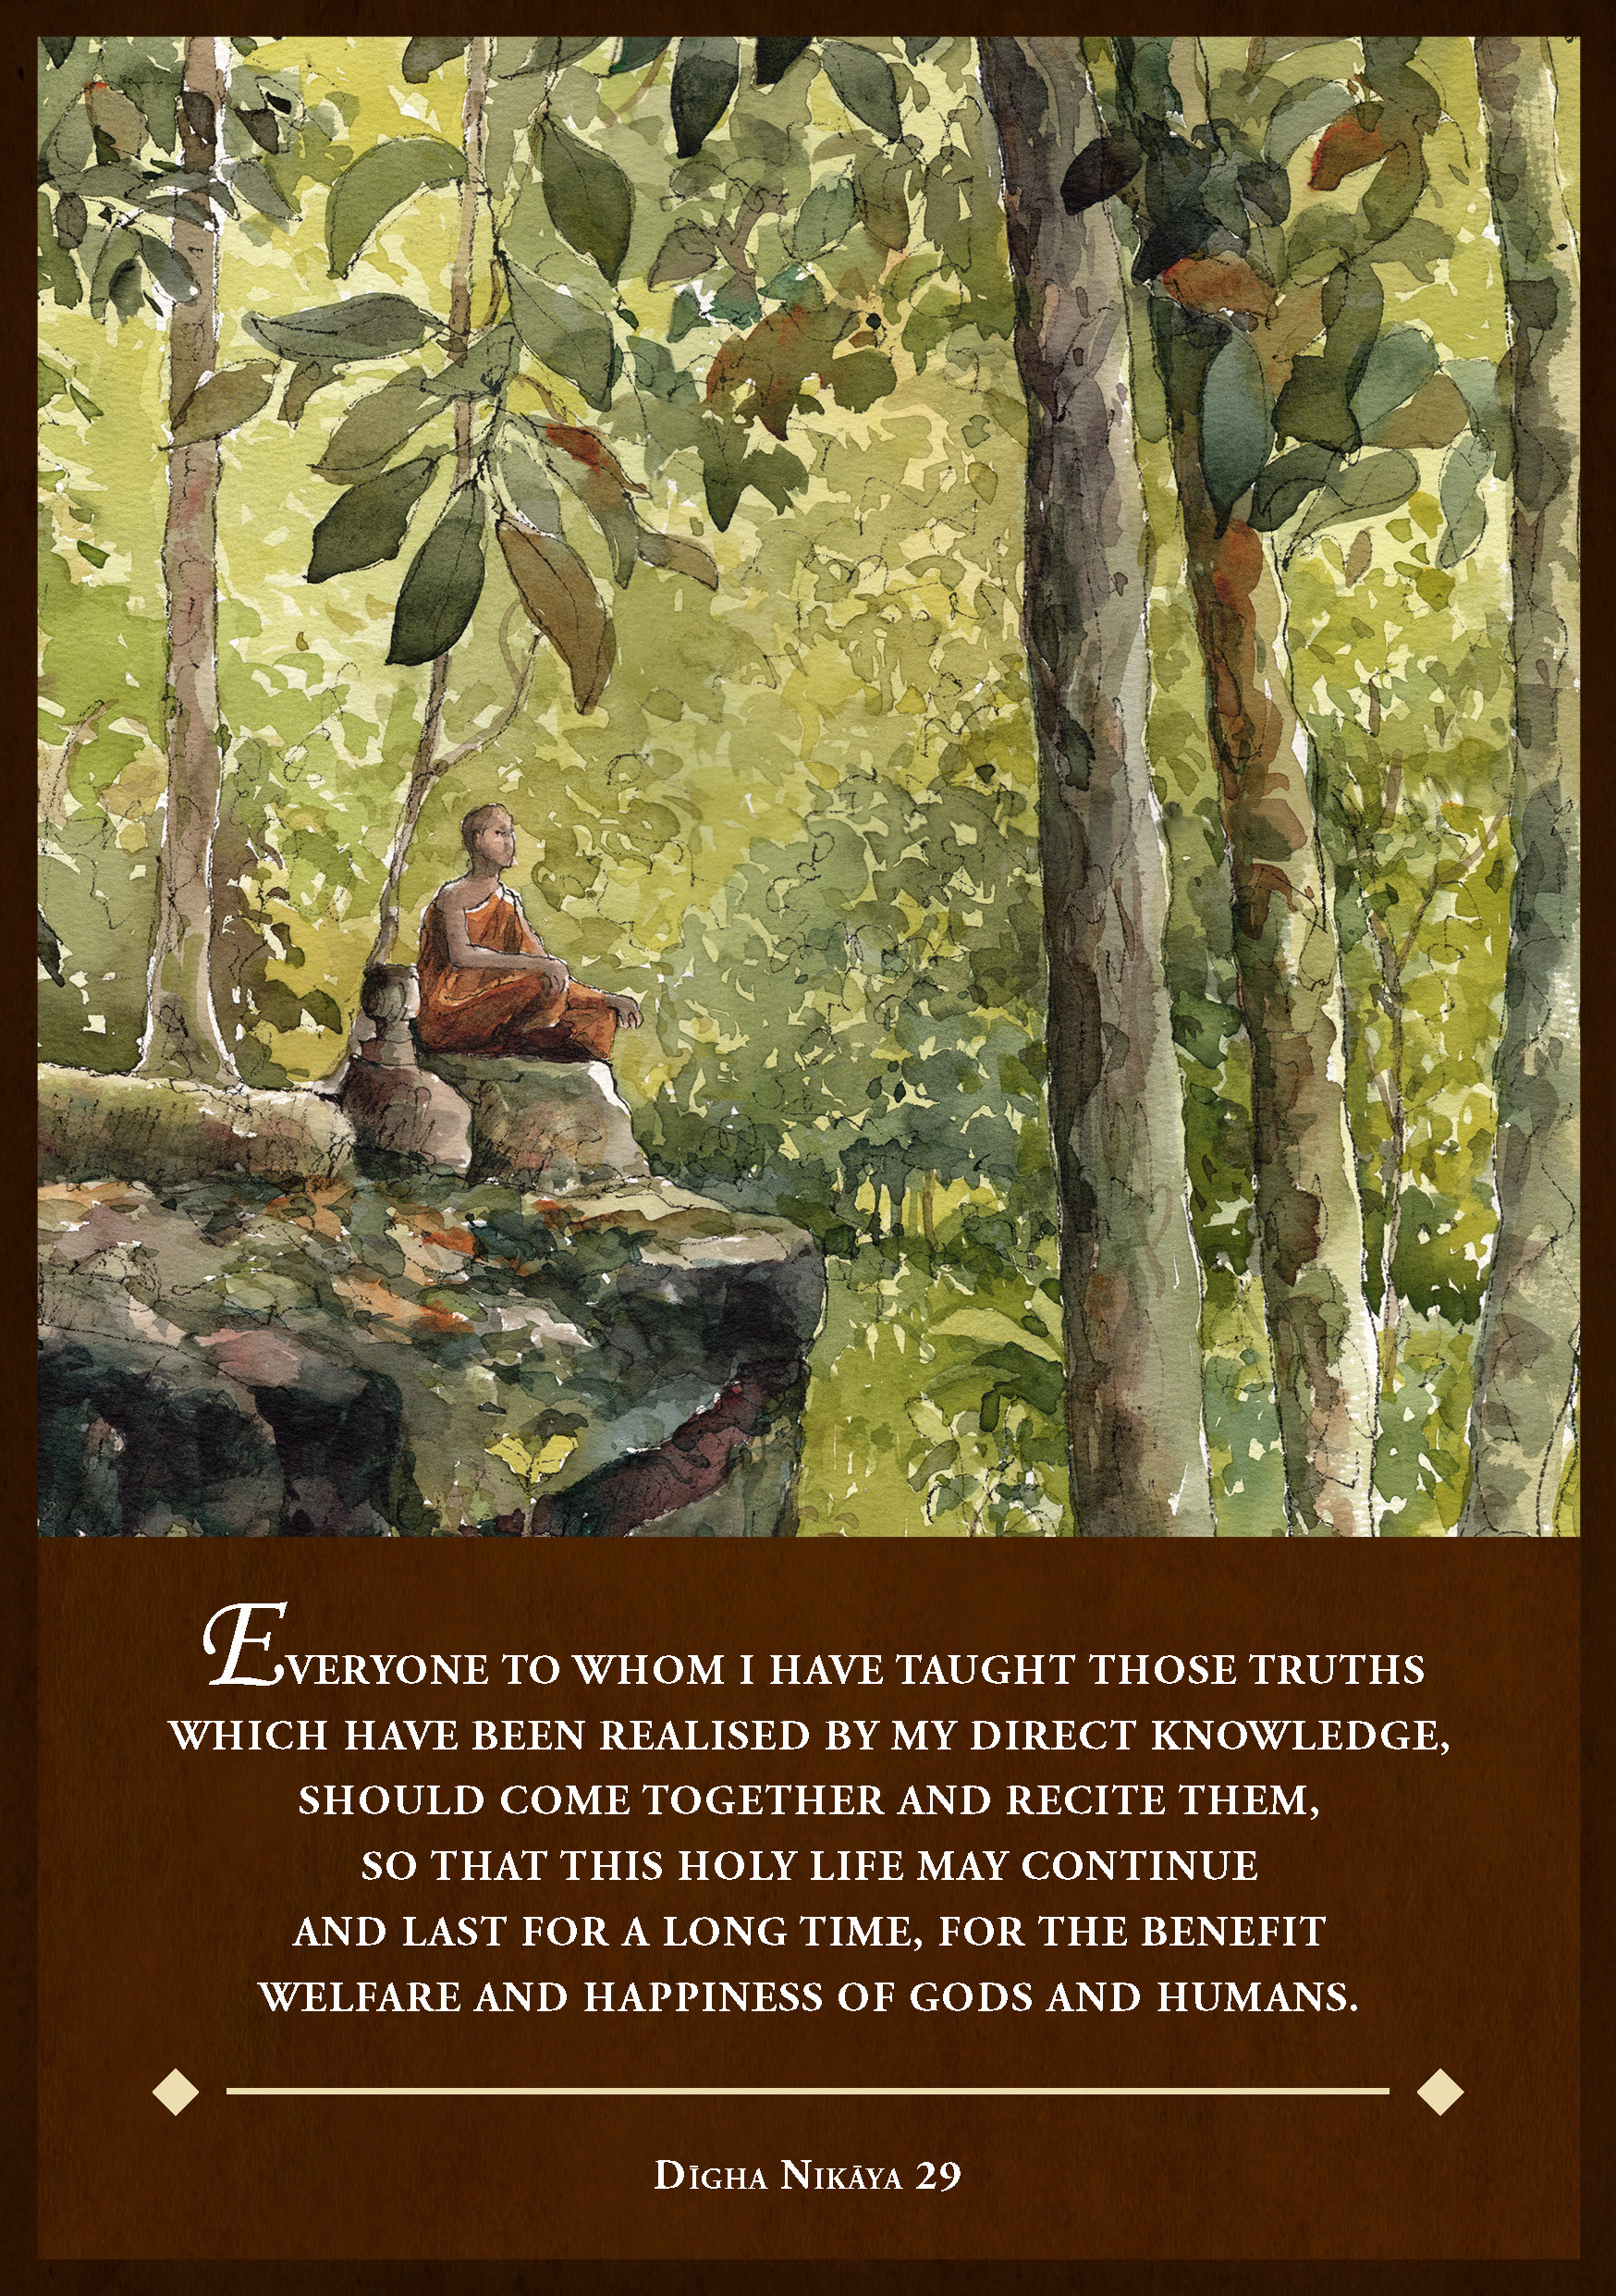
\includegraphics[height=\paperheight]{./assets/images/A5/back_cover_compressed_A5.jpg}}
\fi

\ifninebythirteenversion
  \photoFullBleed{./assets/images/9x13/back_cover_9x13.png}
\fi

\ifbfiveversion
  \photoFullBleed{./assets/images/B5/back_cover_B5.png}
\fi

\end{document}
'
% Possible VALUE:
%   - afiveVersion —  A5 formatted
%   - ninebythirteenVersion —  9x13cm custom formatted
%   - bfiveVersion —  B5 formatted
% \listfiles
\ifdefined\papersizeoption
\else
  \newcommand{\papersizeoption}{bfiveVersion}
\fi
\typeout{Set \protect\papersizeoption{} to \papersizeoption}

% Add hyperlinks and images, to be used with afiveVersion \papersizeoption
% Build command:
% '\newcommand{\papersizeoption}{afiveVersion}\newcommand{\isdigitalversion}{}% Set paper variant
% Build command '\newcommand{\papersizeoption}{VALUE}% Set paper variant
% Build command '\newcommand{\papersizeoption}{VALUE}\input{main.tex}'
% Possible VALUE:
%   - afiveVersion —  A5 formatted
%   - ninebythirteenVersion —  9x13cm custom formatted
%   - bfiveVersion —  B5 formatted
% \listfiles
\ifdefined\papersizeoption
\else
  \newcommand{\papersizeoption}{bfiveVersion}
\fi
\typeout{Set \protect\papersizeoption{} to \papersizeoption}

% Add hyperlinks and images, to be used with afiveVersion \papersizeoption
% Build command:
% '\newcommand{\papersizeoption}{afiveVersion}\newcommand{\isdigitalversion}{}\input{main.tex}'
\ifdefined\isdigitalversion
  \newcommand{\digitaloption}{digitalVersion}
\else
  \newcommand{\digitaloption}{}
\fi
\typeout{Set \protect\digitaloption{} to \digitaloption}

% todo ask bergen to make showtims a togglable condition for b5 and 9x13 only

\documentclass[
  final,
  babelLanguage=british,
  showtrims,
  \papersizeoption,
  \digitaloption,
]{anecdote}

% Define graphics path for images
\graphicspath{
  {./assets/images/A5}
  {./assets/images/9x13}
  {./assets/images/B5}
  {./assets/images/graphics}
}

% Loads formatting for selected ddocument class
\ifninebythirteenversion \usepackage{9x13} \fi
\ifafiveversion \usepackage{A5} \fi
\ifbfiveversion \usepackage{B5} \fi

% Set metadata for the document
\title{SBS Pāli-English Recitations}
\subtitle{Monk Training Centre}
\author{SBS Monk Training Centre}
\publisher{Sāsanārakkha Buddhist Sanctuary}
\date{2021-10-30}
\editionInfo{\textit{First Edition}, 2025} % And last edition. Don't call Pāladhammika.
\newcommand{\MyISBN}{} % default empty

\ifbfiveversion
  \renewcommand{\MyISBN}{978-629-97831-1-4}
\fi
\ifninebythirteenversion
  \renewcommand{\MyISBN}{978-629-97831-2-1}
\fi

\ISBN{\MyISBN}

% Set metadata for PDF properties
\hypersetup{
  pdftitle={\thetitle},
  pdfauthor={\theauthor},
  pdfcopyright={Copyright (C) 2025, \thePublisher},
  pdfsubject={},
  pdfkeywords={},
  pdflicenseurl={https://creativecommons.org/licenses/by-nc-nd/4.0/},
  pdfcontacturl={},
  pdflang={en},
}

% Load further packages
\RequirePackage[yyyymmdd,hhmmss]{datetime} % Adds the time to version creation

\makepagenote
\continuousnotenums % Ensure continuous endnote numbering

% Define hyphenation exceptions and corrections
\hyphenation{London re-lin-quishes de-ter-mines}

\ifdigitalversion
  \openany
\fi

% Begin document
\begin{document}

% Front matter
\frontmatter

% Digital version cover
\ifdigitalversion
	\digitalCover{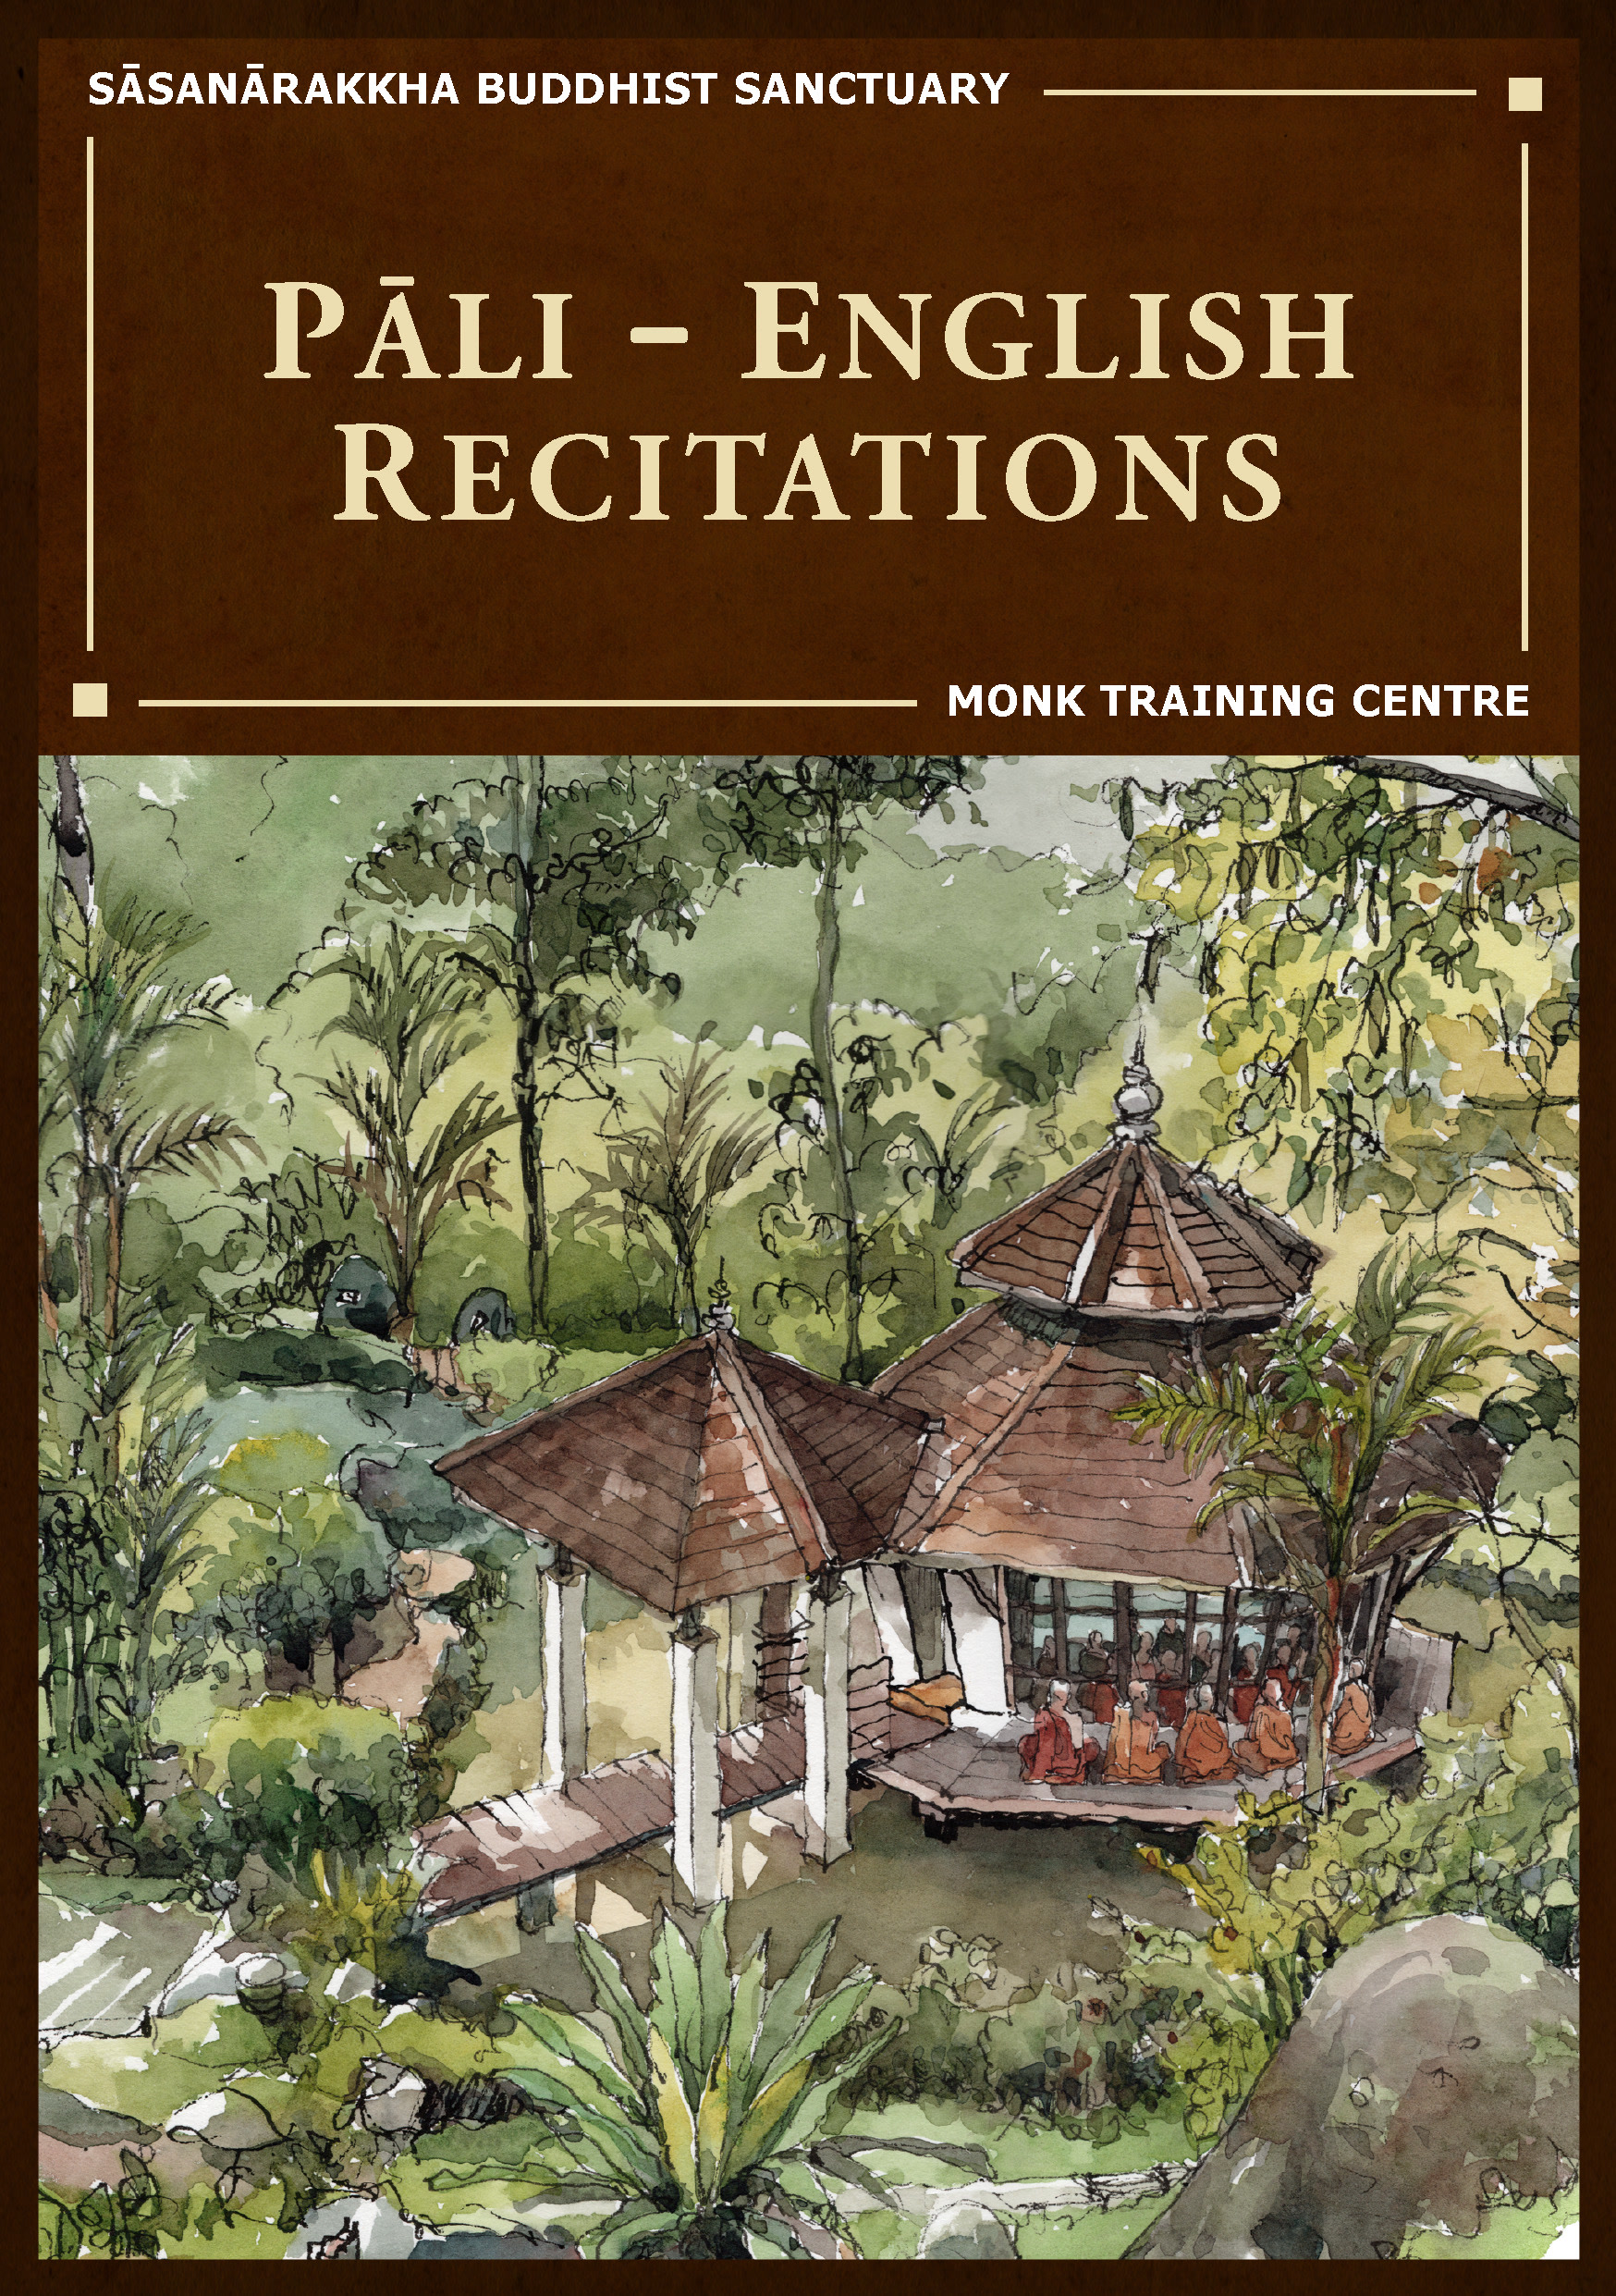
\includegraphics[height=\paperheight]{./assets/images/A5/front_cover_compressed_A5.jpg}}
\fi

\ifninebythirteenversion
  \photoFullBleed{./assets/images/9x13/front_cover_9x13.png}
  \photoFullBleed{robe_divider_left_9x13.png}
  \photoFullBleed{robe_divider_right_9x13.png}
\fi

\ifbfiveversion
  \photoFullBleed{./assets/images/B5/front_cover_B5.png}
  \photoFullBleed{robe_divider_left_B5.png}
  \photoFullBleed{robe_divider_right_B5.png}
\fi

% Title page, copyright, acknowledgments
\pagestyle{empty}
\input{./tex/titlepage.tex}
\input{./tex/copyright.tex}
\input{./tex/acknowledgments.tex}

% Table of contents, schedule, purpose and benefits, abbreviations
\cleartorecto
\pagestyle{toponerow-frontmatter}
\chapterstyle{adrasteia-toc}

\pdfbookmark[section]{\contentsname}{toc}
\tableofcontents*

\input{./tex/schedule.tex}
\input{./tex/purpose-and-benefits.tex}
\input{./tex/abbreviations.tex}

\chapterstyle{adrasteia-frontmatter}

% Main matter
\mainmatter
\pagestyle{toponerow}

\cleartorecto

% Chapters
{\raggedright
	\input{./tex/recitations/homage.tex}
	\input{./tex/recitations/verses.tex}
	\input{./tex/recitations/teachings.tex}
	\input{./tex/recitations/reflections.tex}
	\input{./tex/recitations/cardinal-discourses.tex}
	\input{./tex/recitations/thanksgiving-recitations.tex}
	\input{./tex/recitations/protective-recitations.tex}
	\input{./tex/recitations/funeral-recitations.tex}
	\input{./tex/recitations/sharing-of-merits.tex}
}

% Appendix
\appendix
\input{./tex/appendix.tex}
\input{./tex/refuge-trainings.tex}
\input{./tex/phonetics-pronunciation.tex}
\input{./tex/guidelines.tex}

% Back matter
\backmatter
\printpagenotes % Print endnotes
\input{./tex/copyright-details.tex}

\ifbfiveversion
  \includepdf[pages=-,pagecommand={\thispagestyle{empty}}]{assets/images/graphics/donor-list.pdf}
  \photoFullBleed{robe_divider_left_B5.png}
  \photoFullBleed{robe_divider_right_B5.png}
\fi

\ifninebythirteenversion
  \photoFullBleed{robe_divider_left_9x13.png}
  \photoFullBleed{robe_divider_right_9x13.png}
\fi

\emptyUntilEven % Add blank page if necessary

\ifdigitalversion
  \clearpage
  \digitalCover{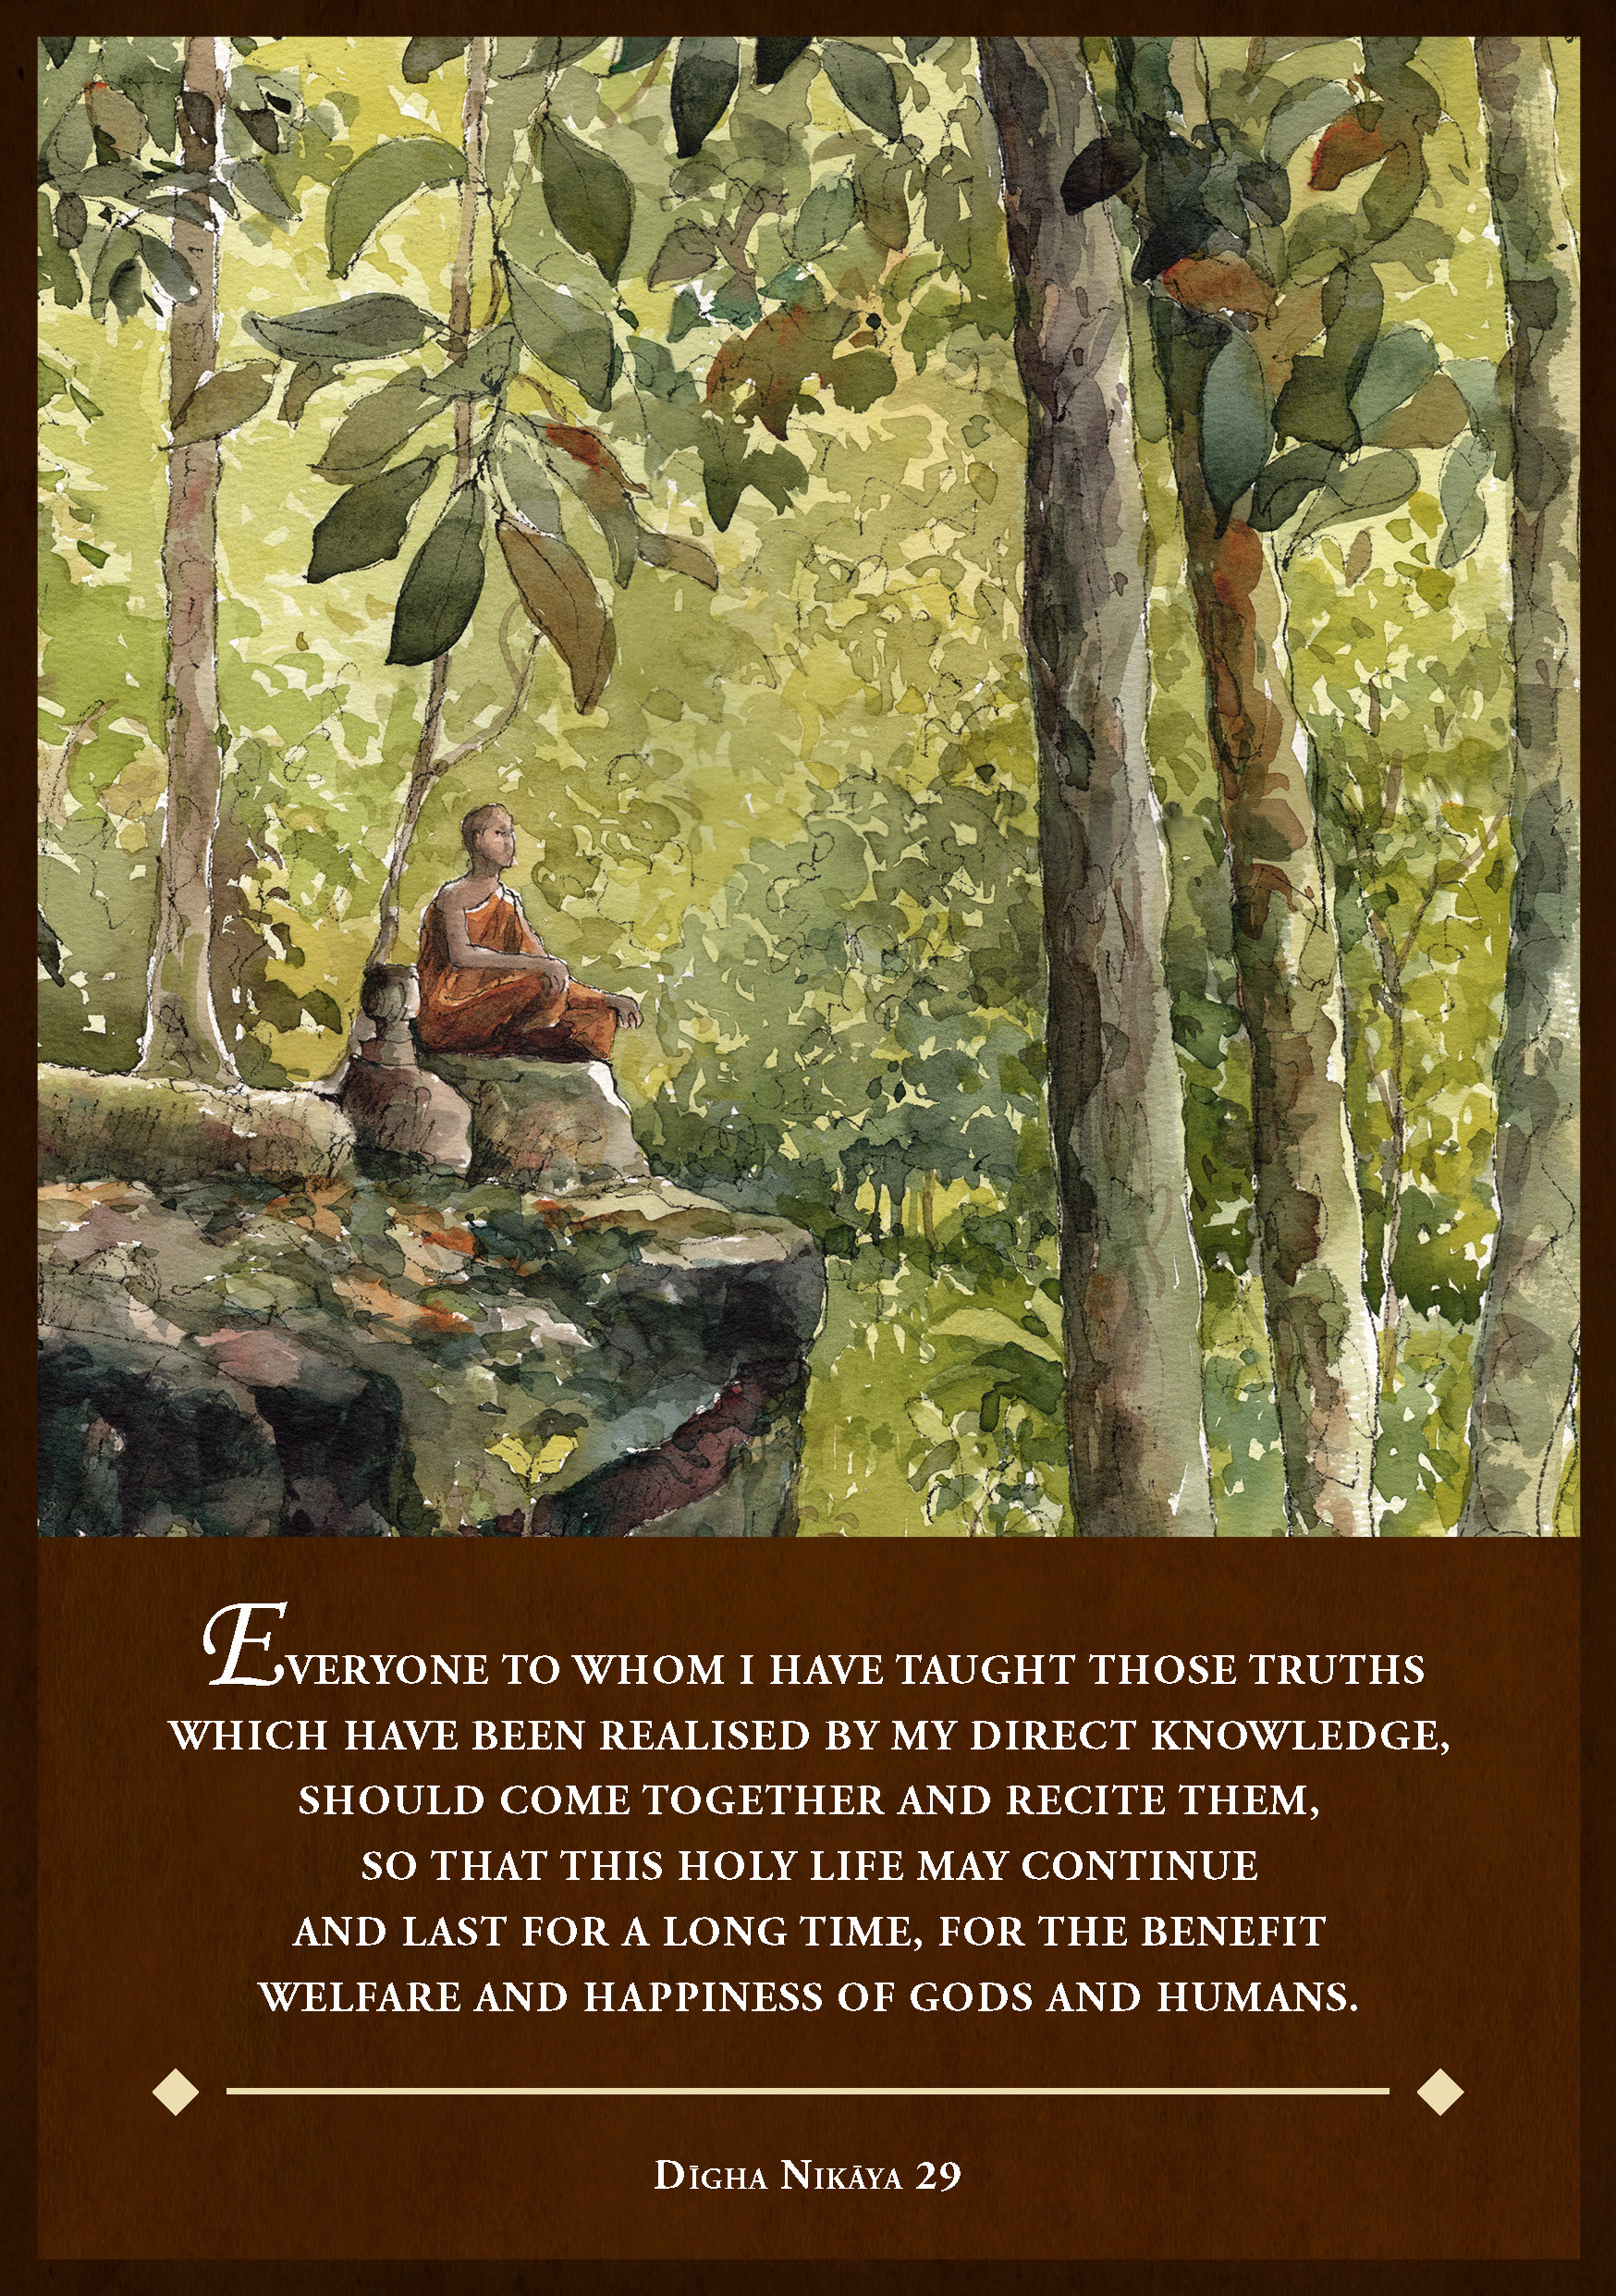
\includegraphics[height=\paperheight]{./assets/images/A5/back_cover_compressed_A5.jpg}}
\fi

\ifninebythirteenversion
  \photoFullBleed{./assets/images/9x13/back_cover_9x13.png}
\fi

\ifbfiveversion
  \photoFullBleed{./assets/images/B5/back_cover_B5.png}
\fi

\end{document}
'
% Possible VALUE:
%   - afiveVersion —  A5 formatted
%   - ninebythirteenVersion —  9x13cm custom formatted
%   - bfiveVersion —  B5 formatted
% \listfiles
\ifdefined\papersizeoption
\else
  \newcommand{\papersizeoption}{bfiveVersion}
\fi
\typeout{Set \protect\papersizeoption{} to \papersizeoption}

% Add hyperlinks and images, to be used with afiveVersion \papersizeoption
% Build command:
% '\newcommand{\papersizeoption}{afiveVersion}\newcommand{\isdigitalversion}{}% Set paper variant
% Build command '\newcommand{\papersizeoption}{VALUE}\input{main.tex}'
% Possible VALUE:
%   - afiveVersion —  A5 formatted
%   - ninebythirteenVersion —  9x13cm custom formatted
%   - bfiveVersion —  B5 formatted
% \listfiles
\ifdefined\papersizeoption
\else
  \newcommand{\papersizeoption}{bfiveVersion}
\fi
\typeout{Set \protect\papersizeoption{} to \papersizeoption}

% Add hyperlinks and images, to be used with afiveVersion \papersizeoption
% Build command:
% '\newcommand{\papersizeoption}{afiveVersion}\newcommand{\isdigitalversion}{}\input{main.tex}'
\ifdefined\isdigitalversion
  \newcommand{\digitaloption}{digitalVersion}
\else
  \newcommand{\digitaloption}{}
\fi
\typeout{Set \protect\digitaloption{} to \digitaloption}

% todo ask bergen to make showtims a togglable condition for b5 and 9x13 only

\documentclass[
  final,
  babelLanguage=british,
  showtrims,
  \papersizeoption,
  \digitaloption,
]{anecdote}

% Define graphics path for images
\graphicspath{
  {./assets/images/A5}
  {./assets/images/9x13}
  {./assets/images/B5}
  {./assets/images/graphics}
}

% Loads formatting for selected ddocument class
\ifninebythirteenversion \usepackage{9x13} \fi
\ifafiveversion \usepackage{A5} \fi
\ifbfiveversion \usepackage{B5} \fi

% Set metadata for the document
\title{SBS Pāli-English Recitations}
\subtitle{Monk Training Centre}
\author{SBS Monk Training Centre}
\publisher{Sāsanārakkha Buddhist Sanctuary}
\date{2021-10-30}
\editionInfo{\textit{First Edition}, 2025} % And last edition. Don't call Pāladhammika.
\newcommand{\MyISBN}{} % default empty

\ifbfiveversion
  \renewcommand{\MyISBN}{978-629-97831-1-4}
\fi
\ifninebythirteenversion
  \renewcommand{\MyISBN}{978-629-97831-2-1}
\fi

\ISBN{\MyISBN}

% Set metadata for PDF properties
\hypersetup{
  pdftitle={\thetitle},
  pdfauthor={\theauthor},
  pdfcopyright={Copyright (C) 2025, \thePublisher},
  pdfsubject={},
  pdfkeywords={},
  pdflicenseurl={https://creativecommons.org/licenses/by-nc-nd/4.0/},
  pdfcontacturl={},
  pdflang={en},
}

% Load further packages
\RequirePackage[yyyymmdd,hhmmss]{datetime} % Adds the time to version creation

\makepagenote
\continuousnotenums % Ensure continuous endnote numbering

% Define hyphenation exceptions and corrections
\hyphenation{London re-lin-quishes de-ter-mines}

\ifdigitalversion
  \openany
\fi

% Begin document
\begin{document}

% Front matter
\frontmatter

% Digital version cover
\ifdigitalversion
	\digitalCover{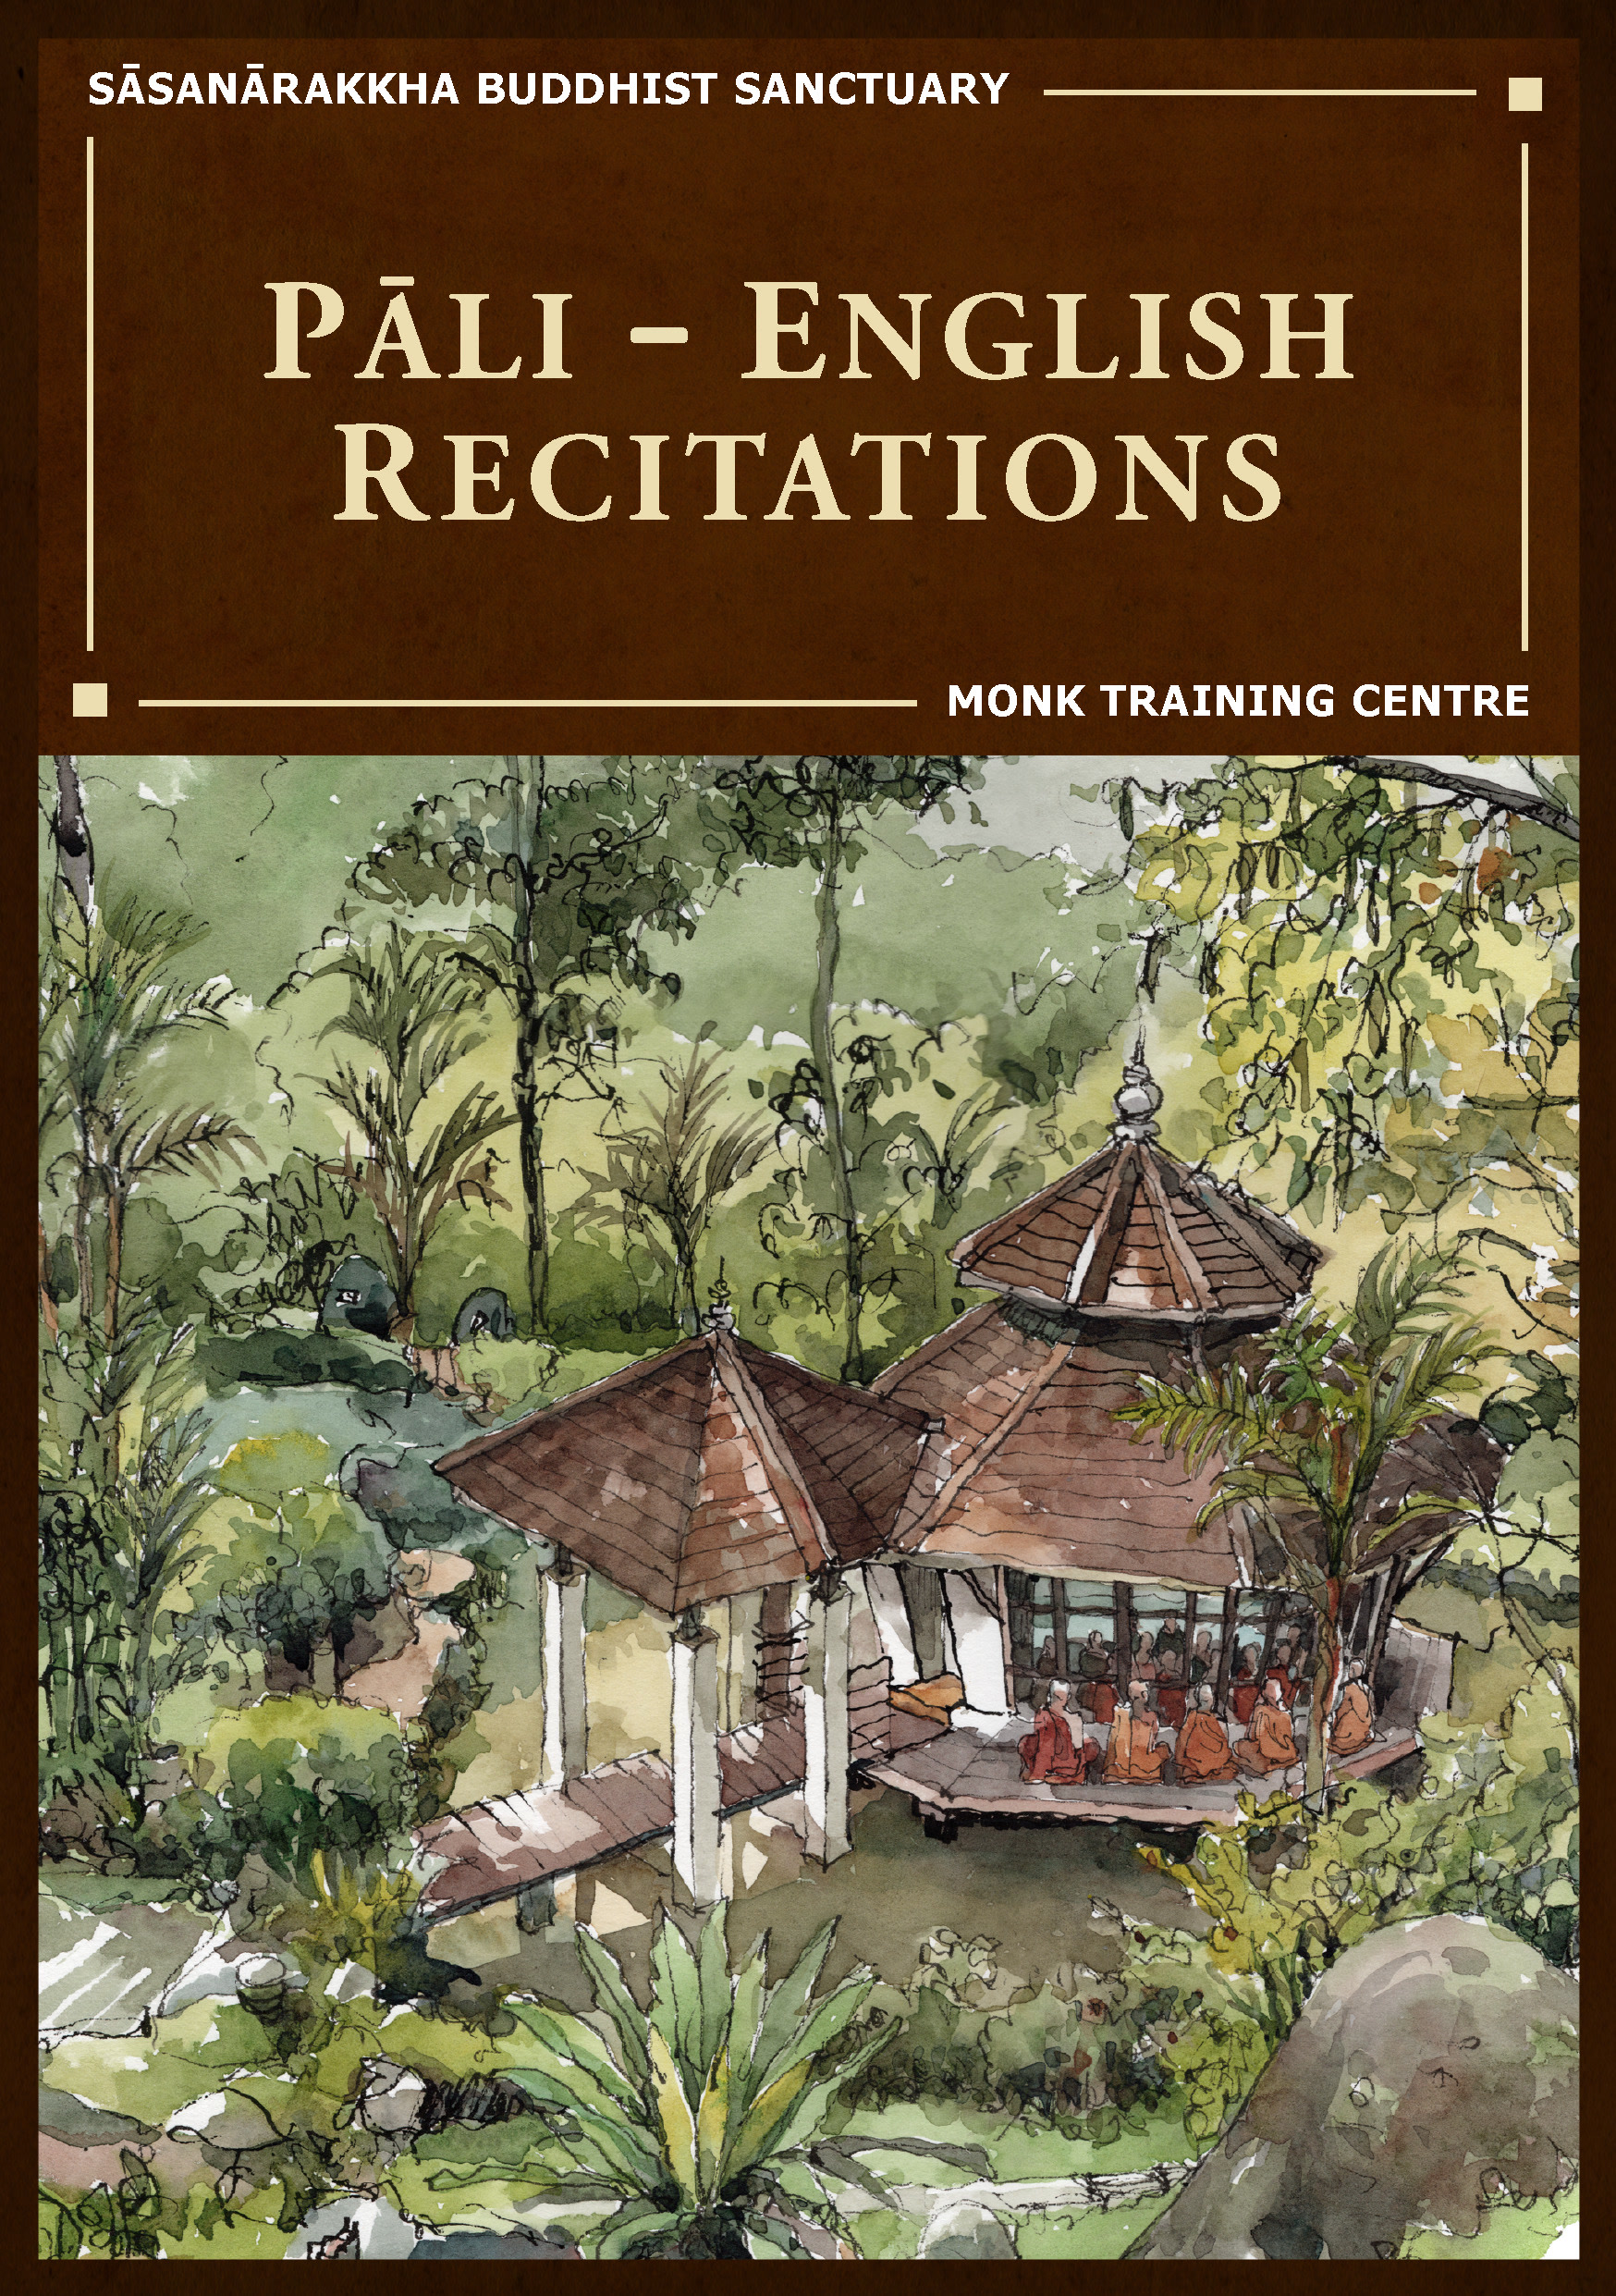
\includegraphics[height=\paperheight]{./assets/images/A5/front_cover_compressed_A5.jpg}}
\fi

\ifninebythirteenversion
  \photoFullBleed{./assets/images/9x13/front_cover_9x13.png}
  \photoFullBleed{robe_divider_left_9x13.png}
  \photoFullBleed{robe_divider_right_9x13.png}
\fi

\ifbfiveversion
  \photoFullBleed{./assets/images/B5/front_cover_B5.png}
  \photoFullBleed{robe_divider_left_B5.png}
  \photoFullBleed{robe_divider_right_B5.png}
\fi

% Title page, copyright, acknowledgments
\pagestyle{empty}
\input{./tex/titlepage.tex}
\input{./tex/copyright.tex}
\input{./tex/acknowledgments.tex}

% Table of contents, schedule, purpose and benefits, abbreviations
\cleartorecto
\pagestyle{toponerow-frontmatter}
\chapterstyle{adrasteia-toc}

\pdfbookmark[section]{\contentsname}{toc}
\tableofcontents*

\input{./tex/schedule.tex}
\input{./tex/purpose-and-benefits.tex}
\input{./tex/abbreviations.tex}

\chapterstyle{adrasteia-frontmatter}

% Main matter
\mainmatter
\pagestyle{toponerow}

\cleartorecto

% Chapters
{\raggedright
	\input{./tex/recitations/homage.tex}
	\input{./tex/recitations/verses.tex}
	\input{./tex/recitations/teachings.tex}
	\input{./tex/recitations/reflections.tex}
	\input{./tex/recitations/cardinal-discourses.tex}
	\input{./tex/recitations/thanksgiving-recitations.tex}
	\input{./tex/recitations/protective-recitations.tex}
	\input{./tex/recitations/funeral-recitations.tex}
	\input{./tex/recitations/sharing-of-merits.tex}
}

% Appendix
\appendix
\input{./tex/appendix.tex}
\input{./tex/refuge-trainings.tex}
\input{./tex/phonetics-pronunciation.tex}
\input{./tex/guidelines.tex}

% Back matter
\backmatter
\printpagenotes % Print endnotes
\input{./tex/copyright-details.tex}

\ifbfiveversion
  \includepdf[pages=-,pagecommand={\thispagestyle{empty}}]{assets/images/graphics/donor-list.pdf}
  \photoFullBleed{robe_divider_left_B5.png}
  \photoFullBleed{robe_divider_right_B5.png}
\fi

\ifninebythirteenversion
  \photoFullBleed{robe_divider_left_9x13.png}
  \photoFullBleed{robe_divider_right_9x13.png}
\fi

\emptyUntilEven % Add blank page if necessary

\ifdigitalversion
  \clearpage
  \digitalCover{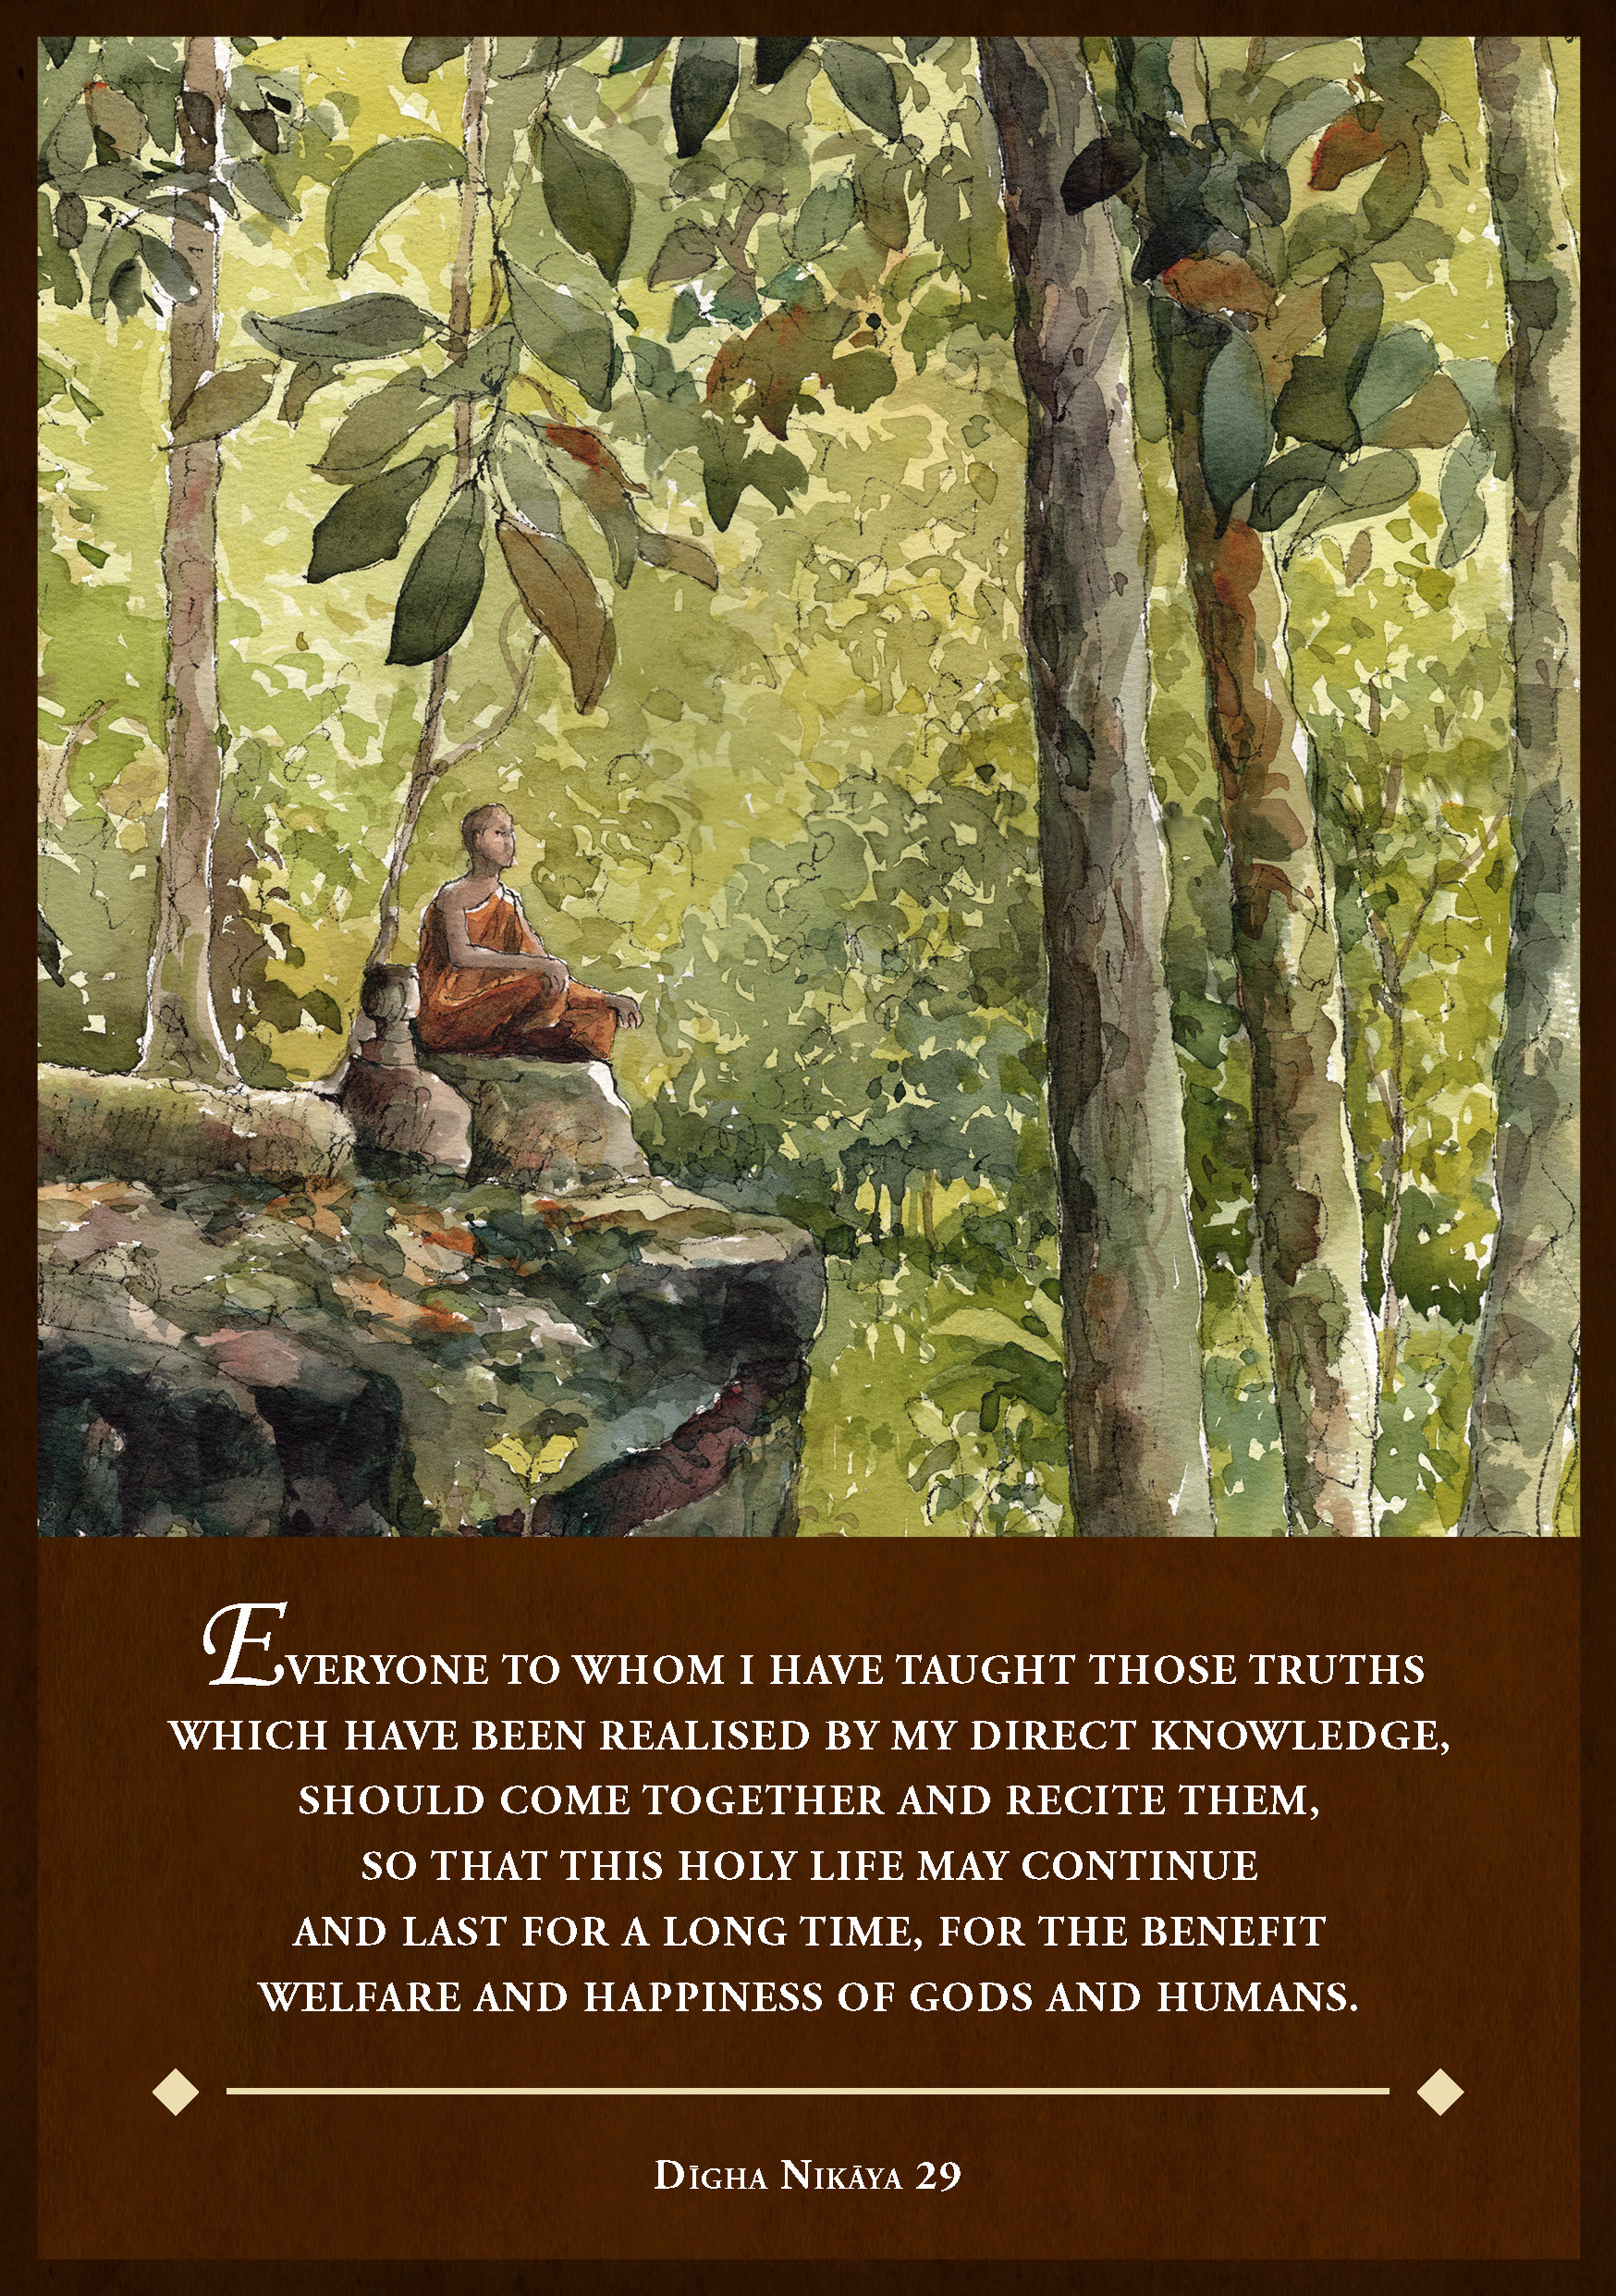
\includegraphics[height=\paperheight]{./assets/images/A5/back_cover_compressed_A5.jpg}}
\fi

\ifninebythirteenversion
  \photoFullBleed{./assets/images/9x13/back_cover_9x13.png}
\fi

\ifbfiveversion
  \photoFullBleed{./assets/images/B5/back_cover_B5.png}
\fi

\end{document}
'
\ifdefined\isdigitalversion
  \newcommand{\digitaloption}{digitalVersion}
\else
  \newcommand{\digitaloption}{}
\fi
\typeout{Set \protect\digitaloption{} to \digitaloption}

% todo ask bergen to make showtims a togglable condition for b5 and 9x13 only

\documentclass[
  final,
  babelLanguage=british,
  showtrims,
  \papersizeoption,
  \digitaloption,
]{anecdote}

% Define graphics path for images
\graphicspath{
  {./assets/images/A5}
  {./assets/images/9x13}
  {./assets/images/B5}
  {./assets/images/graphics}
}

% Loads formatting for selected ddocument class
\ifninebythirteenversion \usepackage{9x13} \fi
\ifafiveversion \usepackage{A5} \fi
\ifbfiveversion \usepackage{B5} \fi

% Set metadata for the document
\title{SBS Pāli-English Recitations}
\subtitle{Monk Training Centre}
\author{SBS Monk Training Centre}
\publisher{Sāsanārakkha Buddhist Sanctuary}
\date{2021-10-30}
\editionInfo{\textit{First Edition}, 2025} % And last edition. Don't call Pāladhammika.
\newcommand{\MyISBN}{} % default empty

\ifbfiveversion
  \renewcommand{\MyISBN}{978-629-97831-1-4}
\fi
\ifninebythirteenversion
  \renewcommand{\MyISBN}{978-629-97831-2-1}
\fi

\ISBN{\MyISBN}

% Set metadata for PDF properties
\hypersetup{
  pdftitle={\thetitle},
  pdfauthor={\theauthor},
  pdfcopyright={Copyright (C) 2025, \thePublisher},
  pdfsubject={},
  pdfkeywords={},
  pdflicenseurl={https://creativecommons.org/licenses/by-nc-nd/4.0/},
  pdfcontacturl={},
  pdflang={en},
}

% Load further packages
\RequirePackage[yyyymmdd,hhmmss]{datetime} % Adds the time to version creation

\makepagenote
\continuousnotenums % Ensure continuous endnote numbering

% Define hyphenation exceptions and corrections
\hyphenation{London re-lin-quishes de-ter-mines}

\ifdigitalversion
  \openany
\fi

% Begin document
\begin{document}

% Front matter
\frontmatter

% Digital version cover
\ifdigitalversion
	\digitalCover{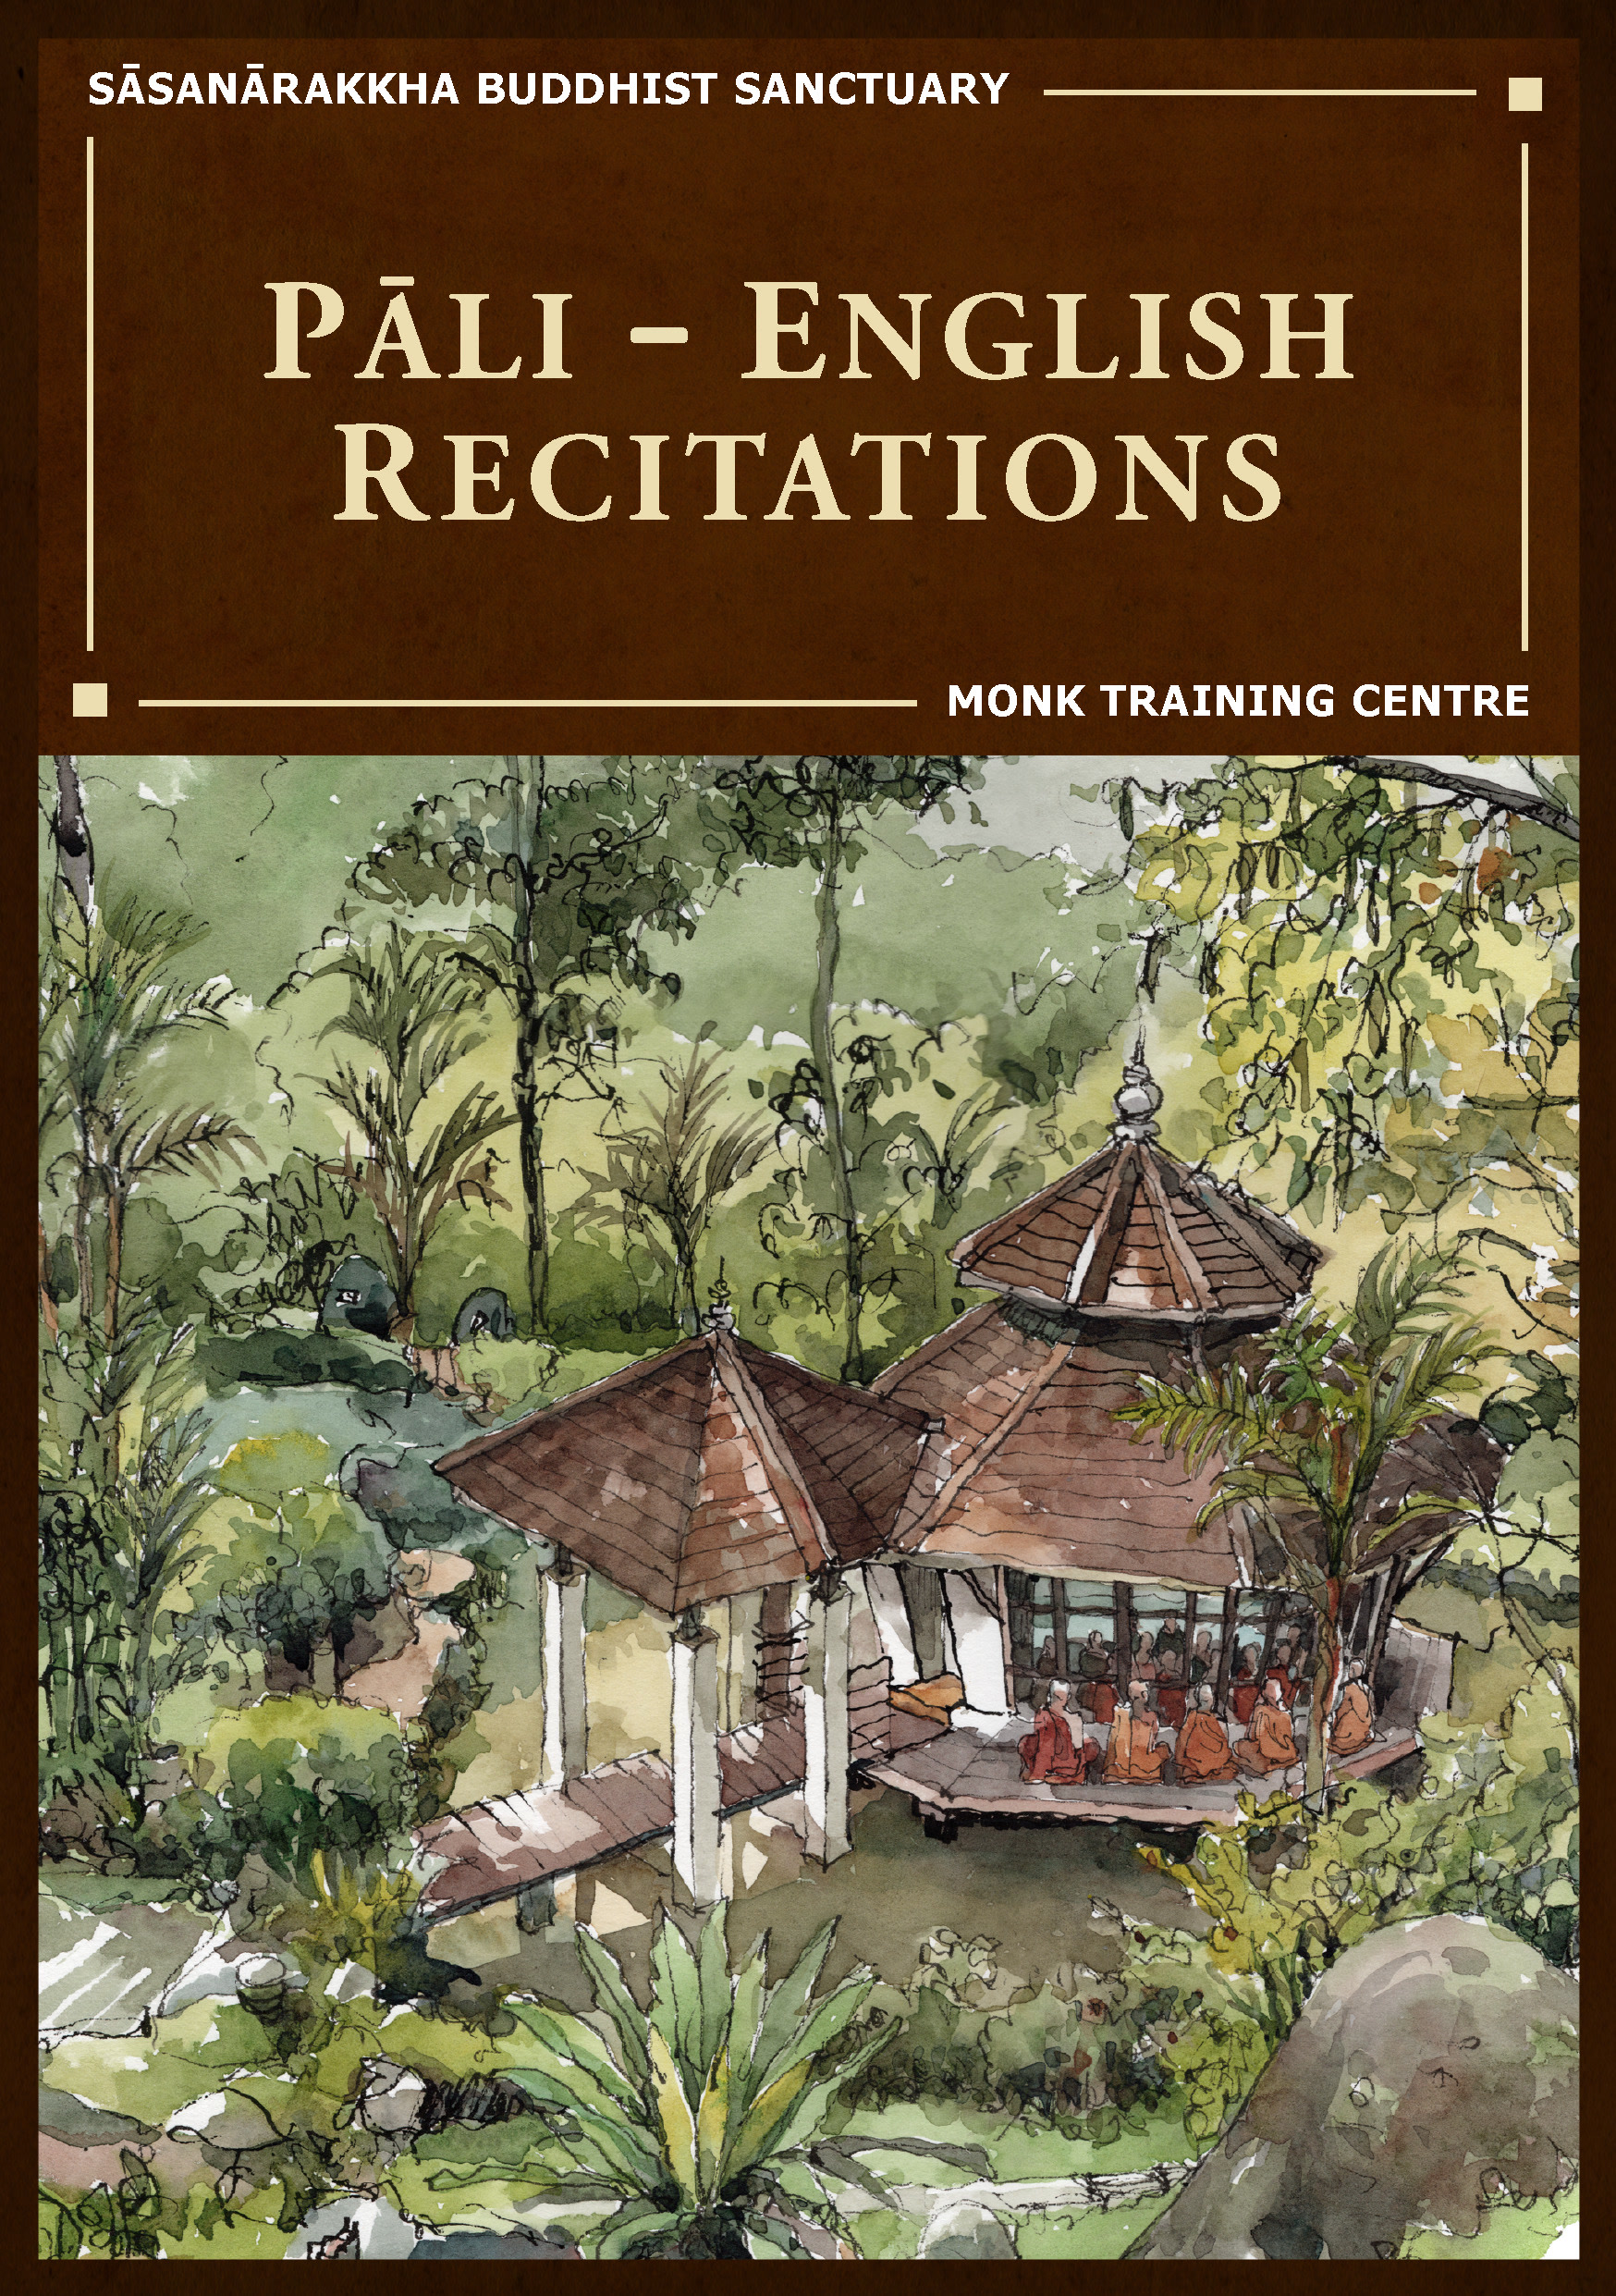
\includegraphics[height=\paperheight]{./assets/images/A5/front_cover_compressed_A5.jpg}}
\fi

\ifninebythirteenversion
  \photoFullBleed{./assets/images/9x13/front_cover_9x13.png}
  \photoFullBleed{robe_divider_left_9x13.png}
  \photoFullBleed{robe_divider_right_9x13.png}
\fi

\ifbfiveversion
  \photoFullBleed{./assets/images/B5/front_cover_B5.png}
  \photoFullBleed{robe_divider_left_B5.png}
  \photoFullBleed{robe_divider_right_B5.png}
\fi

% Title page, copyright, acknowledgments
\pagestyle{empty}

\cleartorecto
\thispagestyle{empty}

\vspace*{3em}

{\centering

  \settowidth{\titleLength}{%
    {\Large\chapterTitleFont\textsc{\MakeUppercase{{Pāli-English Recitations}}}}%
  }

  % 'SBS' on title page
  \ifafive {\Huge\fontsize{64}{16}\sbsFont SBS}\\[1.0\baselineskip] \fi
  \ifninebythirteen {\Huge\fontsize{42.5}{11}\sbsFont SBS}\\[1.0\baselineskip] \fi
  \ifbfive {\Huge\fontsize{80}{16}\sbsFont SBS}\\[1.0\baselineskip] \fi

  % 'Monk Training Centre'
  \ifafive \setlength{\xheight}{\heightof{X}}
    {\Huge\chapterTitleFont\textsc{{\thesubtitle\linebreak}}}\\[0.2\baselineskip] \fi
  \ifninebythirteen {\fontsize{16}{14}\chapterTitleFont\textsc{{\thesubtitle\linebreak}}}\\[0.2\baselineskip] \fi
  \ifbfive \setlength{\xheight}{\heightof{X}}
    {\fontsize{30}{14}\chapterTitleFont\textsc{{\thesubtitle\linebreak}}}\\[0.2\baselineskip] \fi

  % Ornament
  \ifafive \raisebox{0.5\xheight}{\pgfornament[color=sbs-brown,width=7cm,scale=1,ydelta=0pt,symmetry=c]{84}}\\[1.4\baselineskip] \fi
  \ifninebythirteen \raisebox{0.5\xheight}{\pgfornament[color=sbs-brown,width=4.5cm,scale=1,ydelta=0pt,symmetry=c]{84}}\\[1.4\baselineskip] \fi
  \ifbfive \raisebox{0.5\xheight}{\pgfornament[color=sbs-brown,width=8.5cm,scale=1,ydelta=0pt,symmetry=c]{84}}\\[1.4\baselineskip] \fi


  % 'Pali-English Recitations'
  \ifafive {\Large\scshape Pāli-English Recitations}\\[2.5\baselineskip] \fi
  \ifninebythirteen {\fontsize{10}{12}\scshape Pāli-English Recitations}\\[2.5\baselineskip] \fi
  \ifbfive {\fontsize{18.5}{12}\scshape Pāli-English Recitations}\\[2.5\baselineskip] \fi

  % Dhamma quote
  {\quote ``In whatever way a bhikkhu recites the Dhamma in detail as he has heard it and learned it, in just that way, in relation to that Dhamma, he experiences inspiration in the meaning and inspiration in the Dhamma. As he does so, joy arises in him. When he is joyful, rapture arises. For one with a rapturous mind, the body becomes tranquil. One tranquil in body feels pleasure. For one feeling pleasure, the mind becomes concentrated.''\\}
  \ifafive \smallskip AN 5.26\\[1.4\baselineskip]\fi
  \ifninebythirteen \smallskip \fontsize{8}{14}\selectfont AN 5.26\\[1.4\baselineskip]\fi
  %% \ifbfive \smallskip \fontsize{8.5}{14}\selectfont AN 5.26\\[1.4\baselineskip]\fi
  \ifbfive \smallskip AN 5.26\\[1.4\baselineskip]\fi
}



\cleartoverso
\thispagestyle{empty}

{%

  \ifafive \fontsize{10}{16}\selectfont \fi
  \ifninebythirteen \fontsize{7.5}{11}\selectfont \fi
  \ifbfive \fontsize{12}{20}\selectfont \fi
  \centering
  \setlength{\parindent}{0pt}%

  \ifafive \vspace{0.5cm} \fi
  \ifninebythirteen \vspace{0.4cm} \fi
  \ifbfive \vspace{0.5cm} \fi

  \copyright\ \thePublisher, 2025\\
  c/o 160, Lorong 3, Jalan Merdeka, 34000 Taiping, Perak, Malaysia\\
  \ifdigital
    \else
  ISBN \theISBN
  \fi

  \ifafive \vspace{0.5cm} \fi
  \ifninebythirteen \vspace{0.3cm} \fi
  \ifbfive \vspace{0.5cm} \fi

  This book is for free distribution only;\\
  it may not be sold.

  \ifafive \vspace{0.5cm} \fi
  \ifninebythirteen \vspace{0.3cm} \fi
  \ifbfive \vspace{0.5cm} \fi

  Download this book as a PDF, EPUB, MOBI, AZW3\\
  at the following address:\\
  \href{https://sasanarakkha.org/recitations}{https://sasanarakkha.org/recitations}

Accompanying audio recordings can be found at:
\href{https://www.youtube.com/SasanarakkhaBuddhistSanctuary}{https://www.youtube.com/SasanarakkhaBuddhistSanctuary}

  \ifafive \vspace{0.5cm} \fi
  \ifninebythirteen \vspace{0.3cm} \fi
  \ifbfive \vspace{0.5cm} \fi

  Project Manager: Ā. Ariyadhammika\\
  Editor: Ā. Pāladhammika\\
  Typesetting: Aj. Gambhiro, Ā. Pāladhammika\\
  Translators: Ā. Aggacitta, Ā. Bodhi, Aj. Kevalī, Ā. Sujāto, M. Walshe\\
  Endnotes: Ā. Ariyadhammika\\
  Watercolor Paintings: Lim Jee Yuan

  \ifafive \vspace{0.5cm} \fi
  \ifninebythirteen \vspace{0.3cm} \fi
  \ifbfive \vspace{0.5cm} \fi

  This work is licensed under a Creative Commons\\
  Attribution-NonCommercial-NoDerivatives 4.0 International~License.

  % Produced with the \LaTeX\ typesetting system,\\
  % set in Libertinus Serif.

  \ifafive  \vspace{0.5cm} \fi
  \ifninebythirteen \vspace{0.3cm} \fi
  \ifbfive \vspace{0.5cm} \fi

  \ifdigital
    This version was created on:\\
    \today \space at \currenttime\\
  \fi

  \ifafive \vspace{0.5cm} \fi
  \ifninebythirteen \vspace{0.15cm} \fi
  \ifbfive \vspace{0.5cm} \fi

  \theEditionInfo

}

\ifdigital

\else

\clearpage

\fi



\cleartorecto
\thispagestyle{empty}

{

  \setlength{\parskip}{10pt}

  \ifafive {\centering\fontsize{16}{25}\selectfont \textsc{We Wish To Gratefully Acknowledge} \par} \fi
  \ifninebythirteen {\centering\fontsize{10}{18}\selectfont \textsc{We Wish To Gratefully Acknowledge} \par} \fi
  \ifbfive {\centering\fontsize{18.5}{25}\selectfont \textsc{We Wish To Gratefully Acknowledge} \par} \fi


  The Saṅghas of Wat Pah Nanachat (WPN), Amaravati, and Abhayagiri for allowing the use of material from their respective chanting books, the late Ven. Dr. Saddhātissa and Mr. Maurice Walshe for their English translations, as well as Ven. Bhikkhu Bodhi for granting permission to use and slightly adapt his translations. Various Saṅgha members of SBS Monk Training Centre, who contributed in the compilation of an interesting selection of chants, as well as for providing countless suggestions to help improve the English translations.

  \linkdest{endnote1-body}
  Additional information on translations, as well as deviations\makeatletter\hyperlink{endnote1-appendix}\Hy@raisedlink{{\pagenote{%
        \hypertarget{endnote1-appendix}{\hyperlink{endnote1-body}{Due to the balanced and inspiring selection of chants, as well as for the sake of compatibility, WPN’s \textit{Buddhist Chanting} (2014) has served as the basis for this book. Over time, suggestions for the inclusion of additional chants, as well as occasional improvements of existing translations were incorporated. Such changes were meticulously marked down in the endnotes of the digital versions of this chanting book, so that someone familiar with the present book can straight away find the relevant differences, which can be useful when visiting a branch monastery of the Ajahn Chah lineage, in order to know in which places to revert to the original version.}}}}}\makeatother\thickspace
  from WPN's \textit{Buddhist Chanting} (2014), have been annotated by Ven. Ariyadhammika in the endnotes.


  \ifninebythirteen \smallskip \else \medskip \fi

  {\centering

    To Āyasmā Aggacitta, the founding father of\\
    Sāsanārakkha Buddhist Sanctuary.

    % \ifninebythirteen \smallskip \else \medskip \fi

    \begin{center}
      \ifafive 
\includegraphics[height=54mm]{sbs_logo_tuck_loon_brown.jpg} \fi
      \ifninebythirteen \clearpage \vspace*{\fill}
 
\includegraphics[height=80mm]{sbs_logo_tuck_loon_brown.jpg} \vspace*{\fill} \fi
      \ifbfive \vspace{1cm} 
\includegraphics[height=70mm]{sbs_logo_tuck_loon_brown.jpg}\fi
    \end{center}
  }
}



% Table of contents, schedule, purpose and benefits, abbreviations
\cleartorecto
\pagestyle{toponerow-frontmatter}
\chapterstyle{adrasteia-toc}

\pdfbookmark[section]{\contentsname}{toc}
\tableofcontents*


\chapter{Recitation Schedule}
\label{schedule}

{\centering

  {\pdfbookmark[2]{Set 1}{set1}\libertinusFont\selectfont\textbf{\textsc{\ifafive\fontsize{18}{12}\fi\ifninebythirteen\fontsize{13}{8.5}\fi\ifbfive\fontsize{22}{18}\fi\selectfont\textls*{Set 1}}}}\\
  \textsc{\ifafive\fontsize{14.4}{28}\fi\ifninebythirteen\fontsize{8.7}{17}\fi\ifbfive\fontsize{16}{33.5}\fi\selectfont
    \hyperref[buddhas-first-exclamation]{The Buddha's First Exclamation} \ifdigital\else\pageref{buddhas-first-exclamation}\fi\\
    \hyperref[wheel-of-dhamma-abridged]{Turning the Wheel of Dhamma} \ifdigital\else\pageref{wheel-of-dhamma-abridged}\fi\\
    \hyperref[true-false-refuges]{Going to True and False Refuges} \ifdigital\else\pageref{true-false-refuges}\fi\\
    \hyperref[four-great-references]{The Four Great References} \ifdigital\else\pageref{four-great-references}\fi\\
    \hyperref[patimokkha-exhortation]{The Pāṭimokkha Exhortation} \ifdigital\else\pageref{patimokkha-exhortation}\fi\\
    \hyperref[buddhas-final-instruction]{The Buddha's Final Instruction} \ifdigital\else\pageref{buddhas-final-instruction}\fi\\
    \hyperref[uddissanadhitthana]{Sharing and Aspirations (Pāli)} \ifdigital\else\pageref{uddissanadhitthana}\fi\\
    \hyperref[closing-homage]{Closing Homage (Pāli-English)} \ifdigital\else\pageref{closing-homage}\fi\\
  }

  \ifafive\vspace{1.0cm}\fi
  \ifninebythirteen\vspace{0.8cm}\fi
  \ifbfive\vspace{1.0cm}\fi

  {\pdfbookmark[2]{Set 2}{set2}\libertinusFont\selectfont\textbf{\textsc{\ifafive\fontsize{18}{12}\fi\ifninebythirteen\fontsize{13}{8.5}\fi\ifbfive\fontsize{22}{18}\fi\selectfont\textls*{Set 2}}}}\\
  \textsc{\ifafive\fontsize{14.4}{28}\fi\ifninebythirteen\fontsize{8.7}{17}\fi\ifbfive\fontsize{16}{33.5}\fi\selectfont
    \hyperref[characteristic-of-not-self]{The Discourse on the Characteristic of Not-Self} \ifdigital\else\pageref{characteristic-of-not-self}\fi\\
    \hyperref[exposition-on-burning]{The Discourse on the Exposition on Burning} \ifdigital\else\pageref{exposition-on-burning}\fi\\
    \hyperref[gradual-training]{The Gradual Training} \ifdigital\else\pageref{gradual-training}\fi\\
    \hyperref[sharing-aspirations]{Sharing and Aspirations (English)} \ifdigital\else\pageref{sharing-aspirations}\fi\\
    \hyperref[closing-homage]{Closing Homage (English)} \ifdigital\else\pageref{closing-homage}\fi\\
  }

  \clearpage

  {\pdfbookmark[2]{Set 3}{set3}\libertinusFont\selectfont\textbf{\textsc{\ifafive\fontsize{18}{12}\fi\ifninebythirteen\fontsize{13}{8.5}\fi\ifbfive\fontsize{22}{18}\fi\selectfont\textls*{Set 3}}}}\\

\textsc{\ifafive\fontsize{14.4}{28}\fi\ifninebythirteen\fontsize{8.7}{17}\fi\ifbfive\fontsize{16}{33.5}\fi\selectfont
    \hyperref[noble-eightfold-path]{The Noble Eightfold Path} \ifdigital\else\pageref{noble-eightfold-path}\fi\\
    \hyperref[repulsiveness-of-food]{The Repulsiveness of Food} \ifdigital\else\pageref{repulsiveness-of-food}\fi\\
    \hyperref[requisites-for-awakening]{Requisites for Awakening} \ifdigital\else\pageref{requisites-for-awakening}\fi\\
    \hyperref[principles-of-non-decline]{Principles of Non-Decline} \ifdigital\else\pageref{principles-of-non-decline}\fi\\
    \hyperref[protection]{On Protection} \ifdigital\else\pageref{protection}\fi\\
    \hyperref[sharing-all-merits]{Sharing of All Merits} \ifdigital\else\pageref{sharing-all-merits}\fi\\
    \hyperref[closing-homage]{Closing Homage (Pāli-English)} \ifdigital\else\pageref{closing-homage}\fi\\
  }

  \ifafive\vspace{1.0cm}\fi
  \ifninebythirteen\vspace{0.8cm}\fi
  \ifbfive\vspace{1.0cm}\fi

  {\pdfbookmark[2]{Set 4}{set4}\libertinusFont\selectfont\textbf{\textsc{\ifafive\fontsize{18}{12}\fi\ifninebythirteen\fontsize{13}{8.5}\fi\ifbfive\fontsize{22}{18}\fi\selectfont\textls*{Set 4}}}}\\

\textsc{\ifafive\fontsize{14.4}{28}\fi\ifninebythirteen\fontsize{8.7}{17}\fi\ifbfive\fontsize{16}{33.5}\fi\selectfont
    \hyperref[dedication-of-offerings]{Homage to the Triple Gem} \ifdigital\else\pageref{dedication-of-offerings}\fi\\
    \hyperref[universal-well-being]{Universal Well-Being} \ifdigital\else\pageref{universal-well-being}\fi\\
    \hyperref[seven-factors-of-awakening]{The Seven Factors of Awakening} \ifdigital\else\pageref{seven-factors-of-awakening}\fi\\
    \hyperref[words-on-loving-kindness]{The Buddha's Words on Loving-Kindness} \ifdigital\else\pageref{words-on-loving-kindness}\fi\\
    \hyperref[sharing-merits-departed]{Sharing of Merits with \ifninebythirteen\\[-0.6em]\fi the Departed (Pāli-English)} \ifdigital\else\pageref{sharing-merits-departed}\fi\\
    \hyperref[sharing-merits-devas]{Sharing of Merits with the Devas (Pāli-English)} \ifdigital\else\pageref{sharing-merits-devas}\fi\\
    \hyperref[closing-homage]{Closing Homage (Pāli-English)} \ifdigital\else\pageref{closing-homage}\fi\\
  }

  \clearpage

  {\pdfbookmark[2]{Set 5}{set5}\libertinusFont\selectfont\textbf{\textsc{\ifafive\fontsize{18}{12}\fi\ifninebythirteen\fontsize{13}{8.5}\fi\ifbfive\fontsize{22}{18}\fi\selectfont\textls*{Set 5}}}}\\
  \textsc{\ifafive\fontsize{14.4}{28}\fi\ifninebythirteen\fontsize{8.7}{17}\fi\ifbfive\fontsize{16}{33.5}\fi\selectfont
    \hyperref[mindfulness-of-breathing]{Mindfulness of Breathing} \ifdigital\else\pageref{mindfulness-of-breathing}\fi\\
    \hyperref[discourse-on-blessings]{The Discourse on Blessings} \ifdigital\else\pageref{discourse-on-blessings}\fi\\
    \hyperref[three-characteristics]{The Three Characteristics} \ifdigital\else\pageref{three-characteristics}\fi\\
    \hyperref[four-requisites]{The Four Requisites} \ifdigital\else\pageref{four-requisites}\fi\\
    \hyperref[five-reflections]{Five Subjects for Frequent Reflection} \ifdigital\else\pageref{five-reflections}\fi\\
    \hyperref[32-parts]{The Thirty-Two Body Parts} \ifdigital\else\pageref{32-parts}\fi\\
    \hyperref[principles-of-cordiality]{Principles of Cordiality} \ifdigital\else\pageref{principles-of-cordiality}\fi\\
    \hyperref[highest-honour-aspirations]{The Highest Honour and Aspirations} \ifdigital\else\pageref{highest-honour-aspirations}\fi\\
    \hyperref[closing-homage]{Closing Homage (Pāli-English)} \ifdigital\else\pageref{closing-homage}\fi\\
  }

  \ifafive\vspace{1.0cm}\fi
  \ifninebythirteen\vspace{0.8cm}\fi
  \ifbfive\vspace{1.0cm}\fi

  {\pdfbookmark[2]{Set 6}{set6}\libertinusFont\selectfont\textbf{\textsc{\ifafive\fontsize{18}{12}\fi\ifninebythirteen\fontsize{13}{8.5}\fi\ifbfive\fontsize{22}{18}\fi\selectfont\textls*{Set 6}}}}\\
  \textsc{\ifafive\fontsize{14.4}{28}\fi\ifninebythirteen\fontsize{8.7}{17}\fi\ifbfive\fontsize{16}{33.5}\fi\selectfont
    \hyperref[anatta-lakkhana]{Anatta-lakkhaṇa Sutta} \ifdigital\else\pageref{anatta-lakkhana}\fi\\
    \hyperref[striving-according-to-dhamma]{Striving According to the Dhamma} \ifdigital\else\pageref{striving-according-to-dhamma}\fi\\
    \hyperref[divine-abidings]{The Divine Abidings} \ifdigital\else\pageref{divine-abidings}\fi\\
    \hyperref[ten-reflections]{Ten Subjects for Frequent Reflection\\ \ifafive\vspace{-0.4cm}\fi \ifbfive\vspace{-0.4cm}\fi \ifninebythirteen\vspace{-0.2cm}\fi by One Gone Forth} \ifdigital\else\pageref{ten-reflections}\fi\\
    \hyperref[sharing-aspirations]{Sharing and Aspirations (English)} \ifdigital\else\pageref{sharing-aspirations}\fi\\
    \hyperref[closing-homage]{Closing Homage (Pāli-English)} \ifdigital\else\pageref{closing-homage}\fi\\
  }

  \clearpage

  {\pdfbookmark[2]{Set 7}{set7}\libertinusFont\selectfont\textbf{\textsc{\ifafive\fontsize{18}{12}\fi\ifninebythirteen\fontsize{13}{8.5}\fi\ifbfive\fontsize{22}{18}\fi\selectfont\textls*{Set 7}}}}\\
  \textsc{\ifafive\fontsize{14.4}{28}\fi\ifninebythirteen\fontsize{8.7}{17}\fi\ifbfive\fontsize{16}{33.5}\fi\selectfont
    \hyperref[dependent-origination]{Dependent Origination} \ifdigital\else\pageref{dependent-origination}\fi\\
    \hyperref[dhamma-in-brief]{The Dhamma in Brief} \ifdigital\else\pageref{dhamma-in-brief}\fi\\
    \hyperref[uddissanadhitthana]{Sharing and Aspirations (Pāli)} \ifdigital\else\pageref{uddissanadhitthana}\fi\\
    \hyperref[closing-homage]{Closing Homage (Pāli-English)} \ifdigital\else\pageref{closing-homage}\fi\\
  }

  \ifafive\vspace{1.0cm}\fi
  \ifninebythirteen\vspace{0.8cm}\fi
  \ifbfive\vspace{1.0cm}\fi

  {\pdfbookmark[2]{Set 8}{set8}\libertinusFont\selectfont\textbf{\textsc{\ifafive\fontsize{18}{12}\fi\ifninebythirteen\fontsize{13}{8.5}\fi\ifbfive\fontsize{22}{18}\fi\selectfont\textls*{Set 8}}}}\\
  \textsc{\ifafive\fontsize{14.4}{28}\fi\ifninebythirteen\fontsize{8.7}{17}\fi\ifbfive\fontsize{16}{33.5}\fi\selectfont
    \hyperref[aditta-pariyaya]{Āditta-Pariyāya Sutta} \ifdigital\else\pageref{aditta-pariyaya}\fi\\
    \hyperref[burdens]{The Burdens} \ifdigital\else\pageref{burdens}\fi\\
    \hyperref[respect-for-the-dhamma]{Respect for the Dhamma} \ifdigital\else\pageref{respect-for-the-dhamma}\fi\\
    \hyperref[single-excellent-night]{A Single Excellent Night} \ifdigital\else\pageref{single-excellent-night}\fi\\
    \hyperref[ratthapala]{From the Elder Raṭṭhapāla}  \ifdigital\else\pageref{ratthapala}\fi\\
    \hyperref[parapariya]{From the Elder Pārāpariya} \ifdigital\else\pageref{parapariya}\fi\\
    \hyperref[misc-verses]{Miscellaneous Verses} \ifdigital\else\pageref{misc-verses}\fi\\
    \hyperref[highest-honour-aspirations]{The Highest Honour and Aspirations} \ifdigital\else\pageref{highest-honour-aspirations}\fi\\
    \hyperref[closing-homage]{Closing Homage (Pāli-English)} \ifdigital\else\pageref{closing-homage}\fi\\
  }

  \clearpage

  {\pdfbookmark[2]{Set 9}{set9}\libertinusFont\selectfont\textbf{\textsc{\ifafive\fontsize{18}{12}\fi\ifninebythirteen\fontsize{13}{8.5}\fi\ifbfive\fontsize{22}{18}\fi\selectfont\textls*{Set 9}}}}\\
  \textsc{\ifafive\fontsize{14.4}{28}\fi\ifninebythirteen\fontsize{8.7}{17}\fi\ifbfive\fontsize{16}{33.5}\fi\selectfont
    \hyperref[invitation-to-the-devas]{Protective Recitations (Pāli)} \ifdigital\else\pageref{invitation-to-the-devas}\fi\\
    \hyperref[sharing-merits-departed]{Sharing of Merits with the Departed (Pāli)} \ifdigital\else\pageref{sharing-merits-departed}\fi\\
    \hyperref[sharing-merits-devas]{Sharing of Merits with the Devas (Pāli)} \ifdigital\else\pageref{sharing-merits-devas}\fi\\
    \hyperref[closing-homage]{Closing Homage (Pāli)} \ifdigital\else\pageref{closing-homage}\fi\\
  }

  \ifafive\vspace{1.0cm}\fi
  \ifninebythirteen\vspace{0.8cm}\fi
  \ifbfive\vspace{1.0cm}\fi

  {\pdfbookmark[2]{Set 10}{set10}\libertinusFont\selectfont\textbf{\textsc{\ifafive\fontsize{18}{12}\fi\ifninebythirteen\fontsize{13}{8.5}\fi\ifbfive\fontsize{22}{18}\fi\selectfont\textls*{Set 10}}}}\\
\textsc{\ifafive\fontsize{14.4}{28}\fi\ifninebythirteen\fontsize{8.7}{17}\fi\ifbfive\fontsize{16}{33.5}\fi\selectfont
    \hyperref[passage-on-preliminary-paying-of-homage-funeral]{Funeral Recitations (Pāli)} \ifdigital\else\pageref{passage-on-preliminary-paying-of-homage-funeral}\fi\\
    \hyperref[recollection-of-impermanence]{Recollection of Impermanence} \ifdigital\else\pageref{recollection-of-impermanence}\fi\\
    \hyperref[just-as-rivers]{Thanksgiving Recitations} \ifdigital\else\pageref{just-as-rivers}\fi\\
    \hyperref[sharing-all-merits]{Sharing of All Merits} \ifdigital\else\pageref{sharing-all-merits}\fi\\
    \hyperref[closing-homage]{Closing Homage (Pāli-English)} \ifdigital\else\pageref{closing-homage}\fi\\
  }}


\input{./tex/purpose-and-benefits.tex}

\chapter{Abbreviations}
\label{abbreviations}

\ifafive
\begin{tabular}{@{}ll@{}}
  \anglebracketleft\ \hspace{-0.5mm}... \hspace{-0.85mm}\anglebracketright\ & \hspace{1.30mm}Only recited by the leader \\
  \hspace{0.1cm} \abbrbreathmark\ & \hspace{1.45mm}Breathing pause \\
\end{tabular}
\fi

\ifninebythirteen
\begin{tabular}{@{}ll@{}}
  \anglebracketleft\ \hspace{-0.5mm}... \hspace{-0.70mm}\anglebracketright\ & \hspace{1.10mm}Only recited by the leader \\
  \hspace{0.1cm} \abbrbreathmark\ & \hspace{1.20mm}Breathing pause \\
\end{tabular}
\fi

\ifbfive
\begin{tabular}{@{}ll@{}}
  \anglebracketleft\ \hspace{-0.5mm}... \hspace{-0.85mm}\anglebracketright\ & \hspace{2.70mm}Only recited by the leader \\
  \hspace{0.2cm} \abbrbreathmark\ & \hspace{2.90mm}Breathing pause \\
\end{tabular}
\fi

\ifninebythirteen

\vspace{-0.6em}
\begin{tabular}{@{}llll@{}}
  DN    & Dīgha Nikāya                                        \\
  MN    & Majjhima Nikāya                                     \\
  SN    & Saṁyutta Nikāya                                     \\
  AN    & Aṅguttara Nikāya                                    \\
  Kp    & Khuddakapāṭha                                       \\
  Dhp   & Dhammapada                                          \\
  Ud    & Udāna                                               \\
  Snp   & Sutta Nipāta                                        \\
  Thag  & Theragāthā                                          \\
  Ja    & Jātaka                                              \\
  Pv    & Petavatthu                                          \\
  Vibh  & Abhidhamma Vibhaṅga                                 \\
  Dhs   & Dhammasaṅganī                                       \\
  A     & Aṭṭhakathā (Commentary)                             \\
  MJG   & Mahā-jaya-maṅgala-gāthā (Sri Lanka)                 \\
  Trad  & Traditional post-canonical verses                   \\
  WPN   & Wat Pah Nanachat                                    \\
\end{tabular}

\else

\begin{tabular}{@{}llll@{}}
  DN    & Dīgha Nikāya                                        \\
  MN    & Majjhima Nikāya                                     \\
  SN    & Saṁyutta Nikāya                                     \\
  AN    & Aṅguttara Nikāya                                    \\
  Kp    & Khuddakapāṭha                                       \\
  Dhp   & Dhammapada                                          \\
  Ud    & Udāna                                               \\
  Snp   & Sutta Nipāta                                        \\
  Thag  & Theragāthā                                          \\
  Ja    & Jātaka                                              \\
  Pv    & Petavatthu                                          \\
  Vibh  & Abhidhamma Vibhaṅga                                 \\
  Dhs   & Dhammasaṅganī                                       \\
\end{tabular}

\begin{tabular}{@{}llll@{}}
  A     & Aṭṭhakathā (Commentary)                             \\
  MJG   & Mahā-jaya-maṅgala-gāthā (Sri Lanka)                 \\
  Trad  & Traditional post-canonical verses                   \\
  WPN   & Wat Pah Nanachat
\end{tabular}

\medskip

\fi



\chapterstyle{adrasteia-frontmatter}

% Main matter
\mainmatter
\pagestyle{toponerow}

\cleartorecto

% Chapters
{\raggedright
	\input{./tex/recitations/homage.tex}
	\input{./tex/recitations/verses.tex}
	\input{./tex/recitations/teachings.tex}
	\input{./tex/recitations/reflections.tex}
	
\ifdigitalversion
  \chapterOpeningPage{cardinal_discourses_compressed_A5.jpg}
\else
  \chapterOpeningPage{cardinal_discourses_A5.jpg}
\fi

\ifninebythirteenversion
  \chapterOpeningPage{cardinal_discourses_9x13.png}
\fi

\ifbfiveversion
  \chapterOpeningPage{cardinal_discourses_B5.png}
\fi

\chapter{Cardinal Discourses}

\ifbfiveversion
  \photoFullBleed{assets/images/B5/brown_divider_B5.pdf}
\fi

\ifninebythirteenversion
  \photoFullBleed{assets/images/9x13/brown_divider_9x13.pdf}\fi

\input{./tex/recitations/cardinal-discourses/dhammacakkappavattana.tex}

\clearpage

\input{./tex/recitations/cardinal-discourses/dhammacakkappavattana-eng.tex}

\clearpage

\input{./tex/recitations/cardinal-discourses/anattalakkhana.tex}

\clearpage

\input{./tex/recitations/cardinal-discourses/anattalakkhana-eng.tex}

\clearpage

\input{./tex/recitations/cardinal-discourses/adittapariyaya.tex}

\clearpage

\input{./tex/recitations/cardinal-discourses/adittapariyaya-eng.tex}

\clearpage


	\input{./tex/recitations/thanksgiving-recitations.tex}
	\input{./tex/recitations/protective-recitations.tex}
	\input{./tex/recitations/funeral-recitations.tex}
	\input{./tex/recitations/sharing-of-merits.tex}
}

% Appendix
\appendix

\ifdigitalversion
  \chapterOpeningPage{appendix_compressed_A5.jpg}
\else
  \chapterOpeningPage{appendix_A5.jpg}
\fi

\ifninebythirteenversion
  \chapterOpeningPage{appendix_9x13.jpg}
\fi

\ifbfiveversion
  \chapterOpeningPage{appendix_B5.jpg}
\fi

\ifafiveversion\addtocontents{toc}{\protect\clearpage}\fi
\chapter{Appendix}

\ifbfiveversion
  \includepdf[pages=-]{assets/graphics/brown-texture_B5.pdf}
\fi

\ifninebythirteenversion
  \includepdf[pages=-]{assets/graphics/brown-texture_9x13.pdf}
\fi

\clearpage


\input{./tex/refuge-trainings.tex}
\input{./tex/phonetics-pronunciation.tex}
\input{./tex/guidelines.tex}

% Back matter
\backmatter
\printpagenotes % Print endnotes
\input{./tex/copyright-details.tex}

\ifbfiveversion
  \includepdf[pages=-,pagecommand={\thispagestyle{empty}}]{assets/images/graphics/donor-list.pdf}
  \photoFullBleed{robe_divider_left_B5.png}
  \photoFullBleed{robe_divider_right_B5.png}
\fi

\ifninebythirteenversion
  \photoFullBleed{robe_divider_left_9x13.png}
  \photoFullBleed{robe_divider_right_9x13.png}
\fi

\emptyUntilEven % Add blank page if necessary

\ifdigitalversion
  \clearpage
  \digitalCover{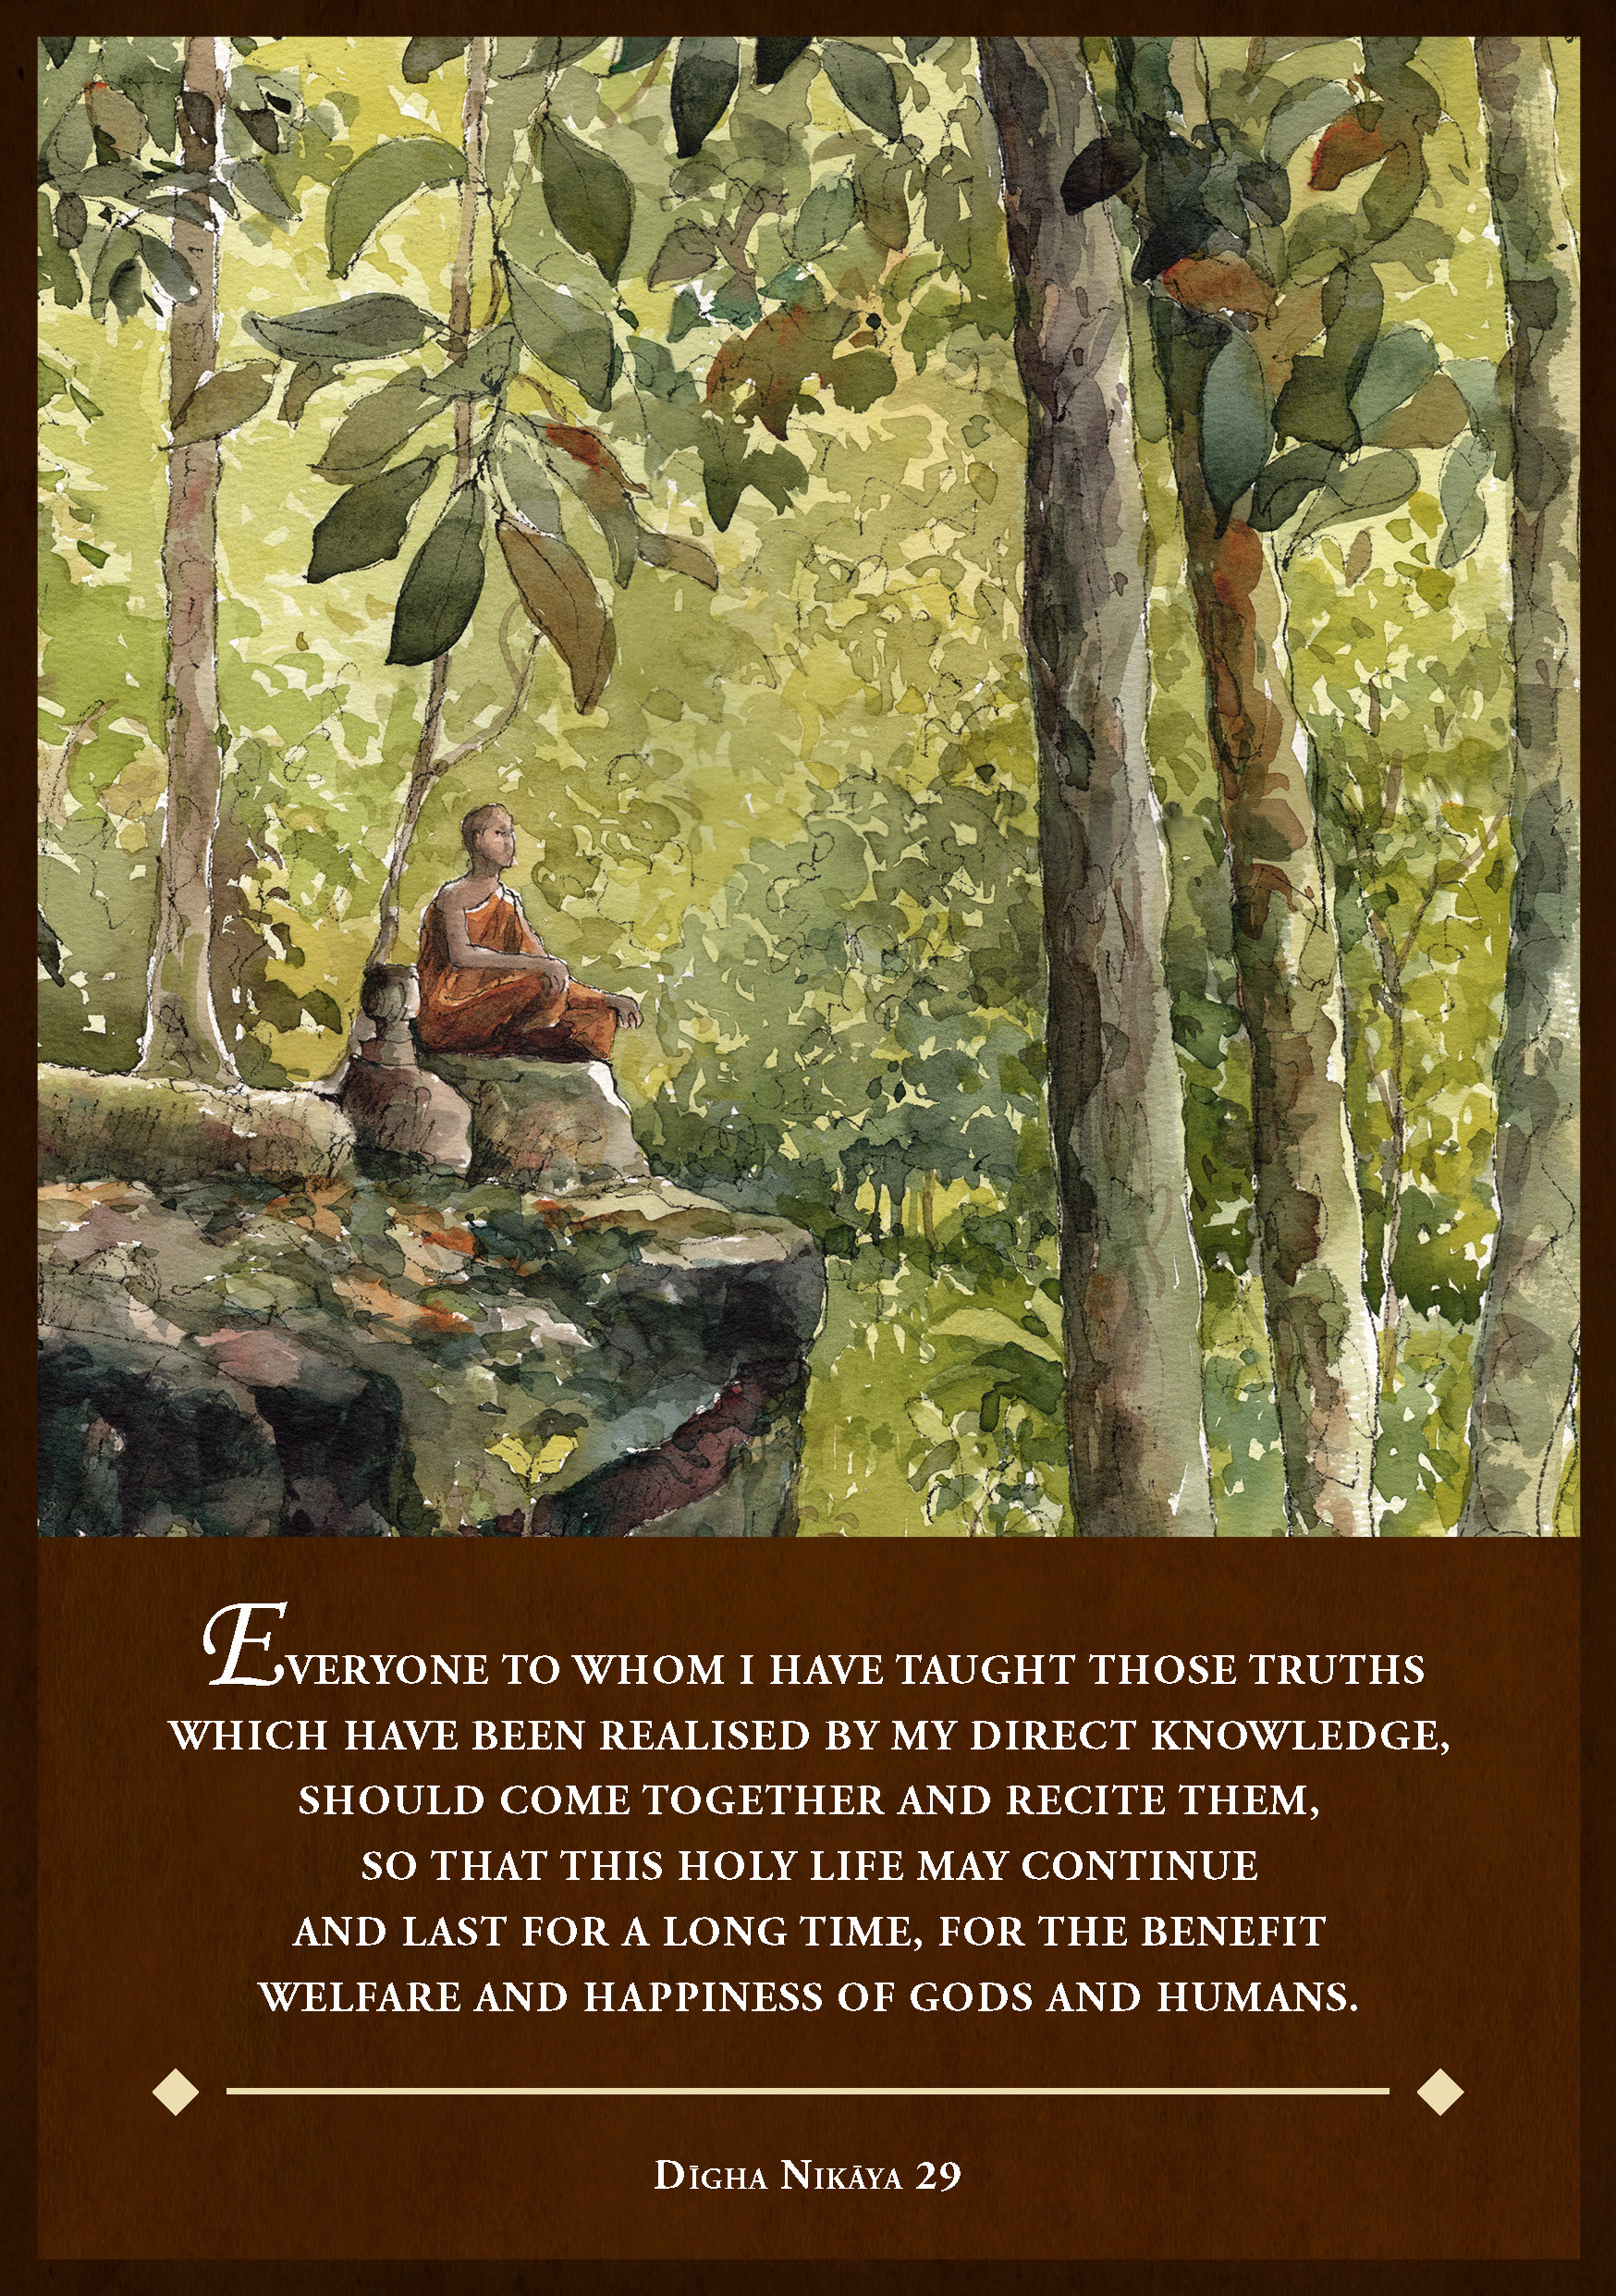
\includegraphics[height=\paperheight]{./assets/images/A5/back_cover_compressed_A5.jpg}}
\fi

\ifninebythirteenversion
  \photoFullBleed{./assets/images/9x13/back_cover_9x13.png}
\fi

\ifbfiveversion
  \photoFullBleed{./assets/images/B5/back_cover_B5.png}
\fi

\end{document}
'
\ifdefined\isdigitalversion
  \newcommand{\digitaloption}{digitalVersion}
\else
  \newcommand{\digitaloption}{}
\fi
\typeout{Set \protect\digitaloption{} to \digitaloption}

% todo ask bergen to make showtims a togglable condition for b5 and 9x13 only

\documentclass[
  final,
  babelLanguage=british,
  showtrims,
  \papersizeoption,
  \digitaloption,
]{anecdote}

% Define graphics path for images
\graphicspath{
  {./assets/images/A5}
  {./assets/images/9x13}
  {./assets/images/B5}
  {./assets/images/graphics}
}

% Loads formatting for selected ddocument class
\ifninebythirteenversion \usepackage{9x13} \fi
\ifafiveversion \usepackage{A5} \fi
\ifbfiveversion \usepackage{B5} \fi

% Set metadata for the document
\title{SBS Pāli-English Recitations}
\subtitle{Monk Training Centre}
\author{SBS Monk Training Centre}
\publisher{Sāsanārakkha Buddhist Sanctuary}
\date{2021-10-30}
\editionInfo{\textit{First Edition}, 2025} % And last edition. Don't call Pāladhammika.
\newcommand{\MyISBN}{} % default empty

\ifbfiveversion
  \renewcommand{\MyISBN}{978-629-97831-1-4}
\fi
\ifninebythirteenversion
  \renewcommand{\MyISBN}{978-629-97831-2-1}
\fi

\ISBN{\MyISBN}

% Set metadata for PDF properties
\hypersetup{
  pdftitle={\thetitle},
  pdfauthor={\theauthor},
  pdfcopyright={Copyright (C) 2025, \thePublisher},
  pdfsubject={},
  pdfkeywords={},
  pdflicenseurl={https://creativecommons.org/licenses/by-nc-nd/4.0/},
  pdfcontacturl={},
  pdflang={en},
}

% Load further packages
\RequirePackage[yyyymmdd,hhmmss]{datetime} % Adds the time to version creation

\makepagenote
\continuousnotenums % Ensure continuous endnote numbering

% Define hyphenation exceptions and corrections
\hyphenation{London re-lin-quishes de-ter-mines}

\ifdigitalversion
  \openany
\fi

% Begin document
\begin{document}

% Front matter
\frontmatter

% Digital version cover
\ifdigitalversion
	\digitalCover{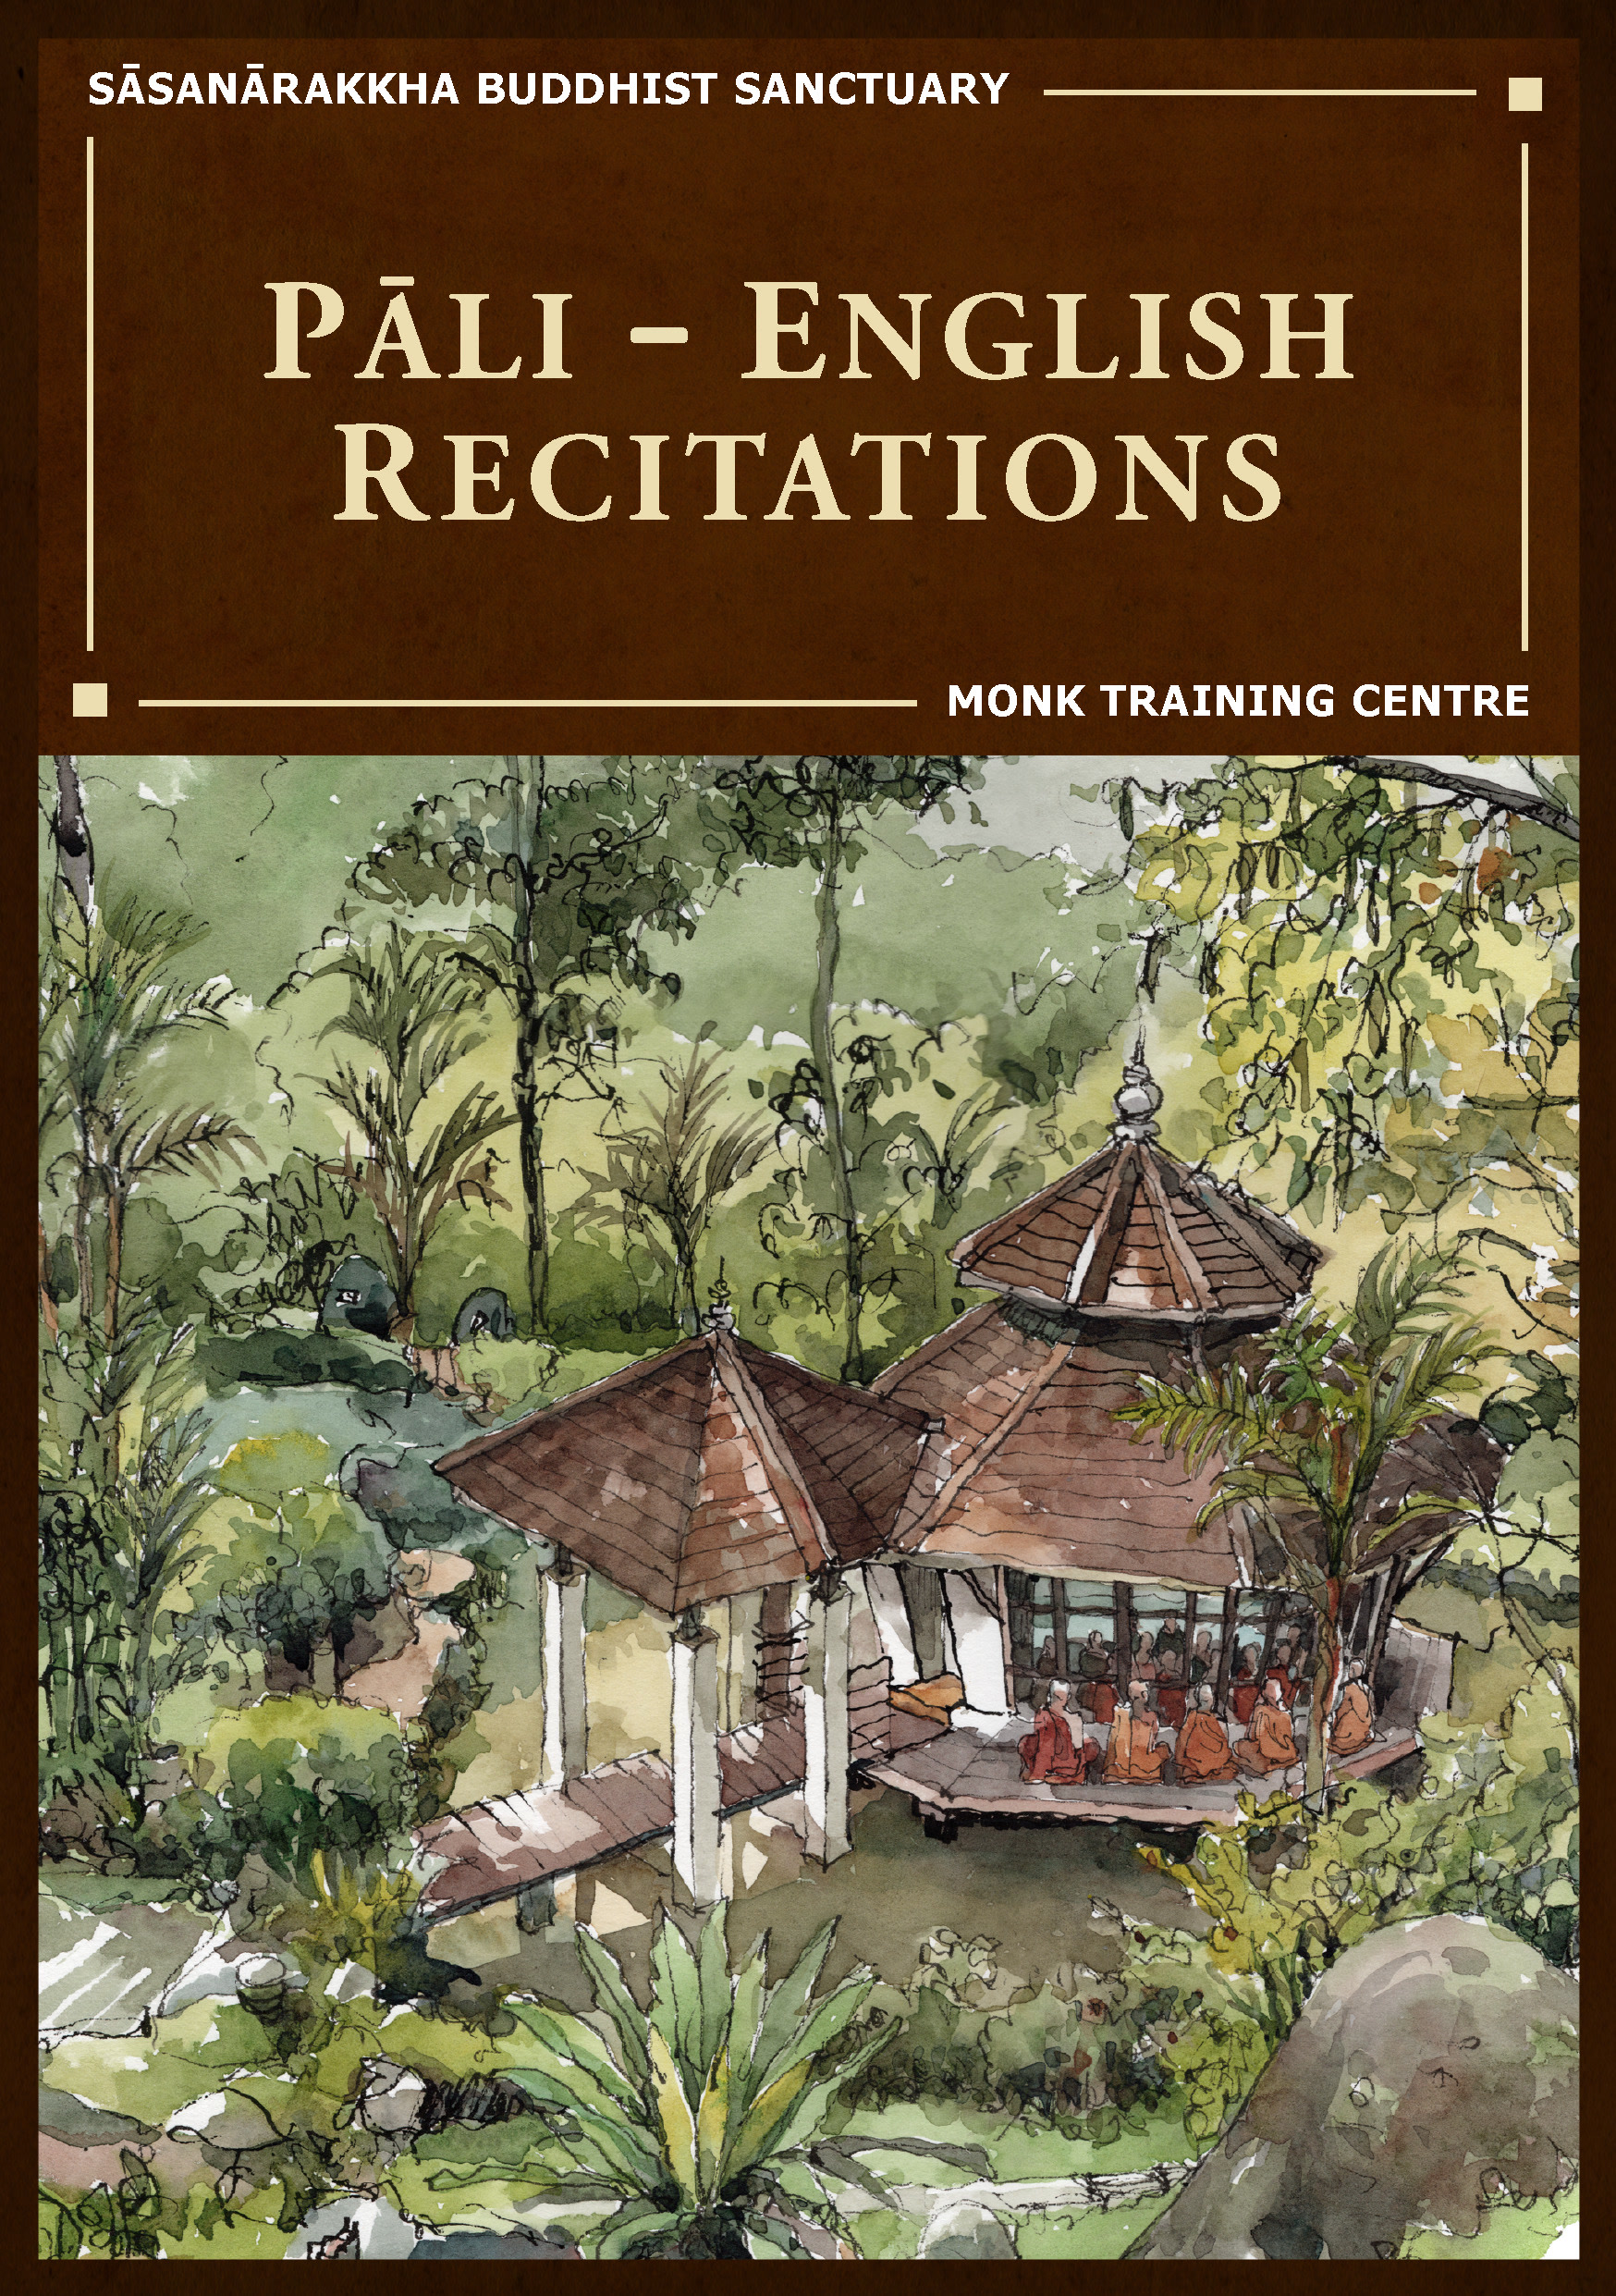
\includegraphics[height=\paperheight]{./assets/images/A5/front_cover_compressed_A5.jpg}}
\fi

\ifninebythirteenversion
  \photoFullBleed{./assets/images/9x13/front_cover_9x13.png}
  \photoFullBleed{robe_divider_left_9x13.png}
  \photoFullBleed{robe_divider_right_9x13.png}
\fi

\ifbfiveversion
  \photoFullBleed{./assets/images/B5/front_cover_B5.png}
  \photoFullBleed{robe_divider_left_B5.png}
  \photoFullBleed{robe_divider_right_B5.png}
\fi

% Title page, copyright, acknowledgments
\pagestyle{empty}

\cleartorecto
\thispagestyle{empty}

\vspace*{3em}

{\centering

  \settowidth{\titleLength}{%
    {\Large\chapterTitleFont\textsc{\MakeUppercase{{Pāli-English Recitations}}}}%
  }

  % 'SBS' on title page
  \ifafive {\Huge\fontsize{64}{16}\sbsFont SBS}\\[1.0\baselineskip] \fi
  \ifninebythirteen {\Huge\fontsize{42.5}{11}\sbsFont SBS}\\[1.0\baselineskip] \fi
  \ifbfive {\Huge\fontsize{80}{16}\sbsFont SBS}\\[1.0\baselineskip] \fi

  % 'Monk Training Centre'
  \ifafive \setlength{\xheight}{\heightof{X}}
    {\Huge\chapterTitleFont\textsc{{\thesubtitle\linebreak}}}\\[0.2\baselineskip] \fi
  \ifninebythirteen {\fontsize{16}{14}\chapterTitleFont\textsc{{\thesubtitle\linebreak}}}\\[0.2\baselineskip] \fi
  \ifbfive \setlength{\xheight}{\heightof{X}}
    {\fontsize{30}{14}\chapterTitleFont\textsc{{\thesubtitle\linebreak}}}\\[0.2\baselineskip] \fi

  % Ornament
  \ifafive \raisebox{0.5\xheight}{\pgfornament[color=sbs-brown,width=7cm,scale=1,ydelta=0pt,symmetry=c]{84}}\\[1.4\baselineskip] \fi
  \ifninebythirteen \raisebox{0.5\xheight}{\pgfornament[color=sbs-brown,width=4.5cm,scale=1,ydelta=0pt,symmetry=c]{84}}\\[1.4\baselineskip] \fi
  \ifbfive \raisebox{0.5\xheight}{\pgfornament[color=sbs-brown,width=8.5cm,scale=1,ydelta=0pt,symmetry=c]{84}}\\[1.4\baselineskip] \fi


  % 'Pali-English Recitations'
  \ifafive {\Large\scshape Pāli-English Recitations}\\[2.5\baselineskip] \fi
  \ifninebythirteen {\fontsize{10}{12}\scshape Pāli-English Recitations}\\[2.5\baselineskip] \fi
  \ifbfive {\fontsize{18.5}{12}\scshape Pāli-English Recitations}\\[2.5\baselineskip] \fi

  % Dhamma quote
  {\quote ``In whatever way a bhikkhu recites the Dhamma in detail as he has heard it and learned it, in just that way, in relation to that Dhamma, he experiences inspiration in the meaning and inspiration in the Dhamma. As he does so, joy arises in him. When he is joyful, rapture arises. For one with a rapturous mind, the body becomes tranquil. One tranquil in body feels pleasure. For one feeling pleasure, the mind becomes concentrated.''\\}
  \ifafive \smallskip AN 5.26\\[1.4\baselineskip]\fi
  \ifninebythirteen \smallskip \fontsize{8}{14}\selectfont AN 5.26\\[1.4\baselineskip]\fi
  %% \ifbfive \smallskip \fontsize{8.5}{14}\selectfont AN 5.26\\[1.4\baselineskip]\fi
  \ifbfive \smallskip AN 5.26\\[1.4\baselineskip]\fi
}



\cleartoverso
\thispagestyle{empty}

{%

  \ifafive \fontsize{10}{16}\selectfont \fi
  \ifninebythirteen \fontsize{7.5}{11}\selectfont \fi
  \ifbfive \fontsize{12}{20}\selectfont \fi
  \centering
  \setlength{\parindent}{0pt}%

  \ifafive \vspace{0.5cm} \fi
  \ifninebythirteen \vspace{0.4cm} \fi
  \ifbfive \vspace{0.5cm} \fi

  \copyright\ \thePublisher, 2025\\
  c/o 160, Lorong 3, Jalan Merdeka, 34000 Taiping, Perak, Malaysia\\
  \ifdigital
    \else
  ISBN \theISBN
  \fi

  \ifafive \vspace{0.5cm} \fi
  \ifninebythirteen \vspace{0.3cm} \fi
  \ifbfive \vspace{0.5cm} \fi

  This book is for free distribution only;\\
  it may not be sold.

  \ifafive \vspace{0.5cm} \fi
  \ifninebythirteen \vspace{0.3cm} \fi
  \ifbfive \vspace{0.5cm} \fi

  Download this book as a PDF, EPUB, MOBI, AZW3\\
  at the following address:\\
  \href{https://sasanarakkha.org/recitations}{https://sasanarakkha.org/recitations}

Accompanying audio recordings can be found at:
\href{https://www.youtube.com/SasanarakkhaBuddhistSanctuary}{https://www.youtube.com/SasanarakkhaBuddhistSanctuary}

  \ifafive \vspace{0.5cm} \fi
  \ifninebythirteen \vspace{0.3cm} \fi
  \ifbfive \vspace{0.5cm} \fi

  Project Manager: Ā. Ariyadhammika\\
  Editor: Ā. Pāladhammika\\
  Typesetting: Aj. Gambhiro, Ā. Pāladhammika\\
  Translators: Ā. Aggacitta, Ā. Bodhi, Aj. Kevalī, Ā. Sujāto, M. Walshe\\
  Endnotes: Ā. Ariyadhammika\\
  Watercolor Paintings: Lim Jee Yuan

  \ifafive \vspace{0.5cm} \fi
  \ifninebythirteen \vspace{0.3cm} \fi
  \ifbfive \vspace{0.5cm} \fi

  This work is licensed under a Creative Commons\\
  Attribution-NonCommercial-NoDerivatives 4.0 International~License.

  % Produced with the \LaTeX\ typesetting system,\\
  % set in Libertinus Serif.

  \ifafive  \vspace{0.5cm} \fi
  \ifninebythirteen \vspace{0.3cm} \fi
  \ifbfive \vspace{0.5cm} \fi

  \ifdigital
    This version was created on:\\
    \today \space at \currenttime\\
  \fi

  \ifafive \vspace{0.5cm} \fi
  \ifninebythirteen \vspace{0.15cm} \fi
  \ifbfive \vspace{0.5cm} \fi

  \theEditionInfo

}

\ifdigital

\else

\clearpage

\fi



\cleartorecto
\thispagestyle{empty}

{

  \setlength{\parskip}{10pt}

  \ifafive {\centering\fontsize{16}{25}\selectfont \textsc{We Wish To Gratefully Acknowledge} \par} \fi
  \ifninebythirteen {\centering\fontsize{10}{18}\selectfont \textsc{We Wish To Gratefully Acknowledge} \par} \fi
  \ifbfive {\centering\fontsize{18.5}{25}\selectfont \textsc{We Wish To Gratefully Acknowledge} \par} \fi


  The Saṅghas of Wat Pah Nanachat (WPN), Amaravati, and Abhayagiri for allowing the use of material from their respective chanting books, the late Ven. Dr. Saddhātissa and Mr. Maurice Walshe for their English translations, as well as Ven. Bhikkhu Bodhi for granting permission to use and slightly adapt his translations. Various Saṅgha members of SBS Monk Training Centre, who contributed in the compilation of an interesting selection of chants, as well as for providing countless suggestions to help improve the English translations.

  \linkdest{endnote1-body}
  Additional information on translations, as well as deviations\makeatletter\hyperlink{endnote1-appendix}\Hy@raisedlink{{\pagenote{%
        \hypertarget{endnote1-appendix}{\hyperlink{endnote1-body}{Due to the balanced and inspiring selection of chants, as well as for the sake of compatibility, WPN’s \textit{Buddhist Chanting} (2014) has served as the basis for this book. Over time, suggestions for the inclusion of additional chants, as well as occasional improvements of existing translations were incorporated. Such changes were meticulously marked down in the endnotes of the digital versions of this chanting book, so that someone familiar with the present book can straight away find the relevant differences, which can be useful when visiting a branch monastery of the Ajahn Chah lineage, in order to know in which places to revert to the original version.}}}}}\makeatother\thickspace
  from WPN's \textit{Buddhist Chanting} (2014), have been annotated by Ven. Ariyadhammika in the endnotes.


  \ifninebythirteen \smallskip \else \medskip \fi

  {\centering

    To Āyasmā Aggacitta, the founding father of\\
    Sāsanārakkha Buddhist Sanctuary.

    % \ifninebythirteen \smallskip \else \medskip \fi

    \begin{center}
      \ifafive 
\includegraphics[height=54mm]{sbs_logo_tuck_loon_brown.jpg} \fi
      \ifninebythirteen \clearpage \vspace*{\fill}
 
\includegraphics[height=80mm]{sbs_logo_tuck_loon_brown.jpg} \vspace*{\fill} \fi
      \ifbfive \vspace{1cm} 
\includegraphics[height=70mm]{sbs_logo_tuck_loon_brown.jpg}\fi
    \end{center}
  }
}



% Table of contents, schedule, purpose and benefits, abbreviations
\cleartorecto
\pagestyle{toponerow-frontmatter}
\chapterstyle{adrasteia-toc}

\pdfbookmark[section]{\contentsname}{toc}
\tableofcontents*


\chapter{Recitation Schedule}
\label{schedule}

{\centering

  {\pdfbookmark[2]{Set 1}{set1}\libertinusFont\selectfont\textbf{\textsc{\ifafive\fontsize{18}{12}\fi\ifninebythirteen\fontsize{13}{8.5}\fi\ifbfive\fontsize{22}{18}\fi\selectfont\textls*{Set 1}}}}\\
  \textsc{\ifafive\fontsize{14.4}{28}\fi\ifninebythirteen\fontsize{8.7}{17}\fi\ifbfive\fontsize{16}{33.5}\fi\selectfont
    \hyperref[buddhas-first-exclamation]{The Buddha's First Exclamation} \ifdigital\else\pageref{buddhas-first-exclamation}\fi\\
    \hyperref[wheel-of-dhamma-abridged]{Turning the Wheel of Dhamma} \ifdigital\else\pageref{wheel-of-dhamma-abridged}\fi\\
    \hyperref[true-false-refuges]{Going to True and False Refuges} \ifdigital\else\pageref{true-false-refuges}\fi\\
    \hyperref[four-great-references]{The Four Great References} \ifdigital\else\pageref{four-great-references}\fi\\
    \hyperref[patimokkha-exhortation]{The Pāṭimokkha Exhortation} \ifdigital\else\pageref{patimokkha-exhortation}\fi\\
    \hyperref[buddhas-final-instruction]{The Buddha's Final Instruction} \ifdigital\else\pageref{buddhas-final-instruction}\fi\\
    \hyperref[uddissanadhitthana]{Sharing and Aspirations (Pāli)} \ifdigital\else\pageref{uddissanadhitthana}\fi\\
    \hyperref[closing-homage]{Closing Homage (Pāli-English)} \ifdigital\else\pageref{closing-homage}\fi\\
  }

  \ifafive\vspace{1.0cm}\fi
  \ifninebythirteen\vspace{0.8cm}\fi
  \ifbfive\vspace{1.0cm}\fi

  {\pdfbookmark[2]{Set 2}{set2}\libertinusFont\selectfont\textbf{\textsc{\ifafive\fontsize{18}{12}\fi\ifninebythirteen\fontsize{13}{8.5}\fi\ifbfive\fontsize{22}{18}\fi\selectfont\textls*{Set 2}}}}\\
  \textsc{\ifafive\fontsize{14.4}{28}\fi\ifninebythirteen\fontsize{8.7}{17}\fi\ifbfive\fontsize{16}{33.5}\fi\selectfont
    \hyperref[characteristic-of-not-self]{The Discourse on the Characteristic of Not-Self} \ifdigital\else\pageref{characteristic-of-not-self}\fi\\
    \hyperref[exposition-on-burning]{The Discourse on the Exposition on Burning} \ifdigital\else\pageref{exposition-on-burning}\fi\\
    \hyperref[gradual-training]{The Gradual Training} \ifdigital\else\pageref{gradual-training}\fi\\
    \hyperref[sharing-aspirations]{Sharing and Aspirations (English)} \ifdigital\else\pageref{sharing-aspirations}\fi\\
    \hyperref[closing-homage]{Closing Homage (English)} \ifdigital\else\pageref{closing-homage}\fi\\
  }

  \clearpage

  {\pdfbookmark[2]{Set 3}{set3}\libertinusFont\selectfont\textbf{\textsc{\ifafive\fontsize{18}{12}\fi\ifninebythirteen\fontsize{13}{8.5}\fi\ifbfive\fontsize{22}{18}\fi\selectfont\textls*{Set 3}}}}\\

\textsc{\ifafive\fontsize{14.4}{28}\fi\ifninebythirteen\fontsize{8.7}{17}\fi\ifbfive\fontsize{16}{33.5}\fi\selectfont
    \hyperref[noble-eightfold-path]{The Noble Eightfold Path} \ifdigital\else\pageref{noble-eightfold-path}\fi\\
    \hyperref[repulsiveness-of-food]{The Repulsiveness of Food} \ifdigital\else\pageref{repulsiveness-of-food}\fi\\
    \hyperref[requisites-for-awakening]{Requisites for Awakening} \ifdigital\else\pageref{requisites-for-awakening}\fi\\
    \hyperref[principles-of-non-decline]{Principles of Non-Decline} \ifdigital\else\pageref{principles-of-non-decline}\fi\\
    \hyperref[protection]{On Protection} \ifdigital\else\pageref{protection}\fi\\
    \hyperref[sharing-all-merits]{Sharing of All Merits} \ifdigital\else\pageref{sharing-all-merits}\fi\\
    \hyperref[closing-homage]{Closing Homage (Pāli-English)} \ifdigital\else\pageref{closing-homage}\fi\\
  }

  \ifafive\vspace{1.0cm}\fi
  \ifninebythirteen\vspace{0.8cm}\fi
  \ifbfive\vspace{1.0cm}\fi

  {\pdfbookmark[2]{Set 4}{set4}\libertinusFont\selectfont\textbf{\textsc{\ifafive\fontsize{18}{12}\fi\ifninebythirteen\fontsize{13}{8.5}\fi\ifbfive\fontsize{22}{18}\fi\selectfont\textls*{Set 4}}}}\\

\textsc{\ifafive\fontsize{14.4}{28}\fi\ifninebythirteen\fontsize{8.7}{17}\fi\ifbfive\fontsize{16}{33.5}\fi\selectfont
    \hyperref[dedication-of-offerings]{Homage to the Triple Gem} \ifdigital\else\pageref{dedication-of-offerings}\fi\\
    \hyperref[universal-well-being]{Universal Well-Being} \ifdigital\else\pageref{universal-well-being}\fi\\
    \hyperref[seven-factors-of-awakening]{The Seven Factors of Awakening} \ifdigital\else\pageref{seven-factors-of-awakening}\fi\\
    \hyperref[words-on-loving-kindness]{The Buddha's Words on Loving-Kindness} \ifdigital\else\pageref{words-on-loving-kindness}\fi\\
    \hyperref[sharing-merits-departed]{Sharing of Merits with \ifninebythirteen\\[-0.6em]\fi the Departed (Pāli-English)} \ifdigital\else\pageref{sharing-merits-departed}\fi\\
    \hyperref[sharing-merits-devas]{Sharing of Merits with the Devas (Pāli-English)} \ifdigital\else\pageref{sharing-merits-devas}\fi\\
    \hyperref[closing-homage]{Closing Homage (Pāli-English)} \ifdigital\else\pageref{closing-homage}\fi\\
  }

  \clearpage

  {\pdfbookmark[2]{Set 5}{set5}\libertinusFont\selectfont\textbf{\textsc{\ifafive\fontsize{18}{12}\fi\ifninebythirteen\fontsize{13}{8.5}\fi\ifbfive\fontsize{22}{18}\fi\selectfont\textls*{Set 5}}}}\\
  \textsc{\ifafive\fontsize{14.4}{28}\fi\ifninebythirteen\fontsize{8.7}{17}\fi\ifbfive\fontsize{16}{33.5}\fi\selectfont
    \hyperref[mindfulness-of-breathing]{Mindfulness of Breathing} \ifdigital\else\pageref{mindfulness-of-breathing}\fi\\
    \hyperref[discourse-on-blessings]{The Discourse on Blessings} \ifdigital\else\pageref{discourse-on-blessings}\fi\\
    \hyperref[three-characteristics]{The Three Characteristics} \ifdigital\else\pageref{three-characteristics}\fi\\
    \hyperref[four-requisites]{The Four Requisites} \ifdigital\else\pageref{four-requisites}\fi\\
    \hyperref[five-reflections]{Five Subjects for Frequent Reflection} \ifdigital\else\pageref{five-reflections}\fi\\
    \hyperref[32-parts]{The Thirty-Two Body Parts} \ifdigital\else\pageref{32-parts}\fi\\
    \hyperref[principles-of-cordiality]{Principles of Cordiality} \ifdigital\else\pageref{principles-of-cordiality}\fi\\
    \hyperref[highest-honour-aspirations]{The Highest Honour and Aspirations} \ifdigital\else\pageref{highest-honour-aspirations}\fi\\
    \hyperref[closing-homage]{Closing Homage (Pāli-English)} \ifdigital\else\pageref{closing-homage}\fi\\
  }

  \ifafive\vspace{1.0cm}\fi
  \ifninebythirteen\vspace{0.8cm}\fi
  \ifbfive\vspace{1.0cm}\fi

  {\pdfbookmark[2]{Set 6}{set6}\libertinusFont\selectfont\textbf{\textsc{\ifafive\fontsize{18}{12}\fi\ifninebythirteen\fontsize{13}{8.5}\fi\ifbfive\fontsize{22}{18}\fi\selectfont\textls*{Set 6}}}}\\
  \textsc{\ifafive\fontsize{14.4}{28}\fi\ifninebythirteen\fontsize{8.7}{17}\fi\ifbfive\fontsize{16}{33.5}\fi\selectfont
    \hyperref[anatta-lakkhana]{Anatta-lakkhaṇa Sutta} \ifdigital\else\pageref{anatta-lakkhana}\fi\\
    \hyperref[striving-according-to-dhamma]{Striving According to the Dhamma} \ifdigital\else\pageref{striving-according-to-dhamma}\fi\\
    \hyperref[divine-abidings]{The Divine Abidings} \ifdigital\else\pageref{divine-abidings}\fi\\
    \hyperref[ten-reflections]{Ten Subjects for Frequent Reflection\\ \ifafive\vspace{-0.4cm}\fi \ifbfive\vspace{-0.4cm}\fi \ifninebythirteen\vspace{-0.2cm}\fi by One Gone Forth} \ifdigital\else\pageref{ten-reflections}\fi\\
    \hyperref[sharing-aspirations]{Sharing and Aspirations (English)} \ifdigital\else\pageref{sharing-aspirations}\fi\\
    \hyperref[closing-homage]{Closing Homage (Pāli-English)} \ifdigital\else\pageref{closing-homage}\fi\\
  }

  \clearpage

  {\pdfbookmark[2]{Set 7}{set7}\libertinusFont\selectfont\textbf{\textsc{\ifafive\fontsize{18}{12}\fi\ifninebythirteen\fontsize{13}{8.5}\fi\ifbfive\fontsize{22}{18}\fi\selectfont\textls*{Set 7}}}}\\
  \textsc{\ifafive\fontsize{14.4}{28}\fi\ifninebythirteen\fontsize{8.7}{17}\fi\ifbfive\fontsize{16}{33.5}\fi\selectfont
    \hyperref[dependent-origination]{Dependent Origination} \ifdigital\else\pageref{dependent-origination}\fi\\
    \hyperref[dhamma-in-brief]{The Dhamma in Brief} \ifdigital\else\pageref{dhamma-in-brief}\fi\\
    \hyperref[uddissanadhitthana]{Sharing and Aspirations (Pāli)} \ifdigital\else\pageref{uddissanadhitthana}\fi\\
    \hyperref[closing-homage]{Closing Homage (Pāli-English)} \ifdigital\else\pageref{closing-homage}\fi\\
  }

  \ifafive\vspace{1.0cm}\fi
  \ifninebythirteen\vspace{0.8cm}\fi
  \ifbfive\vspace{1.0cm}\fi

  {\pdfbookmark[2]{Set 8}{set8}\libertinusFont\selectfont\textbf{\textsc{\ifafive\fontsize{18}{12}\fi\ifninebythirteen\fontsize{13}{8.5}\fi\ifbfive\fontsize{22}{18}\fi\selectfont\textls*{Set 8}}}}\\
  \textsc{\ifafive\fontsize{14.4}{28}\fi\ifninebythirteen\fontsize{8.7}{17}\fi\ifbfive\fontsize{16}{33.5}\fi\selectfont
    \hyperref[aditta-pariyaya]{Āditta-Pariyāya Sutta} \ifdigital\else\pageref{aditta-pariyaya}\fi\\
    \hyperref[burdens]{The Burdens} \ifdigital\else\pageref{burdens}\fi\\
    \hyperref[respect-for-the-dhamma]{Respect for the Dhamma} \ifdigital\else\pageref{respect-for-the-dhamma}\fi\\
    \hyperref[single-excellent-night]{A Single Excellent Night} \ifdigital\else\pageref{single-excellent-night}\fi\\
    \hyperref[ratthapala]{From the Elder Raṭṭhapāla}  \ifdigital\else\pageref{ratthapala}\fi\\
    \hyperref[parapariya]{From the Elder Pārāpariya} \ifdigital\else\pageref{parapariya}\fi\\
    \hyperref[misc-verses]{Miscellaneous Verses} \ifdigital\else\pageref{misc-verses}\fi\\
    \hyperref[highest-honour-aspirations]{The Highest Honour and Aspirations} \ifdigital\else\pageref{highest-honour-aspirations}\fi\\
    \hyperref[closing-homage]{Closing Homage (Pāli-English)} \ifdigital\else\pageref{closing-homage}\fi\\
  }

  \clearpage

  {\pdfbookmark[2]{Set 9}{set9}\libertinusFont\selectfont\textbf{\textsc{\ifafive\fontsize{18}{12}\fi\ifninebythirteen\fontsize{13}{8.5}\fi\ifbfive\fontsize{22}{18}\fi\selectfont\textls*{Set 9}}}}\\
  \textsc{\ifafive\fontsize{14.4}{28}\fi\ifninebythirteen\fontsize{8.7}{17}\fi\ifbfive\fontsize{16}{33.5}\fi\selectfont
    \hyperref[invitation-to-the-devas]{Protective Recitations (Pāli)} \ifdigital\else\pageref{invitation-to-the-devas}\fi\\
    \hyperref[sharing-merits-departed]{Sharing of Merits with the Departed (Pāli)} \ifdigital\else\pageref{sharing-merits-departed}\fi\\
    \hyperref[sharing-merits-devas]{Sharing of Merits with the Devas (Pāli)} \ifdigital\else\pageref{sharing-merits-devas}\fi\\
    \hyperref[closing-homage]{Closing Homage (Pāli)} \ifdigital\else\pageref{closing-homage}\fi\\
  }

  \ifafive\vspace{1.0cm}\fi
  \ifninebythirteen\vspace{0.8cm}\fi
  \ifbfive\vspace{1.0cm}\fi

  {\pdfbookmark[2]{Set 10}{set10}\libertinusFont\selectfont\textbf{\textsc{\ifafive\fontsize{18}{12}\fi\ifninebythirteen\fontsize{13}{8.5}\fi\ifbfive\fontsize{22}{18}\fi\selectfont\textls*{Set 10}}}}\\
\textsc{\ifafive\fontsize{14.4}{28}\fi\ifninebythirteen\fontsize{8.7}{17}\fi\ifbfive\fontsize{16}{33.5}\fi\selectfont
    \hyperref[passage-on-preliminary-paying-of-homage-funeral]{Funeral Recitations (Pāli)} \ifdigital\else\pageref{passage-on-preliminary-paying-of-homage-funeral}\fi\\
    \hyperref[recollection-of-impermanence]{Recollection of Impermanence} \ifdigital\else\pageref{recollection-of-impermanence}\fi\\
    \hyperref[just-as-rivers]{Thanksgiving Recitations} \ifdigital\else\pageref{just-as-rivers}\fi\\
    \hyperref[sharing-all-merits]{Sharing of All Merits} \ifdigital\else\pageref{sharing-all-merits}\fi\\
    \hyperref[closing-homage]{Closing Homage (Pāli-English)} \ifdigital\else\pageref{closing-homage}\fi\\
  }}


\input{./tex/purpose-and-benefits.tex}

\chapter{Abbreviations}
\label{abbreviations}

\ifafive
\begin{tabular}{@{}ll@{}}
  \anglebracketleft\ \hspace{-0.5mm}... \hspace{-0.85mm}\anglebracketright\ & \hspace{1.30mm}Only recited by the leader \\
  \hspace{0.1cm} \abbrbreathmark\ & \hspace{1.45mm}Breathing pause \\
\end{tabular}
\fi

\ifninebythirteen
\begin{tabular}{@{}ll@{}}
  \anglebracketleft\ \hspace{-0.5mm}... \hspace{-0.70mm}\anglebracketright\ & \hspace{1.10mm}Only recited by the leader \\
  \hspace{0.1cm} \abbrbreathmark\ & \hspace{1.20mm}Breathing pause \\
\end{tabular}
\fi

\ifbfive
\begin{tabular}{@{}ll@{}}
  \anglebracketleft\ \hspace{-0.5mm}... \hspace{-0.85mm}\anglebracketright\ & \hspace{2.70mm}Only recited by the leader \\
  \hspace{0.2cm} \abbrbreathmark\ & \hspace{2.90mm}Breathing pause \\
\end{tabular}
\fi

\ifninebythirteen

\vspace{-0.6em}
\begin{tabular}{@{}llll@{}}
  DN    & Dīgha Nikāya                                        \\
  MN    & Majjhima Nikāya                                     \\
  SN    & Saṁyutta Nikāya                                     \\
  AN    & Aṅguttara Nikāya                                    \\
  Kp    & Khuddakapāṭha                                       \\
  Dhp   & Dhammapada                                          \\
  Ud    & Udāna                                               \\
  Snp   & Sutta Nipāta                                        \\
  Thag  & Theragāthā                                          \\
  Ja    & Jātaka                                              \\
  Pv    & Petavatthu                                          \\
  Vibh  & Abhidhamma Vibhaṅga                                 \\
  Dhs   & Dhammasaṅganī                                       \\
  A     & Aṭṭhakathā (Commentary)                             \\
  MJG   & Mahā-jaya-maṅgala-gāthā (Sri Lanka)                 \\
  Trad  & Traditional post-canonical verses                   \\
  WPN   & Wat Pah Nanachat                                    \\
\end{tabular}

\else

\begin{tabular}{@{}llll@{}}
  DN    & Dīgha Nikāya                                        \\
  MN    & Majjhima Nikāya                                     \\
  SN    & Saṁyutta Nikāya                                     \\
  AN    & Aṅguttara Nikāya                                    \\
  Kp    & Khuddakapāṭha                                       \\
  Dhp   & Dhammapada                                          \\
  Ud    & Udāna                                               \\
  Snp   & Sutta Nipāta                                        \\
  Thag  & Theragāthā                                          \\
  Ja    & Jātaka                                              \\
  Pv    & Petavatthu                                          \\
  Vibh  & Abhidhamma Vibhaṅga                                 \\
  Dhs   & Dhammasaṅganī                                       \\
\end{tabular}

\begin{tabular}{@{}llll@{}}
  A     & Aṭṭhakathā (Commentary)                             \\
  MJG   & Mahā-jaya-maṅgala-gāthā (Sri Lanka)                 \\
  Trad  & Traditional post-canonical verses                   \\
  WPN   & Wat Pah Nanachat
\end{tabular}

\medskip

\fi



\chapterstyle{adrasteia-frontmatter}

% Main matter
\mainmatter
\pagestyle{toponerow}

\cleartorecto

% Chapters
{\raggedright
	\input{./tex/recitations/homage.tex}
	\input{./tex/recitations/verses.tex}
	\input{./tex/recitations/teachings.tex}
	\input{./tex/recitations/reflections.tex}
	
\ifdigitalversion
  \chapterOpeningPage{cardinal_discourses_compressed_A5.jpg}
\else
  \chapterOpeningPage{cardinal_discourses_A5.jpg}
\fi

\ifninebythirteenversion
  \chapterOpeningPage{cardinal_discourses_9x13.png}
\fi

\ifbfiveversion
  \chapterOpeningPage{cardinal_discourses_B5.png}
\fi

\chapter{Cardinal Discourses}

\ifbfiveversion
  \photoFullBleed{assets/images/B5/brown_divider_B5.pdf}
\fi

\ifninebythirteenversion
  \photoFullBleed{assets/images/9x13/brown_divider_9x13.pdf}\fi

\input{./tex/recitations/cardinal-discourses/dhammacakkappavattana.tex}

\clearpage

\input{./tex/recitations/cardinal-discourses/dhammacakkappavattana-eng.tex}

\clearpage

\input{./tex/recitations/cardinal-discourses/anattalakkhana.tex}

\clearpage

\input{./tex/recitations/cardinal-discourses/anattalakkhana-eng.tex}

\clearpage

\input{./tex/recitations/cardinal-discourses/adittapariyaya.tex}

\clearpage

\input{./tex/recitations/cardinal-discourses/adittapariyaya-eng.tex}

\clearpage


	\input{./tex/recitations/thanksgiving-recitations.tex}
	\input{./tex/recitations/protective-recitations.tex}
	\input{./tex/recitations/funeral-recitations.tex}
	\input{./tex/recitations/sharing-of-merits.tex}
}

% Appendix
\appendix

\ifdigitalversion
  \chapterOpeningPage{appendix_compressed_A5.jpg}
\else
  \chapterOpeningPage{appendix_A5.jpg}
\fi

\ifninebythirteenversion
  \chapterOpeningPage{appendix_9x13.jpg}
\fi

\ifbfiveversion
  \chapterOpeningPage{appendix_B5.jpg}
\fi

\ifafiveversion\addtocontents{toc}{\protect\clearpage}\fi
\chapter{Appendix}

\ifbfiveversion
  \includepdf[pages=-]{assets/graphics/brown-texture_B5.pdf}
\fi

\ifninebythirteenversion
  \includepdf[pages=-]{assets/graphics/brown-texture_9x13.pdf}
\fi

\clearpage


\input{./tex/refuge-trainings.tex}
\input{./tex/phonetics-pronunciation.tex}
\input{./tex/guidelines.tex}

% Back matter
\backmatter
\printpagenotes % Print endnotes
\input{./tex/copyright-details.tex}

\ifbfiveversion
  \includepdf[pages=-,pagecommand={\thispagestyle{empty}}]{assets/images/graphics/donor-list.pdf}
  \photoFullBleed{robe_divider_left_B5.png}
  \photoFullBleed{robe_divider_right_B5.png}
\fi

\ifninebythirteenversion
  \photoFullBleed{robe_divider_left_9x13.png}
  \photoFullBleed{robe_divider_right_9x13.png}
\fi

\emptyUntilEven % Add blank page if necessary

\ifdigitalversion
  \clearpage
  \digitalCover{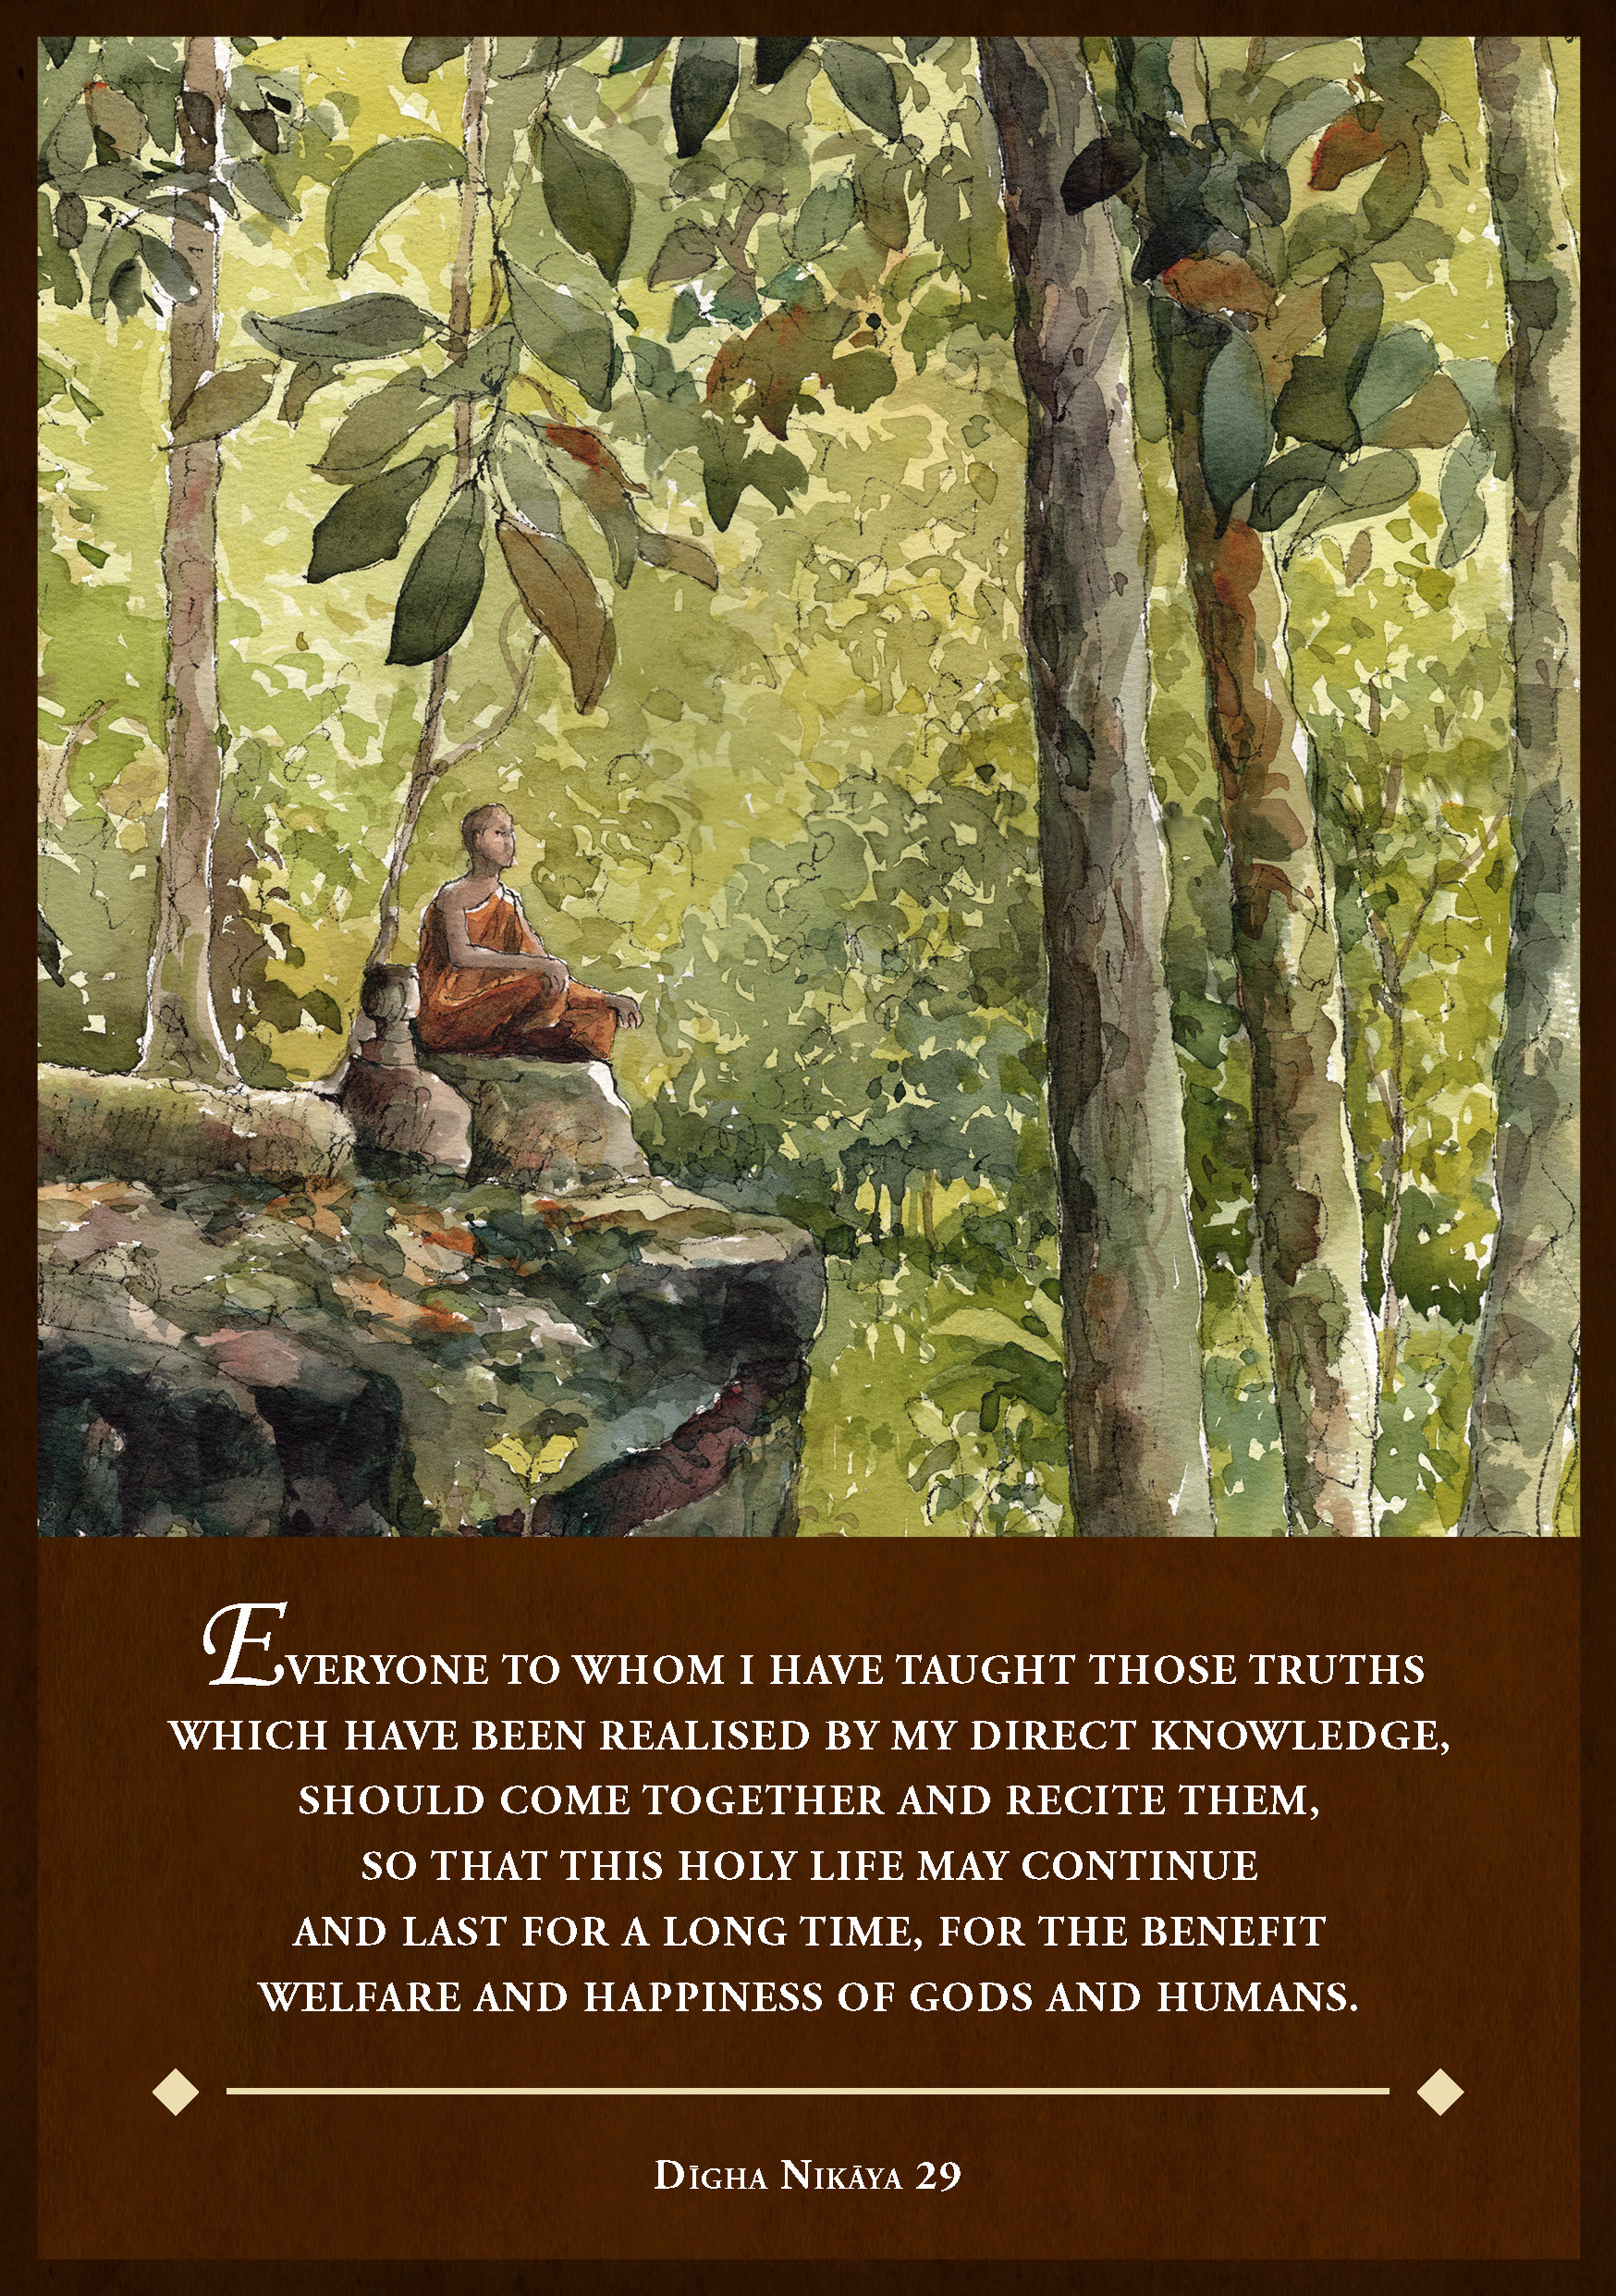
\includegraphics[height=\paperheight]{./assets/images/A5/back_cover_compressed_A5.jpg}}
\fi

\ifninebythirteenversion
  \photoFullBleed{./assets/images/9x13/back_cover_9x13.png}
\fi

\ifbfiveversion
  \photoFullBleed{./assets/images/B5/back_cover_B5.png}
\fi

\end{document}
'
\ifdefined\isdigitalversion
  \newcommand{\digitaloption}{digitalVersion}
\else
  \newcommand{\digitaloption}{}
\fi
\typeout{Set \protect\digitaloption{} to \digitaloption}

% todo ask bergen to make showtims a togglable condition for b5 and 9x13 only

\documentclass[
  final,
  babelLanguage=british,
  showtrims,
  \papersizeoption,
  \digitaloption,
]{anecdote}

% Define graphics path for images
\graphicspath{
  {./assets/images/A5}
  {./assets/images/9x13}
  {./assets/images/B5}
  {./assets/images/graphics}
}

% Loads formatting for selected ddocument class
\ifninebythirteenversion \usepackage{9x13} \fi
\ifafiveversion \usepackage{A5} \fi
\ifbfiveversion \usepackage{B5} \fi

% Set metadata for the document
\title{SBS Pāli-English Recitations}
\subtitle{Monk Training Centre}
\author{SBS Monk Training Centre}
\publisher{Sāsanārakkha Buddhist Sanctuary}
\date{2021-10-30}
\editionInfo{\textit{First Edition}, 2025} % And last edition. Don't call Pāladhammika.
\newcommand{\MyISBN}{} % default empty

\ifbfiveversion
  \renewcommand{\MyISBN}{978-629-97831-1-4}
\fi
\ifninebythirteenversion
  \renewcommand{\MyISBN}{978-629-97831-2-1}
\fi

\ISBN{\MyISBN}

% Set metadata for PDF properties
\hypersetup{
  pdftitle={\thetitle},
  pdfauthor={\theauthor},
  pdfcopyright={Copyright (C) 2025, \thePublisher},
  pdfsubject={},
  pdfkeywords={},
  pdflicenseurl={https://creativecommons.org/licenses/by-nc-nd/4.0/},
  pdfcontacturl={},
  pdflang={en},
}

% Load further packages
\RequirePackage[yyyymmdd,hhmmss]{datetime} % Adds the time to version creation

\makepagenote
\continuousnotenums % Ensure continuous endnote numbering

% Define hyphenation exceptions and corrections
\hyphenation{London re-lin-quishes de-ter-mines}

\ifdigitalversion
  \openany
\fi

% Begin document
\begin{document}

% Front matter
\frontmatter

% Digital version cover
\ifdigitalversion
	\digitalCover{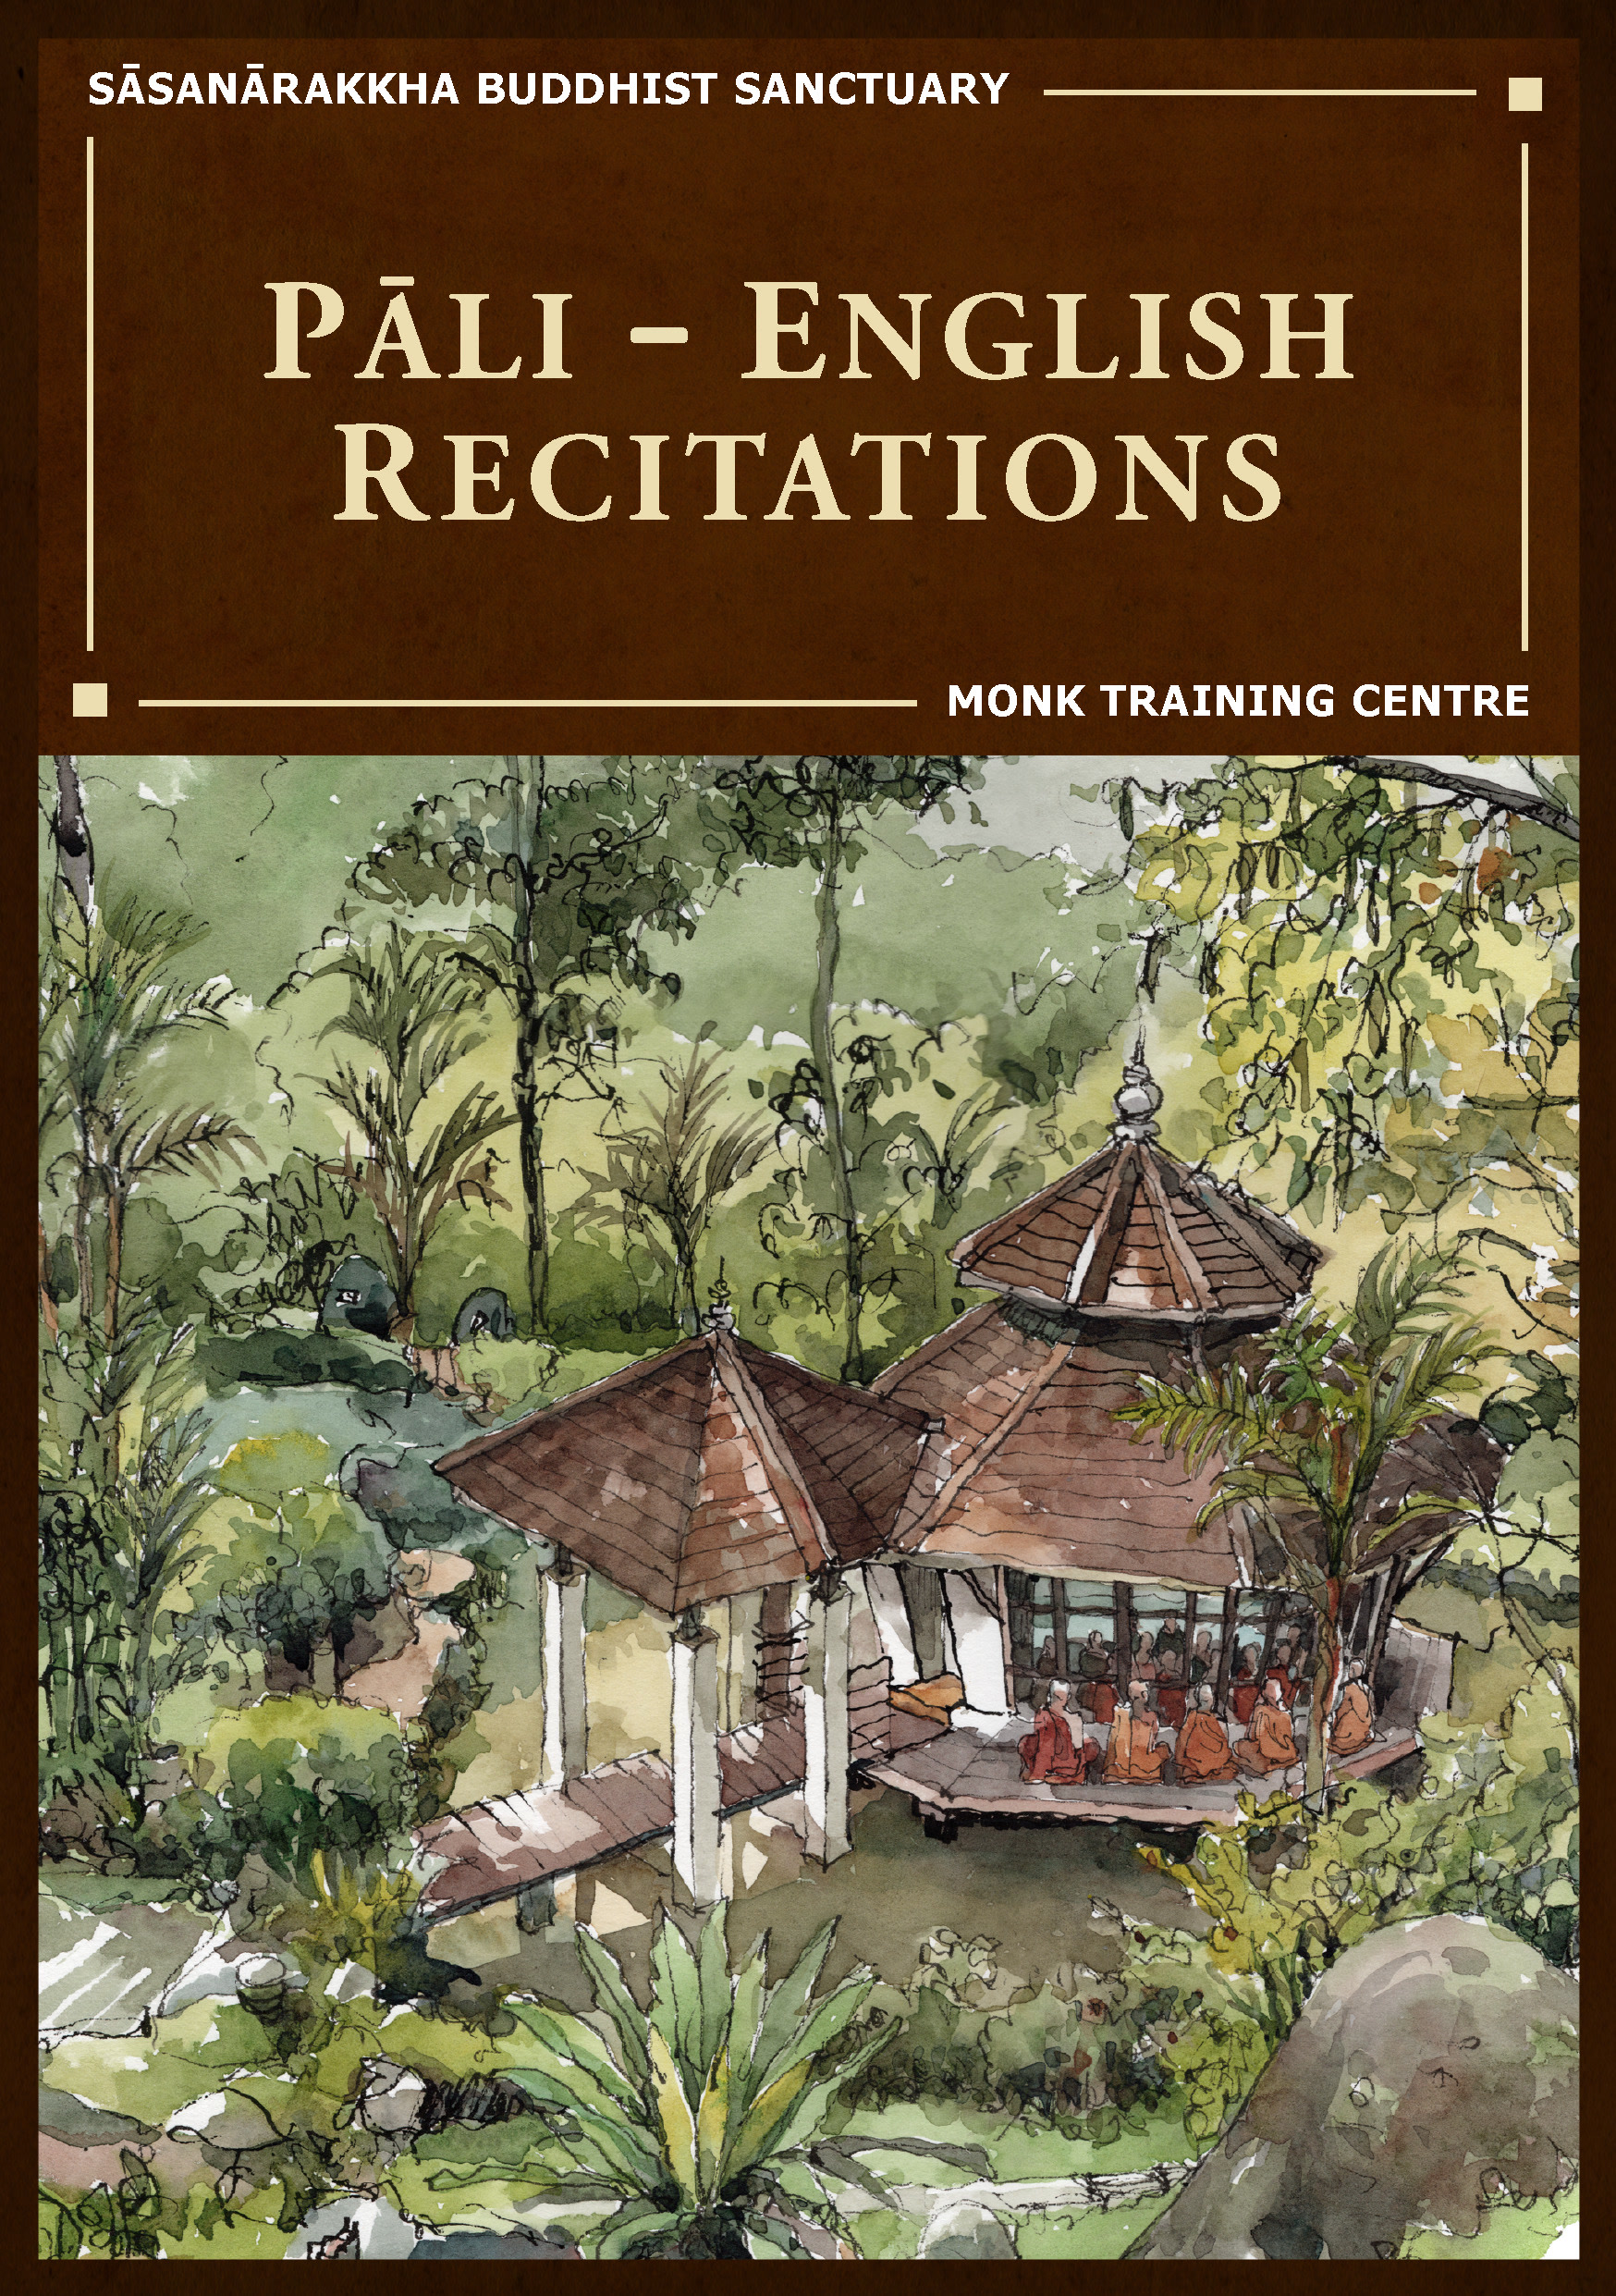
\includegraphics[height=\paperheight]{./assets/images/A5/front_cover_compressed_A5.jpg}}
\fi

\ifninebythirteenversion
  \photoFullBleed{./assets/images/9x13/front_cover_9x13.png}
  \photoFullBleed{robe_divider_left_9x13.png}
  \photoFullBleed{robe_divider_right_9x13.png}
\fi

\ifbfiveversion
  \photoFullBleed{./assets/images/B5/front_cover_B5.png}
  \photoFullBleed{robe_divider_left_B5.png}
  \photoFullBleed{robe_divider_right_B5.png}
\fi

% Title page, copyright, acknowledgments
\pagestyle{empty}

\cleartorecto
\thispagestyle{empty}

\vspace*{3em}

{\centering

  \settowidth{\titleLength}{%
    {\Large\chapterTitleFont\textsc{\MakeUppercase{{Pāli-English Recitations}}}}%
  }

  % 'SBS' on title page
  \ifafive {\Huge\fontsize{64}{16}\sbsFont SBS}\\[1.0\baselineskip] \fi
  \ifninebythirteen {\Huge\fontsize{42.5}{11}\sbsFont SBS}\\[1.0\baselineskip] \fi
  \ifbfive {\Huge\fontsize{80}{16}\sbsFont SBS}\\[1.0\baselineskip] \fi

  % 'Monk Training Centre'
  \ifafive \setlength{\xheight}{\heightof{X}}
    {\Huge\chapterTitleFont\textsc{{\thesubtitle\linebreak}}}\\[0.2\baselineskip] \fi
  \ifninebythirteen {\fontsize{16}{14}\chapterTitleFont\textsc{{\thesubtitle\linebreak}}}\\[0.2\baselineskip] \fi
  \ifbfive \setlength{\xheight}{\heightof{X}}
    {\fontsize{30}{14}\chapterTitleFont\textsc{{\thesubtitle\linebreak}}}\\[0.2\baselineskip] \fi

  % Ornament
  \ifafive \raisebox{0.5\xheight}{\pgfornament[color=sbs-brown,width=7cm,scale=1,ydelta=0pt,symmetry=c]{84}}\\[1.4\baselineskip] \fi
  \ifninebythirteen \raisebox{0.5\xheight}{\pgfornament[color=sbs-brown,width=4.5cm,scale=1,ydelta=0pt,symmetry=c]{84}}\\[1.4\baselineskip] \fi
  \ifbfive \raisebox{0.5\xheight}{\pgfornament[color=sbs-brown,width=8.5cm,scale=1,ydelta=0pt,symmetry=c]{84}}\\[1.4\baselineskip] \fi


  % 'Pali-English Recitations'
  \ifafive {\Large\scshape Pāli-English Recitations}\\[2.5\baselineskip] \fi
  \ifninebythirteen {\fontsize{10}{12}\scshape Pāli-English Recitations}\\[2.5\baselineskip] \fi
  \ifbfive {\fontsize{18.5}{12}\scshape Pāli-English Recitations}\\[2.5\baselineskip] \fi

  % Dhamma quote
  {\quote ``In whatever way a bhikkhu recites the Dhamma in detail as he has heard it and learned it, in just that way, in relation to that Dhamma, he experiences inspiration in the meaning and inspiration in the Dhamma. As he does so, joy arises in him. When he is joyful, rapture arises. For one with a rapturous mind, the body becomes tranquil. One tranquil in body feels pleasure. For one feeling pleasure, the mind becomes concentrated.''\\}
  \ifafive \smallskip AN 5.26\\[1.4\baselineskip]\fi
  \ifninebythirteen \smallskip \fontsize{8}{14}\selectfont AN 5.26\\[1.4\baselineskip]\fi
  %% \ifbfive \smallskip \fontsize{8.5}{14}\selectfont AN 5.26\\[1.4\baselineskip]\fi
  \ifbfive \smallskip AN 5.26\\[1.4\baselineskip]\fi
}



\cleartoverso
\thispagestyle{empty}

{%

  \ifafive \fontsize{10}{16}\selectfont \fi
  \ifninebythirteen \fontsize{7.5}{11}\selectfont \fi
  \ifbfive \fontsize{12}{20}\selectfont \fi
  \centering
  \setlength{\parindent}{0pt}%

  \ifafive \vspace{0.5cm} \fi
  \ifninebythirteen \vspace{0.4cm} \fi
  \ifbfive \vspace{0.5cm} \fi

  \copyright\ \thePublisher, 2025\\
  c/o 160, Lorong 3, Jalan Merdeka, 34000 Taiping, Perak, Malaysia\\
  \ifdigital
    \else
  ISBN \theISBN
  \fi

  \ifafive \vspace{0.5cm} \fi
  \ifninebythirteen \vspace{0.3cm} \fi
  \ifbfive \vspace{0.5cm} \fi

  This book is for free distribution only;\\
  it may not be sold.

  \ifafive \vspace{0.5cm} \fi
  \ifninebythirteen \vspace{0.3cm} \fi
  \ifbfive \vspace{0.5cm} \fi

  Download this book as a PDF, EPUB, MOBI, AZW3\\
  at the following address:\\
  \href{https://sasanarakkha.org/recitations}{https://sasanarakkha.org/recitations}

Accompanying audio recordings can be found at:
\href{https://www.youtube.com/SasanarakkhaBuddhistSanctuary}{https://www.youtube.com/SasanarakkhaBuddhistSanctuary}

  \ifafive \vspace{0.5cm} \fi
  \ifninebythirteen \vspace{0.3cm} \fi
  \ifbfive \vspace{0.5cm} \fi

  Project Manager: Ā. Ariyadhammika\\
  Editor: Ā. Pāladhammika\\
  Typesetting: Aj. Gambhiro, Ā. Pāladhammika\\
  Translators: Ā. Aggacitta, Ā. Bodhi, Aj. Kevalī, Ā. Sujāto, M. Walshe\\
  Endnotes: Ā. Ariyadhammika\\
  Watercolor Paintings: Lim Jee Yuan

  \ifafive \vspace{0.5cm} \fi
  \ifninebythirteen \vspace{0.3cm} \fi
  \ifbfive \vspace{0.5cm} \fi

  This work is licensed under a Creative Commons\\
  Attribution-NonCommercial-NoDerivatives 4.0 International~License.

  % Produced with the \LaTeX\ typesetting system,\\
  % set in Libertinus Serif.

  \ifafive  \vspace{0.5cm} \fi
  \ifninebythirteen \vspace{0.3cm} \fi
  \ifbfive \vspace{0.5cm} \fi

  \ifdigital
    This version was created on:\\
    \today \space at \currenttime\\
  \fi

  \ifafive \vspace{0.5cm} \fi
  \ifninebythirteen \vspace{0.15cm} \fi
  \ifbfive \vspace{0.5cm} \fi

  \theEditionInfo

}

\ifdigital

\else

\clearpage

\fi



\cleartorecto
\thispagestyle{empty}

{

  \setlength{\parskip}{10pt}

  \ifafive {\centering\fontsize{16}{25}\selectfont \textsc{We Wish To Gratefully Acknowledge} \par} \fi
  \ifninebythirteen {\centering\fontsize{10}{18}\selectfont \textsc{We Wish To Gratefully Acknowledge} \par} \fi
  \ifbfive {\centering\fontsize{18.5}{25}\selectfont \textsc{We Wish To Gratefully Acknowledge} \par} \fi


  The Saṅghas of Wat Pah Nanachat (WPN), Amaravati, and Abhayagiri for allowing the use of material from their respective chanting books, the late Ven. Dr. Saddhātissa and Mr. Maurice Walshe for their English translations, as well as Ven. Bhikkhu Bodhi for granting permission to use and slightly adapt his translations. Various Saṅgha members of SBS Monk Training Centre, who contributed in the compilation of an interesting selection of chants, as well as for providing countless suggestions to help improve the English translations.

  \linkdest{endnote1-body}
  Additional information on translations, as well as deviations\makeatletter\hyperlink{endnote1-appendix}\Hy@raisedlink{{\pagenote{%
        \hypertarget{endnote1-appendix}{\hyperlink{endnote1-body}{Due to the balanced and inspiring selection of chants, as well as for the sake of compatibility, WPN’s \textit{Buddhist Chanting} (2014) has served as the basis for this book. Over time, suggestions for the inclusion of additional chants, as well as occasional improvements of existing translations were incorporated. Such changes were meticulously marked down in the endnotes of the digital versions of this chanting book, so that someone familiar with the present book can straight away find the relevant differences, which can be useful when visiting a branch monastery of the Ajahn Chah lineage, in order to know in which places to revert to the original version.}}}}}\makeatother\thickspace
  from WPN's \textit{Buddhist Chanting} (2014), have been annotated by Ven. Ariyadhammika in the endnotes.


  \ifninebythirteen \smallskip \else \medskip \fi

  {\centering

    To Āyasmā Aggacitta, the founding father of\\
    Sāsanārakkha Buddhist Sanctuary.

    % \ifninebythirteen \smallskip \else \medskip \fi

    \begin{center}
      \ifafive 
\includegraphics[height=54mm]{sbs_logo_tuck_loon_brown.jpg} \fi
      \ifninebythirteen \clearpage \vspace*{\fill}
 
\includegraphics[height=80mm]{sbs_logo_tuck_loon_brown.jpg} \vspace*{\fill} \fi
      \ifbfive \vspace{1cm} 
\includegraphics[height=70mm]{sbs_logo_tuck_loon_brown.jpg}\fi
    \end{center}
  }
}



% Table of contents, schedule, purpose and benefits, abbreviations
\cleartorecto
\pagestyle{toponerow-frontmatter}
\chapterstyle{adrasteia-toc}

\pdfbookmark[section]{\contentsname}{toc}
\tableofcontents*


\chapter{Recitation Schedule}
\label{schedule}

{\centering

  {\pdfbookmark[2]{Set 1}{set1}\libertinusFont\selectfont\textbf{\textsc{\ifafive\fontsize{18}{12}\fi\ifninebythirteen\fontsize{13}{8.5}\fi\ifbfive\fontsize{22}{18}\fi\selectfont\textls*{Set 1}}}}\\
  \textsc{\ifafive\fontsize{14.4}{28}\fi\ifninebythirteen\fontsize{8.7}{17}\fi\ifbfive\fontsize{16}{33.5}\fi\selectfont
    \hyperref[buddhas-first-exclamation]{The Buddha's First Exclamation} \ifdigital\else\pageref{buddhas-first-exclamation}\fi\\
    \hyperref[wheel-of-dhamma-abridged]{Turning the Wheel of Dhamma} \ifdigital\else\pageref{wheel-of-dhamma-abridged}\fi\\
    \hyperref[true-false-refuges]{Going to True and False Refuges} \ifdigital\else\pageref{true-false-refuges}\fi\\
    \hyperref[four-great-references]{The Four Great References} \ifdigital\else\pageref{four-great-references}\fi\\
    \hyperref[patimokkha-exhortation]{The Pāṭimokkha Exhortation} \ifdigital\else\pageref{patimokkha-exhortation}\fi\\
    \hyperref[buddhas-final-instruction]{The Buddha's Final Instruction} \ifdigital\else\pageref{buddhas-final-instruction}\fi\\
    \hyperref[uddissanadhitthana]{Sharing and Aspirations (Pāli)} \ifdigital\else\pageref{uddissanadhitthana}\fi\\
    \hyperref[closing-homage]{Closing Homage (Pāli-English)} \ifdigital\else\pageref{closing-homage}\fi\\
  }

  \ifafive\vspace{1.0cm}\fi
  \ifninebythirteen\vspace{0.8cm}\fi
  \ifbfive\vspace{1.0cm}\fi

  {\pdfbookmark[2]{Set 2}{set2}\libertinusFont\selectfont\textbf{\textsc{\ifafive\fontsize{18}{12}\fi\ifninebythirteen\fontsize{13}{8.5}\fi\ifbfive\fontsize{22}{18}\fi\selectfont\textls*{Set 2}}}}\\
  \textsc{\ifafive\fontsize{14.4}{28}\fi\ifninebythirteen\fontsize{8.7}{17}\fi\ifbfive\fontsize{16}{33.5}\fi\selectfont
    \hyperref[characteristic-of-not-self]{The Discourse on the Characteristic of Not-Self} \ifdigital\else\pageref{characteristic-of-not-self}\fi\\
    \hyperref[exposition-on-burning]{The Discourse on the Exposition on Burning} \ifdigital\else\pageref{exposition-on-burning}\fi\\
    \hyperref[gradual-training]{The Gradual Training} \ifdigital\else\pageref{gradual-training}\fi\\
    \hyperref[sharing-aspirations]{Sharing and Aspirations (English)} \ifdigital\else\pageref{sharing-aspirations}\fi\\
    \hyperref[closing-homage]{Closing Homage (English)} \ifdigital\else\pageref{closing-homage}\fi\\
  }

  \clearpage

  {\pdfbookmark[2]{Set 3}{set3}\libertinusFont\selectfont\textbf{\textsc{\ifafive\fontsize{18}{12}\fi\ifninebythirteen\fontsize{13}{8.5}\fi\ifbfive\fontsize{22}{18}\fi\selectfont\textls*{Set 3}}}}\\

\textsc{\ifafive\fontsize{14.4}{28}\fi\ifninebythirteen\fontsize{8.7}{17}\fi\ifbfive\fontsize{16}{33.5}\fi\selectfont
    \hyperref[noble-eightfold-path]{The Noble Eightfold Path} \ifdigital\else\pageref{noble-eightfold-path}\fi\\
    \hyperref[repulsiveness-of-food]{The Repulsiveness of Food} \ifdigital\else\pageref{repulsiveness-of-food}\fi\\
    \hyperref[requisites-for-awakening]{Requisites for Awakening} \ifdigital\else\pageref{requisites-for-awakening}\fi\\
    \hyperref[principles-of-non-decline]{Principles of Non-Decline} \ifdigital\else\pageref{principles-of-non-decline}\fi\\
    \hyperref[protection]{On Protection} \ifdigital\else\pageref{protection}\fi\\
    \hyperref[sharing-all-merits]{Sharing of All Merits} \ifdigital\else\pageref{sharing-all-merits}\fi\\
    \hyperref[closing-homage]{Closing Homage (Pāli-English)} \ifdigital\else\pageref{closing-homage}\fi\\
  }

  \ifafive\vspace{1.0cm}\fi
  \ifninebythirteen\vspace{0.8cm}\fi
  \ifbfive\vspace{1.0cm}\fi

  {\pdfbookmark[2]{Set 4}{set4}\libertinusFont\selectfont\textbf{\textsc{\ifafive\fontsize{18}{12}\fi\ifninebythirteen\fontsize{13}{8.5}\fi\ifbfive\fontsize{22}{18}\fi\selectfont\textls*{Set 4}}}}\\

\textsc{\ifafive\fontsize{14.4}{28}\fi\ifninebythirteen\fontsize{8.7}{17}\fi\ifbfive\fontsize{16}{33.5}\fi\selectfont
    \hyperref[dedication-of-offerings]{Homage to the Triple Gem} \ifdigital\else\pageref{dedication-of-offerings}\fi\\
    \hyperref[universal-well-being]{Universal Well-Being} \ifdigital\else\pageref{universal-well-being}\fi\\
    \hyperref[seven-factors-of-awakening]{The Seven Factors of Awakening} \ifdigital\else\pageref{seven-factors-of-awakening}\fi\\
    \hyperref[words-on-loving-kindness]{The Buddha's Words on Loving-Kindness} \ifdigital\else\pageref{words-on-loving-kindness}\fi\\
    \hyperref[sharing-merits-departed]{Sharing of Merits with \ifninebythirteen\\[-0.6em]\fi the Departed (Pāli-English)} \ifdigital\else\pageref{sharing-merits-departed}\fi\\
    \hyperref[sharing-merits-devas]{Sharing of Merits with the Devas (Pāli-English)} \ifdigital\else\pageref{sharing-merits-devas}\fi\\
    \hyperref[closing-homage]{Closing Homage (Pāli-English)} \ifdigital\else\pageref{closing-homage}\fi\\
  }

  \clearpage

  {\pdfbookmark[2]{Set 5}{set5}\libertinusFont\selectfont\textbf{\textsc{\ifafive\fontsize{18}{12}\fi\ifninebythirteen\fontsize{13}{8.5}\fi\ifbfive\fontsize{22}{18}\fi\selectfont\textls*{Set 5}}}}\\
  \textsc{\ifafive\fontsize{14.4}{28}\fi\ifninebythirteen\fontsize{8.7}{17}\fi\ifbfive\fontsize{16}{33.5}\fi\selectfont
    \hyperref[mindfulness-of-breathing]{Mindfulness of Breathing} \ifdigital\else\pageref{mindfulness-of-breathing}\fi\\
    \hyperref[discourse-on-blessings]{The Discourse on Blessings} \ifdigital\else\pageref{discourse-on-blessings}\fi\\
    \hyperref[three-characteristics]{The Three Characteristics} \ifdigital\else\pageref{three-characteristics}\fi\\
    \hyperref[four-requisites]{The Four Requisites} \ifdigital\else\pageref{four-requisites}\fi\\
    \hyperref[five-reflections]{Five Subjects for Frequent Reflection} \ifdigital\else\pageref{five-reflections}\fi\\
    \hyperref[32-parts]{The Thirty-Two Body Parts} \ifdigital\else\pageref{32-parts}\fi\\
    \hyperref[principles-of-cordiality]{Principles of Cordiality} \ifdigital\else\pageref{principles-of-cordiality}\fi\\
    \hyperref[highest-honour-aspirations]{The Highest Honour and Aspirations} \ifdigital\else\pageref{highest-honour-aspirations}\fi\\
    \hyperref[closing-homage]{Closing Homage (Pāli-English)} \ifdigital\else\pageref{closing-homage}\fi\\
  }

  \ifafive\vspace{1.0cm}\fi
  \ifninebythirteen\vspace{0.8cm}\fi
  \ifbfive\vspace{1.0cm}\fi

  {\pdfbookmark[2]{Set 6}{set6}\libertinusFont\selectfont\textbf{\textsc{\ifafive\fontsize{18}{12}\fi\ifninebythirteen\fontsize{13}{8.5}\fi\ifbfive\fontsize{22}{18}\fi\selectfont\textls*{Set 6}}}}\\
  \textsc{\ifafive\fontsize{14.4}{28}\fi\ifninebythirteen\fontsize{8.7}{17}\fi\ifbfive\fontsize{16}{33.5}\fi\selectfont
    \hyperref[anatta-lakkhana]{Anatta-lakkhaṇa Sutta} \ifdigital\else\pageref{anatta-lakkhana}\fi\\
    \hyperref[striving-according-to-dhamma]{Striving According to the Dhamma} \ifdigital\else\pageref{striving-according-to-dhamma}\fi\\
    \hyperref[divine-abidings]{The Divine Abidings} \ifdigital\else\pageref{divine-abidings}\fi\\
    \hyperref[ten-reflections]{Ten Subjects for Frequent Reflection\\ \ifafive\vspace{-0.4cm}\fi \ifbfive\vspace{-0.4cm}\fi \ifninebythirteen\vspace{-0.2cm}\fi by One Gone Forth} \ifdigital\else\pageref{ten-reflections}\fi\\
    \hyperref[sharing-aspirations]{Sharing and Aspirations (English)} \ifdigital\else\pageref{sharing-aspirations}\fi\\
    \hyperref[closing-homage]{Closing Homage (Pāli-English)} \ifdigital\else\pageref{closing-homage}\fi\\
  }

  \clearpage

  {\pdfbookmark[2]{Set 7}{set7}\libertinusFont\selectfont\textbf{\textsc{\ifafive\fontsize{18}{12}\fi\ifninebythirteen\fontsize{13}{8.5}\fi\ifbfive\fontsize{22}{18}\fi\selectfont\textls*{Set 7}}}}\\
  \textsc{\ifafive\fontsize{14.4}{28}\fi\ifninebythirteen\fontsize{8.7}{17}\fi\ifbfive\fontsize{16}{33.5}\fi\selectfont
    \hyperref[dependent-origination]{Dependent Origination} \ifdigital\else\pageref{dependent-origination}\fi\\
    \hyperref[dhamma-in-brief]{The Dhamma in Brief} \ifdigital\else\pageref{dhamma-in-brief}\fi\\
    \hyperref[uddissanadhitthana]{Sharing and Aspirations (Pāli)} \ifdigital\else\pageref{uddissanadhitthana}\fi\\
    \hyperref[closing-homage]{Closing Homage (Pāli-English)} \ifdigital\else\pageref{closing-homage}\fi\\
  }

  \ifafive\vspace{1.0cm}\fi
  \ifninebythirteen\vspace{0.8cm}\fi
  \ifbfive\vspace{1.0cm}\fi

  {\pdfbookmark[2]{Set 8}{set8}\libertinusFont\selectfont\textbf{\textsc{\ifafive\fontsize{18}{12}\fi\ifninebythirteen\fontsize{13}{8.5}\fi\ifbfive\fontsize{22}{18}\fi\selectfont\textls*{Set 8}}}}\\
  \textsc{\ifafive\fontsize{14.4}{28}\fi\ifninebythirteen\fontsize{8.7}{17}\fi\ifbfive\fontsize{16}{33.5}\fi\selectfont
    \hyperref[aditta-pariyaya]{Āditta-Pariyāya Sutta} \ifdigital\else\pageref{aditta-pariyaya}\fi\\
    \hyperref[burdens]{The Burdens} \ifdigital\else\pageref{burdens}\fi\\
    \hyperref[respect-for-the-dhamma]{Respect for the Dhamma} \ifdigital\else\pageref{respect-for-the-dhamma}\fi\\
    \hyperref[single-excellent-night]{A Single Excellent Night} \ifdigital\else\pageref{single-excellent-night}\fi\\
    \hyperref[ratthapala]{From the Elder Raṭṭhapāla}  \ifdigital\else\pageref{ratthapala}\fi\\
    \hyperref[parapariya]{From the Elder Pārāpariya} \ifdigital\else\pageref{parapariya}\fi\\
    \hyperref[misc-verses]{Miscellaneous Verses} \ifdigital\else\pageref{misc-verses}\fi\\
    \hyperref[highest-honour-aspirations]{The Highest Honour and Aspirations} \ifdigital\else\pageref{highest-honour-aspirations}\fi\\
    \hyperref[closing-homage]{Closing Homage (Pāli-English)} \ifdigital\else\pageref{closing-homage}\fi\\
  }

  \clearpage

  {\pdfbookmark[2]{Set 9}{set9}\libertinusFont\selectfont\textbf{\textsc{\ifafive\fontsize{18}{12}\fi\ifninebythirteen\fontsize{13}{8.5}\fi\ifbfive\fontsize{22}{18}\fi\selectfont\textls*{Set 9}}}}\\
  \textsc{\ifafive\fontsize{14.4}{28}\fi\ifninebythirteen\fontsize{8.7}{17}\fi\ifbfive\fontsize{16}{33.5}\fi\selectfont
    \hyperref[invitation-to-the-devas]{Protective Recitations (Pāli)} \ifdigital\else\pageref{invitation-to-the-devas}\fi\\
    \hyperref[sharing-merits-departed]{Sharing of Merits with the Departed (Pāli)} \ifdigital\else\pageref{sharing-merits-departed}\fi\\
    \hyperref[sharing-merits-devas]{Sharing of Merits with the Devas (Pāli)} \ifdigital\else\pageref{sharing-merits-devas}\fi\\
    \hyperref[closing-homage]{Closing Homage (Pāli)} \ifdigital\else\pageref{closing-homage}\fi\\
  }

  \ifafive\vspace{1.0cm}\fi
  \ifninebythirteen\vspace{0.8cm}\fi
  \ifbfive\vspace{1.0cm}\fi

  {\pdfbookmark[2]{Set 10}{set10}\libertinusFont\selectfont\textbf{\textsc{\ifafive\fontsize{18}{12}\fi\ifninebythirteen\fontsize{13}{8.5}\fi\ifbfive\fontsize{22}{18}\fi\selectfont\textls*{Set 10}}}}\\
\textsc{\ifafive\fontsize{14.4}{28}\fi\ifninebythirteen\fontsize{8.7}{17}\fi\ifbfive\fontsize{16}{33.5}\fi\selectfont
    \hyperref[passage-on-preliminary-paying-of-homage-funeral]{Funeral Recitations (Pāli)} \ifdigital\else\pageref{passage-on-preliminary-paying-of-homage-funeral}\fi\\
    \hyperref[recollection-of-impermanence]{Recollection of Impermanence} \ifdigital\else\pageref{recollection-of-impermanence}\fi\\
    \hyperref[just-as-rivers]{Thanksgiving Recitations} \ifdigital\else\pageref{just-as-rivers}\fi\\
    \hyperref[sharing-all-merits]{Sharing of All Merits} \ifdigital\else\pageref{sharing-all-merits}\fi\\
    \hyperref[closing-homage]{Closing Homage (Pāli-English)} \ifdigital\else\pageref{closing-homage}\fi\\
  }}


\input{./tex/purpose-and-benefits.tex}

\chapter{Abbreviations}
\label{abbreviations}

\ifafive
\begin{tabular}{@{}ll@{}}
  \anglebracketleft\ \hspace{-0.5mm}... \hspace{-0.85mm}\anglebracketright\ & \hspace{1.30mm}Only recited by the leader \\
  \hspace{0.1cm} \abbrbreathmark\ & \hspace{1.45mm}Breathing pause \\
\end{tabular}
\fi

\ifninebythirteen
\begin{tabular}{@{}ll@{}}
  \anglebracketleft\ \hspace{-0.5mm}... \hspace{-0.70mm}\anglebracketright\ & \hspace{1.10mm}Only recited by the leader \\
  \hspace{0.1cm} \abbrbreathmark\ & \hspace{1.20mm}Breathing pause \\
\end{tabular}
\fi

\ifbfive
\begin{tabular}{@{}ll@{}}
  \anglebracketleft\ \hspace{-0.5mm}... \hspace{-0.85mm}\anglebracketright\ & \hspace{2.70mm}Only recited by the leader \\
  \hspace{0.2cm} \abbrbreathmark\ & \hspace{2.90mm}Breathing pause \\
\end{tabular}
\fi

\ifninebythirteen

\vspace{-0.6em}
\begin{tabular}{@{}llll@{}}
  DN    & Dīgha Nikāya                                        \\
  MN    & Majjhima Nikāya                                     \\
  SN    & Saṁyutta Nikāya                                     \\
  AN    & Aṅguttara Nikāya                                    \\
  Kp    & Khuddakapāṭha                                       \\
  Dhp   & Dhammapada                                          \\
  Ud    & Udāna                                               \\
  Snp   & Sutta Nipāta                                        \\
  Thag  & Theragāthā                                          \\
  Ja    & Jātaka                                              \\
  Pv    & Petavatthu                                          \\
  Vibh  & Abhidhamma Vibhaṅga                                 \\
  Dhs   & Dhammasaṅganī                                       \\
  A     & Aṭṭhakathā (Commentary)                             \\
  MJG   & Mahā-jaya-maṅgala-gāthā (Sri Lanka)                 \\
  Trad  & Traditional post-canonical verses                   \\
  WPN   & Wat Pah Nanachat                                    \\
\end{tabular}

\else

\begin{tabular}{@{}llll@{}}
  DN    & Dīgha Nikāya                                        \\
  MN    & Majjhima Nikāya                                     \\
  SN    & Saṁyutta Nikāya                                     \\
  AN    & Aṅguttara Nikāya                                    \\
  Kp    & Khuddakapāṭha                                       \\
  Dhp   & Dhammapada                                          \\
  Ud    & Udāna                                               \\
  Snp   & Sutta Nipāta                                        \\
  Thag  & Theragāthā                                          \\
  Ja    & Jātaka                                              \\
  Pv    & Petavatthu                                          \\
  Vibh  & Abhidhamma Vibhaṅga                                 \\
  Dhs   & Dhammasaṅganī                                       \\
\end{tabular}

\begin{tabular}{@{}llll@{}}
  A     & Aṭṭhakathā (Commentary)                             \\
  MJG   & Mahā-jaya-maṅgala-gāthā (Sri Lanka)                 \\
  Trad  & Traditional post-canonical verses                   \\
  WPN   & Wat Pah Nanachat
\end{tabular}

\medskip

\fi



\chapterstyle{adrasteia-frontmatter}

% Main matter
\mainmatter
\pagestyle{toponerow}

\cleartorecto

% Chapters
{\raggedright
	\input{./tex/recitations/homage.tex}
	\input{./tex/recitations/verses.tex}
	\input{./tex/recitations/teachings.tex}
	\input{./tex/recitations/reflections.tex}
	
\ifdigitalversion
  \chapterOpeningPage{cardinal_discourses_compressed_A5.jpg}
\else
  \chapterOpeningPage{cardinal_discourses_A5.jpg}
\fi

\ifninebythirteenversion
  \chapterOpeningPage{cardinal_discourses_9x13.png}
\fi

\ifbfiveversion
  \chapterOpeningPage{cardinal_discourses_B5.png}
\fi

\chapter{Cardinal Discourses}

\ifbfiveversion
  \photoFullBleed{assets/images/B5/brown_divider_B5.pdf}
\fi

\ifninebythirteenversion
  \photoFullBleed{assets/images/9x13/brown_divider_9x13.pdf}\fi

\input{./tex/recitations/cardinal-discourses/dhammacakkappavattana.tex}

\clearpage

\input{./tex/recitations/cardinal-discourses/dhammacakkappavattana-eng.tex}

\clearpage

\input{./tex/recitations/cardinal-discourses/anattalakkhana.tex}

\clearpage

\input{./tex/recitations/cardinal-discourses/anattalakkhana-eng.tex}

\clearpage

\input{./tex/recitations/cardinal-discourses/adittapariyaya.tex}

\clearpage

\input{./tex/recitations/cardinal-discourses/adittapariyaya-eng.tex}

\clearpage


	\input{./tex/recitations/thanksgiving-recitations.tex}
	\input{./tex/recitations/protective-recitations.tex}
	\input{./tex/recitations/funeral-recitations.tex}
	\input{./tex/recitations/sharing-of-merits.tex}
}

% Appendix
\appendix

\ifdigitalversion
  \chapterOpeningPage{appendix_compressed_A5.jpg}
\else
  \chapterOpeningPage{appendix_A5.jpg}
\fi

\ifninebythirteenversion
  \chapterOpeningPage{appendix_9x13.jpg}
\fi

\ifbfiveversion
  \chapterOpeningPage{appendix_B5.jpg}
\fi

\ifafiveversion\addtocontents{toc}{\protect\clearpage}\fi
\chapter{Appendix}

\ifbfiveversion
  \includepdf[pages=-]{assets/graphics/brown-texture_B5.pdf}
\fi

\ifninebythirteenversion
  \includepdf[pages=-]{assets/graphics/brown-texture_9x13.pdf}
\fi

\clearpage


\input{./tex/refuge-trainings.tex}
\input{./tex/phonetics-pronunciation.tex}
\input{./tex/guidelines.tex}

% Back matter
\backmatter
\printpagenotes % Print endnotes
\input{./tex/copyright-details.tex}

\ifbfiveversion
  \includepdf[pages=-,pagecommand={\thispagestyle{empty}}]{assets/images/graphics/donor-list.pdf}
  \photoFullBleed{robe_divider_left_B5.png}
  \photoFullBleed{robe_divider_right_B5.png}
\fi

\ifninebythirteenversion
  \photoFullBleed{robe_divider_left_9x13.png}
  \photoFullBleed{robe_divider_right_9x13.png}
\fi

\emptyUntilEven % Add blank page if necessary

\ifdigitalversion
  \clearpage
  \digitalCover{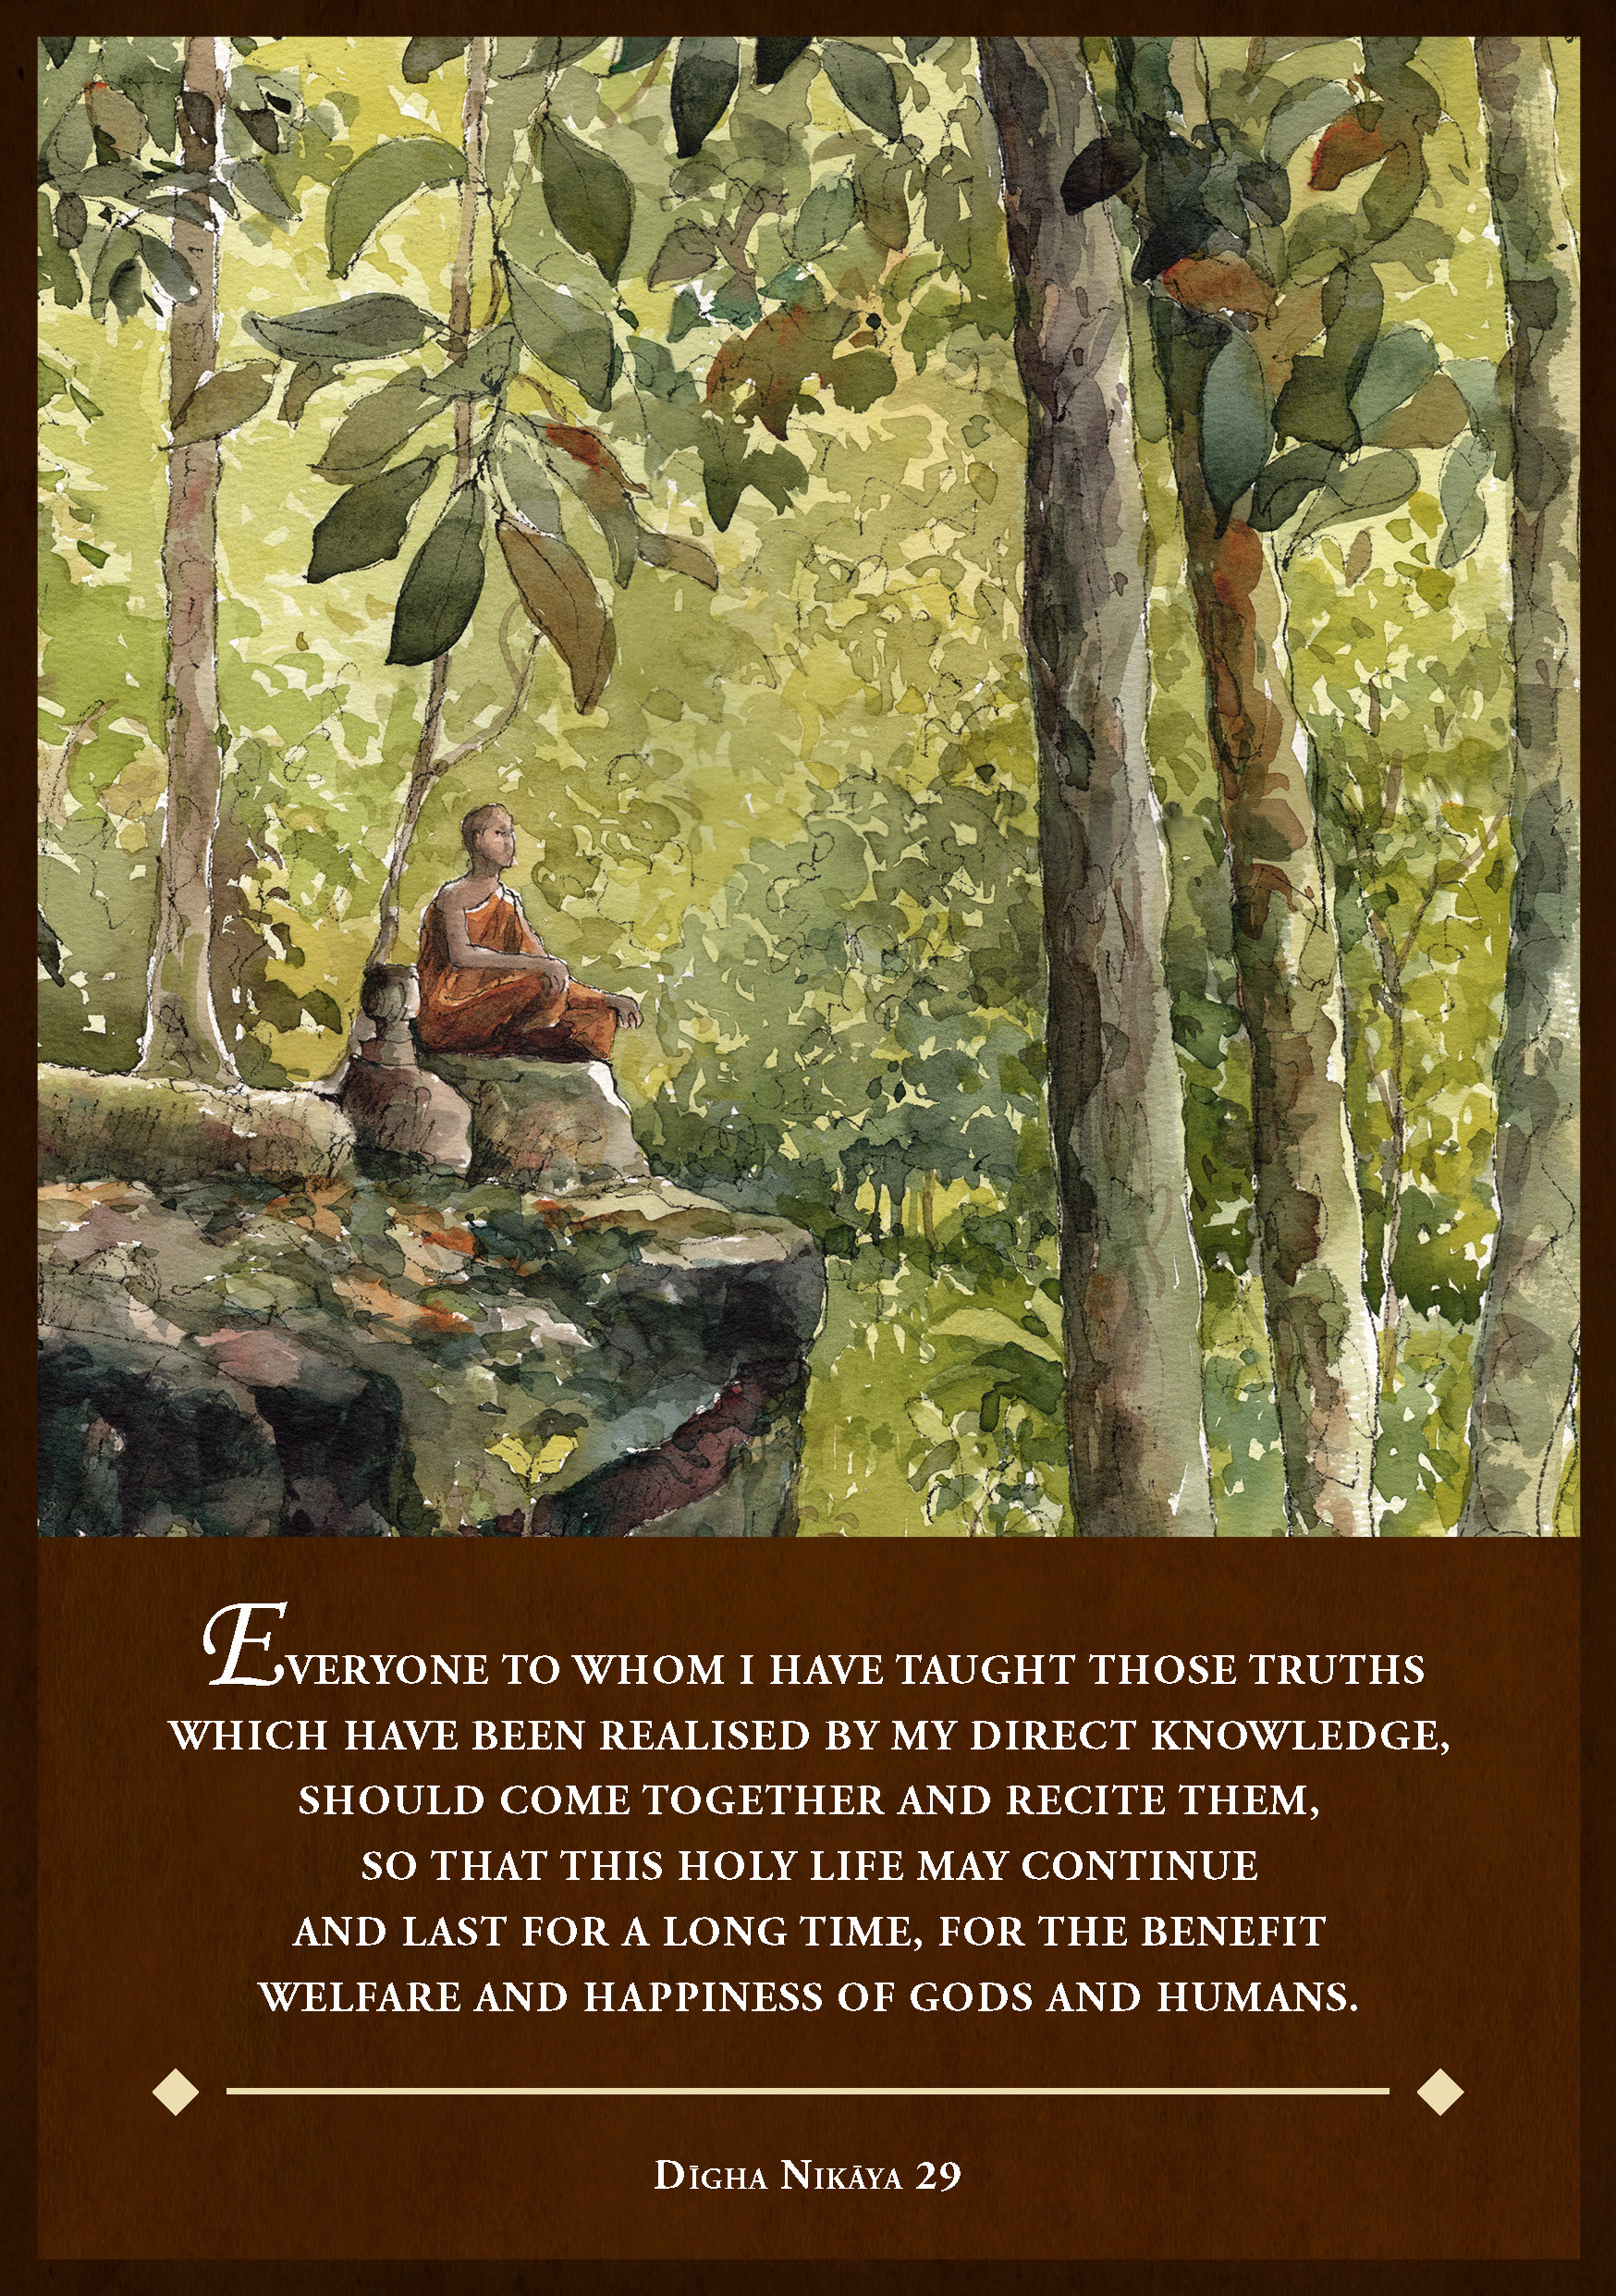
\includegraphics[height=\paperheight]{./assets/images/A5/back_cover_compressed_A5.jpg}}
\fi

\ifninebythirteenversion
  \photoFullBleed{./assets/images/9x13/back_cover_9x13.png}
\fi

\ifbfiveversion
  \photoFullBleed{./assets/images/B5/back_cover_B5.png}
\fi

\end{document}
